\documentclass[german,10pt]{book}


\usepackage{makeidx}
\usepackage{babel}            % Sprachunterstuetzung
\usepackage{amsmath}          % AMS "Grundpaket"
\usepackage{amssymb,amsfonts,amsthm,amscd} 
\usepackage{mathrsfs}
\usepackage{rotating}
\usepackage{sidecap}
\usepackage{graphicx}
\usepackage{color}
\usepackage{fancybox}
\usepackage{tikz}
\usetikzlibrary{arrows,snakes,backgrounds}
\usepackage{hyperref}
\hypersetup{colorlinks=true,
                    linkcolor=blue,
                    filecolor=magenta,
                    urlcolor=cyan,
                    pdftitle={Overleaf Example},
                    pdfpagemode=FullScreen,}
%\newcommand{\hyperref}[1]{\ref{#1}}
%
\definecolor{Gray}{gray}{0.80}
\DeclareMathSymbol{,}{\mathord}{letters}{"3B}
%
\newcounter{num}
\renewcommand{\thenum}{\arabic{num}}
\newenvironment{anmerkungen}
   {\begin{list}{(\thenum)}{%
   \usecounter{num}%
   \leftmargin0pt
   \itemindent5pt
   \topsep0pt
   \labelwidth0pt}%
   }{\end{list}}
%
\renewcommand{\arraystretch}{1.15}                % in Formeln und Tabellen   
\renewcommand{\baselinestretch}{1.15}                 % 1.15 facher
                                                      % Zeilenabst.
\newcommand{\Anmerkung}[1]{{\begin{footnotesize}#1 \end{footnotesize}}\\[0.2cm]}
\newcommand{\comment}[1]{}
\setlength{\parindent}{0em}           % Nicht einruecken am Anfang der Zeile 

\setlength{\textwidth}{15.4cm}
\setlength{\textheight}{23.0cm}
\setlength{\oddsidemargin}{1.0mm} 
\setlength{\evensidemargin}{-6.5mm}
\setlength{\topmargin}{-10mm} 
\setlength{\headheight}{0mm}
\newcommand{\identity}{{\bf 1}}
%
\newcommand{\vs}{\vspace{0.3cm}}
\newcommand{\noi}{\noindent}
\newcommand{\leer}{}

\newcommand{\engl}[1]{[\textit{#1}]}
\parindent 1.2cm
\sloppy



\makeindex

\begin{document}

\mbox{~}
\vspace{3cm}

\begin{center}
{\bf\LARGE Ausgew\"ahlte Kapitel der Modernen Physik}\\[0.5cm] 
{\large Thomas Filk}\\[1.5cm]
Skript zur Vorlesung\\[2cm]
(Version vom 17.\,Mai\,2023)
\end{center}
\thispagestyle{empty}


\newpage

%\documentclass[german,12pt]{book}   
\usepackage{makeidx}
\usepackage{babel}            % Sprachunterstuetzung
\usepackage{amsmath}          % AMS "Grundpaket"
\usepackage{amssymb,amsfonts,amsthm,amscd} 
\usepackage{mathrsfs}
\usepackage{rotating}
\usepackage{sidecap}
\usepackage{graphicx}
\usepackage{color}
\usepackage{fancybox}
\usepackage{tikz}
\usetikzlibrary{arrows,snakes,backgrounds}
\usepackage{hyperref}
\hypersetup{colorlinks=true,
                    linkcolor=blue,
                    filecolor=magenta,
                    urlcolor=cyan,
                    pdftitle={Overleaf Example},
                    pdfpagemode=FullScreen,}
%\newcommand{\hyperref}[1]{\ref{#1}}
%
\definecolor{Gray}{gray}{0.80}
\DeclareMathSymbol{,}{\mathord}{letters}{"3B}
%
\newcounter{num}
\renewcommand{\thenum}{\arabic{num}}
\newenvironment{anmerkungen}
   {\begin{list}{(\thenum)}{%
   \usecounter{num}%
   \leftmargin0pt
   \itemindent5pt
   \topsep0pt
   \labelwidth0pt}%
   }{\end{list}}
%
\renewcommand{\arraystretch}{1.15}                % in Formeln und Tabellen   
\renewcommand{\baselinestretch}{1.15}                 % 1.15 facher
                                                      % Zeilenabst.
\newcommand{\Anmerkung}[1]{{\begin{footnotesize}#1 \end{footnotesize}}\\[0.2cm]}
\newcommand{\comment}[1]{}
\setlength{\parindent}{0em}           % Nicht einruecken am Anfang der Zeile 

\setlength{\textwidth}{15.4cm}
\setlength{\textheight}{23.0cm}
\setlength{\oddsidemargin}{1.0mm} 
\setlength{\evensidemargin}{-6.5mm}
\setlength{\topmargin}{-10mm} 
\setlength{\headheight}{0mm}
\newcommand{\identity}{{\bf 1}}
%
\newcommand{\vs}{\vspace{0.3cm}}
\newcommand{\noi}{\noindent}
\newcommand{\leer}{}

\newcommand{\engl}[1]{[\textit{#1}]}
\parindent 1.2cm
\sloppy

     \begin{document}

\chapter*{Vorwort}
\addcontentsline{toc}{chapter}{Vorwort}
\thispagestyle{empty}

Der vorliegende Text entstand im Zusammenhang 
mit dem Projekt, f\"ur das mir im Juni 2022 von der Wilhelm und Else Her\"aus-Stiftung
eine Seniorprofessur an der Universit\"at Freiburg verliehen wurde. Dieses Projekt
besteht in der Ausarbeitung einer Vorlesung mit dem (vorl\"aufigen) Titel
\glqq Ausgew\"ahlte Kapitel der Modernen Physik\grqq. Die Vorlesung richtet sich
speziell an Studierende  f\"ur das Lehramt Physik und soll einige Themen abdecken,
die im regul\"aren Studium oft nur am Rande angesprochen werden, die aber f\"ur
die Unterrichtspraxis relevant sein k\"onnen, auch wenn sie teilweise deutlich \"uber
die Vorgaben der Lehrpl\"ane hinausgehen.  

Die einzelnen Kapitel in diesem Text sind weitgehend unabh\"angig voneinander und
k\"onnen jeweils f\"ur sich gelesen werden. Sie bestehen aus Kurztexten zu bestimmten
Themen. Daher kommt es gelegentlich vor, dass mehrere Kapitel in einem ihrer Unterabschnitte
denselben physikalischen Sachverhalt in unterschiedlicher Ausf\"uhrlichkeit beschreiben.
Wenn dieser Sachverhalt f\"ur ein bestimmtes Thema relevant ist, wird er in diesem
Zusammenhang auch kurz beschrieben, wobei dann aber f\"ur eine ausf\"uhrlichere
Behandlung auf einen anderen Kurztext verwiesen werden kann. Aus diesem Grund hat
auch jedes Kapitel seine eigenen Literaturangaben. 

Gelegentlich wird man sich wundern, dass in einer Vorlesung zur \glqq modernen Physik\grqq\
auch die Bestimmung des Erdumfangs nach Eratosthenes oder die Physik der
Gezeiten thematisiert wird. Aber die Bestimmung des Erdumfangs ist der erste Schritt in
der kosmischen Entfernungsleiter, und dies ist ein aktuelles Forschungsgebiet, das
beispielsweise mit der Suche nach Dunkler Energie verkn\"upft ist. Die Physik der
Gezeiten h\"angt eng mit den l\"anger werdenden Tagen und dem zunehmenden Abstand
zwischen Erde und Mond zusammen, die erst im letzten Jahrhundert entdeckt wurden. 
Insofern bezieht sich \glqq moderne Physik\grqq\ nicht nur auf die Quantentheorie und die
Relativit\"atstheorie. 

Die Sammlung wird st\"andig erweitert. Mittlerweile haben auch andere Dozentinnen und
Dozenten angeboten, in dem vorgegebenen Sinne solche Kurztexte zu erstellen. Auch die bereits
vorhandenen Texte werden weiter \"uberarbeitet und an die parallel stattfindende
Vorlesung angepasst. 

%{\small
\vspace{0.3cm}

\noindent
Freiburg, Fr\"uhjahr 2023\\
Thomas~Filk
%}
%\end{document}


\addcontentsline{toc}{chapter}{Inhaltsverzeichnis}
\tableofcontents

\documentclass[german,10pt]{book}      
\usepackage{makeidx}
\usepackage{babel}            % Sprachunterstuetzung
\usepackage{amsmath}          % AMS "Grundpaket"
\usepackage{amssymb,amsfonts,amsthm,amscd} 
\usepackage{mathrsfs}
\usepackage{rotating}
\usepackage{sidecap}
\usepackage{graphicx}
\usepackage{color}
\usepackage{fancybox}
\usepackage{tikz}
\usetikzlibrary{arrows,snakes,backgrounds}
\usepackage{hyperref}
\hypersetup{colorlinks=true,
                    linkcolor=blue,
                    filecolor=magenta,
                    urlcolor=cyan,
                    pdftitle={Overleaf Example},
                    pdfpagemode=FullScreen,}
%\newcommand{\hyperref}[1]{\ref{#1}}
%
\definecolor{Gray}{gray}{0.80}
\DeclareMathSymbol{,}{\mathord}{letters}{"3B}
%
\newcounter{num}
\renewcommand{\thenum}{\arabic{num}}
\newenvironment{anmerkungen}
   {\begin{list}{(\thenum)}{%
   \usecounter{num}%
   \leftmargin0pt
   \itemindent5pt
   \topsep0pt
   \labelwidth0pt}%
   }{\end{list}}
%
\renewcommand{\arraystretch}{1.15}                % in Formeln und Tabellen   
\renewcommand{\baselinestretch}{1.15}                 % 1.15 facher
                                                      % Zeilenabst.
\newcommand{\Anmerkung}[1]{{\begin{footnotesize}#1 \end{footnotesize}}\\[0.2cm]}
\newcommand{\comment}[1]{}
\setlength{\parindent}{0em}           % Nicht einruecken am Anfang der Zeile 

\setlength{\textwidth}{15.4cm}
\setlength{\textheight}{23.0cm}
\setlength{\oddsidemargin}{1.0mm} 
\setlength{\evensidemargin}{-6.5mm}
\setlength{\topmargin}{-10mm} 
\setlength{\headheight}{0mm}
\newcommand{\identity}{{\bf 1}}
%
\newcommand{\vs}{\vspace{0.3cm}}
\newcommand{\noi}{\noindent}
\newcommand{\leer}{}

\newcommand{\engl}[1]{[\textit{#1}]}
\parindent 1.2cm
\sloppy

         \begin{document}  \setcounter{chapter}{1}


\chapter{SI-Einheiten}
% Kap 1
\label{chap_SI}

Auf ihrer 26.\ Versammlung im November 2018 hat die CGPM (Conf\'{e}rence g\'{e}n\'{e}rale des poids et mesure -
General Conference on Weights and Measures) \index{CGPM - General Conference on Weights and Measures} 
ein neues Einheitensystem (SI - Syst\'{e}me international d'unit\'{e}s)\index{SI - Internationales Einheitensystem} 
beschlossen, das am 20.\ Mai 2019 in Kraft trat. Dieses System basiert im Wesentlichen auf der
Festlegung einer Zeiteinheit sowie der Festlegung bestimmter Naturkonstanten, mit denen ausgehend von der
Zeiteinheit andere Grundeinheiten - L\"ange, Masse, Temperatur, Stromst\"arke, 
Mengeneinheit - definiert werden k\"onnen. 


\section{Das neue System der Grundeinheiten}

Das neue System der Grundeinheiten beruht auf den Festlegungen der in Tabelle \ref{tab_SI}
angegebenen Naturkonstanten.\index{Frequenz des Hyperfeinstruktur\"ubergangs in C\"asium-133}%
\index{Lichtgeschwindigkeit}\index{Planck'sche Konstante}\index{Elementarladung}%
\index{Boltzmann-Konstante}\index{Avogadro-Konstante}%

\begin{table}[htb]
\begin{tabular}{l|l|l}
Bezeichnung & Symbol & Wert und Einheit \\ \hline
Frequenz des Hyperfinestruktur\"ubergangs in C\"asium-133 & $\Delta \nu_{\rm Cs}$ &
        9\,192\,631\,770\,{\rm Hz} \\
Lichtgeschwindigkeit im Vakuum & $c$ & 299\,792\,458\,{\rm m/s} \\ 
Planck'sche Konstante & $h$ & $6,626\,070\,15 \cdot 10^{-34}\,{\rm J\,s}$ \\
Elementarladung & $e$ & $1,602\,176\,634 \cdot 10^{-19}\,{\rm C}$ \\
Boltzmann-Konstante & $k_{\rm B}$ & $1,380\,649 \cdot 10^{-23}\,{\rm J/K}$ \\
Avogadro-Konstante & $N_{\rm A}$ & $ 6,022\,140\,76 \cdot 10^{23}\,{\rm mol}^{-1}$ \\
Photometrisches Strahlungs\"aquivalent & $K_{\rm cd}$ & $683\,{\rm lm/W}$ \\[-0.1cm]
(Monochromatische Strahlung von 540\,THz) & &  \\ \hline        
\end{tabular}
\caption{\label{tab_SI}%
Die fundamentalen Konstanten zur Festlegung der SI-Basis.}
\end{table}

Das photometrische Strahlungs\"aquivalent ist eine technische Konstante, die eine physikalische
Gr\"o\ss e (eine Strahlungsleistung, ausgedr\"uckt in Watt) mit einer physiologischen Gr\"o\ss e,
einer wahrgenommenen Helligkeit - ausgedr\"uckt durch die Einheit Lumen - in Verbindung bringt. 
Hierauf werden wir nicht weiter eingehen. 

Die Definition einer fundamentalen Frequenz $\Delta \nu_{\rm Cs}$ \"uber einen bestimmten
\"Ubergang (dem Hyperfeinstruktur\"ubergang im Grundzustand)
 in einem bestimmten Atom (C\"asium-133) gibt gleichzeitig eine physikalische Realisierung
dieser Frequenz an. Atomuhren, bei denen die Frequenz des C\"asium\"ubergangs gemessen wird, 
bezeichnet man als \glqq prim\"are Zeitnormale\grqq.\index{Zeitnormale!prim\"are} 
Es gibt andere Realisierungen (\"Uberg\"ange im Wasserstoff oder in Rubidium etc.),
die aber vorher am C\"asium\"ubergang geeicht werden m\"ussen und mit mindestens derselben
Genauigkeit und Stabilit\"at reproduzierbar sein sollten. Solche Realisierungen bezeichnet man
auch als \glqq sekund\"are Zeitnormale\grqq.\index{Zeitnormale!sekund\"are} 

Die fundamentalen Einheiten - Sekunde, Meter, Kilogramm, Ampere, Kelvin, Mol (und das Candela) -
erh\"alt man nun als Kombination dieser Gr\"o\ss en. Wie diese fundamentalen Einheiten zu bestimmen
sind, ist mit Ausnahme der Sekunde nicht festgelegt. Bei der Boltzmann-Konstanten und der Avogadro-Konstanten
handelt es sich um Proportionalit\"atsfaktoren zwischen historisch festgelegten Gr\"o\ss en, die
man heute nicht mehr unterscheiden m\"usste. Die Planck'sche Konstante und die Lichtgeschwindigkeit
im Vakuum sind universelle Naturkonstanten, die in vielen Naturgesetzen auftreten und somit
auf unterschiedliche Weisen bestimmt werden k\"onnen. Das neue SI-System l\"asst diese
Bestimmung offen.  

\subsection{Die Sekunde}
\label{sec_Sekunde}

Eine Frequenz gibt an,\index{Sekunde}\index{Frequenz} 
wie oft sich ein periodisch wiederkehrendes Ereignis in einer gewissen
Zeiteinheit wiederholt. Die Einheit Hertz (Hz) legt diese Zeiteinheit auf eine Sekunde fest. 
Eine Sekunde ist somit die Zeitdauer, in der sich die Schwingungen, die dem \"Ubergang im
C\"asium entsprechen, 9\,192\,631\,770 mal wiederholen. Oder anders ausgedr\"uckt: Die 
Periodendauer einer Schwingung entspricht\index{Periodendauer} 
\begin{equation}
               T = \frac{1}{\Delta \nu_{\rm Cs}} = \frac{1}{ 9\,192\,631\,770} {\rm s} \, .
\end{equation}  
Damit ist
\begin{equation}
               1\,{\rm s}  =  9\,192\,631\,770 \, T = 9\,192\,631\,770 \, \frac{1}{\Delta \nu_{\rm Cs}} \, .
\end{equation}  
Diese Gleichung kann man auch so interpretieren, dass die Definition
\begin{equation}
               \Delta \nu_{\rm Cs}  =  9\,192\,631\,770 \, {\rm s}^{-1}
\end{equation}  
nach der Einheit Sekunde aufgel\"ost wird. 

\subsection{Das Meter}

Bereits 1975 wurde der Wert der Lichtgeschwindigkeit 
im Vakuum als Naturkonstante,\index{Meter}
wie in Tabelle \ref{tab_SI} angegeben, festgelegt. Damit l\"asst sich die Einheit f\"ur
eine L\"ange - das Meter - auf die Einheit der Zeit zur\"uckf\"uhren:
\begin{equation}
              1\,{\rm m} =                 \frac{c}{299\,792\,458} \cdot 1 \,{\rm s} = 
              \frac{9\,192\,631\,770}{299\,792\,458} \frac{c}{\Delta \nu_{\rm Cs}} 
                 \approx  30,6633189885 \frac{c}{\Delta \nu_{\rm Cs}} \, .
\end{equation}  
Diese Festlegung hat zwei \"aquivalente Interpretationen: Zum einen ist ein Meter der
1/299\,792\,458 Teil der Strecke, die das Licht im Vakuum in einer Sekunde zur\"ucklegt,
bzw.\ das 30,6633... fache der Strecke, die das Licht im Vakuum in der Zeitdauer einer Periode
der Cs-Schwingung zur\"ucklegt. Andererseits entspricht das Verh\"altnis $c/\Delta \nu$
der Wellenl\"ange einer Strahlung, die sich mit der Geschwindigkeit $c$ ausbreitet und eine
Frequenz $\Delta \nu$ hat. Also ist 1 Meter das 30,6633...-fache der 
Wellenl\"ange der Strahlung\index{Wellenl\"ange}
zu dem Cs-\"Ubergang im Vakuum. 

Damit erhalten wir auch eine Vorstellung von der Wellenl\"ange der Strahlung zu dem
Cs-Hyperfeinstruktur\"ubergang: 1/30,6633... Meter oder ungef\"ahr 3,26\,cm. Es handelt sich also
um eine Strahlung im Radiobereich. Per Definition sind\index{Radiowellen} 
Radiowellen alle Formen von Wellen,
deren Frequenz unter 3000\,GHz liegt, was hier offensichtlich der Fall ist. 

\subsection{Das Kilogramm}

Das Produkt aus Planck'schem Wirkungsquantum und Frequenz, also $h\nu$, ist eine Energie.
Es ist die Energie eines einzelnen Photons\index{Photonenergie}\index{Energie} 
mit der Frequenz $\nu$. \"Uber die Einstein'sche
Gleichung $E=mc^2$ k\"onnen wir eine Energie mit einer Masse in Beziehung setzen. Offenbar hat
$h \nu/c^2$ die Einheit einer Masse, und wenn man die Naturkonstanten in SI-Einheiten
ausdr\"uckt, ist die Einheit dieser Masse das Kilogramm. Wenn wir den Ausdruck:
\begin{equation}
              \frac{h \Delta \nu_{\rm Cs}}{c^2} = 
       \frac{6,626\,070\,15 \cdot 10^{-34} \cdot 9\,192\,631\,770}{(299\,792\,458)^2} {\rm kg} 
\end{equation}  
nach der Einheit Kilogramm aufl\"osen, erhalten wir:\index{Kilogramm}
\begin{equation}
           1\,{\rm kg} =
       \frac{(299\,792\,458)^2}{6,626\,070\,15 \cdot 10^{-34} \cdot 9\,192\,631\,770} \, \frac{h \Delta \nu_{\rm Cs}}{c^2}
         \approx  1,475\,5214 \cdot 10^{40} \, \frac{h \Delta \nu_{\rm Cs}}{c^2}  \, .
\end{equation}  
Man kann diese Gleichung folgenderma\ss en interpretieren: Ein Kilogramm entspricht \"uber die Beziehung $E=mc^2$
der Energie von $1,475... \cdot 10^{40}$ Photonen, von denen jedes einzelne zu dem Strahlungs\"ubergang
im Cs-Atom geh\"ort. 

\subsection{Das Ampere}

Das neue SI-System definiert die Elementarladung als fundamentale Naturkonstante. 
Die Einheit - das Coulomb - ist gleich $1 \, {\rm C= 1\, A \cdot s}$. Damit hat das Produkt aus der
Elementarladung und der Cs-Frequenz die Einheit Ampere:\index{Ampere}
\begin{equation}
       e \cdot \Delta \nu_{\rm Cs} = 1,602\,176\,634 \cdot 10^{-19} \cdot 9\,192\,631\,770\, {\rm A} \approx
            1,4728219827 \cdot 10^{-9} \,{\rm A} \, .
\end{equation}
Dieses Produkt ist gleich der Stromst\"arke, die man erh\"alt, wenn eine Elementarladung in der Periodendauer 
einer Cs-Schwingung durch eine vorgegebene Fl\"ache tritt. Damit folgt f\"ur die Einheit Ampere:
\begin{equation}
     1\,{\rm A} = \frac{1}{1,602\,176\,634 \cdot 10^{-19} \cdot 9\,192\,631\,770} \, e \cdot \Delta \nu_{\rm Cs} \approx
           6,789\,6868 \cdot 10^8 \,  e \cdot \Delta \nu_{\rm Cs} \, .
\end{equation}
Die Stromst\"arke von 1 Ampere entspricht also entweder dem Fluss von 
$1/1,602...\cdot 10^{19} \approx 0,624\cdot 10^{19}$ 
Elementarladungen pro Sekunde oder dem Fluss von $6,789... \cdot 10^8$ Elementarladungen
pro Periodendauer einer Cs-Schwingung. 

\subsection{Das Kelvin}

Theoretisch k\"onnte man auf eine eigene Temperaturskala verzichten. In allen relevanten
F\"allen, in denen die Temperatur $T$ mit anderen physikalischen Gr\"o\ss en in Beziehung
gesetzt wird, tritt das Produkt $k_{\rm B}T$ mit der Boltzmann-Konstanten $k_{\rm B}$ 
auf. Dieses Produkt hat die Dimension einer Energie, also
dieselbe Dimension wie $h\nu$. Es sind haupts\"achlich historische Gr\"unde, dass man der
Temperatur nicht die Dimension der Energie gegeben hat. 

Da die Boltzmann-Konstante in den Einheiten J/K angegeben
ist, hat\index{Temperatur}\index{Kelvin}\index{Boltzmann-Konstante}
\begin{equation}
    \frac{h \Delta \nu_{\rm Cs}}{k_{\rm B}} = 
    \frac{6,626\,070\,15 \cdot 10^{-34} \cdot 9\,192\,631\,770}{1,380\,649 \cdot 10^{-23}} \, {\rm K}
\end{equation}
die Dimension einer Temperatur. L\"osen wir diese Gleichung nach der Einheit Kelvin auf, folgt:
\begin{equation}
   1\,{\rm K} =      \frac{1,380\,649 \cdot 10^{-23}}{6,626\,070\,15 \cdot 10^{-34} \cdot 9\,192\,631\,770} \, 
    \frac{h \Delta \nu_{\rm Cs}}{k_{\rm B}} \approx 2,266\,6653 \,  \frac{h \Delta \nu_{\rm Cs}}{k_{\rm B}} \, .
\end{equation}
Die thermische Energie zu einem Kelvin entspricht also ungef\"ahr der Energie des Strahlungs\"ubergangs
bei C\"asium. Etwas anders ausgedr\"uckt: Wenn man jedem thermischen Freiheitsgrad eines Systems
die Energie $h \Delta \nu$ eines Photons aus dem Cs-Strahlungs\"ubergang zuf\"uhrt, erh\"oht sich
seine Temperatur um ungef\"ahr 1 Kelvin. 

Hierbei handelt es sich um \glqq ungef\"ahr\grqq-Werte, also Gr\"o\ss enordnungen. Zum einen h\"angt
die Beziehung zwischen der zugef\"uhrten Energie und der Temperaturerh\"ohung von der spezifischen
W\"arme ab und kann an Phasen\"uberg\"angen sogar \"uberhaupt keine Temperaturerh\"ohung zur
Folge haben (latente W\"arme), andererseits gibt die Beziehung
\begin{equation}
                   \langle \epsilon_{\rm kin} \rangle = \frac{3}{2} k_{\rm B} T 
\end{equation}
eine klare Beziehung zwischen dem Erwartungswert der kinetischen Energie eines Bestandteils einer Substanz
und der Temperatur an, die lediglich die Boltzmann-Konstante als Faktor enth\"alt. 

\subsection{Das Mol}

Die Avogadro-Konstante ist eine historisch gew\"ahlte Konstante 
zwischen der Menge\index{Mol}\index{Avogadro-Konstante}
einer Substanz und der Anzahl ihrer elementaren Bestandteile (Atome, Molek\"ule, Ionen, etc.). Bei
\glqq Substanzen\grqq\ aus makroskopischen Bestandteilen (z.B.\ einer Gruppe von Menschen
oder Billiardkugeln) w\"urde man einfach deren Anzahl angeben. Zu einer Zeit, als die mikroskopische
Natur der Materie noch nicht bekannt war, definierte man die Menge einer Substanz \"uber
bestimmte chemische Reaktionen, bei denen diese Substanz mit einer wohldefinierten Menge
einer anderen Substanz reagierte. Willk\"urlich hat man dann eine bestimmte Menge an Kohlenstoff, 
ausgedr\"uckt in Gramm, als die Einheit mol definiert. Sp\"ater hat man dann durch Messungen die Anzahl
der Kohlenstoffmolek\"ule bestimmt, die dieser Menge entspricht, also die Avogadro-Zahl.

Heute ist ein Mol einer Substanz genau die Menge, die aus $N_{\rm A}= 6,022\,140\,76 \cdot 10^{23}$ 
elementaren Bestandteilen dieser Substand besteht. 

\section{Zur Geschichte der Grundeinheiten}

\subsection{Die Sekunde}

Die Einteilung eines Tages in 24 Stunden finden wir schon im antiken Babylon bzw.\ Mesopotamien. 
Bis ins Mittelalter wurden Tag und Nacht in jeweils 12 Stunden unterteilt,\index{Tag}\index{Stunde} 
was allerdings je nach Jahreszeit zu unterschiedlich
langen Tag- und Nachtstunden f\"uhrte. Diese sogenannten 
\glqq Temporalstunden\grqq\ (horae inequales) konnten\index{Temporalstunde}
sich deutlich unterscheiden und waren nur bei den Tag-und-Nacht-Gleichen - also den \"Aquinoktien um den
20.\ M\"arz und den 23.\ September - gleich. Erst mit dem Aufkommen
von R\"aderuhren zu Beginn des 14.\ Jahrhunderts setzten sich die sogenannten horae aequinoctiales, also
gleichlange Tag- und Nachtstunden, durch.   

Den Begriff der Minute und Sekunde finden wir erst im Mittelalter. 
Dabei ist - fern aller Logik - die Minute\index{Minute}\index{Sekunde} 
eine Abk\"urzung von \glqq pars minuta prima\grqq\ (einmal verminderter Teil) und die Sekunde eine
Abk\"urzung von \glqq pars minuta secunda\grqq\ (zweimal vermindeter Teil). 

Bis 1956 war die Sekunde definiert als der 1/86\,400-ste Teil eines 
mittleren\index{Sonnentag!mittlerer}\index{Sonnentag!wahrer} 
Sonnentages.\footnote{Die sogenannten wahren
Sonnentage - beispielsweise die Zeitdauer zwischen zwei Sonnenh\"ochstst\"anden an aufeinanderfolgenden
Tagen - sind nicht immer gleich lang, siehe das Kapitel zur Zeitgleichung, Kap.\ \ref{chap_Zeitgleichung}.
Der mittlere Sonnentag ist die \"uber ein Jahr gemittelte Dauer eines Tages.} 
Nachdem man aber festgestellt hatte, dass auch die mittleren Sonnentage Schwankungen
unterworfen sind, legte man 1956 die Sekunde als den Bruchteil 1/31\,556\,925,9747
des tropischen Jahres 1900 fest, wobei
man hier ein im Rahmen einer Theorie hochgerechnetes Jahr 1900 aus den Bewegungsdaten der Erde um die
Sonne am 31.\ Januar 1899, 12 Uhr, gew\"ahlt hat. Die so definierte Sekunde bezeichnet man
als Ephemeridensekunde.\index{Ephemeridensekunde} 

Die Definition der Sekunde \"uber den Hyperfeinstruktur\"ubergang in C\"asium-133 l\"oste 1967 die 
Ephemeridensekunde ab. Es wird nicht ausgeschlossen, dass bis 2030
eine Neudefinition der Sekunde \"uber atomare \"Uberg\"ange im optischen Bereich erfolgt, da mit 
diesen eine deutlich h\"ohere Genauigkeit erreicht werden kann.

\subsection{Das Meter}

Bis in die fr\"uhe Neuzeit waren sehr unterschiedliche L\"angenma\ss st\"abe in Gebrauch. 
Elle, Fu\ss, Zoll (Daumenbreite) oder Schritt (heute noch im englischen Yard) konnten sich 
beispielsweise auf den jeweiligen Herrscher beziehen. Eintausend Doppelschritte (Lateinisch
\glqq mille passus\grqq, hiervon leitet sich die Bezeichnung Meile ab)\index{Meile} 
entsprachen im R\"omischen\index{Seemeile}\index{nautische Meile}
Reich einer Meile von etwas \"uber 1,5\,km. Sp\"ater setzte sich die nautische Meile bzw.\ Seemeile
mit 1852 Metern (das entspricht ungef\"ahr einer Bogenminute am \"Aquator) als meist verwendete
Form der Meile durch. 

Ende des 18.\ Jahrhunderts definierte man die Einheit Meter als den 10\,000\,000-sten\index{Meter} 
Teil des Meridianbogens (also des L\"angengrads) durch Paris vom Nordpol zum \"Aquator. Mittlerweile
war durch genaue Vermessungen des Geoids (der Erdform) bekannt, dass die Erde keine Kugelform
hat und somit der Umfang oder auch die L\"ange eines Meridianbogens davon abh\"angen, wo diese
Gr\"o\ss en gemessen werden. Man realisierte das so definierte Meter durch ein 
Urmeter, einen Platinstab,\index{Urmeter}
der in Paris gelagert wurde. Obwohl sich sp\"ater herausstellte, dass die Messungen der L\"ange des
Merdians durch Paris fehlerhaft waren, wurde 1889 international die L\"ange des Meters nach den alten
Prototypen festgelegt und als Urmeter einer Platin-Iridium-Legierung angefertigt. 

Das Meter als die L\"ange des in Paris gelagerten Urmeters war bis 1960 in Gebrauch. Zwischen 1960
und 1975 wurde das Meter \"uber die Wellenl\"ange einer bestimmten Linie einer Krypton-Lampe
definiert. Durch die Festlegung eines Zahlenwerts f\"ur die Lichtgeschwindigkeit im Vakuum wurde ab 1975
das Meter \"uber die Sekunde definiert. 

\subsection{Das Kilogramm}

Urspr\"unglich sollte das Kilogramm\index{Kilogramm} 
der Masse von einem Kubikdezimeter Wasser entsprechen, wobei die Temperatur von manchen
Definitionen auf $0^\circ$C, von anderen auf die Temperatur maximaler Dichte (rund 
$4^\circ$C) festgelegt wurde. Da diese Definitionen nur schwer mit der erforderlichen Genauigkeit
(im Bereich von Milligramm pro Kilogramm) reproduziert werden konnten, stellte man sp\"ater
Prototypen des Kilogramms aus Platin-Iridium-Legierungen her. Die Definition eines Kilogramms
\"uber solch einen Prototyp hatte bis 2018 G\"utligkeit. Allerdings zeigte sich schon seit mehreren
Jahren, dass die Masse des in Paris in einem Safe bei konstanter Temperatur gelagerten Prototypen
und die Massen von urspr\"unglich gleich schweren Kopien signifikante Unterschiede aufwiesen. 
Daher wurde 2018 festgelegt, dass das Kilogramm \"uber die Planck'sche Konstante und die
Lichtgeschwindigkeit auf die Definition der Sekunde zur\"uckgef\"uhrt werden soll. 

\subsection{Das Ampere}

Streng genommen m\"usste man f\"ur die Gesetze des Elektromagnetismus keine neuen
Einheiten einf\"uhren. \"Uber die Coulomb-Kraft k\"onnte man z.B.\ der Ladung eine Einheit
in Bezug auf die drei Grundeinheiten Kilogramm, Meter und Sekunde geben. Dazu definiert man
beispielsweise die Ladung \"uber das Kraftgesetz in folgender Form:
\begin{equation}
                 F = \frac{q_1 q_2}{r^2}  \, .
\end{equation}
Die Ladung erh\"alt dadurch eine Einheit ${\rm kg}^{\frac{1}{2}} {\rm m}^{\frac{3}{2}} {\rm s}^{-1}$. 
Die freie Naturkonstante, die die Ladungen $q_1$ und $q_2$ im Abstand $r$ mit einer Kraft $F$ verbindet,
wird zu 1 definiert. Experimentell \"uberpr\"uft werden kann nur, dass die Kraft proportional zum Produkt
der beiden Ladungen und umgekehrt proportional zum Quadrat des Abstands ist. 
Das sogenannte CGS-System\index{CGS-System}\index{Gau\ss'sche Einheiten}
(bzw.\ die Gau\ss'schen Einheiten) beruht auf dieser Konstruktion. CGS steht f\"ur Zentimeter-Gramm-Sekunde,
d.h.\ es gibt in diesem System zus\"atzlich noch Zehnerpotenzen zwischen den CGS-Einheiten und den 
MKS-Einheiten (Meter-Kilogramm-Sekunde). Eine weitere Freiheit gibt es bei der Proportionalit\"at zwischen 
Ladung und elektrischen Feld sowie bei der Proportionalit\"at zwischen Stromst\"arke und magnetischem
Feld. Neben der Einheit f\"ur die Ladung besteht also eine Freiheit f\"ur die Einheiten des elektrischen und
magnetischen Feldes. 

W\"ahrend im 19.\ Jahrhundert das CGS-System bzw.\ das Gau\ss'sche System verbreitet waren, entschloss
man sich gegen Ende des 19.\ Jahrhunderts, der Stromst\"arke eine eigene Einheit, das Ampere, 
zu geben.\index{Ampere}
Man h\"atte ebenso gut (wie es im Prinzip heute der Fall ist) der Ladung eine eigene Einheit geben k\"onnen.  
Auf diese Weise vermied man nicht ganzzahlige Exponenten f\"ur die Einheiten mancher Gr\"o\ss en (wie
beispielsweise f\"ur die Ladung im CGS-System). Mitte des 20.\ Jahrhunderts definierte man das Ampere
\"uber die Kraft zwischen zwei stromdurchflossenen Leitern. Diese Definition war im Wesentlichen bis
2019 g\"ultig.  

\subsection{Das Kelvin}

Die Definition einer Temperaturskala galt historisch als ein Problem. Rein
subjektiv k\"onnen wir zwischen k\"alteren und w\"armeren Systemen unterscheiden und
es ist eine Erfahrungstatsache, dass es eine Eigenschaft gibt, die mit diesem Empfinden
korreliert, und die f\"ur Systeme, die l\"angere Zeit in Kontakt sind, gleich wird. Diese Eigenschaft
nennen wir Temperatur.\index{Temperatur} 
Verschiedene Systeme reagieren jedoch sehr unterschiedlich auf
Temperatur\"anderungen (Festk\"orper \"andern beipielsweise ihre lineare Ausdehnung, Metalle ihren
elektrischen Widerstand, Gase ihr Volumen oder ihren Druck etc.). Die Festlegung einer Skala erscheint daher
zun\"achst willk\"urlich. Erst durch Experimente im 17.\ und 18.\ Jahrhundert fand man heraus,
dass f\"ur Gase bei hohen Temperaturen und hohen Verd\"unnungen ein von dem jeweiligen Gas
nahezu unabh\"angiges Ausdehnungsverhalten vorliegt. Die Gesetze von 
Boyle-Mariotte (um 1670; f\"ur eine\index{Boyle-Mariotte, Gesetz von}
feste Temperatur ist das Produkt aus Druck und Volumen konstant), 
von Gay-Lussac\index{Gay-Lussac, Gesetz von} 
(um 1800; f\"ur einen festen Druck ist das Volumen proportional zur Temperatur, manchmal bezeichnet
man dieses Gesetz auch als das Gesetz von Charles, der es 1786 entdeckte) 
und von Amontons\index{Amontons, Gesetz von}
(um 1700; f\"ur ein konstantes Volumen ist der Druck proportional zur Temperatur) erlaubten eine
Definition der Temperatur, die in mehrfacher Hinsicht ausgezeichnet war: Sie war unabh\"angig
von dem jeweiligen Gas sowie von anderen Parametern, sofern die Dichte klein genug und
die Temperatur hoch genug war, sodass man verschiedene Systeme miteinander vergleichen 
konnte. Das ideale Gasgesetz in seiner heutigen Form als Zusammenfassung der drei oben genannten
Gesetze wurde allerdings erst 1834 von Beno\^{i}t Clapeyron formuliert.\index{Clapeyron, Beno\^{i}t} 

1824 erschien eine Schrift von\index{Carnot, Nicolas L\'{e}onard Sadi} 
Nicolas L\'{e}onard Sadi Carnot, in der er im Wesentlichen den
Carnot-Prozess beschrieb und eine Schranke f\"ur den Wirkungsgrad von W\"armemaschinen
(also Maschinen, bei denen ein Temperaturunterschied zwischen zwei Systemen und der
damit verbundene W\"armefluss, wenn man diese Systeme in Kontakt bringt, genutzt wird, um 
mechanische Arbeit zu leisten). Eine wichtige Folgerung dieses Prozesses war, dass
man eine Temperaturskala definieren konnte, ohne sich auf eine spezielle Realisierung zu
beziehen. Mathematisch kann man sagen: Die Temperatur ist der integrierende Faktor
zwischen der nicht exakten Einsform W\"arme und der exakten Einsform zur Entropie 
(d.h.\ dem Gradienten der Zustandsgr\"o\ss e Entropie).  

Die heutige\index{Celsius-Skala} 
Celsius-Skala wurde 1742 von Anders Celsius\index{Celsius, Anders} 
formuliert: Er unterteilte die Temperatur
zwischen dem Gefrier- und dem Siedepunkt von Wasser bei Normaldruck in 100 Teile. Allerdings
ordnete Celsius dem Siedepunkt die Temperatur 0 und dem Gefrierpunkt die Temperatur
100 zu. Zwei Jahre sp\"ater (nach dem Tod von Celsius) wurde diese Zuordnung umgedreht.
Schon einige Zeit vor der Celsius-Skala f\"uhrte\index{Fahrenheit-Skala}\index{Fahrenheit, Daniel Gabriel} 
Daniel Gabriel Fahrenheit um 1714 eine Temperaturskala
ein, die auf drei Fixpunkten basierte: $0{\,}^\circ$F entspricht $-17,8{\,}^\circ$C und war damals
die tiefste Temperatur, die man mit einer sogenannten K\"altemischung (aus Eis, Wasser und Salmiak)
erzeugen konnte. Fahrenheit glaubte, auf diese Weise negative Temperaturwerte vermeiden
zu k\"onnen. Der Gefrierpunkt von Wasser wurde zu $32{\,}^\circ$F festgelegt, und die
K\"orpertemperatur eines gesunden Menschen zu $96{\,}^\circ$F, was mit $35,6{\,}^\circ$C etwas
niedrig ist. 

William Thomson (First Baron Kelvin)\index{Thomson, William (First Baron Kelvin)} 
schlug 1848 vor, die Celsius-Skala \glqq zu verschieben\grqq\ und
den Nullpunkt auf den absoluten Nullpunkt festzulegen, den man z.B.\ aus den idealen Gasgesetzen
mit dem universellen Volumenausdehnungskoeffizienten $\gamma=1/T$ zur\"uckrechnen konnte. Die
neue Skala wurde sp\"ater Kelvin genannt.\index{Kelvin-Skala} 
Sie basierte auf dem absoluten Nullpunkt mit $0$\,K (bis
1967 sagte man auch \glqq $0$ Grad Kelvin\grqq) sowie dem Tripelpunkt von Wasser, der zu
$273,16$\,K festgelegt wurde (also bei $0,01{\,}^\circ$C). 

Seit 2019 ist die Einheit Kelvin direkt \"uber die Energieeinheit Joule definiert.
Die Boltzmann-Konstante ist
streng genommen keine Naturkonstante sondern verkn\"upft die historische
Kelvin-Skala mit der Energieskala. Die Temperatur ist direkt proportional zur thermischen
Energie, d.h.\ die thermische Energie ist zu $k_{\rm B}T$ definiert.   

\subsection{Das Mol}

Dass es \"uberhaupt eine Einheit f\"ur die Substanzmenge gibt, geht vermutlich auf die
Chemie zur\"uck. Ohne ihre Gesetze h\"atte man Anfang des 19.\ Jahrhunderts Mengen verschiedener 
Substanzen kaum vergleichen k\"onnen.

John Dalton\index{Dalton, John} 
entdeckte um 1800 das Gesetz der konstanten Proportionen und das
Gesetz der multiplen Proportionen. Ersteres besagt, dass in einer Substanz (also einer aus Molek\"ulen
bestehenden chemischen Zusammensetzung) das Massenverh\"altnis der Bestandteile
(chemischen Elemente) immer gleich ist. Das zweite Gesetz besagt: Wenn zwei chemische Elemente
mehrere Verbindungen eingehen k\"onnen (z.B.\ die Stickoxide ${\rm NO}$, ${\rm NO}_2$, ${\rm N_2O}$,
${\rm N_2O_3}$ etc.), 
geschieht dies immer in Massenverh\"altnissen, die relativ zu einander kleine Zahlen annehmen. Diese 
Gesetze unterst\"utzten die Atomtheorie Daltons, allerdings konnte man zu dieser Zeit keine absoluten
Gr\"o\ss enordnungen angeben. Die Vermutung war aber, dass sich zwei Substanzen $A$ und $B$
im Prinzip in der Form $AB$ oder $AB_2$ oder $A_2B$ etc.\ verbinden k\"onnen. Wenn man somit
willk\"urlich eine bestimmte Menge (im Sinne einer bestimmten Masse) der Substanz $A$ als 
\glqq Mengeneinheit\grqq\ bezeichnet, kann man aus den Masseverh\"altnissen in solchen chemischen 
Verbindungen die Masse der Substanz $B$ bestimmen, die nach Daltons Atomhypothese dieselbe Anzahl 
von atomaren Einheiten haben sollte. 

Kurze Zeit sp\"ater - um 1812 - entdeckte\index{Avogadro'sches Gesetz}\index{Avogadro, Amedeo} 
Amedeo Avogadro das Avogadro'sche Gesetz (oftmals spricht
man auch von der Avogadro'schen Vermutung, da die Atomhypothese damals nicht als erwiesen galt), 
wonach (ideale) Gase bei gleicher Temperatur, gleichem Druck und gleichem Volumen auch dieselbe Anzahl 
von Molek\"ulen enthalten. Seine Vermutung wiederum ging auf eine Beobachtung von Gay-Lussac um 1800
zur\"uck, die darin bestand, dass sich Gase, wenn diese sich zu einer chemischen Substanz verbinden, immer
in entsprechenden Volumenverh\"altnissen miteinander reagierten (z.B.\ zwei Volumeneinheiten Wasserstoff
mit einer Volumeneinheit Sauerstoff zu Wasser, ${\rm H_2O}$). 

Es folgte ein Sprung bis in die Mitte des 19.\ Jahrhunderts:
Josef Loschmidt\index{Loschmidt, Josef}\index{mittlere Wegl\"ange} 
fand 1865 eine interessante Beziehung zwischen der mittleren Wegl\"ange $l$ von
Luftmolek\"ulen bei einer bestimmten Temperatur $T$, dem
Durchmesser $d$ der Luftmolek\"ule und dem Verh\"altnis $V_{\rm l}/V_{\rm g}$ - dem Volumen $V_{\rm l}$
von Luft in seiner fl\"ussigen Form und dem Volumen $V_{\rm g}$ derselben Masse an Luft im gasf\"ormigen
Zustand bei derselben Temperatur $T$ (er nannte dieses Verh\"altnis Kondensationskoeffizient):
\begin{equation}
               d = 8 l \frac{V_{\rm l}}{V_{\rm g}} \, .
\end{equation} 
Loschmidt wusste, dass diese Beziehung wegen mehrerer N\"aherungen, die er gemacht hatte, nicht 
exakt gilt, ihm ging es aber auch nur um eine Bestimmung der
Gr\"o\ss enordnung von $d$. Das Volumen fl\"ussiger Luft war damals zwar noch nicht bekannt,
allerdings verwendete er theoretische \"Uberlegungen, dieses Volumen aus der chemischen Zusammensetzung
und dem Vergleich mit \"ahnlichen Gasen (z.B.\ Wasser, wo dieses Verh\"altnis bekannt war) abzusch\"atzen. 
Maxwell hatte in seiner Arbeit von 1860 unter Bezug auf Messungen von Stokes die mittlere freie Wegl\"ange 
der Luftmolek\"ule bei Zimmertemperatur ziemlich gut auf etwas \"uber 60 Nanometer (heute gibt man meist 68\,nm an) 
abgesch\"atzt. Damit konnte Loschmidt den Durchmesser der Luftmolek\"ule mit rund 1\,nm angeben.
Es war dann wieder Maxwell, der erkannte, 
dass man aus dem Wert von Loschmidt f\"ur die Gr\"o\ss e der Luftmolek\"ule auch deren Anzahl in einem 
bestimmten Volumen bzw.\ einer bestimmten Masse (und damit die heutige Avogadro-Zahl) bestimmen konnte. 
(N\"aheres in Abschnitt \ref{sec_SI_Kur}.)

Auch wenn sich die Verfahren zur Bestimmung der Avogadro-Zahl im Verlauf der Zeit
verbesserten, blieb sie mit vergleichsweise gro\ss en Ungenauigkeiten behaftet. Daher\index{Mol}
behielt man bis 2018 die historische Definition f\"ur ein Mol bei: Das Mol ist die Stoffmenge eines Systems, das aus
ebensoviel Einzelteilchen besteht, wie Atome in 0,012 Kilogramm des Kohlenstoffnuklids ${}^{12}$C enthalten
sind. Durch die Festlegung der Avogadro-Zahl wurde die Einheit Mol eigentlich \"uberfl\"ussig, sie ist jedoch
aus praktischen Gr\"unden immer noch sinnvoll.

\section{Historische Kuriosit\"aten}

Im Zusammenhang mit der Festlegung der fundamentalen Einheiten gibt es einige 
interessante und teilweise am\"usante historische Anmerkungen.

\subsection{Jean Picard und das Meter}

Eine interessante Idee,\index{Picard, Jean}
eine von k\"orperlichen Gliedma\ss en unabh\"angige Definition des Meters zu finden, stammt
von Jean Picard, der 1668 vorschlug, als L\"angeneinheit die L\"ange eines Pendels mit der Halbperiode 
von einer Sekunde zu w\"ahlen. Diesem Vorschlag ging die Beobachtung Galileis um 1630 voraus, dass
ein Pendel f\"ur kleine Auslenkungen eine wohldefinierte Periode (unabh\"angig von dem Grad
der Auslenkung) hat; au\ss erdem hatte\index{Huygens, Christiaan}\index{Pendeluhr} 
Christiaan Huygens um 1656 das Prinzip der Pendeluhr
erfunden. Nach der Formel f\"ur die Periodenl\"ange $T$ eines Pendels der L\"ange $l$ im Schwerefeld
der Erde mit der Erdbeschleunigung $g$ bei kleinen Auslenkungen,
\begin{equation}
       T = 2 \pi \sqrt{\frac{l}{g}}   \, ,
\end{equation}
folgt aus $T/2=1$\,s mit $g=9,81\,{\rm m/s^2}$ die L\"ange $l=0,99396$\,m. Dieser Vorschlag Picards ist insofern
interessant, weil hier ein L\"angenma\ss stab \"uber eine \glqq Naturkonstante\grqq\ ($g$) auf eine
Zeiteinheit zur\"uckgef\"uhrt wurde. Vermutlich trug die schlechte Reproduzierbarkeit der Sekunde
dazu bei, dass sich dieser Vorschlag nicht durchsetzte. Dass $g$ an verschiedenen Orten der Welt
unterschiedliche Werte hat, stellte sich erst sp\"ater heraus, wobei schon Picard als Referenzort
Paris vorgeschlagen hatte. 

\subsection{$\sqrt{2}$ oder $4/3$ - wenn gro\ss e Geister uneins sind}
\label{sec_SI_Kur}

Wenn sich zwei gro\ss e Wissenschaftler - in diesem Fall James Clerk Maxwell und Rudolf Clausius - um 
einen Faktor streiten, kann man davon ausgehen, dass ein interessantes Problem dahintersteckt.  

1858 formulierte\index{Clausius, Rudolf} 
Rudolf Clausius eine Beziehung zwischen der mittleren freien Wegl\"ange $l$ von Atomen 
bzw.\ Molek\"ulen in Gasen und ihrer Gr\"o\ss e \cite{Clausius58}. Die Herleitung dieser Formel
erfolgt heute meist in folgender Form: Angenommen, wir haben einen Beh\"alter vom Volumen $V$ mit
$N$ kugelf\"ormigen Teilchen ($N$ sehr gro\ss, Teilchendichte $\rho=N/V$), die in diesem Volumen zuf\"allig 
verteilt sind und zun\"achst als in Ruhe angenommen werden. F\"ur ein weiteres Teilchen, das sich mit der 
Geschwindigkeit $v$ durch diesen Beh\"alter bewegt, ist $s=vt$ die in der Zeit $t$ zur\"uckgelegte Strecke. 
Die Frage ist: Wie oft st\"o\ss t dieses Teilchen auf 
dieser Strecke mit anderen Teilchen zusammen, wobei der Wirkungsqueschnitt f\"ur einen solchen
Zusammensto\ss\ $\sigma$ (Dimension einer Fl\"ache) sein soll? $\sigma\cdot vt$ ist das Volumen des Zylinders,
den das Teilchen mit seinem Wirkungsquerschnitt f\"ur einen Zusammensto\ss\ mit einem ruhenden Teilchen
in der Zeit $t$ \"uberstrichen hat.
In diesem Zylinder befinden sich $\rho \sigma \cdot v t$ ruhende Teilchen, mit denen das fliegende Teilchen
im Prinzip zusammengesto\ss en ist; dies ist also die Anzahl der Zusammenst\"o\ss e. Die mittlere freie
Wegl\"ange $l$ ist nun die zur\"ckgelegte Stecke $vt$ dividiert durch die mittlere Anzahl der Zusammenst\"o\ss e,
also
\begin{equation}
           l = \frac{vt}{\rho \sigma \cdot vt} = (\rho \sigma)^{-1}  \, .
\end{equation}   
Wenn sich die anderen Teilchen nicht in Ruhe befinden, sondern eine mittlere Geschwindigkeit $u$
haben, z\"ahlt f\"ur das in der Zeit $t$ \"uberstrichene Volumen die mittlere Relativgeschwindigkeit zwischen 
$v$ und $u$; diese ist $v_{\rm rel}=\sqrt{v^2+u^2}$ (das Skalarprodukt $\pmb{u} \cdot \pmb{v}$ verschwindet im Mittel). 
Da $u$ und $v$ im Mittel gleich sind, erhalten wir einen Faktor $\sqrt{2}$:
\begin{equation}
\label{eq_meanfreepath}
           l = \frac{vt}{\rho \sigma \cdot v_{\rm rel}t} = (\sqrt{2}\rho \sigma)^{-1}  \, .
\end{equation}   

Clausius hatte in seiner Arbeit von 1858 \cite{Clausius58} statt des Faktors $\sqrt{2}$ ohne eine weitere Begr\"undung
den Faktor $4/3$ verwendet.\index{Maxwell, James Clerk} 
James Clerk Maxwell hatte in seiner Arbeit von 1860, in der er auch die heute als
Maxwell'sche Geschwindigkeitsverteilung bekannte Verteilungsformel f\"ur die Geschwindigkeiten der
Molek\"ule bzw.\ Atome bei einer bestimmten Temperatur herleitete \cite{Maxwell60}, den Faktor $\sqrt{2}$
nach obiger Argumentation hergeleitet und in einer Notiz vermerkt, dass Clausius statt dessen den Faktor 
$4/3$ verwendet habe. Daraufhin f\"uhlte sich Clausius gen\"otigt, seinen Faktor $4/3$ zu begr\"unden \cite{Clausius60}. 
Bis zum ersten Gleichheitszeichen in
Gl.\ \ref{eq_meanfreepath} stimmen beide Autoren \"uberein. Doch Claudius berechnet die mittlere
relative Geschwindigkeit, indem er \"uber die Richtungen aller Geschwindigkeiten $u$ der anderen Teilchen
mittelt:
\begin{equation}
    v_{\rm rel} = \frac{1}{2} \int_0^\pi \sqrt{ v^2 + u^2 - 2uv \cos \theta} \, \sin \theta \, {\rm d} \theta \, .  
\end{equation}
Das Integrationsma\ss\ $\frac{1}{2} \sin \theta \, {\rm d}\theta$ begr\"undet Clausius mit dem Argument,
dass jede Richtung gleichwahrscheinlich sei und daher proportional zum Fl\"achenelement zu dieser Richtung.
Die relative H\"aufigkeit, in die Richtung $\theta$ abgelenkt zu werden, ist somit $2 \pi \sin \theta \, {\rm d}\theta/4\pi$
(Fl\"achenelement zum Winkel ${\rm d}\theta$ relativ zur Kugeloberfl\"ache). Heute w\"urden wir das Ma\ss\ 
in Winkelkoordinaten f\"ur die Kugeloberfl\"ache schreiben, $\frac{1}{4\pi} \sin \theta \, {\rm d} \theta\, {\rm d}\varphi$, 
und da der Integrand nicht von $\varphi$ abh\"angt, k\"onnen wir das Integral \"uber $\varphi$
ausf\"uhren (es ergibt einen Faktor $2\pi$) und wir erhalten 
dasselbe Ergebnis.

Das Integral l\"asst sich mit $\sin\theta \, {\rm d}\theta = {\rm d}\cos \theta$ leicht berechnen und man
erh\"alt:
\begin{equation}
    v_{\rm rel} = \frac{1}{6uv}  (v^2 + u^2 - 2uv \cos \theta )^{3/2} \Big|_0^\pi  
     =  \frac{1}{6 uv} \big( |v+u|^3 - |v-u|^3 \big)  
     =  \left\{ \begin{array}{ll}  v + \frac{u^2}{3v} &  u\leq v \\  u + \frac{v^2}{3u} & u>v \end{array} \right. \, .
\end{equation}
F\"ur $u=v$ ist somit $v_{\rm rel}= \frac{4}{3}v$. Diese Argumentation klingt sehr vern\"unftig. 

In den \glqq Collected Papers\grqq\ von Maxwell aus dem Jahre 1890 ist auch die 1860er Arbeit 
wiedergegeben \cite{Maxwell90},
allerdings  folgt der Bemerkung, dass Clausius den Faktor 4/3 verwendet, eine Fu\ss note, die der
Herausgeber hinzugef\"ugt hat. Dort hei\ss t es, dass das Ergebnis von Clausius zwar im Prinzip richtig ist, 
Clausius aber immer nur von einer mittleren Geschwindigkeit $u$ bzw.\ $v$ der Teilchen ausgegangen ist und
f\"ur $u=v$ annimmt, dass alle Teilchen dieselbe Geschwindigkeit haben und lediglich ihre Richtungen
gleichverteilt sind. Er ersetzt nun den konstanten Geschwindigkeitsbetrag f\"ur $u$ und $v$ (mit der Mittelung \"uber alle
Richtungen - hier verwendet der Herausgeber die Formeln von Clausius) durch die Maxwell'sche 
Geschwindigkeitsverteilung und behauptet (ohne Beweis), dass dies auf den gew\"unschten Faktor $\sqrt{2}$
statt 4/3 f\"uhre. 


%\begin{equation}
%               d = 8 l \frac{V_{\rm l}}{V_{\rm g}} \hspace{1.5cm} {\rm heute} \hspace{0.6cm}
%               d = \sqrt{2} \cdot  6 \cdot l \frac{V_{\rm l}}{V_{\rm g}} \, .
%\end{equation} 
%Loschmidt wusste, dass es sich bei dieser Beziehung nur um eine N\"aherung handelte,
%da sie beispielsweise den Leerraum zwischen Molek\"ulen in der fl\"ussigen
%Phase vernachl\"assigt, doch er schreibt: \glqq ... [der Wert f\"ur die Gr\"o\ss e der Luftmolek\"ule] 
%ist aber sicher nicht um das zehnfache zu gro\ss\ oder zu klein\grqq, 
%was sich als richtig herausstellte (er lag um einen Faktor 3,5 falsch). 

Loschmidt verwendete die Clausius'sche Beziehung zwischen der mittleren freien
Wegl\"ange und dem Durchmesser (sowie der Dichte) der Molek\"ule. Die \glqq heutige\grqq\ Formel
beruht auf dem von Maxwell korrigierten Faktor. Allerdings sind beide Gleichungen ohnehin nur als
N\"aherungen aufzufassen, da sie beispielsweise den Leerraum zwischen Molek\"ulen in der fl\"ussigen
Phase vernachl\"assigen. 

\begin{thebibliography}{99}
\bibitem{Clausius58} Rudolf Clausius; \textit{\"Uber die mittlere L\"ange der Wege, welche bei der
       Molecularbewegung gasf\"ormiger K\"orper von den einzelnen Molec\"ulen zur\"uckgelegt werden;
       nebst einigen anderen Bemerkungen \"uber die mechanische W\"armetheorie}; Annalen der Physik 181 (1958),
       p.\ 239--258. \\
       \url{https://era-prod11.ethz.ch/zut/ch19/content/zoom/15344023}
\bibitem{Clausius60} Rudolf Clausius; \textit{On the dynamical theory of gases}; Philosophical Magazine 19,
         4.\ Series (1860); p.\ 434--436. 
\bibitem{Maxwell60} James Clerk Maxwell; \textit{Illustrations of the dynamical theory of gases -- Part I.\ on the
           motions and collisions of perfectly elastic spheres}; Philosophical Magazine 19; 4.\ Series (1860); 
           p.\ 19--32.               
\bibitem{Maxwell90} James Clerk Maxwell; \textit{The Scientific Papers of James Clerk Maxwell}; Cambridge
              University Press, 1890.            
\bibitem{Loschmidt} Johann Josef Loschmidt; \textit{Zur Gr\"o\ss e der Luftmolec\"ule}; Sitzungsbericht der kais.\ Akad.\
           der Wissenschaften, Band 52 (1866) Abt.\ II; p.\ 395--413.  
           \url{https://mpoweruk.com/timekeepers.htm}
\end{thebibliography}


\end{document}


%\documentclass[german,10pt]{book}      
\usepackage{makeidx}
\usepackage{babel}            % Sprachunterstuetzung
\usepackage{amsmath}          % AMS "Grundpaket"
\usepackage{amssymb,amsfonts,amsthm,amscd} 
\usepackage{mathrsfs}
\usepackage{rotating}
\usepackage{sidecap}
\usepackage{graphicx}
\usepackage{color}
\usepackage{fancybox}
\usepackage{tikz}
\usetikzlibrary{arrows,snakes,backgrounds}
\usepackage{hyperref}
\hypersetup{colorlinks=true,
                    linkcolor=blue,
                    filecolor=magenta,
                    urlcolor=cyan,
                    pdftitle={Overleaf Example},
                    pdfpagemode=FullScreen,}
%\newcommand{\hyperref}[1]{\ref{#1}}
%
\definecolor{Gray}{gray}{0.80}
\DeclareMathSymbol{,}{\mathord}{letters}{"3B}
%
\newcounter{num}
\renewcommand{\thenum}{\arabic{num}}
\newenvironment{anmerkungen}
   {\begin{list}{(\thenum)}{%
   \usecounter{num}%
   \leftmargin0pt
   \itemindent5pt
   \topsep0pt
   \labelwidth0pt}%
   }{\end{list}}
%
\renewcommand{\arraystretch}{1.15}                % in Formeln und Tabellen   
\renewcommand{\baselinestretch}{1.15}                 % 1.15 facher
                                                      % Zeilenabst.
\newcommand{\Anmerkung}[1]{{\begin{footnotesize}#1 \end{footnotesize}}\\[0.2cm]}
\newcommand{\comment}[1]{}
\setlength{\parindent}{0em}           % Nicht einruecken am Anfang der Zeile 

\setlength{\textwidth}{15.4cm}
\setlength{\textheight}{23.0cm}
\setlength{\oddsidemargin}{1.0mm} 
\setlength{\evensidemargin}{-6.5mm}
\setlength{\topmargin}{-10mm} 
\setlength{\headheight}{0mm}
\newcommand{\identity}{{\bf 1}}
%
\newcommand{\vs}{\vspace{0.3cm}}
\newcommand{\noi}{\noindent}
\newcommand{\leer}{}

\newcommand{\engl}[1]{[\textit{#1}]}
\parindent 1.2cm
\sloppy

         \begin{document}  \setcounter{chapter}{1}

\chapter{Kalendersysteme}
% Kap 2

\info{Thomas Filk}{28.03.2024}%
Der (Sonnen-)Tag als die Zeitdauer\index{Kalender|(} 
zwischen zwei aufeinanderfolgenden Sonnenh\"ochstst\"anden, der 
(synodische) Monat als die Zeitdauer zwischen zwei aufeinanderfolgenden Voll- oder Neumonden und das 
(tropische) Jahr als die Zeitdauer zwischen zwei Sonnendurchg\"angen durch den Fr\"uhlingspunkt
gaben insbesondere in der Antike die wichtigen Perioden der Zeitrechnung vor. Dabei hat
die Tatsache, dass weder die Mondphasen noch ein ganzzahliges Vielfaches eines Sonnentages 
\"uber einen l\"angeren Zeitraum mit den Jahreszeiten und den damit zusammenh\"angenden 
Erscheinungen (z.B.\ die regelm\"a\ss ig im Juli bis September auftretenden Nilschwemmen in \"Agypten)
\"ubereinstimmen, zu teilweise sehr komplizierten Kalendersystemen gef\"uhrt. 
Tabelle \ref{tab_Kal} enth\"alt die wichtigsten Zahlen, die in diesem Kapitel ben\"otigt werden.

\begin{table}[htb]
\begin{tabular}{r|l}
tropisches Jahr in Tagen &  $365, 24219$\,d   \\
Julianisches Jahr in Tagen &  $365,25$\,d \\
Gregorianisches Jahr in Tagen & $ 365,2425$\,d \\
synodischer Monat &  $29,5306$\,d \\
\end{tabular}
\caption{\label{tab_Kal}%
Die wichtigsten physikalischen Gr\"o\ss en im Zusammenhang mit den
Kalendersystemen.}
\end{table}

Au\ss erdem ben\"otigen wir noch die folgenden Begriffe, die ausf\"uhrlicher in
Kapitel \ref{chap_Nachthimmel} erl\"autert werden:

Unter der \textit{Ekliptik}\index{Ekliptik}\index{Ekliptikebene} 
versteht man einen Gro\ss kreis am Nachthimmel, den man erh\"alt,
wenn man die Sonne von der Erde aus an den Himmel projiziert. Umgekehrt kann man auch
die Projektion der Erde vom Mittelpunkt der Sonne aus an den Nachthimmel als Ekliptik 
definieren. (Der Mittelpunkt der Erde und der Mittelpunkt der Sonne legen eine Gerade
fest; diese Gerade \"uberstreicht im Laufe eines Jahres eine Ebene -- die Ekliptik.)
Die Umlaufbahn der Erde um die Sonne liegt dann in der Ekliptikebene.
Der \textit{Himmels\"aquator} ist die Projektion des Erd\"aquators an den Himmel vom Mittelpunkt 
der Erde aus betrachtet.\index{Himmels\"aquator}
Man kann ihn auch als den Gro\ss kreis am Himmel definieren, der senkrecht zum
Himmelsnordpol (der Projektion der Erdachse an den Himmel) steht. Diese beiden
Gro\ss kreise (Ekliptik und Himmels\"aquator) schneiden sich in zwei Punkten:
dem \textit{Fr\"uhlingspunkt}\index{Fruehlingspunkt@Fr\"uhlingspunkt}
und dem \textit{Herbstpunkt}.\index{Herbstpunkt}
Befindet sich die Sonne von der Erde aus betrachtet im Fr\"uhlings- oder Herbstpunkt, sind Nacht und Tag
gleich lang, daher spricht man auch von den \textit{\"Aquinoktien}.\index{Aequinoktien@\"Aquinoktien}

\section{Tage, Monate und Jahre}

Wir alle wissen, was im Alltag gemeint ist, wenn wir von \glqq Tag\grqq,  \glqq Monat\grqq, oder
\glqq Jahr\grqq\ sprechen, und doch erweisen sich diese Begriffe als recht komplex und vieldeutig,
wenn man versucht, sie pr\"aziser zu definieren. 

\subsection{Tage}

Unter einem Tag\index{Tag} 
verstehen wir im Allgemeinen den Zeitraum zwischen zwei gleichen 
Sonnenst\"anden, z.B.\ zwei Sonnenh\"ochstst\"anden,
also von Mittag bis zum Mittag des n\"achsten Tages. Bei Sonnenh\"ochststand steht die Sonne
f\"ur jeden Beobachter n\"ordlich des n\"ordlichen Wendekreises (dem Breitengrad bei $23,4^\circ$)
exakt im S\"uden, f\"ur einen Beobachter s\"udlich des s\"udlichen Wendekreises exakt im Norden.
F\"ur Beobachter zwischen diesen beiden Wendekreisen h\"angt der Sonnenh\"ochststand von der
Jahreszeit ab. In jedem Fall befindet sich die Sonne zum Zeitpunkt \glqq 12 Uhr mittags (wahre Zeit)\grqq\
auf einer gedachten Linie, die den L\"angengrad des Beobachters
(also den Nord-S\"ud-Meridian, der durch den Ort des Beobachters verl\"auft) vom Erdmittelpunkt
aus an den Himmel projiziert. Ein solcher Tag hei\ss t \textit{wahrer Sonnentag}.\index{Sonnentag!wahrer} 

Da der wahre Sonnentag aus verschiedenen Gr\"unden im Laufe eines Jahres in seiner L\"ange
schwanken kann (siehe den Abschnitt zu \glqq Zeitgleichung\grqq, Kap.\ \ref{chap_Zeitgleichung}), 
definiert man einen sogenannten \textit{mittleren\index{Sonnentag!mittlerer}
Sonnentag}, das ist ein \"uber das Jahr genommenes Mittel der wahren Sonnentage. Dieser
mittlere Sonnentag wird in 24 Stunden bzw.\ 86\,400\,Sekunden unterteilt. 

Versteht man unter einem Tag, dass sich die Erde einmal um ihre Achse gedreht hat, muss man
einen Bezugspunkt angeben, der \glqq einmal rum\grqq\ spezifiziert. Ist dieser Bezugspunkt die
Sonne, erhalten wir den oben beschriebenen Sonnentag.\index{Sonnentag} 
Handelt es sich bei diesem Bezugspunkt
aber um den Sternenhimmel, also z.B.\ einen bestimmten Fixstern, dessen Eigenbewegung wir
vernachl\"assigen k\"onnen,\index{Sternentag}\index{Tag!siderischer} 
erhalten wir einen \textit{Sternentag} oder \textit{siderischen Tag}. 

\begin{SCfigure}[30][htb]
\begin{picture}(220,100)(-20,0)
\put(90,80){\circle{40}}
\put(5,80){\circle{20}}
\put(30,20){\circle{20}}
\put(120,80){\vector(1,0){60}}
\put(120,50){\vector(1,0){60}}
\put(120,20){\vector(1,0){60}}
\put(15,80){\line(1,0){73}}
\put(37,27){\line(1,1){52}}
\put(180,40){\makebox(0,0){Fixstern}}
\put(90,90){\makebox(0,0){Sonne}}
\put(90,80){\makebox(0,0){$\bullet$}}
\put(78,75){\makebox(0,0){$\alpha$}}
\put(45,27){\makebox(0,0){$\alpha$}}
\qbezier(5,70)(5,45)(23,27)
\thicklines
\put(15,80){\vector(1,0){20}}
\put(40,20){\vector(1,0){20}}
\put(37,27){\vector(1,1){14}}
\end{picture}
\caption{\label{fig_SiderischerTag}%
Siderischer Tag und Sonnentag. Da sich die Erde im Verlauf eines Tages um den Winkel
$\alpha$ weiterbewegt hat (hier \"ubertrieben dargestellt), muss sie sich relativ zum Fixsternhimmel
um diesen Winkel weiter drehen, damit ein bestimmter Punkt wieder in Richtung Sonne zeigt.}
\end{SCfigure}

Siderischer Tag und (mittlerer) Sonnentag unterscheiden sich um ein paar Minuten. 
Grund ist, dass sich die Erde im Laufe eines Tages etwas weiter um die Sonne bewegt hat
und daher die Sonne nach einem Tag nicht mehr exakt unter derselben Richtung steht
(im Vergleich zum Fixsternhimmel) wie vorher. Ganz grob kann man den Unterschied folgenderma\ss en
absch\"atzen: Die Erde bewegt sich in rund 365 Tagen einmal um die Sonne, d.h.\ an einem Tag
bewegt sie sich um den Winkel $\alpha = 365/360\approx 1$\,Grad weiter. Da der Tag $24\times 60$
Minuten hat, dreht sich die Erde in 4\,Minuten um ein Grad weiter. Der Sonnentag (24h) ist somit im
Mittel um rund 4 Minuten l\"anger als der siderische Tag (23h56m). Eine genauere Rechnung
ergibt als Differenz 3 Minuten und 56,6 Sekunden. 

\subsection{Monate}

F\"ur den Monat gibt es gleich mehrere Definitionen (die Zahlenangaben beziehen sich auf
die Bewegung des Mondes am 1.\ Januar des Jahres 2000):\index{Monat}
\begin{enumerate}
\item
\textit{Synodischer Monat}:\index{Monat!synodischer} 
Der synodische Monat ist die Zeitspanne zwischen zwei
gleichen Stellungen des Monds relativ zu Erde und Sonne, also beispielsweise die Zeitspanne
zwischen zwei Vollmonden oder Neumonden. Bei Vollmond spricht man auch von 
Opposition,\index{Opposition}\index{Konjunktion}
bei Neumond von Konjunktion. Dieser Monat ist am l\"angsten, da sich im Verlauf eines Monats
das Erde-Mond-System weiter um die Sonne bewegt hat. Ein synodischer Monat dauert rund
29,5306 Tage oder 29 Tage, 12 Stunden, 44 Minuten und 3 Sekunden. 
\item
\textit{Siderischer Monat}:\index{Monat!siderischer}
Beim siderischen Monat hat sich der Mond relativ zum Fixsternhimmel einmal um die
Erde gedreht. Der siderische Monat ist deutlich k\"urzer als der synodische Monat: In einem Monat
dreht sich das Erde-Mond-System um etwas weniger als 30 Grad um die Sonne. Das Verh\"altnis
von synodischem zu siderischem Monat ist somit ungef\"ahr $(360+30)/360=13/12$. Genauer
erh\"alt man f\"ur den siderischen Monat 27,3217 Tage oder 27 Tage, 7 Stunden, 43 Minuten und
12 Sekunden. 
\item
\textit{Tropischer Monat}:\index{Monat!tropischer}
Beim tropischen Monat bezieht sich \glqq einmal rum\grqq\ nicht auf den Fixsternhimmel
sondern auf den Fr\"uhlingspunkt der Erde. Wegen der\index{Praezession@Pr\"azession} 
Pr\"azession - der langsamen Drehung der Rotationsachse der Erde - verschiebt sich dieser
Fr\"uhlingspunkt im Vergleich zum Fixsternhimmel um rund 7 Sekunden im Monat. Um diese
7 Sekunden ist ein tropischer Monat k\"urzer als ein siderischer Monat.
\item
\textit{Anomalistischer Monat}:\index{Monat!anomalistischer}
Die Mondbahn um die Erde (genauer um den gemeinsamen Schwerpunkt) ist eine Ellipse.
Bei einem idealen gravitativen Zwei-K\"orper-Problem (ohne relativistische Korrekturen)
w\"are diese Ellipse stabil, d.h., das Perig\"aum (der erdn\"achste Punkt dieser Bahn) w\"are
relativ zum Fixsternhimmel immer derselbe. Durch verschiedene St\"orfaktoren (insbesondere
den Einfluss der Sonne aber auch relativistische Korrekturen) verschiebt sich dieser Punkt
jedoch im Laufe der Zeit relativ zum Fixsternhimmel. Als anomalistischen Monat bezeichnet man
die Zeitdauer zwischen zwei aufeinanderfolgenden Durchl\"aufen des Mondes durch das
Perig\"aum. Diese Definition bezieht sich somit ausschlie\ss lich auf die Bahnperiode der
Mondbahn um die Erde und bedarf keines \"au\ss eren Fixpunkts. 
Ein anomalistischer Monat dauert 27,55455 Tage oder 27 Tage, 13 Stunden, 18
Minuten und 33 Sekunden. 
\item
\textit{Drakonitischer Monat:}\index{Monat!drakonitischer}
Die Mondbahn liegt in einer Bahnebene, die relativ zur Ekliptik (also der Bahnebene der
Erde um die Sonne) um ungef\"ahr 5 Grad geneigt ist. Als Mondknoten bezeichnet man
die beiden Punkte der Mondbahn, die in der Ebene der Ekliptik liegen. Die Zeitspanne
zwischen zwei Durchg\"angen (von S\"ud nach Nord) des Mondes durch einen Mondknoten
bezeichnet man als drakonitischen Monat. Eine Sonnen- bzw.\ Mondfinsternis kann nur
dann von einem Punkt der Erde aus beobachtet werden, wenn diese drei Punkte -- der Punkt 
auf der Erde, der Mittelpunkt des Mondes und der Mittelpunkt der\index{Sonnenfinsternis}\index{Mondfinsternis}
Sonne -- auf einer Linie liegen. Dazu muss sich der Mond in diesem Augenblick in der
N\"ahe eines Mondknotens befinden, da sonst der Mond ober- bzw.\ unterhalb der Sonne
(bzw.\ des Erdschattens der Sonne bei einer Mondfinsternis) vorbeizieht. Der 
drakonitische Monat ist somit f\"ur die Berechnung von Sonnen- und Mondfinsternissen von
Bedeutung. Ein drakonitischer Monat dauert 27,21222 Tage oder 27 Tage, 5 Stunden, 5
Minuten und 36 Sekunden. 
\end{enumerate}

\subsection{Jahre}

Auch beim Jahr kann man wieder mehrere Definitionen unterscheiden (auch hier beziehen sich
die Zahlenangaben auf die Bewegung der Erde um die Sonne am 1.\ Januar 2000; die Dauer
eines Jahres ist aus dieser Bewegung rechnerisch extrapoliert):
\begin{enumerate}
\item
\textit{Siderisches Jahr}:\index{Jahr!siderisches}
Ein siderisches Jahr bezeichnet die Zeitdauer, in der sich die Erde relativ zum Fixsternhimmel
einmal um die Sonne bewegt hat. Es dauert 365 Tage, 6 Stunden, 9 Minuten und 9,54
Sekunden oder 365,2563604167 Tage. 
\item
\textit{Tropisches Jahr}:\index{Jahr!tropisches}
F\"ur das tropische Jahr gibt es zwei Definitionen. Die \"altere Definition bezieht sich auf den
Durchgang der Erde durch den Fr\"uhlingspunkt. Der Fr\"uhlingspunkt ist
dabei der Zeitpunkt, bei dem die Sonne vom Erdmittelpunkt aus betrachtet genau \"uber
dem \"Aquator steht.\footnote{Es gibt zwei solche Punkte im Jahr: der Fr\"uhlingspunkt und
der Herbstpunkt. Man sollte daher spezifizieren, dass die Sonne vom Erdmittelpunkt aus
betrachtet in diesem Augenblick den \"Aquator von S\"ud nach Nord durchl\"auft.} 
Zu diesem Zeitpunkt sind an einem idealisierten Tag die Sonnenstunden
(der helle Tag) und die Nachtstunden gleich lang. Daher spricht man auch von der
Tagundnachtgleiche bzw.\ dem \"Aquinoktium. Eine zweite Interpretation 
(dieser ersten Definition) ist: Zu diesem Zeitpunkt befindet sich die
Erde in einem der beiden Schnittpunkte ihrer Bahnebene (der Ekliptik) mit ihrer \"Aquatorebene,
d.h.\ die Rotationsachse der Erde steht senkrecht zur Verbindungslinie Erde-Sonne.  
Die L\"ange des so definierten tropischen Jahres kann in verschiedenen Jahren um mehrere Minuten
(bis zu einer Viertelstunde) schwanken. Die Einfl\"usse anderer Planeten auf die Pr\"azession der
Erde oder auch die Tatsache, dass der Fr\"uhlingspunkt (wegen der Pr\"azession) immer an einem
anderen Punkt der elliptischen Bahn der Erde ist, spielen hier eine wesentliche Rolle.

Die Internationale Astronomische Union (IAU) hat daher 1955 beschlossen, diese zwar sehr
anschauliche aber durch keinen pr\"azisen Wert angebbare Definition der L\"ange eines tropischen
Jahres durch eine zweite Definition zu ersetzen. Danach bestimmt man die L\"ange eines tropischen
Jahres in Bezug auf einen bestimmten Augenblick. In diesem Augenblick wird die Winkelgeschwindigkeit
einer mittleren Sonne -- die periodische Schwankung der Winkelgeschwindigkeit der Sonne aufgrund
der elliptischen Bahn der Erde wird hierbei durch den Bezug auf eine mittlere Sonne ausgeglichen -- bestimmt
und extrapoliert, wie lange es dauert, bis bei dieser Winkelgeschwindigkeit $360^\circ$ zur\"uckgelegt
werden. Dies bezeichnet man dann als momentanes tropisches Jahr. Diese Winkelgeschwindigkeit 
der mittleren Sonne wird auf die Drehachse der Erde, ein sogenanntes \glqq mittleres \"Aquinoktium
des Datums\grqq, bezogen. Diese Definition ist zwar unanschaulich, hat aber den Vorteil, dass man
einem tropischen Jahr zu jedem Augenblick einen pr\"azisen Wert zuordnen kann.   

Am 1.\ Januar 2000 dauerte ein tropisches Jahr nach dieser Definition $365,24219052$ SI-Tage. 
\item
\textit{Anomalistisches Jahr}:\index{Jahr!anomalistisches}
\"Ahnlich wie beim anomalistischen Monat bezeichnet ein anomalistisches Jahr die Zeitdauer
zwischen zwei Periheldurchg\"angen der Erde, wobei das Perihel der sonnenn\"achste Punkt der
Erdbahn ist. Aufgrund des Einflusses anderer Planeten sowie relativistischer Korrekturen
verschiebt sich das Perihel jedes Jahr um ungef\"ahr 5 Minuten relativ zum siderischen Jahr.
Das anomalistische Jahr (1.\ Januar 2000) dauert $365,259635864$ Tage oder 365 Tage,
6 Stunden, 13 Minuten und 52,54 Sekunden.
\end{enumerate}

\section{Der Menton-Zyklus und die Struktur von Mondkalendern}

Viele antike Kalendersysteme sind\index{Mondkalender} 
Mondkalender, d.h.\ bei ihnen ist der Monat die nat\"urliche
Einheit und zur ungef\"ahren Anpassung an die Jahresl\"ange wurden gelegentlich zus\"atzliche Tage oder gar
zus\"atzliche Monate eingef\"ugt. Schon im antiken Babylon war bekannt, dass 19 Jahre ziemlich genau
235 Monaten entsprechen. W\"ahlt man die Julianische Schaltjahrregelung, nach der ein Jahr
$365,25$ Tage hat, entsprechen 19 Jahren $6939,75$ Tage. Andererseits entsprechen 235 synodische
Monate $6939,691$ Tage. Auf 19 Jahre ein Fehler von $0,059$ Tagen (oder 1 Stunde, 24 Minuten und
58 Sekunden) bedeutet, dass sich in $19 \times 1/0,059 = 322$ 
(Julianischen) Jahren die Beziehung zwischen Mondphasen und Sonnenjahr um einen Tag verschiebt. 
Definiert man andererseits die L\"ange eines Jahres als 1/19.tel von 235 Monaten (das entspricht $365,2469$ Tagen), 
so liegt diese Zeitdauer zwischen dem tropischen Jahr und dem Jahr nach dem 
Julianischen Kalender.\index{Julianischer Kalender}\index{Kalender!Julianischer} 
Die Dauer von 235 (synodischen) Monaten 
bezeichnet man auch als Menton-Zyklus.\index{Menton-Zyklus} 

Im Folgenden geht es meist nur um die gr\"obsten Regeln eines Kalenders, sodass Jahre in Monate und Monate in 
Tage unterteilt werden k\"onnen. Die meisten Kalender enthalten weitere Ausnahmeregelungen, auf die hier
nicht eingegangen wird. 

\subsection{Der J\"udische Kalender}

Der J\"udische Kalender\index{Kalender!j\"udischer}
ist ein reiner Mondkalender. Monate mit 29 und 30 Tagen wechseln sich im
Wesentlichen ab. Ein Jahr besteht aus 12 Monaten. Damit hat ein Jahr rund 354 Tage. Da dies etwas zu
kurz ist, werden gelegentlich Schaltmonate\index{Schaltmonat} 
mit meist 30 Tagen eingef\"ugt. Insgesamt richtet sich diese
Einteilung nach dem Menton-Zyklus, d.h.\ 19 Jahre bestehen aus 235 Monaten. Da 19 Jahre mit 12 Monaten
nur 228 Monaten entsprechen, werden in den 19 Jahren insgesamt 7 Monate als Schaltmonate eingef\"ugt, 
und zwar in den Jahren 3, 6, 8, 11, 14, 17 und 19. Auf diese Weise erreicht man, dass der Jahresanfang
mehr oder weniger gleich bleibt; im J\"udischen Kalender im September oder Oktober. 

\subsection{Der Islamische Kalender}

Es gibt mehrere\index{Kalender!islamischer} 
verschiedene islamische Kalender, aber der Kalender, nachdem sich auch heute noch
die Festtage (oder beispielsweise der Beginn des Monats Ramadan) bestimmen, umfasst 12 Monate
mit jeweils 29 oder 30 Tagen. W\"ahrend im altarabischen Kalender alle zwei oder drei Jahre ein Schaltmonat
eingef\"ugt wurde (dieser Kalender also dem J\"udischen Kalender \"ahnelte), wurde im Islam dieser Schaltmonat
abgeschafft. Ein Jahr hat nun also rund 354 Tage. Damit verschieben sich der Jahresanfang und auch die
wichtigsten Feiertage j\"ahrlich um rund 10-12 Tage nach vorne und wandern im Verlauf der Zeit durch das
ganze Jahr. 

\section{Die Wochentage}

Schon in der Sch\"opfungsgeschichte (Genesis) des alten Testaments, die vermutlich auf das 5.\ bis 6.\ Jahrhundert
vor Christus zur\"uckgeht, ist davon die Rede, dass Gott die Welt in sechs Tagen erschuf und am siebten
Tage ruhte.\index{Woche} 
Die Zeiteinheit \glqq Woche\grqq\ als sieben Tage war schon in Babylon in Gebrauch und
vermutlich hat die j\"udische Tradition diese Einheit w\"ahrend des babylonischen Exils
\"ubernommen. 

Die Zahl sieben f\"ur die Anzahl der Tage in einer Woche geht vermutlich auf astronomische 
Beobachtungen zur\"uck: Die damals bekannten sieben beweglichen Himmelsk\"orper waren
(in aufsteigender Reihenfolge ihrer Umlaufzeiten): Mond (1 Monat), Merkur (3 Monate), Venus (7 Monate),
Sonne (1 Jahr), Mars (2 Jahre), Jupiter (12 Jahre) und Saturn (30 Jahre). Wie man heute noch an
den Bezeichnungen in einigen europ\"aischen Sprachen ablesen kann, wurden die 
Wochentage\index{Wochentage, Bezeichnungen}
urspr\"unglich nach diesen sieben Himmelsk\"orpern benannt (Tab.\ \ref{tab_Wochentage})

\begin{table}[htb]
\begin{tabular}{l|l|l|l|l}
Deutsch      &  Englisch      & Franz\"osisch & Lateinisch & Himmelsk\"orper   \\ \hline
Sonntag      &  Sunday       &  dimanche  & Solis dies &  Sonne      \\
Montag       &  Monday       &  lundi         & Lunae dies &  Mond       \\
Dienstag     &  Tuesday      &  mardi        & Martis dies &  Mars      \\
Mittwoch     &  Wednesday &  mercredi    & Mercurii dies &  Merkur    \\
Donnerstag &  Thursday     &  jeudi         & Iovis dies & Jupiter    \\
Freitag        &  Friday          &  vendredi   & Veneris dies  & Venus  \\
Samstag     &  Saturday     &  samedi   & Saturni dies  &  Saturn   \\
\end{tabular}
\caption{\label{tab_Wochentage}%
Die Wochentage in verschiedenen europ\"aischen Sprachen und die zugeh\"origen Planeten.}
\end{table}

Auch in den germanischen Sprachen sind diese Urspr\"unge teilweise erkennbar.
Der Donnerstag ist der Tag des Donnergottes Thor (im Englischen Thursday erkennbar),
der wiederum dem r\"omischen Gott Jupiter entsprach. Und der Freitag ist vermutlich
der Freyastag, der Tag der G\"otting Freya, die wiederum der r\"omischen Gottheit
Venus entsprach. Hier gibt es aber unterschiedliche Theorien.

\section{Die Kalenderreform von 1582}
% Kap 1
\label{sec_Kalender1582}

Einen relativ genauen\index{Kalenderreform}\index{Kalender!Julianischer} 
Sonnenkalender hat Julius C\"asar um 45 v.\ Chr.\ eingef\"uhrt:
Er sah vor, dass ein Jahr 365 Tage hat und dass alle vier Jahre ein sogenanntes Schaltjahr
eingef\"ugt wird, bei dem ein Jahr 366 Tage hat. Der zus\"atzliche Tag ist der 29.\ Februar.
Diese Schaltjahrregelung war schon vorher in \"Agypten in Gebrauch, und C\"asar hat sie
f\"ur das r\"omische Reich \"ubernommen und angepasst.

Damit ergibt sich f\"ur die Jahresl\"ange im Julianischen Kalender
\begin{equation}
          (4 \cdot 365 + 1)/4 = 365,25  \,  {\rm Tage}\, .
\end{equation}
Diese Formel folgt aus folgender \"Uberlegung: Ein Zeitraum von 4 Jahren bildet eine
Periode des Julianischen Kalenders, d.h.\ nach vier Jahren wiederholt sich das Schema.
Diese vier Jahre haben 4$\times$365 Tage plus einen weiteren Tag wegen des Schaltjahrs.
Teilt man diese Anzahl von Tagen wieder durch die Anzahl der Jahre einer Periode (also 4)
so erh\"alt man die mittlere Dauer eines Jahres in Tagen.

Unsere Jahreszeiten werden durch das tropische Jahr bestimmt, d.h.\ durch den
Zeitraum zwischen zwei aufeinanderfolgenden Fr\"ulingspunkten.\index{Jahr!tropisches}
Ein tropisches Jahr dauert $365,24219$ (Sonnen)\-Tage (genau gilt dies f\"ur ein von der Bewegung
der Sonne am 1.\ Januar 2000 extrapoliertes Jahr). Die Differenz zum Julianischen Kalender
sind $0,00781$\,Tage (oder 11 Minuten und 14,8 Sekunden) pro tropischem Jahr, bzw.\ alle 128 Jahre verschiebt sich
im Julianischen Kalender der Fr\"uhlingspunkt um einen Tag (nach vorne). Diese Differenz war
bereits im 9.\ Jahrhundert bekannt.\footnote{Bereits Mitte des 8.\ Jahrhunderts wusste man, dass
sich die Mondphasen relativ zu den theoretischen \"Uberlegungen (nach denen sich die
Mondphasen alle 235 Jahre wiederholen -- dies wusste man schon im alten Babylonien) 
verschoben hatten.} 
Da der Fr\"uhlingspunkt, d.h.\ der Beginn des Fr\"uhjahrs, 
im christlichen Jahr eine besondere Bedeutung hat -- Ostern (und damit viele bewegliche Feiertage
im Kirchenjahr) bestimmt sich aus dem ersten\index{Ostern}
Vollmond im Fr\"uhjahr -- wollte man nat\"urlich nicht, dass beispielsweise Ostern irgendwann
im Herbst stattfindet und Weihnachten im Hochsommer. Daher gab Papst Gregor XIII.\ die Ausarbeitung einer 
Kalenderreform in Auftrag, die er dann im Jahre 1582 per p\"apstlichem Dekret verk\"undete.

Die Kalenderreform bestand aus zwei Anteilen:\index{Kalender!Gregorianischer}
\begin{enumerate}
\item
Die 10 Tage zwischen dem 4.\ Oktober und dem 15.\ Oktober 1582 wurden ausgelassen, d.h.\ Donnerstag, 
dem 4.\ Oktober 1582, folgte Freitag, der 15.\ Oktober 1582. Die dazwischenliegenden Tage gibt es im 
Gregorianischen Kalender nicht. Damit wurde der Fr\"uhlingsanfang wieder auf den 21.\ M\"arz gelegt, 
wie im Jahr 325, als auf dem Konzil von Nic\"aa die Bestimmung des Osterfestes in Abh\"angigkeit vom 
Fr\"uhlingsanfang festgelegt wurde.  
\item
Die Schaltjahrregelung\index{Schaltjahr} 
wurde leicht abge\"andert: Alle vier Jahre (in den Jahren, die glatt durch 4
teilbar sind) gibt es ein Schaltjahr mit 366 Tagen, allerdings gibt es alle hundert Jahre (in den Jahren, die
glatt durch 100 teilbar sind) kein Schaltjahr, jedoch gibt es alle 400 Jahre (in den Jahren, die glatt
durch 400 teilbar sind) trotzdem ein Schaltjahr. Somit gab es im Jahr 1600 und 2000 ein Schaltjahr,
in den Jahren 1700, 1800 und 1900 jedoch nicht.   
\end{enumerate}
Damit ergibt sich f\"ur die Jahresl\"ange im Gregorianischen Kalender:
\begin{equation}
          (400 \cdot 365 + 100 - 4 + 1)/400 =  365,2425  \, {\rm Tage} \, .
\end{equation}
Hier gilt wieder: Eine Periode des Gregorianischen Kalenders dauert 400 Jahre, in diesen 400 Jahren
finden $100 - 4 + 1=97$ Schaltjahre mit 366 Tagen statt, alle anderen Jahre haben 365 Tage. Die 
Differenz zwischen gregorianischem Jahr und tropischem Jahr betr\"agt nun $0,00031$ Tage (oder
26,8 Sekunden). Das hei\ss t,
alle 3226 Jahre verschiebt sich dieser Kalender relativ zum tropischen Jahr (des Jahres 2000) um einen
Tag. Damit kann man zun\"achst einmal leben. Weitere Kalenderreformen sind in die ferne Zukunft verschoben.

Vom Kalendersystem unabh\"angig ist die Festlegung des Jahresbeginns. Obwohl schon der Kalender
von Julius Caesar den Jahresbeginn auf den 1.\ Januar festgelegt hatte, waren unterschiedliche
Konventionen in Gebrauch. Erst im 16.\ und 17.\ Jahrhundert setzte sich der 1.\ Januar als Jahresbeginn
weitgehend durch.


\section{Kuriosit\"aten der Kalenderreform}

Die Kalenderreform von Papst Gregor XIII.\ wurde nicht \"uberall gleich angenommen. Selbst katholische
Gebiete str\"aubten sich teilweise, und protestantische bzw.\ reformierte Gebiete verweigerten sich der
Reform schon alleine deshalb, weil sie vom Papst ausging. So wurde der Kalender in England erst 1752 
\"ubernommen (zu diesem Zeitpunkt mussten bereits 11 Tage ausfallen), in Sowjetrussland erst 1918
(hier wurden 13 Tage gestrichen) und beispielsweise in Griechenland erst 1923. In manchen 
orthodoxen Ostkirchen gilt heute noch der Julianische Kalender. Mit diesen unterschiedlichen
Daten der \"Ubernahme des Gregorianischen Kalenders sind einige Kurosit\"aten verbunden.
\begin{enumerate}
\item
William Shakespeare\index{Shakespeare, William}\index{Cervantes, Miguel de} 
und Miguel de Cervantes starben offiziell beide am 23.\ April 1616. 
Allerdings liegt der Todestag der beiden Dichter 10 Tage auseinander: In England verwendete man Anfang
des 17.\ Jahrhunderts noch den Julianischen Kalender, in Spanien bereits den Gregorianischen. 
Das bedeutet, Cervantes starb tats\"achlich 10 Tage vor Shakespeare. 
\item
F\"ur die Lebensdaten von Newton\index{Newton, Isaac} 
findet man zwei Versionen: 25.\,12.\,1642 bis 20.\ 3.\,1726
und 4.\,01.\,1643 bis 31.\,03.\,1727. Der Unterschied im Geburtsdatum ist offensichtlich: Das eine
Geburtsdatum (Dezember 1642) bezieht sich auf den Julianischen Kalender, der zu diesem Zeitpunkt in England
noch g\"ultig war, das andere Datum (Januar 1643) auf den Gregorianischen Kalender. \"Uberraschend am
Todesdatum ist weniger der Tag (20.3.\ bzw.\ 31.3.), der sich durch die Differenz zwischen Julianischem
und Gregorianischem Kalender ergibt, als vielmehr das Jahr: 1726 bzw.\ 1727. In England war Neujahr 1727 
(der Tag es Jahreswechsels) der 25.\ M\"arz und nicht der 1.\ Januar (diese Konvention bezeichnet man
als \textit{Annuntiationsstil}, weil der 25.\ M\"arz als die Verk\"undigung (Annuntiation) der
Empf\"angnis von Maria galt). Das bedeutet, nach dem damals in England g\"ultigen
Kalender starb Newton noch vor dem Jahreswechsel (also im Jahr 1726), nach
dem Gregorianischen Kalender nach dem Jahreswechsel (also im Jahr 1727).  
\item
Ebenfalls kurios ist Newtons Beerdigung, die nach dem Julianischen Kalender am 28.\ M\"arz 1727
stattfand. Das bedeutet, Newton ist nach dem Julianischen Kalender am 20.\ M\"arz 1726 gestorben
und am 28.\ M\"arz 1727 beerdigt worden. Das klingt zun\"achst so, als ob zwischen dem Sterbedatum
und der Beerdigung \"uber ein Jahr liegt. Doch wie schon erw\"ahnt fand in England damals der 
Jahreswechsel am 25.\ M\"arz statt. 
\item
Die sogenannte Oktoberrevolution\index{Oktoberrevolution} 
in Russland fand nach dem Julianischen Kalender am 25.\ Oktober
1917 statt, nach dem Gregorianischen Kalender am 7.\ November 1917. Im Jahre 1917 galt in Russland
jedoch noch der Julianische Kalender, daher \glqq Oktober-\grqq Revolution. Nach dem heutigen in Russland 
(bzw.\ der fr\"uheren Sowjetunion) g\"ultigen Kalender
handelte es sich eigentlich um eine Novemberrevolution. In der Sowjetunion wurde der
Jahrestag der Oktoberrevolution immer am 7.\ November gefeiert. 
\end{enumerate}  
\index{Kalender|)}

%\end{document}


\documentclass[german,10pt]{book}      
\usepackage{makeidx}
\usepackage{babel}            % Sprachunterstuetzung
\usepackage{amsmath}          % AMS "Grundpaket"
\usepackage{amssymb,amsfonts,amsthm,amscd} 
\usepackage{mathrsfs}
\usepackage{rotating}
\usepackage{sidecap}
\usepackage{graphicx}
\usepackage{color}
\usepackage{fancybox}
\usepackage{tikz}
\usetikzlibrary{arrows,snakes,backgrounds}
\usepackage{hyperref}
\hypersetup{colorlinks=true,
                    linkcolor=blue,
                    filecolor=magenta,
                    urlcolor=cyan,
                    pdftitle={Overleaf Example},
                    pdfpagemode=FullScreen,}
%\newcommand{\hyperref}[1]{\ref{#1}}
%
\definecolor{Gray}{gray}{0.80}
\DeclareMathSymbol{,}{\mathord}{letters}{"3B}
%
\newcounter{num}
\renewcommand{\thenum}{\arabic{num}}
\newenvironment{anmerkungen}
   {\begin{list}{(\thenum)}{%
   \usecounter{num}%
   \leftmargin0pt
   \itemindent5pt
   \topsep0pt
   \labelwidth0pt}%
   }{\end{list}}
%
\renewcommand{\arraystretch}{1.15}                % in Formeln und Tabellen   
\renewcommand{\baselinestretch}{1.15}                 % 1.15 facher
                                                      % Zeilenabst.
\newcommand{\Anmerkung}[1]{{\begin{footnotesize}#1 \end{footnotesize}}\\[0.2cm]}
\newcommand{\comment}[1]{}
\setlength{\parindent}{0em}           % Nicht einruecken am Anfang der Zeile 

\setlength{\textwidth}{15.4cm}
\setlength{\textheight}{23.0cm}
\setlength{\oddsidemargin}{1.0mm} 
\setlength{\evensidemargin}{-6.5mm}
\setlength{\topmargin}{-10mm} 
\setlength{\headheight}{0mm}
\newcommand{\identity}{{\bf 1}}
%
\newcommand{\vs}{\vspace{0.3cm}}
\newcommand{\noi}{\noindent}
\newcommand{\leer}{}

\newcommand{\engl}[1]{[\textit{#1}]}
\parindent 1.2cm
\sloppy

         \begin{document}  \setcounter{chapter}{2}

\chapter{Die Zeitgleichung}
% Kap 3
\label{chap_Zeitgleichung}

Die sogenannten \textit{wahren Sonnentage},\index{wahrer Sonnentag}\index{Tag!wahrer Sonnentag} 
hier ist die Zeitdauer von Sonnenh\"ochststand bis zum n\"achsten Sonnenh\"ochststand
gemeint, sind nicht immer gleich lang. Daf\"ur sind in erster Linie zwei Einfl\"usse verantwortlich:
die elliptische Form der Erdbahn und die Neigung der Erdachse gegen die 
Ekliptik, also die Ebene, in der die Erdbahn um die Sonne verl\"auft. Dies f\"uhrt zu einer 
Differenz zwischen der wahren Sonnenzeit\index{Sonnenzeit!wahre}\index{Sonnenzeit!mittlere} 
(bei der die Sonne um 12 Uhr ihren H\"ochststand
in Richtung S\"uden erreicht) und der sogenannten mittleren Sonnenzeit, wie sie auf einer 
gleichm\"a\ss ig gehenden Uhr angezeigt wird.\footnote{Hinzu kommt noch, dass die Ortszeit heute
nicht mehr die wahre Ortszeit ist, sondern einer Zeitzone zugeteilt wurde. Je nach L\"angengrad, an
dem sich ein Ort befindet, muss zur lokalen Zeit entsprechend der Zeitzone noch ein Korrekturterm
hinzugef\"ugt werden werden. Diese Korrektur wird in Abschnitt \ref{sec_wahrerSonnentag} kurz 
erw\"ahnt und ansonsten nicht ber\"ucksichtigt.}
Diese Differenz, die sogenannte Zeitgleichung,\index{Zeitgleichung} 
war schon im Altertum bekannt. Die Zeitgleichung ${\rm ZG}(t)$ gibt an, wie viele Minuten man zur gemessenen 
wahren Ortszeit addieren muss, um die gemittelte Ortszeit zu erhalten:
\begin{equation}
       {\rm ZG}(t) = \mbox{Mittlere Ortszeit}(t) - \mbox{Wahre Ortszeit}(t) \, .
\end{equation}
Sie konnte auf der Basis der Kepler'schen Gesetze Anfang des 16.\ Jahrhunderts auch theoretisch
begr\"undet werden. 

In Tabelle \ref{tab_Zeit} sind die wichtigsten Gr\"o\ss en zusammengefasst, die in diesem
Kapitel ben\"otigt werden.\index{Halbachse!Erde-Sonne}\index{Perihel}\index{Erdachse!Neigung zur Ekliptik}%
\index{Ekliptik}\index{Exzentrizit\"at!Erdbahn}\index{Sonne!Abstand}\index{Jahr!tropisches}

\begin{table}[htb]
\begin{tabular}{r|l}
gro\ss e Halbachse Erde-Sonne &  $a = 149\,598\,023$\,km   \\
Datum des Perihels &  derzeit am $(3\pm 2)$. Januar \\
Neigung der Erdachse zur Ekliptik&   $\varepsilon = 23,44^\circ $  \\
numerische Exzentrizit\"at der Erdbahn & $\epsilon = 0,0167$ \\
Abstand Erde-Sonne im Perihel & $r_{\rm min} = 147,10 \cdot 10^6\,{\rm km}$ \\  
Abstand Erde-Sonne im Aphel & $r_{\rm max} = 152,10 \cdot 10^6\,{\rm km}$ \\  
Dauer eines tropischen Jahres & $365,24219$\,Tage \\ 
\end{tabular}
\caption{\label{tab_Zeit}%
Die wichtigsten physikalischen Gr\"o\ss en im Zusammenhang mit der
Zeitgleichung. Je nach Zusammenhang und erforderlicher Genauigkeit werden die Werte 
unterschiedlich gerundet.}
\end{table}


\section{Zeitsysteme}

Wie schon erw\"ahnt, entspricht der Sonnenstand, die sogenannte wahre
Sonnenzeit, im Allgemeinen nicht dem, was man als Ortszeit bezeichnet. 
Zum einen hat es sich als sinnvoll erwiesen, sogenannte Zeitzonen zu definieren,
innerhalb deren die Zeitsysteme gleich sind, zum anderen ist der scheinbare Gang der Sonne
am Himmel nicht vollkommen gleichf\"ormig.\index{Zeitzone} 

\subsection{Zeitzonen}

Die wahre Sonnenzeit an einem bestimmten Ort auf der Erde ist definiert durch
den Sonnenh\"ochststand, der den Zeitpunkt 12 Uhr festlegt. Auf der
n\"ordlichen Halbkugel (n\"ordlich des $23,5$.\ Breitengrads) befindet sich die
Sonne in diesem Augenblick genau im S\"uden, auf der s\"udlichen Halbkugel (s\"udlich
des $-23,5$.\ Breitengrads) ist sie im Norden.\footnote{Zwischen diesen Breitengraden
kann die Sonne zu diesem Zeitpunkt je nach Jahreszeit im Norden oder S\"uden 
stehen. In jedem Fall entspricht ihre Lage einem Extrempunkt bez\"uglich des
Winkels \"uber dem Horizont.}  
Etwas anders ausgedr\"uckt handelt es sich bei 12 Uhr mittags (wahre Sonnenzeit) um
den Augenblick, an dem die Verbindungslinie Erdmittelpunkt-Sonnenmittelpunkt den
L\"angengrad des jeweiligen Orts schneidet. Ein wahrer Sonnentag ist dann der
Zeitraum von einem Sonnenh\"ochststand zum n\"achsten Sonnenh\"ochststand.

Die wahre Uhrzeit (bez\"uglich der Sonne) h\"angt vom L\"angengrad eines Orts ab.
Aus diesem Grund ist eine solche Zeitrechnung sehr kompliziert, da sie lokal von Ort zu Ort
verschieden sein kann. Bis zum Ende des 19.\ Jahrhunderts war das tats\"achlich der Fall:
Jede gr\"o\ss ere Stadt hatte ihre eigene Ortszeit. Insbesondere als Folge des
zunehmenden Eisenbahnverkehrs wurde ein solches System jedoch zu
umst\"andlich, und so wurde per Erlass im Jahre 1893 in Deutschland als gesetzliche
Zeit die Zeit am 15.\ L\"angengrad eingef\"uhrt. Diese Zeit bezeichnet man allgemein
auch als \glqq Mitteleurop\"aische Zeit (MEZ)\grqq, da\index{MEZ, mitteleurop\"aische Zeit} 
sie in den meisten europ\"aischen L\"andern gilt.\index{Zeitzone!MEZ} 

\begin{figure}[htb]
\includegraphics[scale=0.18]{./Bilder/World_Time_Zones_Map.png}
\caption{\label{fig_Zeitzonen}%
Die Zeitzonen der verschiedenen L\"ander. (aus \cite{Wikipedia_Zeitzone})}
\end{figure}

Die Erdkugel ist in 24 Zeitzonen eingeteilt (Abb.\ \ref{fig_Zeitzonen}), jede Zeitzone umfasst 
somit $360/24=15$ L\"angengrade. Befindet sich ein Ort nicht auf dem L\"angengrad seiner Zeitzone, muss 
man pro L\"angengraddifferenz 4 Minuten addieren bzw.\ subtrahieren, je nachdem ob sich der
Ort westlich oder \"ostlich von dem L\"angengrad seiner Zeitzone befindet. Die Mitteleurop\"aische
Zeit, die in Deutschland und den meisten westeurop\"aischen Kontinentalgebieten (au\ss er Portugal)
g\"ultig ist, hat ihren L\"angengrad bei $15^\circ$ Ost. Das ist nahe des
\"ostlichsten Punkts der deutschen Grenze. Selbst Frankfurt an der Oder liegt noch etwas weiter
westlich. Freiburg\index{Freiburg!Zeitzone} 
liegt beim L\"angengrad $7,85^\circ$, also $7,15^\circ$ westlich vom 15.\
L\"angengrad. Dementsprechen muss man zur MEZ rund 28,6 Minuten addieren, um die
wahre Ortszeit zu erhalten (in der Sommerzeit nochmals eine Stunde mehr). Der Sonnenh\"ochstand
im Sommer in Freiburg ist gegen 13:30.   

\subsection{Wahrer und mittlerer Sonnentag}
\label{sec_wahrerSonnentag}

Unabh\"angig von den bisher erw\"ahnten Korrekturen, die zur Bestimmung der lokalen
Ortszeit notwendig sind, kann der wahre Sonnentag, also die Zeitdauer zwischen zwei 
Sonnenh\"ochstst\"anden an einem Ort, im Laufe eines Jahres um bis zu fast einer halben Minute
schwanken, was sich zu manchen Zeiten kumulativ bis zu einer Viertelstunde aufaddieren kann. 
Die beiden Hauptursachen daf\"ur - die elliptische Bahn der Erde und die Neigung der Erdachse 
relativ zur Ekliptik - werden in den Abschnitten \ref{sec_Ellipse} und \ref{sec_Neigung} besprochen. 
Aus diesem Grund definiert man einen mittleren Sonnentag\index{Sonnentag!wahrer} 
als die Dauer eines Tages, sodass ein Jahr\index{Sonnentag!mittlerer}
genau $365,2422$ mittlere Sonnentage hat. Dies hat jedoch zur Folge, dass eine
Uhr, welche die Uhrzeit nach dem mittleren Sonnentag anzeigt, nicht mit einer Uhr \"ubereinstimmt,
welche die wahre Sonnenzeit anzeigt, also z.B.\ eine Sonnenuhr.\index{Sonnenuhr} 
Manche Sonnenuhren
ber\"ucksichtigen diese Effekte, indem die Stundenlinien die Form eines sogenannten
Analemmas haben (Abschnitt \ref{sec_Analemma}).

\section{Zur Mathematik einer elliptischen Bahnkurve}

Es gibt zwei bekannte Definitionen einer Ellipse:\index{Ellipse} 
(1) als die Menge aller Punkte, bei denen die\index{Brennpunkt}
Summe der Abst\"ande zu zwei gegebenen Punkten, den Brennpunkten der Ellipse, konstant ist, 
und (2) als Schnitt
eines Kegelmantels mit einer Ebene. Dass die L\"osungen des Zwei-K\"orper-Kepler-Problems
(also das Zwei-K\"orper-Problem mit einem Potenzial proportional zu $1/r$) Kegelschnitte
sind, ist ebenfalls bekannt. Die gebundenen L\"osungen bilden dabei Ellipsen, wobei 
der Kreis ein Spezialfall einer Ellipse ist. 

Die sogenannte \textit{lineare Exzentrizit\"at} $e$\index{Exzentrizit\"at!lineare} 
einer Ellipse ist gleich dem Abstand vom 
Mittelpunkt der Ellipse zu einem der Brennpunkte. Sie hat die Dimension einer L\"ange. 
Die \textit{numerische Exzentrizit\"at}\index{Exzentrizit\"at!numerische} 
$\epsilon$ ist gleich dem Verh\"altnis von $e$ zur gro\ss en
Halbachse $a$ und ist somit dimensionslos (vgl.\ Abb.\ \ref{fig_ellipse}, links):
\begin{equation}
\label{eq_fracea}
               \epsilon = \frac{e}{a} \, .
\end{equation}
Au\ss erdem gilt
\begin{equation}
\label{eq_zweia}
             2a = r_{\rm max} + r_{\rm min}  \hspace{1cm} {\rm und} \hspace{1cm}
             2e = r_{\rm max} - r_{\rm min}   \, ,
\end{equation}
wobei $r_{\rm max}$ der maximale Abstand zwischen einem Brennpunkt und der Ellipse ist (also der
Abstand zwischen einem Brennpunkt und dem gegen\"uberliegenden Punkt der Ellipse) und $r_{\rm min}$
der minimale Abstand. Bei der Erdumlaufbahn um die Sonne bezeichnet man den Punkt mit dem
maximalen Abstand zur Sonne als Aphel,\index{Aphel}\index{Perihel} 
den Punkt mit dem minimalen Abstand als Perihel.\footnote{Bei der Mondbahn 
um die Erde bezeichnet man den Punkt der Mondbahn mit dem gr\"o\ss ten 
Abstand zur Erde als Apog\"aum\index{Apog\"aum}\index{Perig\"aum} 
und den Punkt mit dem kleinsten Abstand als Perig\"aum.} 
 
Aus den Gleichungen \ref{eq_fracea} und \ref{eq_zweia} folgt
\begin{equation}
               \epsilon = \frac{r_{\rm max} - r_{\rm min}}{r_{\rm max} + r_{\rm min}}
               \hspace{1cm}  {\rm oder}  \hspace{1cm}   \frac{r_{\rm min}}{r_{\rm max}} = 
               \frac{1-\epsilon}{1+\epsilon}         \, .
\end{equation}

\begin{figure}[htb]
\setlength{\unitlength}{0.8pt}
\begin{picture}(250,150)(8,0)
\qbezier(8.5,75)(9,107)(50,130)
\qbezier(50,130)(80,145)(125,146)
\qbezier(8.5,75)(9,43)(50,20)
\qbezier(50,20)(80,5)(125,4)
\qbezier(241.5,75)(241,107)(200,130)
\qbezier(200,130)(170,145)(125,146)
\qbezier(241.5,75)(241,43)(200,20)
\qbezier(200,20)(170,5)(125,4)
\put(53,75){\makebox(0,0){$\bullet$}}
\put(125,146){\makebox(0,0){$\bullet$}}
\put(197,75){\makebox(0,0){$\bullet$}}
\put(125,75){\makebox(0,0){$\bullet$}}
\put(8.5,75){\line(1,0){116.5}}
\put(125,75){\line(1,0){116.5}}
\put(53,75){\line(1,1){70}}
\put(197,75){\line(-1,1){70}}
\put(160,120){\makebox(0,0){$a$}}
\put(160,80){\makebox(0,0){$e$}}
%
\qbezier(8.5,73)(8.5,70)(20,70)
\qbezier(20,70)(31.5,70)(31.5,67)
\qbezier(31.5,67)(31.5,70)(43,70)
\qbezier(43,70)(53,70)(53,73)
\qbezier(53,73)(53,55)(120,55)
\qbezier(120,55)(150,55)(150,50)
\qbezier(150,50)(150,55)(180,55)
\qbezier(180,55)(241.5,55)(241.5,73)
\qbezier(125,73)(125,70)(153,70)
\qbezier(153,70)(180,70)(180,65)
\qbezier(180,65)(180,70)(207,70)
\qbezier(207,70)(241.5,70)(241.5,73)
\put(31.5,62){\makebox(0,0){$r_{\rm min}$}}
\put(150,45){\makebox(0,0){$r_{\rm max}$}}
\put(180,60){\makebox(0,0){$a$}}
\end{picture}
\hfill
\begin{picture}(270,150)(0,0)
\qbezier(8.5,75)(9,107)(50,130)
\qbezier(50,130)(80,145)(125,146)
\qbezier(8.5,75)(9,43)(50,20)
\qbezier(50,20)(80,5)(125,4)
\qbezier(241.5,75)(241,107)(200,130)
\qbezier(200,130)(170,145)(125,146)
\qbezier(241.5,75)(241,43)(200,20)
\qbezier(200,20)(170,5)(125,4)
\put(53,75){\makebox(0,0){$\bullet$}}
%\put(125,146){\makebox(0,0){$\bullet$}}
%\put(197,75){\makebox(0,0){$\bullet$}}
%\put(125,75){\makebox(0,0){$\bullet$}}
\put(8.5,73){\vector(0,-1){0}}
\put(241.5,77){\vector(0,1){0}}
\put(53,75){\line(-1,0){45}}
\put(53,75){\line(-2,-1){40}}
\put(53,75){\line(1,0){190}}
\qbezier(53,75)(147,80)(240,85)
%\qbezier(53,75)(147,70)(240,65)
\put(-9,75){\makebox(0,0){$v_{\rm max}$}}
\put(258,75){\makebox(0,0){$v_{\rm min}$}}
%
\put(55,55){\makebox(0,0){${\scriptstyle \alpha_{\rm max}}$}}
\put(55,60){\vector(-1,1){13}}
\qbezier(35,75)(35,70)(37,68)
\put(70,95){\makebox(0,0){${\scriptstyle \alpha_{\rm min}}$}}
\put(75,89.5){\vector(1,-1){13}}
\qbezier(120,75)(120,76)(119.5,79)
\put(33,81){\makebox(0,0){$r_{\rm min}$}}
\put(170,69){\makebox(0,0){$r_{\rm max}$}}
\end{picture}
\caption{\label{fig_ellipse}%
(links) Die geometrischen Gr\"o\ss en in einer Ellipse: $a$ (gro\ss e Halbachse), $e$ (Exzentrizit\"at),
$r_{\rm min}$ und $r_{\rm max}$ (kleinster und gr\"o\ss ter Abstand der Ellipse zu einem Brennpunkt);
(rechts) die dynamischen Gr\"o\ss en in einer Ellipse: $v_{\rm min}$ und $v_{\rm max}$ (kleinste und
gr\"o\ss te Geschwindigkeit eines umlaufenden Objekts), $\alpha_{\rm max}$ und $\alpha_{\rm min}$ 
(in gleichen Zeiten \"uberstrichene Winkel im Perihel und Aphel).}
\end{figure}

Nach dem zweiten\index{Kepler'sches Gesetz!zweites} 
Kepler'schen Gesetz (\glqq In gleichen Zeiten werden gleiche Fl\"achen \"uberstrichen\grqq)
folgt, dass sich die Geschwindigkeiten im Perihel (dem sonnenn\"achsten Punkt), $v_{\rm max}$, 
zur Geschwindigkeit im Aphel (dem sonnenfernsten Punkt), $v_{\rm min}$, wie die Abst\"ande der Bahn
zur Sonne verhalten (siehe Abb.\ \ref{fig_ellipse}, rechts):
\begin{equation}
                 \frac{v_{\rm min}}{v_{\rm max}} =  \frac{r_{\rm min}}{r_{\rm max}}   \, .
\end{equation} 
Das zweite Kepler'sche Gesetz\index{Drehimpulserhaltung} 
ist \"aquivalent zur Drehimpulserhaltung.\hyperref[sec_Zeitgleichung_A]{(Herleitung)}

F\"ur die Winkel im Perihel $\alpha_{\rm max}$ und Aphel $\alpha_{\rm min}$, 
die in gleichen Zeiten \"uberstrichen werden, bedeutet dies:
\begin{equation}
\label{eq_maxzumin}
      \frac{\alpha_{\rm min}}{\alpha_{\rm max}} 
      = \left( \frac{v_{\rm min}}{r_{\rm max}} \right) \Big/ \left( \frac{v_{\rm max}}{r_{\rm min}} \right) 
                 = \left( \frac{r_{\rm min}}{r_{\rm max}} \right)^2 \, .
\end{equation} 

\section{Der Einfluss der elliptischen Bahnkurve}
\label{sec_Ellipse}

In diesem Abschnitt vernachl\"assigen wir die Neigung der Erdachse zur Ekliptik (diesen
Effekt ber\"ucksichtigen wir im n\"achsten Abschnitt) und nehmen an, die Rotationsachse
der Erde sei senkrecht zu ihrer Bahnebene. 

W\"urde sich die Erde auf einer Kreisbahn um die Sonne bewegen, w\"are der Winkel, den
sie auf ihrer Bahn um die Sonne t\"aglich \"uberstreicht, immer derselbe. Wir bezeichnen diesen Winkel
mit $\alpha_0$. Sein Wert berechnet sich aus der Tatsache, dass ein Jahr rund $365,2422$ Tage
dauert und in dieser Zeit ein Winkel von $360^\circ$ \"uberstrichen wird:
\begin{equation}
                \alpha_0 = \frac{360^\circ}{365,2422\,{\rm d}} = 0,98565^\circ/{\rm d} \, . 
\end{equation} 
Die Erde dreht sich in 24 Stunden einmal um ihre Achse von Sonnenh\"ohststand zu
Sonnenh\"ochstand. Dabei \"uberstreicht sie einen Winkel von 
$360^\circ + \alpha$. Der zus\"atzliche Winkel $\alpha$ r\"uhrt daher, dass sich die Erde im
Verlauf eines Tages auf ihrer Bahn weiter um die Sonne bewegt hat, und sich somit
die Sonne relativ zur Erde um den Winkel $\alpha$ weiterbewegt hat. Auf einer
Kreisbahn w\"are dieser Winkel $\alpha=\alpha_0$. Um sich um diesen Winkel $\alpha$
zu drehen, ben\"otigt sie ungef\"ahr 4 Minuten.\footnote{Da sich die Erde in 24 Stunden um
rund $360^\circ$ dreht, dreht sie sich in einer Stunde um $15^\circ$ und somit in 4 Minuten
um $1^\circ$.} 
Um diese Zeit ist der ideale Sonnentag\index{Tag!siderischer}
l\"anger als der siderische Tag (der sich auf eine Umdrehung relativ zum Fixsternhimmel bezieht).

Tats\"achlich bewegt die Erde sich aber auf einer elliptischen Bahn und ihre Winkelgeschwindigkeit
ist im Perihel gr\"o\ss er als im Aphel. Das bedeutet, dass an einem Tag in Periheln\"ahe (dieser Tag
liegt derzeit um den 3.\ Januar) ein gr\"o\ss erer Winkel von ihr relativ zur Sonne \"uberstrichen wird
als an einem Tag im Aphel (rund 3. Juli). F\"ur die Zeitabh\"angigkeit dieses Winkels k\"onnen wir
folgenden Ansatz machen
\begin{equation}
\label{eq_alphat}
                \alpha(t) = \alpha_0 \left( 1 + A \cos \left( \frac{2\pi}{T} t \right) \right)  \, , 
\end{equation} 
wobei $T$ die Periodendauer der Erdbahn um die Sonne ist - also ein Jahr -
und die Zeit $t$ am Perihel beginnen soll (also $\alpha(t=0)=\alpha_{\rm max}$). 
Nach Gl.\ \ref{eq_maxzumin} besteht folgende Beziehung zwischen der Amplitude $A$ und
der Exzentrizit\"at $\epsilon$: 
\begin{equation}
               \frac{\alpha_{\rm max}}{\alpha_{\rm min}} = \left( \frac{  1 + \epsilon}{1-\epsilon} \right)^2
              \approx 1+4\epsilon  \, . 
\end{equation} 
Andererseits gilt nach Gl.\ \ref{eq_alphat}:
\begin{equation}
               \frac{\alpha_{\rm max}}{\alpha_{\rm min}} =
            \frac{\alpha(0)}{\alpha(T/2)} = \frac{ \alpha_0 ( 1 + A )}{\alpha_0(1-A)} 
            \approx 1 + 2A  \, . 
\end{equation} 
Wir erhalten somit die Beziehung $A = 2 \epsilon$. 

F\"ur die Winkelgeschwindigkeit der Eigendrehung der Erde k\"onnen wir nach obiger
Argumentation schreiben:
\begin{equation}
             \omega = \frac{360^\circ + \alpha_0}{86400\,{\rm s}} \, .
\end{equation}
Andererseits ist die Zeitdauer $T(\alpha)$, die die Erde ben\"otigt, um sich um den Winkel
$\alpha$ zu drehen, gegeben durch
\begin{equation}
             T(\alpha)  = \frac{\alpha}{\omega}     \, , 
\end{equation} 
und damit dauert ein Tag (in Abh\"angigkeit von der Jahreszeit $t$):
\begin{eqnarray}
              T(t) &=& \frac{360^\circ + \alpha(t)}{\omega} 
              = \left( \frac{360^\circ + 
                   \alpha_0( 1 + 2 \epsilon \cos \frac{2\pi}{T}t)}{360^\circ + \alpha_0}\right)  T_0 \\
              &=& T_0 + 2 \alpha_0 \epsilon \frac{\cos  \frac{2\pi}{T}t}{360^\circ + \alpha_0} T_0  \, ,
\end{eqnarray} 
wobei $T_0=86\,400$\,s einem mittleren Sonnentag entspricht.
Die Zeitdifferenz zwischen einem mittleren Sonnentag und dem tats\"achlichen Sonnentag ist
somit
\begin{equation}
\label{eq_Zeitdifferenz}
              \Delta T(t) = T(t)-T_0 =  2 \alpha_0 \epsilon \frac{\cos  \frac{2\pi}{T}t}{360^\circ + \alpha_0}T_0   \, .
\end{equation} 
Setzen wir Werte ein, so erhalten wir f\"ur die Amplitude dieser Schwankung:
\begin{equation}
              \Delta T =  2 \alpha_0 \epsilon \frac{1}{360^\circ + \alpha_0} 86400\,{\rm s} \approx 
                7,88\,{\rm s}   \, .
\end{equation} 
Um diesen Wert kann ein einzelner Tag also l\"anger oder k\"urzer sein als ein mittlerer Sonnentag (sofern
man nur die elliptische Bahn der Erde ber\"ucksichtigt). Ein solcher Effekt f\"ur sich genommen w\"are vermutlich
im Altertum noch nicht aufgefallen, w\"are dieser Effekt nicht kumulativ, d.h., wenn viele aufeinanderfolgende
Tage um \"ahnliche Werte zu lang oder zu kurz sind, addieren sich die Effekte auf. Je nach Jahreszeit
geht die tats\"achliche
Zeit der gemittelten Zeit voraus bzw.\ nach. Relevant f\"ur die Zeitgleichung ist dieser kumulative
Effekt, d.h.\ die Differenz zwischen der wahren Zeit, die an einem Ort am Stand der Sonne abgelesen 
wird, und der gemittelten Zeit, die eine Uhr anzeigt. 

Bilden wir von Gl.\ \ref{eq_Zeitdifferenz} die Summe, erhalten wir:
\begin{equation}
     {\rm ZG}_1(t) = \sum_{t'=0}^t \Delta T(t')  \approx  \frac{T}{2\pi} \Delta T \sin \frac{2\pi}{T}t  \, .
\end{equation}
Hierbei verl\"auft die Summe \"uber die Tage $t$ vom Perihel gerechnet und $T$ ist die Dauer eines
Jahres in Tagen (also $T=365,2422$). Die Summe selbst wurde durch ein Integral approximiert. 
Die Amplitude dieser periodischen Funktion ist schon betr\"achtlich h\"oher: Sie betr\"agt rund
$7,63$ Minuten. Dies ist ein Ma\ss\ f\"ur den kumulativen Effekt: Im Verlauf eines Jahres kann die
wahre Zeit an einem Ort der gemittelten Zeit um $\pm 7,63$ Minuten vor bzw.\ nach gehen. 
Dieser Effekt ist Anfang April (drei Monate nach dem Perihel) und nochmals Anfang Oktober (sechs
Monate sp\"ater) am gr\"o\ss ten. Zun\"achst hinkt die wahre Zeit der gemittelten Zeit hinterher. 

\section{Die Neigung der Erdachse zur Ekliptik}
\label{sec_Neigung}

F\"ur\index{Neigung, Erdachse zur Ekliptik} 
die separate Beschreibung des zweiten Einflusses auf die Tagesl\"ange nehmen wir an, dass sich
die Erde gleichm\"a\ss ig auf einer Kreisbahn um die Sonne bewegt. Wir ber\"ucksichtigen allerdings
nun, dass die Rotationsachse der Erde um $23,44^\circ$ relativ zur Normalen der Ekliptik (der Bahnebene 
der Erde) geneigt ist. Au\ss erdem ist es sinnvoll, nicht ein heliozentrisches Koordinatensystem
zu verwenden, sondern ein geozentrisches, allerdings soll dieses Koordinatensystem relativ zum
Fr\"uhlingspunkt (also der Schnittlinie zwischen \"Aquatorebene und Ekliptik) fest sein 
(siehe Abb.\ \ref{fig_Ekliptik}). 
Die $z$-Achse dieses Sys\-tems sei die Rotationsachse der Erde, die $x,y$-Achsen liegen dann in
der \"Aquatorebene (z.B.\ sei die $x$-Achse die Schnittlinie der Ekliptik und \"Aquatorebene, sie
zeige also in Richtung Fr\"uhlingspunkt). Es handelt sich also nicht um ein erdfestes
Koordinatensystem, das die t\"agliche Drehung der Erde mitmacht, sondern um ein Koordinatensystem,
das bez\"uglich des Fr\"uhlingspunkts fest ist. Dies ist auch das Koordinatensystem, das man
in der Astronomie h\"aufig verwendet. 

\begin{SCfigure}[30][htb]
\includegraphics[scale=0.3]{./Bilder/Ecliptic.png}
\caption{\label{fig_Ekliptik}%
\"Aquatorebene und Ekliptik sind um $23,44^\circ$ gegeneinander geneigt (hier mit
$\varepsilon$ bezeichnet). Eine
gleichm\"a\ss ige Bewegung der Sonne entlang der Ekliptik wird zu einer
ungleichm\"a\ss igen Bewegung in Bezug auf die L\"angengrade.} 
\end{SCfigure}

In Bezug auf ein solches Koordinatensystem bewegt sich die Sonne im Verlauf eines Jahres
gleichf\"ormig auf einem Kreis, der um $23,44^\circ$ relativ zur \"Aquatorebene geneigt ist. 
Die Gleichf\"ormigkeit dieser Bewegung folgt aus der gleichf\"ormigen Bewegung der Erde um
die Sonne (da wir eine Kreisbewegung annehmen). Die L\"angengrade auf der Erde schneiden
die scheinbare Bahn der Sonne, die relativ zum \"Aquator geneigt ist, jedoch nicht gleichf\"ormig.
Das bedeutet, dass die scheinbare Bewegung der Sonne relativ zu den L\"angengraden
nicht gleichf\"ormig ist, und das wiederum bedeutet, dass ein Sonnentag zu manchen Zeiten
k\"urzer bzw.\ l\"anger ist. Genauer sind die Tage um den Fr\"uhlings- und Herbstpunkt die
k\"urzesten und die Tage um die Sommer- und Wintersonnenwende die l\"angsten.  
 
Zur Berechnung dieses Effekts f\"ur die Zeitgleichung 
muss man einen gleichm\"a\ss ig unterteilten Vollkreis, der unter $23,44^\circ$ geneigt ist,
entlang der L\"angengrade auf die \"Aquatorebene projizieren. 
Die auf der Ekliptik gleichen\index{Sommersonnenwende}\index{Wintersonnenwende}
Bogenl\"angen werden auf der \"Aquatorebene ungleich - etwas dichter am Fr\"uhlingspunkt (derzeit
21.3.) und Herbstpunkt (derzeit 23.9.) und etwas weniger dicht bei der Sommersonnenwende
(derzeit 21.6.) und der Wintersonnenwende 
(derzeit 21.12).\index{Fruehlingspunkt@Fr\"uhlingspunkt}\index{Herbstpunkt}      
   
\begin{figure}[htb]
\begin{picture}(200,100)(0,0)
\put(135,54){\makebox(0,0){${\scriptstyle 23,44^\circ}$}}
\put(175,75){\makebox(0,0){$\bullet$}}
\put(175,50){\makebox(0,0){$\bullet$}}
\put(100,50){\makebox(0,0){$\bullet$}}
\put(145,73){\makebox(0,0){$a$}}
\put(147,43){\makebox(0,0){$a'$}}
\put(50,20){\makebox(0,0){\footnotesize Ekliptik}}
\put(30,57){\makebox(0,0){\footnotesize \"Aquator}}
\put(160,15){\makebox(0,0){\footnotesize L\"angengrad}}
\put(175,20){\line(0,1){70}}
\put(100,20){\line(0,1){70}}
\qbezier(148,66)(150,60)(150,50)
\thicklines
\put(10,50){\line(1,0){180}}
\put(10,20){\line(3,1){180}}
\end{picture}
\hfill
%
\begin{picture}(210,100)(0,0)
\put(190,20){\makebox(0,0){${\scriptstyle 0^\circ}$}}
\put(185,85){\makebox(0,0){${\scriptstyle 23,44^\circ}$}}
\put(45,20){\makebox(0,0){$\bullet$}}
\put(155,20){\makebox(0,0){$\bullet$}}
\put(50,81){\makebox(0,0){$\bullet$}}
\put(150,81){\makebox(0,0){$\bullet$}}
\put(100,77){\makebox(0,0){$a$}}
\put(100,27){\makebox(0,0){$a'$}}
\put(10,83){\line(1,0){160}}
\qbezier(52,95)(45,60)(45,20)
\qbezier(148,95)(155,60)(155,20)
\put(25,72){\makebox(0,0){\footnotesize Ekliptik}}
\put(30,13){\makebox(0,0){\footnotesize \"Aquator}}
\put(180,50){\makebox(0,0){\footnotesize L\"angengrad}}
\thicklines
\put(10,20){\line(1,0){170}}
\qbezier(10,80)(100,85)(190,80)
\end{picture}
\caption{\label{fig_ZGProj}%
Projektionen von der Ekliptik auf die \"Aquatorebene in der N\"ahe der \"Aquinoktien (Schnittpunkte
zwischen \"Aquator und Ekliptik; links) und der Sommer- bzw.\ Wintersonnenwende (rechts). Zwei Punkte,
die entlang der Ekliptik eine Bogenl\"ange $a$ haben, werden entlang der L\"angengrade auf zwei
Punkte auf dem \"Aquator projiziert, die dort eine Bogenl\"ange $a'$ haben. Man vergleiche diese
Abbildung auch mit Abb.\ \ref{fig_Hondius1} und \ref{fig_Hondius2}.}
\end{figure}   
   
Die folgende Herleitung dieses Beitrags geht davon aus, dass sich der Effekt wieder als
eine trigonmetrische Funktion schreiben l\"asst, was in guter N\"aherung auch erf\"ullt ist. 
Diese Funktion hat im Verlaufe eines Jahres zwei Maxima (an den Sonnenwenden) und zwei
Minima (an den \"Aquinoktien). Damit m\"ussen wir nur noch die Amplitude dieser Funktion
bestimmen.   

Wie aus Abb.\ \ref{fig_ZGProj} ersichtlich, \"andert sich eine Bogenl\"ange $a$, wenn sie von der
Ekliptik entlang der L\"angengrade auf den \"Aquator projiziert wird. In der N\"ahe der
\"Aquinoktien ist die Beziehung durch $a'= a \cos \varepsilon$ gegeben. In der N\"ahe der
Sonnenwendepunkte am $23,44$.ten Breitengrad gilt ungef\"ahr 
\mbox{$a=a' \cos \varepsilon$} (genauer
ist dies die Beziehung zwischen den Bogenl\"angen entlang der beiden Breitengrade; der
Abstand zwischen den beiden Punkten entlang der Ekliptik ist etwas kleiner, dies kann man aber
in f\"uhrender Ordnung und wenn die Punkte gen\"ugend nahe beieinander liegen vernachl\"assigen).   
Machen wir wieder einen Ansatz der Form
\begin{equation}
                \alpha(t) = \alpha_0 \left( 1 + B \cos \left( \frac{4 \pi}{T} t \right) \right) 
\end{equation}
folgt   
\begin{equation}
                \frac{\alpha_{\rm min}}{\alpha_{\rm max}}  
                =  \frac{ 1 - B}{1+B} = \cos^2 \varepsilon  
\end{equation}
oder
\begin{equation}
               B =  \frac{ 1 - \cos^2 \varepsilon }{1+\cos^2 \varepsilon } =  0,0859153\, . 
\end{equation}
Dies f\"uhrt auf maximale Schwankungen in der Tagesl\"ange von $\pm 20,27$\,s und auf
eine kumulative Zeitverschiebung von 
\begin{equation}
     {\rm ZG}_2(t) = \sum_{t=0}^t \Delta T(t)  \approx  \frac{T}{4\pi} \Delta T \sin \frac{4\pi}{T}t  
                    \approx (9,82\,{\rm min})\cdot \sin \frac{4\pi}{T}t  \, .
\end{equation}
Wiederum ist $T$ die Zeitdauer von einem Jahr, und da in der Summe die Diskretisierung
in Tagen $t$ vorgenommen wurde, sollte auch $T$ in Tagen angegeben werden. 
$t$ ist die Anzahl der Tage vom Fr\"uhlingspunkt (dort ist nun $t=0$) gemessen.

\section{Die Zeitgleichung}

Die Zeitgleichung ist die Summe dieser beiden Beitr\"age. Dabei ist noch zu ber\"ucksichtigen,
dass die Zeitpunkte $t=0$ unterschiedlich gew\"ahlt wurden. Gibt man $t$ in Tagen an, sollte
die Periode f\"ur den ersten Anteil (elliptische Erdbahn) am 3.\ Januar beginnen, also am 3.\ Tag
des Jahres, und die Periode f\"ur den zweiten Anteil (Neigung der Erdachse zur Ekliptik) am
21.\ M\"arz, in Jahren, die kein Schaltjahr sind, also am 80.\ Tag eines Jahres. 
Abb.\ \ref{fig_Zeitgleichung} zeigt die Summe der beiden Beitr\"age.

\begin{SCfigure}[30][htb]
\includegraphics[scale=0.36]{./Bilder/Zeitgleichung.jpg}
\caption{\label{fig_Zeitgleichung}%
Die Zeitgleichung. Im Verlaufe eines Jahres kann die wahre Ortszeit von der mittleren Ortszeit
um \"uber eine Viertelstunde abweichen. Da sich das Perihel langsam verschiebt (in rund 21\,000 Jahren
einmal um $360^\circ$) verschieben sich im Verlauf der Zeit auch die beiden Beitr\"age relativ zueinander.
(aus \cite{Wikipedia_Zeitgleichung})} 
\end{SCfigure}

Insgesamt sind die Minuten der Zeitgleichung zur wahren Ortszeit zu addieren, sodass man die
mittlere Ortszeit erh\"alt. Diese Wahl des Vorzeichens geht darauf zur\"uck, dass man fr\"uher
beispielsweise mithilfe eines Sextanten auf hoher See die wahre Ortszeit gemessen hat
und nun die mittlere Ortszeit berechnen musste. 
Ist die Zeitgleichung negativ (beispielsweise zu Beginn des Jahres) m\"ussen die 
entsprechenden Minuten (Absolutwerte) der Zeitgleichung also von der wahren Ortszeit 
abgezogen werden, um zur mittleren Ortszeit zu gelangen. 

\section{Kuriosit\"aten}
\subsection{Die Ekliptik auf alten Landkarten und Globen}

Auf manchen alten Landkarten und Globen ist die Projektion der Ekliptik auf die
Erde eingezeichnet. Ein Beispiel ist die bekannte Weltkarte von\index{Hondius, Hendrik} 
Hendrik Hondius aus dem
Jahr 1630 (Abb.\ \ref{fig_Hondius}, oben).

\begin{figure}[p]
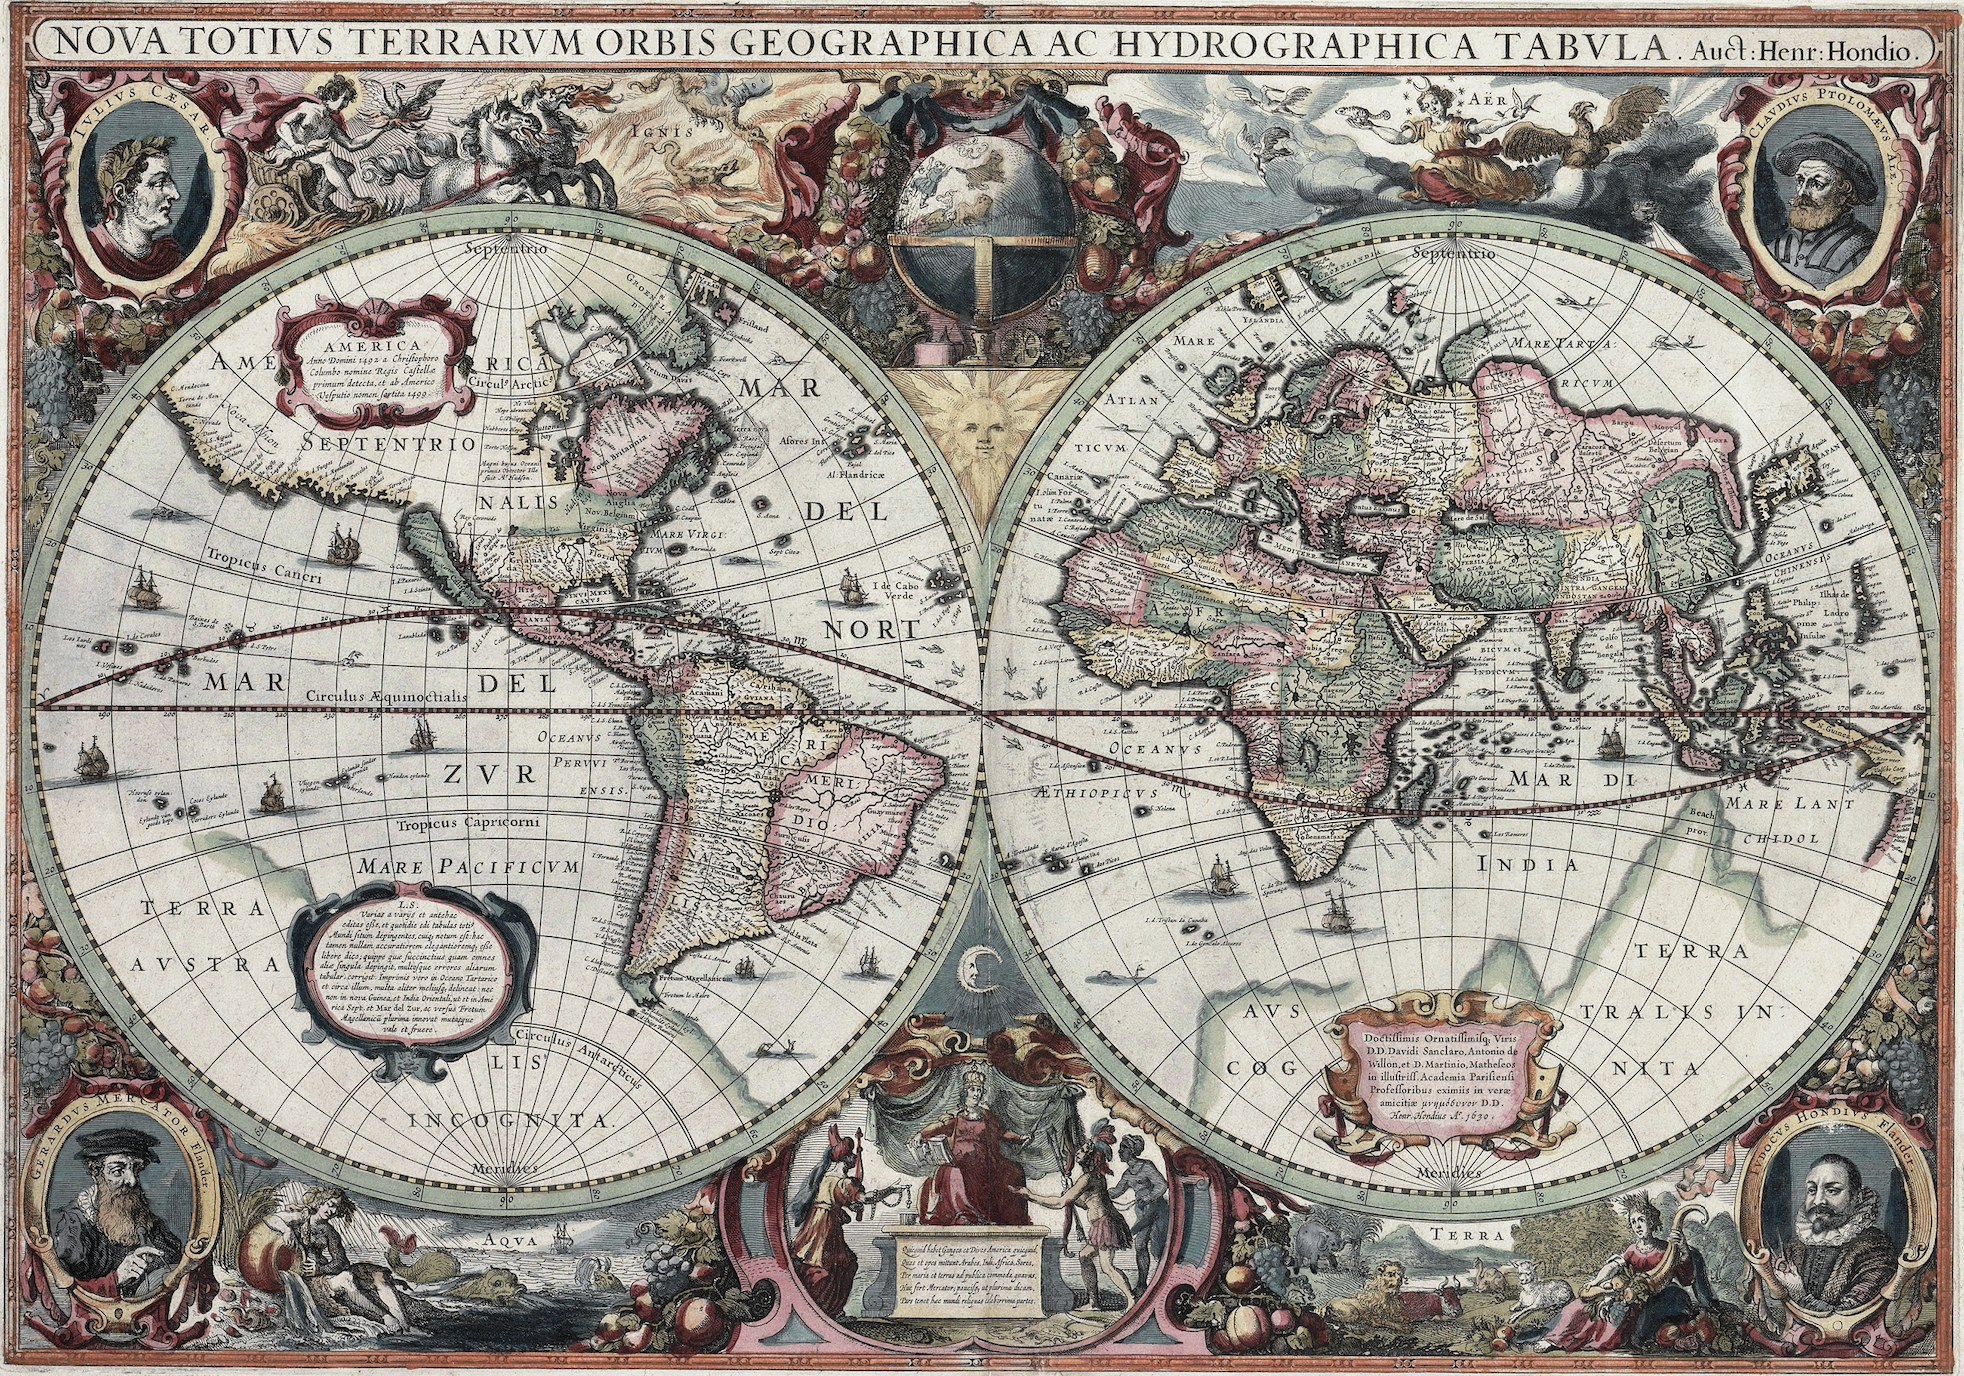
\includegraphics[scale=0.44]{./Bilder/Hondius_gesamt.png}\\[0.2cm]
\includegraphics[scale=0.2]{./Bilder/Hondius_00.jpg} \hfill
\includegraphics[scale=0.31]{./Bilder/Hondius_90.jpg}
\caption{\label{fig_Hondius}%
(Oben) Weltkarte von Hendrik Hondius aus dem Jahr 1630. Deutlich erkennbar neben der
\"Aquatorlinie ist die Projektion der Ekliptik. (Unten)
Ausschnitte aus der Weltkarte von Hendrik Hondius. (links) Ausschnitt beim Schnittpunkt von 
\"Aquator und Ekliptik, der hier auf einen der damals gebr\"auchlichen Nullmeridiane durch die
Azoren gelegt wurde. Links unten sind Teile von S\"udamerika erkennbar, rechts oben Teile von
Afrika. (rechts) Ausschnitt in der N\"ahe des s\"udlichen Wendepunkts der Ekliptik (unser
Winterpunkt). Der Kontinent links ist Afrika, die Insel rechts daneben Madagaskar; rechts oben
erkennt man die S\"udspitze von Indien und Sri Lanka (damals Ceylon). (\cite{Puzzle})}
\end{figure}

Sowohl die \"Aquatorlinie als auch die Ekliptik sind in $360$ \"aquidistante Einheiten von
jeweils $1^\circ$ unterteilt. F\"ur die \"Aquatorlinie gilt das auch auf der Karte. Da der Gro\ss kreis
der Ekliptik in seiner Projektion auf der Karte bei unterschiedlichen Breitengraden verl\"auft und
der Ma\ss stab der Karte vom Breitengrad abh\"angt (siehe auch Kap.\ \ref{chap_Landkarte}),
erscheint die Unterteilung der Ekliptik nicht mehr gleichf\"ormig.
In der N\"ahe der Wendepunkten der Sonne, also in den Bereichen, wo die
Ekliptik in der N\"ahe des $\pm 23,5$.\ Breitengrads ist, sind die Unterteilungen auf der Ekliptik etwas
breiter als am \"Aquator (siehe Abb.\ \ref{fig_Hondius}, unten rechts), da der Ma\ss stab auf der Karte kleiner
wird, wenn man sich vom \"Aquator entfernt. In den Ausschnitten (Abb.\ \ref{fig_Hondius}, unten)
erkennt man, dass beim Schnittpunkt der Ekliptik mit dem \"Aquator (also den \"Aquinoktien) die
Projektion der Ekliptik auf den \"Aquator die Bogenl\"ange schrumpfen l\"asst (Abb.\ \ref{fig_Hondius}, unten links).
An diesen Stellen schneidet die $10^\circ$ Bogenl\"ange der Ekliptik den \"Aquator links von der
$10^\circ$ Marke bzw.\ dem 10.\ L\"angengrad. Andererseits vergr\"o\ss ert
wegen des ver\"anderten Ma\ss stabs die Projektion entlang der L\"angengrade in der
N\"ahe der Wendepunkte die Bogenl\"ange (Abb.\ \ref{fig_Hondius}, unten rechts): Hier liegt die
$10^\circ$ Marke der Ekliptik ($10^\circ$ neben dem Wendepunkt) rechts neben dem 100.\ L\"angengrad
(der 90.\ L\"angengrad markiert den Wendepunkt) am \"Aquator. 

\subsection{Das Analemma}
\label{sec_Analemma}

Das Analemma\index{Analemma} 
ist eine achtf\"ormige Figur, die ungef\"ahr den Schattenverlauf der Spitze
eines Stabes (z.B.\ eines Obelisken oder der Spitze des Zeigers einer Sonnenuhr) zur
selben mittleren Ortszeit (z.B.\ um 12 Uhr mittags) im Verlauf eines Jahres beschreibt (siehe
Abb.\ \ref{fig_Analemma}, links). 
Die beiden Koordinaten dieser Figur entsprechen einmal dem unterschiedlichen H\"ochstand
der Sonne im Sommer und Winter: Im Winter steht die Sonne auch zur Mittagszeit sehr tief
und somit ist der Schatten vergleichsweise lang, im Sommer steht die Sonne hoch am
Himmel und daher ist der Schatten entsprechend kurz. 

\begin{figure}[htb]
\includegraphics[scale=0.28]{./Bilder/Analemma.jpg} 
\hfill
\includegraphics[scale=0.24]{./Bilder/Munich_Altes_Rathaus_Sundial.jpg}
\caption{\label{fig_Analemma}%
Das Analemma. (links) Die derzeitige Figur des Analemmas. Die obere Spitze der 8
beschreibt den Sonnenstand im Sommer, wenn die Sonne hoch steht und der Schatten
entsprechend kurz ist. Der Zeiger oder Obelisk steht oberhalb der Figur und die S\"udrichtung
ist nach oben (aus \cite{Wikipedia_Analemma}). (rechts) Die Sonnenuhr am Alten Rathaus in M\"unchen
mit einem Analemma zur 
Korrektur der wahren Sonnenzeit auf die mittlere Sonnenzeit. (aus \cite{Niermann})} 
\end{figure}

Die dazu (fast) orthogonale Richtung entspricht der Zeitgleichung: Da die Position der Schattenspitze
immer zur selben mittleren Ortszeit bestimmt wird, geht die wahre Sonne dieser Zeit entsprechend
der Zeitgleichung entweder etwas vor oder nach, d.h.\ der Schatten ist etwas nach links oder
rechts versetzt. 

Manche Sonnenuhren korrigieren den Effekt der Zeitgleichung. Dazu gibt es unterschiedliche
Verfahren. Man kann z.B.\ die Schattenlinien zu einer festen Uhrzeit nicht als Geraden zeichnen
(die einem festen L\"angengrad entsprechen w\"urden) sondern in Form einer langgestreckten
Acht. Hierbei wird, wie bei all diesen Verfahren, ausgenutzt, dass der Schatten im Winter l\"anger
ist als im Sommer. 

Ein weiteres Verfahren besteht darin, den Schattenstab der Sonnenuhr unterschiedlich dick
zu machen und zum Ablesen an einer Skala eine bestimmte Kante des Schattens zu 
verwenden (siehe Abb.\ \ref{fig_Bernhardt}).
Solche St\"abe bezeichnet man auch als Bernhardt'sche Walze (benannt nach dem Techniker
Martin Bernhardt,\index{Bernhardt'sche Walze} 
der diese Walze patentieren lie\ss, \"ahnliche Ideen hatte aber auch schon
der Engl\"ander John Ryder Oliver Ende des 19.\ Jahrhunderts). 
Ebenfalls wegen der unterschiedlichen Sonnenh\"ohe zu den verschiedenen Jahreszeiten
w\"urde ein jeweils anderer Teil des Schattenstabs den Schatten auf die Skala werfen. Wegen
der unterschiedlichen Dicke erreicht man so, dass diese Schattenkante entsprechend 
verschoben ist. Da die Zeitgleichung in den beiden Jahresh\"alften unterschiedlich ist, ben\"otigt
man einen Schattenstab f\"ur die erste und einen anderen Schattenstab f\"ur die zweite
Jahresh\"alfte.   

\begin{SCfigure}[30][h]
\includegraphics[scale=0.2]{./Bilder/Bernhardt.jpg}
\caption{\label{fig_Bernhardt}%
Sonnenuhr mit Bernhardt'scher Winterwalze. (aus \cite{Wikipedia_Sonnenuhr})}
\end{SCfigure}

Im Verlauf der Zeit verschieben sich die beiden Beitr\"age zur Zeitgleichung gegeneinander. 
W\"ahrend sich der Neigungswinkel zur Ekliptik nur sehr wenig und \"uber einen sehr gro\ss en
Zeitraum von \"uber 40\,000 Jahren ver\"andert, wandert das Perihel im Verlauf von rund 
21\,000 Jahren einmal durch das Jahr. Dadurch ver\"andert sich die Zeitgleichung langsam
und somit auch die Form des Analemmas. Derzeit ist das Analemma leicht asymmetrisch,
weil die Wintersonnenwende und das Perihel nicht auf denselben Tag fallen (das war z.B.\ im
Jahr 1246 der Fall). Au\ss erdem sind die beiden \glqq Hanteln\grqq\ der Acht unterschiedlich 
gro\ss. Wenn das Perihel im Fr\"uhlings- bzw.\ Herbstpunkt steht, sind die beiden Teile
gleich gro\ss.  

\subsection{Der k\"urzeste Tag}

Die Wintersonnenwende entspricht gemeinhin dem k\"urzesten Tag. Derzeit liegt dieses Ereignis
um den 21.\ Dezember.\index{Wintersonnenwende} 
Zu diesem Zeitpunkt befindet sich sie Sonne \"uber dem s\"udlichen
Wendekreis (dem Wendekreis des Steinbocks).\index{Wendekreis des Steinbocks} 
In Freiburg liegen zwischen Sonnenaufgang\index{Freiburg!Sonnenauf-,-untergang}
und Sonnenuntergang an diesem Tag 8 Stunden, 22 Minuten und 13 Sekunden. Doch k\"urzester 
Tag hei\ss t nicht, dass es an diesem Tag am fr\"uhesten dunkel wird oder am sp\"atesten
hell. Der fr\"uheste Sonnenuntergang liegt um den 11.\ Dezember (in Freiburg um 16:35),
der sp\"ateste Sonnenaufgang ist um den 2.\ Januar (in Freiburg gegen 8:18). Alle angegebenen
Uhrzeiten beziehen sich nat\"urlich auf die mittlere Sonnenzeit (genauer MEZ) und nicht die
wahre Sonnenzeit. Der Grund f\"ur den Unterschied ist die Zeitgleichung. 

Eine \"ahnliche Aussage gilt f\"ur die Sommersonnenwende.\index{Sommersonnenwende} 
Der l\"angste Tag mit
16 Stunden 2 Minuten und 47 Sekunden in Freiburg ist der 21.\ Juni. Doch der fr\"uhste Sonnenaufgang
liegt um den 16./17.\ Juni (gegen 5:18), der sp\"ateste Sonnenuntergang um den 25./25.\ Juni (gegen
21:32). Genaue Zeiten f\"ur die Tagesl\"ange, Sonnenauf- und Untergang sowie weitere
interessante Daten f\"ur jeden beliebigen Ort der Erde findet man auf der Webseite \cite{timeanddate}.

\section{Anhang}
\subsection{\"Aquivalenz des zweiten Kepler'schen Gesetzes und der Drehimpulserhaltung}
\label{sec_Zeitgleichung_A}

Sei $\pmb{r}$ der Verbindungsvektor von einem Brennpunkt der Ellipse - dem Brennpunkt, in 
dem sich die Sonne befindet - zu einem Punkt auf der Ellipse (dem Ort eines Planeten)
und $\Delta \pmb{r}$ die in der Zeit $\Delta t$ zur\"uckgelegte Strecke in tangentialer
Richtung. Das zweite Kepler'sche Gesetz\index{Kepler'sches Gesetz!zweites} 
besagt, dass die in dem Zeitraum $\Delta t$ (f\"ur $\Delta t\rightarrow 0$)
\"uberstrichene Fl\"ache $\Delta F$, d.h.
\begin{equation}
                    \Delta F = \frac{1}{2} \pmb{r} \times \Delta \pmb{r} \, ,
\end{equation} 
entlang der Bahnkurve immer gleich ist. Damit ist aber auch der Drehimpuls
\begin{equation}
                    \pmb{L} = m  \pmb{r} \times \frac{{\rm d} \pmb{r}}{{\rm d} t} 
\end{equation} 
konstant.\index{Drehimpulserhaltung}
Das Argument gilt nat\"urlich auch in der umgekehrten Richtung: Aus der
Drehimpulserhaltung folgt das zweite Kepler'sche Gesetz.


\begin{thebibliography}{99}
\bibitem{Wikipedia_Analemma} aus Wikipedia \glqq Analemma\grqq; S.\ Wetzel, CC BY-SA 4.0.
\bibitem{Niermann} Till Niermann - Eigenes Werk, CC BY-SA 3.0, 
                \url{https://commons.wikimedia.org/w/index.php?curid=21792620}
\bibitem{Puzzle} Ravensburger Puzzle; Antique World Map, Hondius.                 
\bibitem{timeanddate} 
   {\small \verb+https://www.timeanddate.com/sun/germany/freiburg+} 
\bibitem{Wikipedia_Sonnenuhr} Wikipedia \glqq Sonnenuhr\grqq; 
           Pr\"azisions-Sonnenuhr mit Winterwalze am Carl Zeiss Planetarium, Stuttgart.
           \url{https://de.wikipedia.org/wiki/Sonnenuhr}   
\bibitem{Wikipedia_Zeitgleichung} Wikipedia \glqq Zeitgleichung\grqq; 
                 \url{https://de.wikipedia.org/wiki/Zeitgleichung} (aufgerufen am 14.5.2023).
\bibitem{Wikipedia_Zeitzone} Wikipedia \glqq Zeitzone\grqq. \url{https://de.wikipedia.org/wiki/Zeitzone}
\end{thebibliography}


\end{document}


%\documentclass[german,10pt]{book}      
\usepackage{makeidx}
\usepackage{babel}            % Sprachunterstuetzung
\usepackage{amsmath}          % AMS "Grundpaket"
\usepackage{amssymb,amsfonts,amsthm,amscd} 
\usepackage{mathrsfs}
\usepackage{rotating}
\usepackage{sidecap}
\usepackage{graphicx}
\usepackage{color}
\usepackage{fancybox}
\usepackage{tikz}
\usetikzlibrary{arrows,snakes,backgrounds}
\usepackage{hyperref}
\hypersetup{colorlinks=true,
                    linkcolor=blue,
                    filecolor=magenta,
                    urlcolor=cyan,
                    pdftitle={Overleaf Example},
                    pdfpagemode=FullScreen,}
%\newcommand{\hyperref}[1]{\ref{#1}}
%
\definecolor{Gray}{gray}{0.80}
\DeclareMathSymbol{,}{\mathord}{letters}{"3B}
%
\newcounter{num}
\renewcommand{\thenum}{\arabic{num}}
\newenvironment{anmerkungen}
   {\begin{list}{(\thenum)}{%
   \usecounter{num}%
   \leftmargin0pt
   \itemindent5pt
   \topsep0pt
   \labelwidth0pt}%
   }{\end{list}}
%
\renewcommand{\arraystretch}{1.15}                % in Formeln und Tabellen   
\renewcommand{\baselinestretch}{1.15}                 % 1.15 facher
                                                      % Zeilenabst.
\newcommand{\Anmerkung}[1]{{\begin{footnotesize}#1 \end{footnotesize}}\\[0.2cm]}
\newcommand{\comment}[1]{}
\setlength{\parindent}{0em}           % Nicht einruecken am Anfang der Zeile 

\setlength{\textwidth}{15.4cm}
\setlength{\textheight}{23.0cm}
\setlength{\oddsidemargin}{1.0mm} 
\setlength{\evensidemargin}{-6.5mm}
\setlength{\topmargin}{-10mm} 
\setlength{\headheight}{0mm}
\newcommand{\identity}{{\bf 1}}
%
\newcommand{\vs}{\vspace{0.3cm}}
\newcommand{\noi}{\noindent}
\newcommand{\leer}{}

\newcommand{\engl}[1]{[\textit{#1}]}
\parindent 1.2cm
\sloppy

         \begin{document}  \setcounter{chapter}{3}


\chapter{Zeitsysteme}
% Kap 4
\label{chap_Zeitsysteme}

\info{Thomas Filk}{28.03.2024}%
Seit 1967 ist die Sekunde\index{Sekunde} 
durch die Frequenz $\Delta \nu_{\rm Cs}$ des Hyperfeinstruktur\"ubergangs\index{Hyperfeinstruktur\"ubergang}
in 133-C\"asium im Grundzustand definiert. Es gilt:
\begin{equation}
               1\,{\rm s}  =  9\,192\,631\,770 \, T = 9\,192\,631\,770 \, \frac{1}{\Delta \nu_{\rm Cs}} \, .
\end{equation}  
$T$ ist die Periodenl\"ange einer Schwingung zu diesem \"Ubergang.
Die Definition der Sekunde \"uber den Hyperfeinstruktur\"ubergang in 133-C\"asium l\"oste 1967 die 
Ephemeridensekunde ab, die \"uber die Position der Erde relativ zur Sonne definiert 
war.\index{Zeitsysteme|(} 

Man k\"onnte meinen, dass mit der Definition der SI-Sekunde und der Konstruktion von
Uhren, die diese Sekunde genau genug messen k\"onnen, das Problem der Zeitmessung
gel\"ost sei. Im Detail ergeben sich jedoch Probleme, die zu verschiedenen
Zeitsystemen gef\"uhrt haben. Zum einen muss man zwischen theoretischen Zeitsystemen,
die auf idealen Uhren basieren, und den Realisierungen solcher Zeitsysteme durch
tats\"achlich existierende und mit Fehlern behaftete Uhren unterscheiden. In diesem Zusammenhang
ist zu definieren, wie man aus den fehlerbehafteten Werten realer Messinstrumente eine Zeitskala
definiert kann. Au\ss erdem muss
man einen Referenzpunkt w\"ahlen, da nach der speziellen und allgemeinen Relativit\"atstheorie
Uhren an verschiedenen Orten (im Gravitationsfeld) oder in verschiedenen Bewegungszust\"anden
unterschiedliche Zeitsysteme definieren. Und schlie\ss lich m\"ochte man nat\"urlich, dass die
Zeitsysteme trotz ihrer derzeitigen Definition \"uber atomare Eigenschaften noch etwas mit dem 
Tag-und-Nacht-Rhythmus der Erde zu tun haben.

Auch heute noch sind verschiedene Zeitsysteme in Gebrauch. Die folgende Liste bzw.\ Behandlung
dieser Zeitsysteme kann daher nur einen groben \"Uberblick geben. 

\section{Das Julianische Datum}

Die Julianische Tagesz\"ahlung (englisch \textit{Julian day}) z\"ahlt, unabh\"angig von einem 
speziellen Kalender oder der Definition eines Jahres,\index{Julianische Tagesz\"ahlung}
die Tage seit einem Anfangsdatum, das als der 1.\ Januar des Jahres 4713 v.\,Chr.\ nach dem
zur\"uckextrapolierten Julianischen Kalender gew\"ahlt wird. Genauer beginnt diese Z\"ahlung mittags
um 12 Uhr (Sonnenh\"ochstand am heutigen Nullmeridian durch Greenwich). W\"ahlt man nicht den
zur\"uckgerechneten Julianischen Kalender sondern den zur\"uckgerechneten Gregorianischen
Kalender, so beginnt diese Zeitrechnung mit dem 24.\ November des Jahres 4714 v.\,Chr. Und da es
weder im Julianischen noch im Gregorianischen Kalender das Jahr 0 gibt, entspricht das Jahr 4713 dem
Jahr $-$4712 im astronomischen Kalender, der das Jahr 0 hinzunimmt. 

Die Wahl dieses Datums hat historische Gr\"unde. Zun\"achst werden hier drei Zyklen zu einer
Epoche zusammengefasst: Der Menton-Zyklus\index{Menton-Zyklus} 
oder Mondzyklus von 19 Jahren, der Sonnenzyklus\index{Sonnenzyklus}
von 28 Jahren\footnote{Im Julianischen Kalender haben 4 Jahre - die Periode dieser Kalenderz\"ahlung - 
eine Dauer von 1461 Tagen, dabei verschieben
sich die Wochentage um 5 Tage - der Rest bei einer Teilung von 1461 durch 7. 
Alle $4\times 7=28$ Jahre fallen also die Wochentage wieder auf dasselbe Datum. Im
Gregorianischen Kalender entspricht eine Periode 400 Jahren mit 146\,097 Tagen. Dies ist glatt durch 7 teilbar,
d.h.\ alle 400 Jahre fallen im Gregorianischen Kalender dieselben Daten wieder auf dieselben Wochentage.}
und der sogenannte Indiktionszyklus\index{Indiktionszyklus} 
von 15 Jahren (ein Zyklus, der im Altertum und Mittelalter
oft verwendet wurde und urspr\"unglich mit Neuberechnungen der Steuern einherging). 
Das Produkt dieser drei Zyklenl\"angen sind
7980 Jahre; dies bezeichnet man als eine Epoche. Das Jahr 4713 v.Chr.\ wurde im Mittelalter errechnet
als ein Jahr, in dem alle drei genannten Zyklen nach damaliger Rechnung begannen. Es hat den Vorteil, dass
es vor jeder historischen Datierung liegt, d.h.\ es gibt keine datierten historischen Ereignisse vor diesem
Jahr (au\ss er astronomische Ereignisse, die man heute zur\"uckrechnen kann). 

Dem Julianische Tag, der am 1.\ Januar 2000 mittags 12 Uhr (Universal time im Gregorianischen Kalender) begann, 
entspricht nach der Julianischen Tagesz\"ahlung  der Tag 2\,451\,545. Soviel Tage sind seit dem 1.\ Januar 4713 v.\,Chr.\
nach dem zur\"uckgerechneten Julianischen Kalender vergangen. Diese Z\"ahlung ist so einfach, dass
sie nicht nur in der Astronomie gerne verwendet wird, sondern auch in abgewandelter
Form in vielen Computersystemen. 

Will man neben dem Tag auch die Uhrzeit ber\"ucksichtigen, werden Nachkommastellen angegeben.
Der Tag hat 86\,400 Sekunden, sodass der 1.\ Januar 2000, 22 Uhr 25 Minuten und 10 Sekunden dem
Julianischen Datum 2\,451\,545,43414 entspricht. Sowohl die Julianische Tagesz\"ahlung (im Englischen
\textit{Julian Day}) als auch das\index{Julianisches Datum}  
Julianische Datum (\textit{Julian Date}) werden mit JD abgek\"urzt. 
Man beachte, dass diese Tagesz\"ahlung abgesehen von der Angabe des Anfangsdatums
nicht davon abh\"angt, ob ansonsten der Julianische oder Gregorianische Kalender (oder welcher andere 
Kalender auch immer) verwendet wird. 

Eine h\"aufig verwendete Abwandlung ist das sogenannte\index{Julianisches Datum!Modfiziertes} 
Modifizierte Julianische Datum, abgek\"urzt mit
MJD. Dies wird beispielsweise auch von dem BIPM (Bureau International des Poids et Mesures) in seinen
\textit{Circular T},\index{Circular T}\index{BIPM, Bureau International des Poids et Mesures} 
den monatlichen Berichten zur Bestimmung der Internationalen Atomzeit TAI,
verwendet. Das MJD unterscheidet sich vom JD in zwei Punkten:
\begin{enumerate}
\item
Der Tagesanfang wird auf 0 Uhr Mitternacht (statt auf 12 Uhr mittags) gelegt.
\item  
Der Beginn ist 0 Uhr, 17.\ November 1858. Das bedeutet, vom Julianischen Tag werden 2\,400\,000,5 Tage
abgezogen: ${\rm MJD=JD}-2\,400\,000,5$.       
\end{enumerate}
Damit hat der 1.\ Januar 2000, 12 Uhr mittags, den Wert: ${\rm MJD}= 51\,544,5$.  

\section{Die Ephemeridenzeit - ET}

Die\index{Ephemeridenzeit} 
Sekunde als der 1/86\,400-ste Teil eines Tages ist erst seit dem Mittelalter in Gebrauch
und bis 1956 war die Sekunde als der 1/86\,400-ste Teil eines mittleren Sonnentages definiert. 
Man wusste zu diesem Zeitpunkt allerdings schon, dass auch der mittlere Sonnentag nicht wirklich
vollkommen gleichm\"a\ss ig verl\"auft bzw.\ dass der mittlere Sonnentag davon abh\"angt, \"uber
welchen Zeitraum genau gemittelt wird. Daher verwendete man schon seit l\"angerem die Stellung
der Erde relativ zur Sonne zur Definition einer Sekunde. So war in der Zeit zwischen 1956 und 1968
die Sekunde definiert als der 1/31\,556\,925,9747-ste Teil des tropischen Jahres 1900 
(genauer: des theoretisch hochgerechneten tropischen
Jahres 1900, bestimmt aus den Bahndaten der Erde zum Zeitpunkt 31.12.1899, mittags 12 Uhr).
Diese Definition der Sekunde bezeichnet man auch als die 
Ephemeridensekunde.\index{Ephemeridensekunde}

Schon in babylonischer Zeit (um 1000 v.\,Chr.) gab es Tabellen zu den Positionen von Sonne, Mond und
Planeten, und der sogenannte\index{Almagest (Ptolem\"aus)} 
Almagest von Ptolem\"aus mit seinen genauen Beschreibungen der
Planetenbahnen gilt als H\"ohepunkt antiker Astronomie. Im Mittelalter wurden weitere 
Tabellen\index{Ephemeridentabellen} 
erstellt (bekannt sind die Toledaner Tafeln aus dem 12.\ Jahrhundert, die Alfonsinischen Tafeln 
aus dem 13.\ Jahrhundert, die Ephemeridentafeln von Regiomontanus von 1474, oder 
auch die Rudolfinischen Tafeln von 1627 von Johannes Kepler).  
  
Seit dem Mittelalter gab es Tabellen, in denen die Position der Sonne, des Mondes und der Planeten
relativ zu einem Koordinatensystem (meist durch Angabe der Rektazension und Deklination) 
und/oder relativ zueinander mit Daten und Tageszeiten korreliert wurden. 

\section{TT, TCG und TCB}
 
TT (\textit{Terrestial Time} oder \textit{Temps terrestre}), TCG (\textit{Geocentric Coordinated Time} oder
\textit{Temps-coordonn\'{e}e geocentrique}) und TCB (\textit{Barycentric Coordinate Time} oder
\textit{Temps-coordonn\'{e}e barycentrique}) sind idealisierte Zeitsysteme, manchmal spricht man auch von
Platonischen Zeitsystemen,\index{Zeitsystem!Platonisches} 
die auf idealen Uhren unabh\"angig von konkreten Realisierungen beruhen.
Sie dienen meist der theoretischen Beschreibung von Objekten in unserem Sonnensystem. 

TCB (baryzentrische koordinierte Zeit)\index{TCB, baryzentrisch koordinierte Zeit} 
ist die Zeit einer idealen, die SI-Sekunde anzeigenden Uhr, 
die sich in einem idealisierten hypothetischen 
System befindet, das sich parallel zum Schwerpunkt (dem Baryzentrum) des Sonnensystems bewegt,
also dieselben Bewegungen wie dieser Schwerpunkt ausf\"uhrt, aber keinem Gravitationspotenzial
unterliegt. Es wird typischerweise f\"ur die Beschreibung von Bahnkurven von Planeten oder Kometen
verwendet sowie von Raketen oder Satelliten, die den gravitativen Einfluss der Erde verlassen. 
Entsprechend ist\index{TCG, geozentrisch koordinierte Zeit} 
TCG (geozentrische koordinierte Zeit) die Zeit einer idealen, die SI-Sekunde anzeigenden 
Uhr, die sich in einem idealisierten System befindet, das sich parallel zum Schwerpunkt des Erdmittelpunkts 
bewegt, aber keinem Gravitationspotenzial unterliegt. Sie dient zur Beschreibung von Bahnkurven im 
gravitativen Einfluss der Erde, beispielsweise den Bahnkurven von Satelliten, dem Mond oder Raketen. 

TT (terrestrische Zeit)\index{TT, terrestrische Zeit} 
ist die Zeit einer idealen Uhr, die sich auf der Oberfl\"ache der Erde befindet. Hierbei ist die Oberfl\"ache
definiert durch die gravitative \"Aquipotentialfl\"ache (also konstantes Gravitationspotenzial) zur mittleren 
Meeresh\"ohe, wobei der Effekt der Erddrehung (Potenzial zur Fliehkraft) 
einbezogen wird, nicht jedoch der Einfluss von Str\"omungen oder Gezeiten. Diese Fl\"ache bezeichnet man
auch als das Geoid der Erde. Da die mittlere Meeresh\"ohe\index{Meeresh\"ohe, mittlere}
(z.B.\ im Zusammenhang mit dem Klimawandel) keine Konstante ist, hat man f\"ur das Potenzial
den Wert $U/c^2=6,969\,290\,134\cdot 10^{-10}$ definiert (der Quotient aus einem Potenzial
und $c^2$ ist eine dimensionslose Konstante), was bei einer homogenen Kugel von der Masse der Erde
einem Radius von etwas \"uber 6\,360\,km entspricht. 

TT und TCG unterscheiden sich also um einen multiplikativen Faktor $( 1 - U/c^2)$, um den TT langsamer
ist als TCG. Au\ss erdem wurde definiert, dass die beiden Zeiten am 1.\ Januar 1977, um 0 Uhr 32,184 Sekunden,
gleich waren. Die seltsame Sekundenzahl ergibt sich daraus, dass TT m\"oglichst exakt an die vorher
gebr\"auchliche Ephemeridenzeit angepasst werden sollte. Au\ss erdem entspricht diese Zeit exakt 0 Uhr nach 
der Internationalen Atomzeit TAI (siehe n\"achsten Abschnitt). Fr\"uher verwendete man f\"ur die terrestrische
Zeit TT die Bezeichnung TDT\index{TDT, terrestrial dynamical time} 
(terrestrial dynamical time); diese Bezeichnung findet man gelegentlich immer noch.  

\section{Die Internationale Atomzeit - TAI}

Die Internationale Atomzeit TAI\index{TAI, internationale Atomzeit} 
(\textit{Temps atomique international}) ist eine Realisierung von TT. Hierbei
handelt es sich um eine Zeit, die an existierenden Uhren abgelesen wird. Da eine einzelne Uhr immer
ungenau ist und auch mal St\"orungen haben kann, handelt es sich bei TAI um einen gewichteten
Mittelwert von derzeit \"uber 400 hoch pr\"azisen Uhren an \"uber 80 Orten. In der Physikalisch Technischen
Bundesanstalt (PTB)\index{PTB, Physikalisch Technische Bundesanstalt} 
in Braunschweig stehen zwei solche Atomuhren - genannt CSF1 und CSF2, hierbei handelt
es sich um C\"asium Fountain Clocks -, die zur
TAI beitragen. In regelm\"assigen Abst\"anden \"ubermitteln diese Uhren ihre Zeiten an das
BIPM. Dort werden die Daten um verschiedene Faktoren korrigiert (dazu z\"ahlen Laufzeiten der \"Ubertragung
sowie relativistische Korrekturen aufgrund der H\"ohenunterschiede der verschiedenen Uhren), die
Uhren mit den gr\"o\ss ten Abweichungen werden nicht ber\"ucksichtigt und von rund 300 Uhren wird
ein gewichtetes Mittel gebildet. Die Gewichtung der einzelnen Uhren richtet sich nach ihrem gesch\"atzten 
Fehler (der sich aus einer Theorie ihrer Funktionsweise bestimmt) sowie Ungenauigkeiten oder
Schwankungen in der Vergangenheit. Einmal im Monat wird im
\textit{BIPM Circular T} ver\"offentlicht, um wie viel die einzelnen Uhren von dem berechneten Mittelwert
zu bestimmten Zeitpunkten (die dann rund einen Monat zur\"uckliegen) abwichen. 

TAI versucht also eine m\"oglichst genaue Realisation einer idealen, die SI-Sekunde anzeigenden Uhr
zu sein, die sich auf der Oberfl\"ache des Geoids befindet. 
Insofern ist sie eine Realisation von TT, bis auf die oben erw\"ahnten 32,184 Sekunden, um die
sich die beiden Zeiten am 1.\ Januar 1977, 0 Uhr (TAI-Zeit), unterschieden. TT sollte dabei an die Ephemeridenzeit
angepasst werden, an die TAI schon 1958 angepasst worden war. Die 32,184 Sekunden Unterschied
erkl\"aren sich also daher, dass zwischen diesen beiden Zeitpunkten (1958 und 1977) schon ein
solcher Unterschied zwischen der Atomzeit und der Ephemeridenzeit bestand. 

\section{Universal Times - UT0, UT1, UT2}

Die\index{UT, Universal Times} 
Universal Times beziehen sich direkt auf die Lage der Erde und sind somit eine Fortf\"uhrung
der Ephemeridenzeit. Die Universal Time ist definiert \"uber den Winkel, den der Nullmeridian auf der
Erde relativ zu einem ausgezeichneten Punkt auf dem Himmels\"aquator (der Projektion des Erd\"aquators
vom Mittelpunkt der Erde aus auf die Himmelskugel) hat. Dieser Punkt auf dem Himmels\"aquator
ist heute definiert \"uber ein Referenzsystem am Himmel, das \"uber die Lage von festen Punkten am
Himmel - meist Quasare, die auch im Radiowellenbereich nachweisbar sind, sodass eine VLBI (Very Long
Baseline Interferometry) eine sehr genaue Richtungsbestimmung auch am Tag erm\"oglicht - definiert ist. Dieses
Referenzsystem bezeichnet\index{ICRF, International Celestial Reference Frame} 
man auch als ICRF (\textit{International Celestial Reference Frame}).   

Die Ephemeridenzeit bezog sich auf einen gemittelten Tag, wie er durch das (vom 31.12.1899, 12 Uhr, hochgerechnete) Jahr 1900 definiert war.\index{GMT, Greenwich Mean Time} 
Diese Zeit nannte man auch GMT (\textit{Greenwich Mean Time}). Sie entspricht genau
dem, was man sp\"ater UT0 nannte: Eine Zeitbestimmung \"uber einen gemittelten Sonnentag, also die Zeit
eines realen Sonnentags, die durch die Zeitgleichung - also die Einfl\"usse der elliptische Bahn der Erde sowie ihrer Neigung
gegen\"uber der Ekliptik - korrigiert wird und somit zur Zeit eines mittleren Sonnentags geh\"ort. 
Der Winkel ERA (\textit{Earth Rotation Angle})\index{ERA, Earth Rotation Angle} 
des Nullmeridians relativ zu dem Referenzsystem am Himmel  
ist bis auf eine Konstante direkt proportional zur UT. Die Proportionalit\"atskonstante ber\"ucksichtigt, dass es sich
hierbei um eine Messung der Erdrotation relativ zu einem Himmelssystem (siderischen Referenzsystem)
handelt, und diese Zeit korrigiert werden muss, um einen Sonnentag zu erhalten. Dementsprechend entspricht
dieser Proportionalit\"atsfaktor ziemlich genau dem Faktor $(1+1/365,25)$, um den der siderische Tag im 
Vergleich zum Sonnentag korrigiert werden muss. Genauer lautet die Beziehung:
\begin{equation}
      {\rm ERA} = 2\pi (0,7790572732640 + 1,00273781191135448 \cdot T_{\rm u}) \, {\rm rad}  \, ,
\end{equation}
wobei $T_{\rm u} = ({\rm JD(UT1)} - 2\,451\,545,0)$ ist, und ${\rm JD(UT1)}$ dem Julianischen Datum
nach der UT1-Uhrzeit entspricht. ERA ist die gemessene Variable (ein Winkel) und JD(UT1) - ein Datum
mit einem Zeitpunkt - wird daraus berechnet. ERA, also der gemessene Winkel, wird dabei um zwei
Faktoren korrigiert: (1) die Zeitgleichung, die den Unterschied zwischen mittlerem und wahrem 
Sonnentag angibt, und (2) Schwankungen in der Drehachse der Erde (sogenannte Polarbewegungen), durch die
der L\"angengrad, beispielsweise eines Observatoriums, nicht eindeutig bestimmt ist. Weitere jahreszeitliche
Schwankungen, die beispielsweise in dem Zeitsystem UT2 ber\"ucksichtigt werden, werden f\"ur UT1 nicht
ber\"ucksichtigt.       

\section{Universal Coordinated Time - UTC}

Wir haben nun zwei realisierte Zeitsysteme (d.h., Zeitsysteme, die durch Messungen an realen physikalischen Systemen bestimmt werden): 
Die TAI, die \"uber Atomuhren bestimmt wird, die m\"oglichst nahe an der SI-Sekunde
arbeiten, und UT1, die \"uber die Lage der Erde relativ zur Sonne bestimmt wird. UT1 hat den Vorteil, dass 12 Uhr
mittags mit unserer Vorstellung von \glqq Sonnenh\"ochststand\grqq\ zusammenf\"allt, wohingegen TAI auf einer
m\"oglichst genauen und gleichm\"a\ss igen Realisierung einer Sekunde beruht. Damit entsteht das Problem:
An welches Zeitsystem sollen wir uns halten, wenn diese beiden Zeitsysteme auseinanderlaufen. UT1 hat den Vorteil,
unseren Vorstellung von Tag und Nacht zu entsprechen, TAI hat den Vorteil, dass die Sekunden immer gleich
lang sind. 

Um ein Auseinanderlaufen der beiden Zeitsysteme auszugleichen, hat man sich (nach anf\"anglichen Problemen bei
der Namensgebung wie auch bei der genauen Definition) 1972 auf das Zeitsystem 
der UTC\index{UTC, Universal Coordinated Time}
(\textit{Universal Coordinated Time}) geeinigt. UCT verl\"auft parallel zu TAI, d.h., UTC richtet sich bez\"uglich
der genauen Zeitangabe nach der besten Realisierung der SI-Sekunde auf der Erdoberfl\"ache, und das ist
die TAI. Bevor allerdings UT1 und TAI um 0,9 Sekunden auseinanderlaufen (weil die Erddrehung gewissen
Schwankungen unterworfen ist), wird f\"ur UTC eine\index{Schaltsekunde} 
Schaltsekunde entweder eingef\"ugt oder weggelassen.
In der Vergangenheit wurden nur Schaltsekunden eingef\"ugt, da die Erdrotation etwas langsamer ist als
die TAI-Zeit. Als UTC im Jahre 1972 eingef\"uhrt wurde bestand schon ein Unterschied von 10 Sekunden
zwischen UT1 und TAI, sodass damals definiert wurde UTC = TAI - 10\,s. Seitdem wurden insgesamt 27
weitere Schaltsekunden eingef\"ugt, die letzte am 31.\ Dezember 2016. S\"amtliche Schaltsekunden wurden
in der Vergangenheit entweder am 31.\ Juni oder am 31.\ Dezember eingef\"ugt. In den letzten Jahren hat
die Geschwindigkeit der Eigendrehung der Erde wieder etwas zugenommen, sodass nicht ausgeschlossen
wird, dass in der nahen Zukunft zum ersten Mal in der Geschichte der UTC eine Sekunde \glqq herausgenommen\grqq\ wird. 

Das Einf\"ugen von Schaltsekunden f\"uhrte dazu, dass im Zeitsystem der UTC gelegentlich eine Minute
61 Sekunden hat. Statt nach der 59.-sten Sekunde die 0.te Sekunde folgen zu lassen, z\"ahlt man 
eine 60.ste Sekunde hinzu und beginnt dann den neuen Monat mit der Sekunde 0. Da in der Vergangenheit
noch nie eine Schaltsekunde entfernt wurde, gibt es gewisse Bedenken, ob alle Computersysteme mit einem
solchen Schritt zurecht kommen. Da auch beim Einf\"ugen von Schaltsekunden in der Vergangenheit immer
wieder Probleme mit verschiedenen digitalen Systemen auftraten, wurde in j\"ungerer Zeit \"uberlegt, die
Definition von UTC nochmals zu \"andern. Es wird angestrebt, bis 2035 eine neue Definition zu finden, bei
der nur alle paar Jahrhunderte eine Korrektur notwendig wird \cite{BIPM2022}. Beispielsweise k\"onnte man die Differenz
zwischen UT1 und TAI auf mehrere Minuten anwachsen lassen, bevor Korrekturen vorgenommen werden.
Rein subjektiv werden wir als Menschen die langsame Verschiebung der Mittagsstunde ohnehin erst
bemerken, wenn sich die Differenz auf die Gr\"o\ss enordnung einer Stunde summiert hat. 

Die UTC ist die Zeit, die wir beispielsweise \"uber Funkuhren, das Radio oder Fernsehen empfangen.
Diese Zeit ist bis auf 0,9 Sekunden an die Orientierung der Erde relativ zum Referenzsystem des Himmels
angepasst, l\"auft parallel zur Atomzeit TAI, d.h.\ ist sehr regelm\"a\ss ig, hat aber den Nachteil, 
dass eine Minute gelegentlich eine Sekunde mehr oder weniger hat. Wegen der Unregelm\"a\ss igkeit
der Erddrehung k\"onnen Schaltsekunden nicht langfristig vorhergesagt werden, sondern erst in einem
Zeitraum von einem halben Jahr. 

\section{Lokalzeit - Local Time}

Die Lokalzeit\index{Lokalzeit} 
ist die Zeit, die von Radio- oder Fernsehstationen, Funkuhren bzw.\ \"offentlichen Uhren
an einem Ort angezeigt wird. Sie richtet sich nach der UTC, unterliegt also unter anderem der 
Einf\"ugung oder L\"oschung von Schaltsekunden, unterscheidet sich von der UTC aber in zweierlei
Hinsicht:
\begin{enumerate}
\item
Sie\index{Zeitzone} 
ber\"ucksichtigt die lokale Zeitzone: UTC ist die Fortsetzung der GMT (Greenwich Mean Time) und
richtet sich nach dem Nullmeridian durch Greenwich, d.h.\ nach dem L\"angengrad, wo im Jahresmittel
mittags um 12 Uhr die Sonne ihren H\"ochststand hat. Damit man an nahezu allen Orten um die Mittagszeit
den Sonnenh\"ochststand hat, wurde die Erde in Zeitzonen eingeteilt, die einseits von L\"angengraden,
andererseits aber auch von L\"andergrenzen berandet sind. Die meisten Zeitzonen unterscheiden sich
von der Zeitzone von Greenwich um ein Vielfaches einer vollen Stunde. Alle 15 L\"angengrade beginnt also rein rechnerisch
eine neue Zeitzone, wobei die meisten L\"ander (Ausnahmen sind die USA, Kanada, Russland und
Australien) nur eine Zeitzone haben, was z.B.\ f\"ur China bedeutet, dass es sich rechnerisch \"uber 
fast vier Zeitzonen erstreckt aber im gesamten Land dieselbe Zeitzone gilt. 
Es gibt aber auch einige L\"ander mit halbst\"undiger Zeitverschiebung (Iran $+3\frac{1}{2}$, Afghanistan $+4\frac{1}{2}$,
Indien $+5\frac{1}{2}$, Burma $+6\frac{1}{2}$, Zentralaustralien $+9\frac{1}{2}$) sowie   
viertelst\"undiger Zeitverschiebung (Nepal $+5\frac{3}{4}$, kleine Teile von Australien $+8\frac{3}{4}$
sowie die Chatham Islands $+10\frac{3}{4}$). 

Zentraleuropa (mit Ausnahme von Portugal und\index{MEZ, mitteleurop\"aische Zeit}
den Inselgruppen Kanaren, Madeira, Island und Azoren) verwenden die Mitteleurop\"aische Zeit (MEZ), die
sich von der UTC um +1 Stunde unterscheidet, d.h., wenn es in Greenwich 12 Uhr mittags ist, ist es in
Mitteleuropa bereits 1 Uhr mittags. 
\item
In den Sommermonaten\index{Sommerzeit} 
wechseln viele L\"ander auf die Sommerzeit. Dazu verschiebt man die Zeitzone um eine
weitere Stunde nach Osten, d.h., relativ zum Sonnenstand ist es eine Stunde sp\"ater. Damit verbunden ist etwas
l\"angere Dunkelheit am Morgen und etwas l\"angere Helligkeit am Abend. In diesem Fall spricht man in
Mitteleuropa von der\index{MESZ, Mitteleurop\"aische Sommerzeit} 
MESZ - Mitteleurop\"asische Sommerzeit, die sich von der UTC um +2 Stunden unterscheidet.      
\end{enumerate}
Ungef\"ahr entlang des 180-sten L\"angengrads (im Pazifik, durch die Fiji-Inseln) verl\"auft die Internationale Datumsgrenze.\index{Datumsgrenze}
\"Uberquert man diese Grenze von West nach Ost, muss man das Datum um einen Tag zur\"uckstellen, \"uberquert
man sie von Ost nach West stellt man das Datum um einen Tag vor. 

\section{GPS Time}

Abschlie\ss end soll noch kurz auf die GPS-Zeit\index{GPS-Zeit}\index{GPS, Global Positioning System} 
des Global Positioning Systems (GPS) eingegangen werden. 
Das GPS besteht unter anderem aus 24 aktiven Satelliten (es befinden sich derzeit - Dezember 2022 - 32
Satelliten im Orbit, davon sind 31 einsatzbereit, sieben der Satelliten dienen als Backup), die st\"andig ein
Signal aussenden, das die genaue Zeit sowie den genauen Ort dieser Satelliten angibt. Mindestens vier dieser
Satelliten befinden sich jederzeit in \glqq Sichtlinie\grqq\ von jedem beliebigen Punkt der Erde aus. Aus den
Signalen kann ein geeigneter Empf\"anger seine genaue Position sowie die genaue Zeit bestimmen. 

Die vom GPS-System verwendete GPS-Zeit richtet sich im Wesentlichen nach der TAI, d.h.\ es wird die
auf das Geoid der Erde bezogene Eigenzeit verwendet, ohne Einschub oder Wegnahme von Schaltsekunden. 
Das bedeutet unter anderem, dass die Uhren in den GPS-Satelliten \glqq falsch gehen\grqq: Es handelt sich
nicht um SI-Uhren, die die Eigenzeit in dem Satelliten messen, sondern diese Eigenzeiten werden um die
relativistischen Effekte aufgrund der Bewegung des Satelliten sowie des Gravitationsfelds der Erde
korrigiert, sodass diese Uhren die Zeit angeben, die an einem ruhenden Ort auf dem Geoid der Erde
gilt. Damit stimmen diese Uhren in ihrem Zeittakt mit der Atomzeit TAI \"uberein. 

Als Startpunkt der GPS-Zeit wurde 0 Uhr am 6.\ Januar 1980 festgelegt. Zu diesem Zeitpunkt unterschieden
sich UTC und TAI bereits um 19 Schaltsekunden. Da die GPS-Zeit zu diesem Zeitpunkt an die UTC angepasst
wurde, unterscheiden sich GPS-Zeit und TAI also dauerhaft um 19 Sekunden: GPS = TAI - 19\,s. Derzeit (Dezember
2022) unterscheiden sich UTC und GPS-Zeit um 18 Sekunden; diese 18 Sekunden wurden seit dem 6.\ Januar
1980 bei der UTC als Schaltsekunden eingef\"ugt. Damit geht UTC relativ zur GPS-Zeit um 18 Sekunden nach,
d.h.\ es gilt: GPS = UTC + 18\,s. Diese Zeitdifferenz \"andert sich aber, falls bei der UTC Schaltsekunden eingef\"ugt
oder weggelassen werden.   

Die Z\"ahlung bei der GPS-Zeit verwendet mehrere Einheiten: Epochen, Wochen, Tage und Sekunden.
\begin{enumerate}
\item
Eine Epoche\index{Epoche} 
besteht aus 1024 Wochen. Die Wochenzahl wird als 10-Bit Zeichenfolge \"ubertragen. 
Der Woche 1023 folgt die Woche 0. Dies bezeichnet man auch als Rollover.\index{Rollover} 
Eine Epoche dauert somit
7168 Tage oder etwas \"uber 19,6 Jahre. Da diese Rollover (bisher fanden
zwei solche Rollover statt - in der Nacht vom 21.\ auf den 22.\ August 1999 und in der Nacht vom 
6.\ auf den 7.\ April 2019) zu Problemen bei manchen Anwendern gef\"uhrt haben, will
man in naher Zukunft die Zeichenfolge f\"ur die Wochen auf 13 Bit erweitern, sodass nur ungef\"ahr alle 157 Jahre
ein solcher Rollover stattfindet. Derzeit (am 11.\ Dezember 2022) befinden wir uns in der GPS-Woche 2240 (dies ist
die Anzahl der Wochen, die seit dem 6.\ Januar 1980 vergangen sind), also in der 192.\ Woche der Epoche 2.
\item
Die Wochen\index{Woche} 
werden mit Beginn vom 6.\ Januar 1980 gez\"ahlt. Da es jedoch derzeit noch wegen der 10-Bit-Folge
f\"ur die Angabe der Wochen zu Rollover kommt, gibt die GPS-Zeit nur die Wochenzahl der laufenden Epoche
wieder (am 11.\ Dezember 2022 war das die Woche 192). 
\item
F\"ur jede Woche wird der Tag angegeben, also ein Wert zwischen 0 und 6. Die neue Woche beginnt
mit dem Sonntag, dem Tag 0. 
\item
F\"ur jeden Tag werden die Sekunden angegeben. Der Tag beginnt um Mitternacht 0 Uhr.  
\end{enumerate}
Damit besteht eine volle Angabe der GPS-Zeit aus: Wochenzahl (gesamt), Epoche + Woche innerhalb der
Epoche (ein Wert zwischen 0 und 1023), Tag (ein Wert zwischen 0 und 6) und Sekunden an diesem Tag
(ein Wert zwischen 0 und 86399). Die Gesamtzahl der Wochen bzw.\ die Epoche wird allerdings nicht im GPS-Signal kodiert. 
Der Empf\"anger bzw.\ Anwender muss also wissen, in welcher Epoche man sich befindet. 

\section{Kuriosit\"aten}

\subsection{Die Datumsgrenze}

Es wurde oben erw\"ahnt,\index{Datumsgrenze} 
dass man bei der \"Uberquerung der Datumsgrenze von West nach Ost das Datum
um einen Tag zur\"uckstellen muss (also 24 Stunden subtrahieren muss), bei der \"Uberquerung von Ost nach West
muss das Datum entsprechend um einen Tag vorgestellt werden. Als Scherzfrage f\"ur Kinder in den unteren Klassen
bietet sich nun folgendes Gedankenexperiment an: Angenommen, man k\"onnte mit einem sehr schnellen Flugzeug
immer von West nach Ost um die Erde reisen und dabei die Datumsgrenze in kurzer Zeit mehrfach von West nach
Ost \"uberqueren, dann w\"urde man jedesmal das Datum um einen Tag zur\"ucksetzen. Kann man auf diese Weise
in die Vergangenheit reisen, also ist man beispielsweise nach f\"unfmaliger \"Uberquerung der Datumsgrenze um
f\"unf Tage zur\"uckgereist? Eine \"ahnliche Frage kann man nat\"urlich auch bez\"uglich der Reisen in die
Zukunft stellen, da man bei Reisen um die Erde von Ost nach West jedesmals beim \"Uberqueren der Datumsgrenze
das Datum um einen Tag vorstellen muss. 

Nat\"urlich geht das nicht: Wenn man von West nach Ost reist muss man ja jedesmal, wenn man in eine neue
Zeitzone gelangt, die Uhr um eine Stunde vorstellen. Hat man die Erde dann einmal umrundet, wurde die Uhr um
insgesamt 24 Stunden vorgestellt. Beim \"Uberqueren der Datumsgrenze gleicht man dies wieder aus, indem die
Uhr um 24 Stunden zur\"uckgesetzt bzw.\ das Datum um 1 Tag zur\"uckgesetzt wird. 

\subsection{Verschiebung der Datumsgrenze zum Millenium}

Die Kiribati Inseln\index{Kiribati Inseln} 
(offiziell die Republik Kiribati) bilden eine Inselgruppe in der Mitte des Pazifiks, die sich
entlang des \"Aquators vom ungef\"ahr 170.\ L\"angengrad Ost (die Insel Banaba, westlich der Gilbert Islands) 
bis zum 150.\ L\"angengrad West (die Insel Caroline, heute Millenium Island, in der Inselgruppe der Line Islands) 
erstreckt. Die Datumsgrenze verlief bis Mitte der 90er Jahre des letzten Jahrhunderts durch diese Inselgruppe, sodass
auf verschiedenen Inseln zum selben Zeitpunkt ein unterschiedliches Datum herrschte. Zum 1.\ Januar 1995 wurde
die Datumsgrenze von der Republik Kiribati so verlegt, dass sie nun \"ostlich um die Line Inseln heruml\"auft und damit
zwei Zeitzonen in das alte Datum hineinragt (das bei Inseln in der N\"ahe, z.B.\ auch auf Hawai, das
auf demselben L\"angengrad liegt, g\"ultig ist). Als offizieller Grund wurde
angegeben, dass ein unterschiedliches Datum innerhalb eines Landes zu Problemen in landes\"ubergreifenden
Angelegenheiten f\"uhre. Inoffiziell wurde allerdings auch nie bestritten, dass ein wirtschaftlicher Grund dahinter
steckte: Auf diese Weise wurden die Line Islands die ersten Gebiete, die zum Millenium ins neue Jahrtausend
wechselten. Man erhoffte sich dadurch als touristische Attraktion das erste Land der Welt zu sein, in dem der
Sonnenaufgang im neuen Jahrtausend beobachtet werden konnte.  
\index{Zeitsysteme|)} 

\begin{thebibliography}{99}
\bibitem{BIPM2022} Resolution 4 of the 27th CGPM (General Conference on Weights and Measures) 2022
\url{https://www.bipm.org/en/cgpm-2022/resolution-4}
\end{thebibliography}

%\end{document}


%\documentclass[german,10pt]{book}      
\usepackage{makeidx}
\usepackage{babel}            % Sprachunterstuetzung
\usepackage{amsmath}          % AMS "Grundpaket"
\usepackage{amssymb,amsfonts,amsthm,amscd} 
\usepackage{mathrsfs}
\usepackage{rotating}
\usepackage{sidecap}
\usepackage{graphicx}
\usepackage{color}
\usepackage{fancybox}
\usepackage{tikz}
\usetikzlibrary{arrows,snakes,backgrounds}
\usepackage{hyperref}
\hypersetup{colorlinks=true,
                    linkcolor=blue,
                    filecolor=magenta,
                    urlcolor=cyan,
                    pdftitle={Overleaf Example},
                    pdfpagemode=FullScreen,}
%\newcommand{\hyperref}[1]{\ref{#1}}
%
\definecolor{Gray}{gray}{0.80}
\DeclareMathSymbol{,}{\mathord}{letters}{"3B}
%
\newcounter{num}
\renewcommand{\thenum}{\arabic{num}}
\newenvironment{anmerkungen}
   {\begin{list}{(\thenum)}{%
   \usecounter{num}%
   \leftmargin0pt
   \itemindent5pt
   \topsep0pt
   \labelwidth0pt}%
   }{\end{list}}
%
\renewcommand{\arraystretch}{1.15}                % in Formeln und Tabellen   
\renewcommand{\baselinestretch}{1.15}                 % 1.15 facher
                                                      % Zeilenabst.
\newcommand{\Anmerkung}[1]{{\begin{footnotesize}#1 \end{footnotesize}}\\[0.2cm]}
\newcommand{\comment}[1]{}
\setlength{\parindent}{0em}           % Nicht einruecken am Anfang der Zeile 

\setlength{\textwidth}{15.4cm}
\setlength{\textheight}{23.0cm}
\setlength{\oddsidemargin}{1.0mm} 
\setlength{\evensidemargin}{-6.5mm}
\setlength{\topmargin}{-10mm} 
\setlength{\headheight}{0mm}
\newcommand{\identity}{{\bf 1}}
%
\newcommand{\vs}{\vspace{0.3cm}}
\newcommand{\noi}{\noindent}
\newcommand{\leer}{}

\newcommand{\engl}[1]{[\textit{#1}]}
\parindent 1.2cm
\sloppy

         \begin{document}  \setcounter{chapter}{4}

\chapter{Zeitmessung}
% Kap 5
\label{chap_Uhren}


\info{Thomas Filk}{28.03.2024}%
Im Jahre 1967 wurde beschlossen, die Sekunde \"uber den Hyperfeinstruktur\"ubergang
von 133-C\"asium im Grundzustand zu definieren: Eine Sekunde entspricht der Zeitdauer von
9\,192\,631\,770 Schwingungen zu diesem \"Ubergang.\index{Sekunde} 
Damit erhebt sich die Frage, wie man die Zeit
\"uberhaupt messen kann. Die Geschichte der Zeitmessung ist eines der spannendsten Kapitel
in der Geschichte der Physik. 

\section{Antike Zeitmesser}

F\"ur gro\ss e Zeitr\"aume dienten in der Antike immer die nat\"urlichen
Einheiten Tag und Monat, die sich leicht aus der Bewegung der Sonne (bzw.\ der Drehung der Erde) 
und des Monds bestimmen lie\ss en.
Auch wenn der Zyklus eines Jahres etwas schwieriger festzustellen war, kannte
man schon in den fr\"uhen Kulturen Verfahren, mit deren Hilfe man beispielsweise die Tag-und-Nacht-Gleiche
oder die Sommersonnenwende und damit ein Kalendersystem festlegen konnte. 
Schon den Babyloniern war bekannt, dass die vier astronomischen Jahreszeiten - die Zeiten
zwischen den Tag-und-Nacht-Gleichen (Fr\"uhling und Herbst) und den Sonnenwenden
(Sommer und Winter) - nicht gleich lang waren. Heute wissen wir, dass dies an der
elliptischen Umlaufbahn der Erde um die Sonne liegt: Beim sonnenn\"achsten Punkt der Erdbahn
(dem Perihel - derzeit zwischen dem 2.\ und 5.\ Januar) bewegt sich die Erde nach dem zweiten Kepler'schen
Gesetz etwas schneller um die Sonne als beim sonnen\-fernsten Punkt, dem Aphel (derzeit um den 3.-6.\ Juli).  
Und Ptolem\"aus wusste ebenfalls, dass sich die Sonne gleichm\"a\ss ig entlang der Ekliptik bewegt und somit
nicht gleichm\"a\ss ig entlang der Projektion der Sonnenbahn auf den \"Aquator 
bzw.\ die L\"angengrade \cite{Neugebauer}. Die Korrekturen zwischen
wahrem und mittlerem Sonnentag - die Zeitgleichung - werden schon bei Ptolem\"aus beschrieben, auch wenn
sie erst im 17.\ Jahrhundert mit den Kepler'schen Gesetzen erkl\"art werden konnten.
Im Folgenden geht es jedoch eher um die Einteilung des Tages in Untereinheiten und die Messung
von kurzen Zeitr\"aumen.

\subsection{Sonnenuhren}

Ein wichtiges und nat\"urliches Zeitma\ss\ war seit jeher die Sonnenuhr.\index{Sonnenuhr} 
Schon in vorhistorischen Zeiten d\"urften die Schatten von Felsvorspr\"ungen, B\"aumen oder Str\"auchern
und \"ahnlichen nat\"urlichen Gegenst\"anden beobachtet und dadurch eine
Tageseinteilung vorgenommen worden sein. Man wird auch fr\"uh festgestellt haben, dass
die Sonne zu verschiedenen Jahreszeiten eine unterschiedliche H\"ohe hat und somit
die Schattenl\"ange an einer Sonnenuhr von der Jahreszeit abh\"angt. 

An manchen Sonnenuhren wurde diese jahreszeitliche Abh\"angigkeit genutzt, um die angezeigte
wahre Sonnenzeit \"uber ein sogenanntes Analemma (eine Figur in Form einer verzerrten Acht, mit
der die Zeitgleichung so auf die Uhr projiziert wird, dass man aus dem Schatten die mittlere
Sonnenzeit ablesen kann)\index{Analemma} 
mit der mittleren Sonnenzeit in Bezug zu setzen (siehe Abb.\ \ref{fig_Munich_Analemma}).

\begin{figure}[htb]
\includegraphics[width=0.8\textwidth]{./Bilder/Munich_Altes_Rathaus_sundial.jpg}
\caption{\label{fig_Munich_Analemma}%
Sonnenuhr am Alten Rathaus in M\"unchen. Anhand der Schattenl\"ange zu verschiedenen Jahreszeiten
kann die wahre (angezeigte) Uhrzeit um die Zeitgleichung korrigiert werden, die durch die
Analemmas an den Stundenlinien angegeben wird. Die Sternzeichen geben an, welcher
Teil des Analemmas (linker oder rechter Rand) in einem bestimmten Monat zu verwenden ist. (aus \cite{Niermann})} 
\end{figure}

Das Analemma ist gleichzeitig ein Bild der Sonnenst\"ande am Himmel: Macht man t\"aglich
zur selben mittleren Uhrzeit ein Bild vom Sonnenstand, so ergibt sich im Verlauf eines Jahres die Form
des Analemmas.  

\subsection{Wasseruhren und andere Zeitmesser des Altertums}

Ein Hilfsmittel zur Reproduktion gleicher Zeitr\"aume war auch die Klepshydra: 
ein mit Wasser\index{Klepshydra}\index{Wasseruhr}
gef\"ulltes Gef\"a\ss\ mit einer kleinen \"Offnung an der unteren Seitenwand oder im Boden, 
durch die das Wasser auslaufen
konnte, das dann in einem zweiten Gef\"a\ss\ aufgefangen wurde. Mit solchen Klepshydren wurden
beispielsweise die Redezeiten bei politischen Versammlungen oder auch bei Gerichtsprozessen im alten 
Griechenland und Rom
gemessen. Vermutlich geht hierauf der Begriff \glqq seine Zeit ist abgelaufen\grqq\ zur\"uck. Noch heute
beruht die Sanduhr, gelegentlich zum Eierkochen oder auch bei Gesellschaftspielen verwendet, 
auf diesem Prinzip.

Im fr\"uhen Mittelalter wurden die Klepshydren zu komplizierteren Wasseruhren abgewandelt. 
Dabei handelte es sich um teilweise sehr aufwendige Anlagen, durch die Wasser aus einem
oberen Reservoir in ein tiefer gelegenes Reservoir floss und dabei komplexe Mechanismen
in Gang setzte. Manche dieser Mechanismen glichen auch schon den sp\"ateren Hemmungen.

Insbesondere in Kl\"ostern, wo teilweise auch zu Nachtstunden zum Gebet aufgerufen wurde, kamen sp\"ater
sogenannte\index{Stundenkerze} 
Stundenkerzen - Kerzen genormter Dicke, bei denen Markierungen den groben
Stundenverlauf anzeigten - hinzu. Einem \"ahnlichen Zweck dienten auch \"Olkerzen, bei denen
ein Docht in ein mit \"Ol gef\"ulltes Gef\"a\ss\ ragte und am anderen Ende brannte. Die
verflossene Zeit konnte an dem verbrauchten \"Ol abgelesen werden.

\section{Uhren}

Um 1300 erlaubte die Erfindung der sogenannten Hemmung die Konstruktion der
ersten R\"aderuhren und damit von mechanischen Uhren, die auf oszillatorischen Prozessen beruhen. 
Wer den Mechanismus der Hemmung erfunden hat oder wann genau dieser
Mechanismus erfunden wurde, ist nicht bekannt. Wir wissen heute lediglich, dass um 1300 die
ersten Uhren entstanden sind, die auf diesem Prinzip beruhen. 

\subsection{Hemmungen}

Eine Hemmung\index{Hemmung} 
erlaubt es, eine mechanische Kraft (z.B.\ eine Gewichtskraft) in eine regelm\"a\ss ige Bewegung
umzuwandeln. H\"angt beispielsweise ein Gewicht an einem langen Seil, aufgewickelt auf eine
frei drehbare Rolle, so w\"urde ungehemmt das Gewicht mit wachsender Geschwindigkeit
absinken und die Rolle w\"urde sich mit zunehmender Geschwindigkeit drehen. Eine Hemmung
bewirkt, dass diese Drehung in eine meist abgehackte, konstant periodische Bewegung umgewandelt wird
und somit f\"ur eine Zeitmessung verwendet werden kann. Die \"altesten Hemmungen sind die
sogenannten Spindelhemmungen\index{Spindelhemmung}\index{Foliot} 
mit einem Foliot -- einem hin und her schwingenden Querbalken mit Gewichten, 
der \"uber eine vertikale Achse mit zwei Pl\"attchen in ein Zahnrad\index{Kronrad} 
(das Kronrad) eingreift (siehe Abb.\ \ref{fig_Foliot}) -- oder\index{Unrast}
einer Unrast, einer rotierende Scheibe, die ansonsten nach einem 
\"ahnlichen Mechanismus wie das Foliot arbeitet.

\begin{figure}[htb]
\includegraphics[width=0.7\textwidth]{./Bilder/Foliot.jpg}
\caption{\label{fig_Foliot}%
Eine Spindelhemmung mit Foliot. Das Kronrad $R$ wird \"uber ein Gewicht, das an einem \"uber die
Achse des Kronrads gewickelten Seil h\"angt (nicht dargestellt), angetrieben. Das Foliot $B$ mit den Gewichten $D$
besteht aus einem waagerechten Balken, der fest mit einer vertikalen Achse $V$ verbunden ist. 
An dieser Achse befinden sich zwei Pl\"attchen $P$ und $P'$, die abwechselnd oben und unten in die
Z\"ahne ($c$, $d$ und $e$) des Kronrads $R$ einhaken. 
Dies f\"uhrt zu einer Hin- und Herbewegung des Foliots und damit
zu einer kontrollierten, langsamen, abgehackt gleichm\"a\ss igen Drehung des Kronrads. \"Uber die Gewichte kann
die Schwingungsfrequenz des Foliots und damit der Gang der Uhr reguliert werden.
(aus \cite{Foliot})}
\end{figure}
 
 Ein Video mit dem Mechanismus einer Spindelhemmung findet man unter \cite{Verge}. 
 \"Uber Zahnradmechanismen, die im Mittelalter schon lange bekannt waren, 
 kann die Drehung des Kronrads auf andere R\"ader \"ubertragen und
 dabei beliebig verlangsamt werden. Bis zum 17.\ Jahrhundert erreichten Uhren mit Spindelhemmungen eine
 Genauigkeit von rund 15 Minuten pro Tag. 
 
 \subsection{Pendeluhren}

Im 17.\ Jahrhundert wurde die Spindelhemmung durch die mit einem Pendel gekoppelte 
Ankerhemmung\index{Ankerhemmung}\index{Pendeluhr}
ersetzt (siehe Abb.\ \ref{fig_Anker}). 
Nachdem Galileo\index{Galilei, Galileo} 
um 1630 festgestellt hatte, dass die Periode eines Pendels f\"ur kleine Auslenkungen 
nahezu unabh\"angig von dieser Auslenkung ist, erkannte man, dass sich das Pendel im Vergleich zum Foliot 
besser als Taktgeber eignet. Durch das Drehmoment, das \"uber ein Gewicht auf das Kronrad \"ubertragen
wird, gibt das Kronrad bei seinem Weiterdrehen \"uber den Anker umgekehrt dem Pendel regelm\"a\ss ig 
einen kleinen Sto\ss, sodass dieses 
mit einer kleinen aber konstanten Auslenkung schwingt und nicht durch Reibungseffekte zur Ruhe kommt. 

\begin{figure}[htb]
\includegraphics[trim=2 2 2 2,clip,width=0.245\textwidth]{./Bilder/Anker_10.png}
\includegraphics[trim=2 2 2 2,clip,width=0.245\textwidth]{./Bilder/Anker_18.png}
\includegraphics[trim=2 2 2 2,clip,width=0.245\textwidth]{./Bilder/Anker_27.png}
\includegraphics[trim=2 2 2 2,clip,width=0.245\textwidth]{./Bilder/Anker_35.png}
\caption{\label{fig_Anker}%
Eine Ankerhemmung. Der Anker ist fest mit einem Pendel verbunden und wenn das Pendel schwingt, greift
der Anker abwechselnd rechts und links in die Zacken des Kronrads. Das Kronrad dreht sich im Uhrzeigersinn
und wird von einem Gewicht (nicht dargestellt) angetrieben. Bei jeder Vorw\"artsbewegung \"ubertr\"agt es 
aufgrund der Zackenform und der Form des Ankerhakens einen kleinen Sto\ss\ auf den Anker und damit auf
das Pendel. (aus \cite{Verge})}
\end{figure}

Christiaan Huygens\index{Huygens, Christiaan}\index{Hooke, Robert} 
entwickelte um 1656 eine Uhr auf dem Prinzip der Pendeluhr. Nachdem Robert Hooke
1658 die Ankerhemmung erfunden hatte, die eine kleine Schwingungsauslenkung des Pendels erm\"oglichte und damit
eine h\"ohere Genauigkeit in der Pendelperiode, wurde die Pendeluhr zum Standard in der Uhrenkonstruktion. 
Hier zeigt sich das Grundprinzip der heutigen Uhren: Eine harmonische Schwingung dient einerseits
als Standard f\"ur die Zeitmessung, andererseits wird sie durch den Mechanismus der R\"uckkopplung
von einer \"au\ss eren Kraft (hier das Gewicht, welches das Kronrad antreibt) aufrecht erhalten. 

\section{Das Problem des L\"angengrads}

Die Eroberung Konstantinopels\index{Konstantinopel} 
im Jahre 1453 durch die osmanischen Truppen markiert einen
entscheidenden Wendepunkt in der Geschichte des Abendlands. Oftmals wird in diesem Ereignis eine 
Ursache f\"ur den Wechsel vom Mittelalter zur Neuzeit gesehen. Diese Eroberung nach einer
langen Belagerung l\"oste zwei Bewegungen aus:
(1) Nachdem der Landweg von Europa zu den attraktiven Handelspl\"atzen in Indien, 
Indonesien und China im Wesentlichen gesperrt bzw.\ unter islamischer Kontrolle war, was oft
hohe Abgaben bzw.\ Z\"olle zur Folge hatte,
suchte man nach anderen Wegen nach Indien. Dies f\"uhrte nicht nur zur Umsegelung Afrikas,
sondern auf der Suche nach einem direkten Weg nach Indien auch zur Entdeckung Amerikas und
des Pazifischen Ozeans. (2) Die Flucht vieler Gelehrter aus Konstantinopel in den Westen,
die in ihrem Gep\"ack oft wertvolle B\"ucher mit sich f\"uhrten, l\"oste die\index{Renaissance}
Renaissance aus -- auf diese Weise wurden viele antike Schriften, teilweise in ihren
arabischen \"Ubersetzungen, im Westen erst bekannt.  

Insbesondere die Erkundungsfahrten zur See brachten einige Probleme auf: Bis zu Beginn
des 15.\ Jahrhunderts beschr\"ankten sich Seefahrten haupts\"achlich auf den Mittelmeerraum
oder aber auf Fahrten entlang der europ\"aischen K\"usten nach Norden (Frankreich, England, 
Norwegen) oder entlang der afrikanischen K\"uste nach S\"uden (bei dieser Gelegenheit wurden
die Kanarischen Inseln sowie sp\"ater die Inselgruppe um Madeira und die Azoren entdeckt). Im Verlauf
des 15.\ Jahrhunderts erkundete man haupts\"achlich den Seeweg um Afrika nach Indien, der
dann von Vasco da Gama\index{Vasco da Gama} 
im Jahre 1498 auch gefunden wurde und eine Route von
Europa nach Indien und China er\"offnete, die nicht durch islamisch
kontrolliertes Gebiet f\"uhrte. Eine solche Umsegelung Afrikas war
m\"oglich, ohne \"uber einen l\"angeren Zeitraum hinweg die K\"uste als Anhaltspunkt f\"ur die
Ortsbestimmung aus dem Blickfeld zu verlieren. Allerdings war diese Schiffsroute sehr lang
und wegen der vielen Piraten in der N\"ahe des Horns von Afrika auch recht gef\"ahrlich.

Die andere M\"oglichkeit sah man in einer direkten Route von Europa nach Indien auf einem Weg
in Richtung Westen.\index{Columbus, Christoph} 
Diesen Weg wollte Columbus finden und entdeckte auf diese Weise
1492 das heutige Amerika (genauer entdeckte er eine Insel der Bahamas). W\"ahrend eine Umfahrung Afrikas
noch mit visuellem K\"ustenkontakt m\"oglich war, musste man f\"ur die Westroute die
vertrauten K\"usten Europas und Afrikas verlassen. Nachdem Columbus die Bahamas entdeckt hatte 
und in der Folgezeit auch L\"ander auf dem amerikanischen Festland
(sowohl in Nord- als auch S\"udamerika) entdeckt wurden, und nachdem 
Ferdinand Magellan\index{Magellan, Ferdinand} 
um 1520 die erste Umsegelung S\"udamerikas und die \"Uberquerung des Pazifischen Ozeans
gelang, wurde das Problem der genauen Ortsbestimmung der neu entdeckten L\"ander und
Inseln wichtig. Zum Einen wollten die Herrscher, die solche Erkundungsfahrten der Seefahrer
finanzierten und die dabei entdeckten L\"ander f\"ur sich in Anspruch nahmen, wissen, wo 
genau sich diese L\"ander befanden, d.h.\ es kam die Frage auf, wie man diese L\"ander wiederfinden kann. 
Zum Anderen war es auch f\"ur Seefahrer wichtig zu wissen, wo genau man sich
befand, um beispielsweise bei Unwetter oder in der Nacht zu vermeiden, auf Felsen oder
Land aufzulaufen. 

Eine Bestimmung des Breitengrads\index{Breitengrad} 
war auch auf See mit hinreichender Genauigkeit
m\"oglich, sofern das Wetter es zulie\ss. Entweder konnte man bei Tag den Sonnenh\"ochststand oder
bei Nacht die Sterne beobachten und Winkelmessungen vornehmen. Der H\"ochststand der Sonne bei
Tag oder beispielsweise die H\"ohe des Polarsterns bei Nacht erlaubten eine direkte
Messung des Breitengrads. Problematischer war die Bestimmung des 
L\"angengrads:\index{Laengengrad@L\"angengrad}\index{Laengengradproblem@L\"angengradproblem}
Hierzu musste man entweder eine direkte Messung vornehmen, d.h.\ man bestimmte die zur\"uckgelegte
Strecke aus der Geschwindigkeit des Schiffs und der Reisedauer  -  auf See war das nur
bei ruhigem Wetter und ruhiger See (ohne Str\"omungen) m\"oglich - oder man musste 
die genaue Uhrzeit an einem Referenzpunkt, dessen L\"angengrad bekannt war, kennen.
 
Eine dritte M\"oglichkeit, die vermutlich bei den ersten Pazifik\"uberquerungen verwendet wurde,
bestand darin, unter einem konstanten Winkel zum L\"angengrad (im 16.\ Jahrhundert gab es
schon recht gute Magnetkompasse sowie Kenntnisse zu den Abweichungen zwischen
magnetischem und geographischem Nordpol) zu segeln und dann aus der \"Anderung des
Breitengrads auf die \"Anderung im L\"angengrad zu schlie\ss en. Dieses Verfahren funktioniert
nicht bei einer reinen Ost-West-Fahrt, also entlang eines konstanten Breitengrads. Solche Routen
wurden andererseits gerne verwendet, da sich der Breitengrad leicht bestimmen lie\ss\ und diese
Routen somit gut reproduzierbar waren.

Direkte Messungen waren schwierig, da der Fehler kumulativ ist (d.h., kleine Fehler in den 
Messungen -- insbesondere systematische Fehler -- 
addieren sich \"uber einen l\"angeren Zeitraum hinweg zu
einem gro\ss en Fehler) und daher sehr anf\"allig f\"ur Ungenauigkeiten, beispielsweise
bei nicht idealen Wetterverh\"altnissen oder Meeresstr\"omungen, die es schwer bis unm\"oglich
machten, die Geschwindigkeit des Schiffs zu bestimmen. 
Daher sah man die L\"osung nur in einer genauen
Zeitmessung: Wenn man an einem bestimmten Ort den genauen Zeitpunkt des
Sonnenh\"ochststands misst und mit der gleichzeitigen lokalen Zeit an einem Referenzort
(z.B.\ dem Heimathafen) vergleicht, kann man aus der Zeitdifferenz den L\"angengrad des momentanen
Orts bestimmen. 

Da sich die Erde in 24 Stunden einmal um ihre Achse dreht, ein Ort am \"Aquator in dieser Zeit somit
40\,000\,km \glqq zur\"ucklegt\grqq, entspricht dies pro Minute einer Strecke von $27,\bar{7}$\,km. 
Ein L\"angengrad am \"Aquator entspricht rund 111,11\,km, und eine L\"angenminute rund 1\,852\,m,
einer nautischen Meile.\index{Meile!nautische}\index{Seemeile} 
F\"ur eine angestrebte Genauigkeit im Bereich von 5 bis 10 Kilometern bzw.\ eine L\"angengradmessung
mit einem Fehler zwischen 3 und 5 Bogenminuten musste die Zeit also auf
rund 15 Sekunden bekannt sein. Das war mit den Uhren im sp\"aten Mittelalter oder der fr\"uhen
Neuzeit kaum m\"oglich. Selbst unter idealen Bedingungen auf festem Boden in abgeschlossenen
R\"aumen erreichte man mit den Pendeluhren\index{Pendeluhr} 
im 17.\ Jahrhundert bestenfalls eine Genauigkeit von
15 Sekunden am Tag. Auf hoher See, wo das Schiff St\"urmen ausgesetzt war oder auch extremen
Temperatur- und Feuchtigkeitsschwankungen, eine Genauigkeit von 15 Sekunden \"uber einen l\"angeren
Zeitraum (von z.B.\ 10--14 Tagen) zu erreichen, schien Anfang des 18.\ Jahrhunderts noch unm\"oglich.
Nachdem bei einem gro\ss en Seeungl\"uck der englischen Flotte im Jahre 1707 bei den Scilly Islands 
fast 2000 Seeleute ums Leben gekommen waren und vier Schiffe zerst\"ort wurden, was
auf eine fehlerhafte Ortsbestimmung des Kapit\"ans zur\"uckging, setzte die britische Regierung im
sogenannten \textit{Longitude Act}\index{Longitude Act} 
1714 eine Belohnung von letztendlich insgesamt 20\,000 englischen Pfund (das entspricht
heute rund 1,5--2\,Millionen Euro) aus f\"ur denjenigen, der das Problem der Messung des L\"angengrads
auf eine einfache und praktische Weise l\"osen konnte. 

Zwei Ans\"atze wurden in diesem Zusammenhang verfolgt: (1) Die Erstellung sehr genauer Ephemeridentafeln 
(z.B.\ auch von den Jupitermonden) und (2) die Konstruktion einer Uhr, die \"uber einen l\"angeren Zeitraum
auch unter den Bedingungen auf See eine Ortsbestimmung auf wenige Kilometer erm\"oglichte. Der erste
Ansatz f\"uhrte im 18.\ Jahrhundert zur Einrichtung vieler Sternwarten, unter anderem auch der
Sternwarte von Greenwich. Auch die Arbeiten Newtons zur Himmelsmechanik k\"onnen vor dem 
Hintergrund des L\"angengradproblems gesehen werden. Der zweite, letztendlich erfolgreiche Ansatz
war die Konstruktion von Chronometern,\index{Chronometer}\index{Harrison, John} 
also sehr genauen und gegen \"au\ss ere Einfl\"usse weitgehend
unempfindlichen Uhren, insbesondere der sogenannten 
H4 und H5 von John Harrison, der nach langem Kampf
um 1775 einen Gro\ss teil des Preisgelds in Empfang nehmen durfte. Eine ausf\"uhrliche und sehr lesbare
Schilderung des L\"angengradproblems und seiner L\"osung findet man in dem Buch von Dava Sobel \cite{Sobel}.

\section{Moderne Uhren}

Da es hier nicht um eine ausf\"uhrliche Darstellung der Geschichte der Zeitmessung gehen soll, seien
nur die wichtigsten Entwicklungen im 19.\ und 20.\ Jahrhundert erw\"ahnt. 

Um 1850 entstanden die
ersten elektrischen Uhren, bei denen die Anregung der Schwingung nicht mehr mechanisch \"uber
das langsam herabsinkende Gewicht gesteuert wurde, sondern durch einen elektrischen Strom, beispielsweise
aus einer Batterie. Zwei Entwicklungen f\"uhrten dabei zu den heutigen Atomuhren: (1) die Einf\"uhrung des
\glqq Master-Slave-Prinzips\grqq,\index{Master-Slave-Prinzip} 
bei dem Taktgeber -- der Mechanismus, \"uber den die Uhrzeit gemessen 
wird -- und Takthalter -- der Mechanismus, der f\"ur eine m\"oglichst gleichm\"a\ss ige Schwingung sorgt -- 
getrennt wurden, was zu einer
besseren Genauigkeit f\"uhrte, und (2) die Ausnutzung von zun\"achst Kristallschwingungen (die Quarzuhr)
und sp\"ater atomaren Schwingungen (die Atomuhr).  

\subsection{Das Master-Slave-Prinzip}

In den alten mechanischen Uhren, beispielsweise den Pendeluhren der fr\"uhen Neuzeit, diente
der periodische Prozess -- das Schwingen des Pendels -- sowohl zur Vorgabe einer m\"oglichst gleichm\"a\ss igen
Taktzeit, als auch zum Ablesen der Uhrzeit. Die Hemmung, beispielsweise die Ankerhemmung, \"ubertrug
dem Pendel bei jedem Takt eine minimale Energie von dem Kronrad, das durch ein Gewicht in Drehung
versetzt wurde, sodass das Pendel nicht zur Ruhe kam. Gleichzeitig diente das sich drehende Kronrad aber auch 
als Ausgangspunkt f\"ur die rotierenden Zeiger der Uhr. Dieser Mechanismus war anf\"allig f\"ur St\"orungen
und minimale Schwankungen.

Beim Master-Slave-Prinzip (zum ersten Mal umgesetzt in einer sogenannten 
Shortt-Uhr, benannt nach dem\index{Shortt-Uhr}\index{Shortt, William Hamilton}
englischen Ingenieur William Hamilton Shortt) gibt es einen
Takthalter, ein sogenanntes Prim\"arpendel, das m\"oglichst st\"orungsfrei dieselbe Schwingungsperiode h\"alt, und
einen f\"ur das Ablesen der Uhrzeit bestimmten Taktgeber, in diesem Fall ein sogenanntes Sekund\"arpendel, \"uber
dessen Bewegung ein Zeigerwerk in Gang gesetzt wird, an dem die Uhrzeit abgelesen werden kann. 
Das Prim\"arpendel befand sich bei der Shortt-Uhr in einem Vakuumzylinder, es erhielt in regelm\"a\ss igen
(aber seltenen) Abst\"anden einen wohldefinierten Impuls und sandte, ebenfalls in regelm\"a\ss igen nicht zu
h\"aufigen Abst\"anden ein elektrisches Signal an das Sekund\"arpendel, das auf diese Weise gesteuert wurde
und im selben Takt wie das Prim\"arpendel schwang. Durch den Ablesemechanismus und andere \"au\ss ere
Einfl\"usse konnte das Sekund\"arpendel zwar in seiner Bewegung gest\"ort werden, durch die regelm\"a\ss igen
Pulse des Prim\"arpendels wurde es aber immer wieder in Phase zum Prim\"arpendel gebracht. 

Dieses Prinzip -- es wird nicht die Schwingung des Prim\"aroszillators ausgelesen sondern die Schwingung
eines Sekund\"aroszillators, der von dem Prim\"aroszillator gesteuert wird -- findet sich auch in sp\"ateren 
Pr\"azissionsuhren, beispielsweise auch den heutigen Atomuhren. Die Shortt-Uhren waren die ersten
mechanischen Uhren, mit denen um 1930 Schwankungen in der Erdrotation und damit Schwankungen in der
mittleren Tagesl\"ange nachgewiesen werden konnten. 

\subsection{Quarzuhren}

1927 wurde die erste Quarzuhr\index{Quarzuhr} 
vorgestellt. Nachdem um 1880 von den Br\"udern Jacques und
Pierre Curie die Piezoelektrizit\"at entdeckt worden war -- also dass die Anlegung einer Spannung
an manche Kristalle zu einer leichten Verformung dieser Kristalle f\"uhrt, und umgekehrt, dass eine mechanische
Verformung der Kristalle eine Spannung erzeugt -- gelang es in den 20er Jahren des 20.\ Jahrhunderts,
diese im Hochfrequenzbereich zur Erzeugung von Quarzschwingungen und zum Auslesen dieser
Schwingungen zu nutzen und damit die ersten Quarzuhren zu konstruieren. Den gr\"o\ss ten Einfluss
auf die Genauigkeit hatte ihre Temperaturempfindlichkeit, die in den n\"achsten Jahren zunehmend unter
Kontrolle gebracht werden konnte.  

\subsection{Atomuhren}

Atomuhren\index{Atomuhr} 
nutzen die harmonischen Schwingungen im Zusammenhang mit \"Uberg\"angen zwischen
atomaren Zust\"anden. Bei den \"alteren Atomuhren, einschlie\ss lich den C\"asium-Uhren, handelt es sich dabei
um \"Uberg\"ange im Radiowellenbereich, meist \"Uberg\"ange zur Hyperfeinstruktur. Sowohl bei
Wasserstoff-Uhren als auch C\"asium-Uhren betrachtet man den 
Hyperfeinstruktur\"ubergang\index{Hyperfeinstruktur\"ubergang} 
zwischen zwei elektronischen Spinzust\"anden relativ zum Kernspin: Die Atome haben ein einzelnes
Elektron in der \"au\ss eren Schale, dessen Spin parallel oder antiparallel zum Kernspin ausgerichtet sein kann. 
Die Energie zwischen diesen beiden Zust\"anden unterscheidet sich nur minimal und entspricht
langwelligen Strahlungen: Bei Wasserstoff handelt es sich um die in der Astronomie bekannte
21-cm-Strahlung -- der \"Ubergang entspricht einer Frequenz von 1\,420\,MHz bzw.\ einer Energie
von $5,87\,\mu{\rm eV}$ und somit hat
die Strahlung im Vakuum eine Wellenl\"ange von 21\,cm -- und bei C\"asium handelt es sich um die
zu Beginn dieses Kapitels angegebenen Werte. 

C\"asium hat mehrere Vorteile:\index{Caesium@C\"asium} 
Einerseits gibt es von C\"asium nur ein stabiles Isotop (Cs-133), sodass
der Einfluss unterschiedlicher Isotope in einer Probe vernachl\"assigt werden kann, C\"asium hat ein einzelnes Elektron
in seiner \"au\ss eren Schale und sein Siedepunkt ist mit rund $690^\circ$C vergleichsweise niedrig. Schon bei
rund $100{\,}^\circ$C gibt es thermisch verdampfende Atome, die sich f\"ur den Betrieb einer Atomuhr eignen.

\begin{figure}[htb]
\includegraphics[width=0.85\textwidth]{./Bilder/Atomic_Clock.jpg}
\caption{\label{fig_Atomuhr}%
Prinzip einer C\"asium-Uhr: Aus einem Ofen str\"omen C\"asium-Atome nahezu gleichverteilt im
Grundzustand und im angeregten Hyperfeinstrukturzustand. In einem Magnetfeld werden die
Atome im Grundzustand von denen im angeregten Zustand getrennt (sie haben unterschiedliche
magnetische Momente) und treten dann unter einem unterschiedlichen Winkel in einen
Resonator. In diesem Resonator werden sie einem oszillierenden Feld ausgesetzt, dessen Frequenz
\"uber eine R\"uckkopplung auf die Eigenfrequenz des \"Ubergangs eingestellt wird. Dadurch werden die
Atome zu \"Uberg\"angen angeregt. In einem Detektor hinter dem Resonator wird die Anzahl der Atome
gemessen, die einen \"Ubergang gemacht haben -- je genauer die Resonatorfrequenz auf die
\"Ubergangsfrequenz eingestellt ist, umso mehr Atome werden zu einem \"Ubergang angeregt. Der
Detektor steuert \"uber die R\"uckkopplung die Frequenz des Resonators, sodass m\"oglichst viele
Atome den Detektor erreichen. Abgelesen wird die Frequenz des Resonators. (aus \cite{Atomuhr})}   
\end{figure}

In einem Resonator werden die C\"asiumatome zu \"Uberg\"angen angeregt (Abb.\ \ref{fig_Atomuhr}), wobei
der Anteil der Atome, die einen \"Ubergang machen, umso h\"oher ist, je n\"aher die Frequenz des
Resonatorfeldes an der \"Ubergangsfrequenz liegt. Die Frequenz des Resonatorfeldes wird von einem
Quarzkristall gesteuert, der wiederum von einem Detektor hinter dem Resonator gesteuert wird. 
Dieser Detektor misst die Anzahl der Atome, die einen \"Ubergang gemacht haben, und er steuert den
Quarzkristall so, dass diese Anzahl maximal bleibt. An dem Quarzkristall wird dann auch die jeweilige
Frequenz abgelesen und in eine Uhrzeit umgewandelt. 

Moderne\index{Opticlock} 
Atomuhren arbeiten bei optischen Frequenzen und erreichen damit nochmals eine um
einen Faktor 1000 bis 10\,000 h\"ohere Genauigkeit. Sie befinden sich derzeit in der Testphase,
es wird aber nicht ausgeschlossen, dass in einigen Jahren die Sekunde \"uber solche Opticlocks
neu festgelegt wird. 

\subsection{Fountain-Clocks}

Das bisher beschriebene Verfahren beruht auf Ideen von 
Isidor Isaac Rabi\index{Rabi, Isidor Isaac}\index{Ramsey, Norman} 
Mitte des letzten Jahrhunderts.
Diese Ideen wurden von seinem \glqq Sch\"uler\grqq\ Norman Ramsey nochmals erweitert und zu gr\"o\ss erer
Pr\"azision gef\"uhrt. Eine wesentliche Verbesserung besteht darin, die Cs-Atome zweimal f\"ur einen
kurzen Augenblick durch einen Resonator zu schicken, wobei die Pr\"azession der Uhr umso gr\"o\ss er ist, je
mehr Zeit zwischen diesen beiden Augenblicken liegt.\index{Fountain-Clock} 
In sogenannten Fountain-Clocks (\glqq Springbrunnen-Uhren\grqq)
werden die C\"asiumatome zun\"achst abgek\"uhlt (d.h.\ verlangsamt, dies geschieht mit Laserk\"uhlung) 
und dann mit wenigen Metern pro
Sekunde senkrecht nach oben gesto\ss en. Sie durchlaufen in einem freien Fall eine Parabelkurve, wobei
sie zu Beginn und am Ende kurz durch einen Resonator fliegen. Auf diese Weise befinden sich die C\"asiumatome 
wesentlich l\"anger in der Phase zwischen den Resonatoreinfl\"ussen und die Genauigkeit der Frequenz 
kann besser reguliert werden. 

\section{Kuriosit\"aten}

\subsection{Die tautochrone Kurve -- Zykloide}

Nachdem Galilei erkannt hatte, dass bei einem Pendel die Periode bei kleinen Auslenkungen
nahezu unabh\"angig von der Amplitude des Pendels ist, hatte 
Christiaan Huygens\index{Huygens, Christiaan} 
1656 die Idee, ein Pendel als Taktgeber einer Uhr zu verwenden. Ihm war jedoch
bewusst, dass bei einem realen Pendel die Periode nicht vollkommen unabh\"angig von der Auslenkung
ist und bei gro\ss en Auslenkungen doch deutliche Abh\"angigkeiten von der Amplitude auftreten.
Huygens stellte sich daraufhin die Frage, wie man erreichen kann, dass die Periodendauer eines
Pendels vollkommen unabh\"angig von der Auslenkung ist. 

Das theoretische Problem besteht zun\"achst darin, die Bahnkurve zu bestimmen, die ein
Massenpunkt durchlaufen muss, sodass die Periode der Schwingung unabh\"angig von der Auslenkung ist.
Eine solche Bahnkurve bezeichnet man als\index{tautochron}\index{isochron} 
tautochrone oder auch isochrone Bahnkurve.
Eine Kreiskurve, wie sie bei einem Pendel konstanter Pendell\"ange durchlaufen wird, hat diese 
Eigenschaft nur bis auf Terme 4.\ Ordnung in der Auslenkung (z.B.\ im Auslenkungswinkel) und daher
nur f\"ur kleine Auslenkungen. Das
zweite, eher praktische Problem besteht in der Konstruktion eines Aufh\"angemechanismus,
sodass die Masse an einem Fadenpendel tats\"achlich die tautochrone Bahnkurve durchl\"auft.

Man kann analytisch mit Variationsrechnung die Form dieser Bahnkurve herleiten. Wir geben hier jedoch das 
Ergebnis an und beweisen, dass diese Bahnkurve die gew\"unschten Eigenschaften hat. 
Es handelt sich um\index{Zykloide}
eine sogenannte Zykloide, wie sie in Abb.\ \ref{fig_Zykloide} dargestellt ist. Eine Zykloide wird von einer
Markierung am Rand eines Kreises beschrieben, wenn dieser Kreis an einer Geraden entlang rollt. 

\begin{figure}[htb]
\begin{tikzpicture}
\draw (9.5,2) circle (2.0cm);
\draw (7.28,2) circle (2.0cm);
\draw [->] (0,4) -- (15,4);
\draw (14.7,3.9) node{${\scriptstyle x}$}; 
\draw [->] (7.28,4) -- (7.28,-1);
\draw (7.4,-0.8) node{${\scriptstyle y}$}; 
\draw (9.5,4) -- (9.5,0);
\draw (7.72,2.9) -- (11.28,1.1);
\draw (9.5,4) -- (11.28,1.1);
\draw (9.5,0) -- (13.5,2.46);
\draw (11.28,1.1) -- (13.5,1.1);
\draw (11.28,1.1) -- (9.5,1.1);
\filldraw[fill=red] (1,4) circle(0.08cm);
\draw (1,4.2) node{${\scriptstyle A}$}; 
\filldraw[fill=red] (13.57,4) circle(0.08cm);
\draw (13.57,4.2) node{${\scriptstyle D}$}; 
\filldraw[fill=black] (7.28,4) circle(0.05cm);
\draw (7.28,4.2) node{${\scriptstyle E}$}; 
\filldraw[fill=red] (7.28,0) circle(0.08cm);
\draw (7.4,-0.2) node{${\scriptstyle B}$}; 
\filldraw[fill=red] (11.28,1.1) circle(0.08cm);
\draw (11.35,0.9) node{${\scriptstyle C}$}; 
\filldraw[fill=black] (7.72,2.9) circle(0.05cm);
\draw (7.98,3.0) node{${\scriptstyle E'}$}; 
\filldraw[fill=black] (9.5,2) circle(0.05cm);
\draw (9.28,1.83) node{${\scriptstyle M'}$}; 
\filldraw[fill=black] (7.28,2) circle(0.05cm);
\draw (7.1,2.0) node{${\scriptstyle M}$}; 
\filldraw[fill=black] (9.5,4) circle(0.05cm);
\draw (9.5,4.2) node{${\scriptstyle F}$}; 
\filldraw[fill=black] (9.5,1.1) circle(0.05cm);
\draw (9.3,1.1) node{${\scriptstyle G}$}; 
\draw (13.0,2.0) node{${\scriptstyle t}$}; 
\draw (4.0,4.13) node{${\scriptstyle a}$}; 
\draw (10.4,1.4) node{${\scriptstyle r}$}; 
\draw (7.12,1) node{${\scriptstyle r}$}; 
\draw (11.7,1.23) node{${\scriptstyle \theta}$}; 
\draw[thick] (1,4) .. controls (1,2.9) and (3.17,0) .. (7.28,0); 
\draw[thick] (7.28,0) .. controls (11.4,0) and (13.57,2.9) .. (13.57,4); 
\draw (7.28,4) .. controls (7.28,3.6) and (7.4,3.2) .. (7.72,2.9); 
\draw (9.65,1.8) node{${\scriptstyle \alpha}$}; 
\draw (9.38,2.2) node{${\scriptstyle \alpha}$}; 
\draw (9.6,3.6) node{${\scriptstyle \theta}$}; 
\draw (11.0,1.4) node{${\scriptstyle \theta}$}; 
\draw (9.65,2.12) node{${\scriptstyle \gamma}$}; 
\draw (9.5,1.6) arc (270:515:0.4cm);
\draw (9.5,3.4) arc (270:300:0.6cm);
\draw (10.98,1.58) arc (115:150:0.5cm);
\draw (11.9,1.1) arc (0:30:0.6cm);
\end{tikzpicture}
\caption{\label{fig_Zykloide}%
Die Zykloide. Wenn ein Kreis (Radius $r$) auf einer geraden Linie $a$ (gleichzeitig die $x$-Achse)
abrollt, beschreibt ein Punkt $B$ auf dem
Rand des Kreises (rot eingezeichnet) den Bogen einer Zykloide. Es gilt immer $\alpha=2\theta$, da
sowohl $\alpha + \gamma$ als auch $\gamma + 2\theta$ einem Winkel von $180^\circ$ entsprechen.
Die Tangente $t$ im Punkt $C$ steht senkrecht auf der Verbindungslinie $\overline{FC}$ und schlie\ss t
mit einer Waagerechten einen Winkel $\theta$ ein. Der Nullpunkt des Koordinatensystems sei der
Punkt $E$. Wenn der Kreis in diesem Punkt die Achse $a$ ber\"uhrt, sei $B$ am Minimum der Kurve, also
auf dem Kreis dem Punkt $E$ gegen\"uber.} 
\end{figure}

Wir w\"ahlen den Nullpunkt unseres Koordinatensystems als den Ber\"uhrungspunkt $E$ des Kreises mit der
Geraden an der Stelle, wo die Markierung (Punkt $B$) im Mininum ist. Rollt der Kreis
um einen Winkel $\alpha$ nach rechts, ist der Ber\"uhrungsgpunkt mit der Geraden der Punkt $F$. Die
Distanz zwischen $E$ und $F$ ist genau gleich der Bogenl\"ange zwischem dem ehemaligen Ber\"uhrunsgpunkt
(jetzt $E'$) und dem Punkt $F$, also $\overline{EF}=\alpha r$, wobei der Winkel $\alpha$ in Radianten ausgedr\"uckt
wird. Der Punkt $B$ hat sich bis zum Punkt $C$ weiterbewegt und dabei den
Bogenabschnitt der Zykloide \"uberstrichen.

Wir geben zun\"achst eine Parametrisierung der Zykloide an: Die $x$- und die $y$-Koordinate werden als
Funktion des Winkels $\alpha\in [-\pi,+\pi]$ beschrieben:
\begin{equation}
        x(\alpha) = r ( \alpha + \sin \alpha )    \hspace{1cm} , \hspace{1cm}   y(\alpha) = - r (1+  \cos \alpha ) \, .
\end{equation}
Die $x$-Koordinate ergibt sich aus der Summe von zwei Beitr\"agen: $\overline{EF}+\overline{GC}=r\alpha + r\sin \alpha$,
und die $y$-Koordinate ergibt sich aus: $\overline{FM'} + \overline{M'G}=r + r\cos \alpha$ (in die negative $y$-Richtung). 

Zum Beweis, dass die Zykloide tats\"achlich  die L\"osung des Problems darstellt, ist zu zeigen, dass die
Kraft proportional zur Bogenl\"ange der Auslenkung ist, dass es sich also um einen idealen harmonischen Oszillator
handelt. Dies unterscheidet die Zykloide von einer Parabel: Bei einer Parabel ist die Kraft proportional
zur Auslenkung in $x$-Richtung (oder, was \"aquivalent ist, das Potenzial ist proportional zum Quadrat der 
Auslenkung in $x$-Richtung), bei einer Zykloide ist die Kraft proportional zur Bogenl\"ange. Die Richtung der 
Kraft ist tangential zur Kurve und somit ist 
\begin{equation}
        F=mg \sin \theta=mg \sin \frac{\alpha}{2} \, .
\end{equation} 
Die Bogenl\"ange entlang der Zykloide (also zwischen $B$ und $C$) erhalten wir aus
\begin{eqnarray}
   {\rm d}s^2 &=& \left( \left( \frac{{\rm d} x}{{\rm d}\alpha} \right)^2 + \left( \frac{{\rm d} y}{{\rm d}\alpha} \right)^2 \right) 
                                     ({\rm d}\alpha)^2 \\ 
       &=&  \left( r^2 (1 + \cos \alpha)^2 + r^2 (\sin \alpha)^2 \right) ({\rm d}\alpha )^2 \\
       &=&   2 r^2 ( 1 + \cos \alpha) ({\rm d}\alpha )^2 \, .
\end{eqnarray}
Mit der trigonometrischen Beziehung
\begin{equation}
   1 + \cos \alpha = 1 + \cos^2 \frac{\alpha}{2} - \sin^2 \frac{\alpha}{2} = 2 \cos^2 \frac{\alpha}{2} 
\end{equation}
folgt
\begin{equation}
      {\rm d}s = 2r \cos \left( \frac{\alpha}{2} \right) \,  {\rm d} \alpha 
\end{equation}
und damit
\begin{equation}
      s = 2 r \int_0^\alpha \cos \left( \frac{\alpha'}{2} \right) \,  {\rm d} \alpha' = 
            4r  \left. \sin \frac{\alpha'}{2} \right|_0^\alpha = 4r \sin \frac{\alpha}{2}   \, .
\end{equation}
F\"ur die Zykloide gilt also tats\"achlich, dass die Bogenl\"ange proportional zur r\"ucktreibenden
Kraft ist und damit handelt es sich um einen idealen harmonischen Oszillator mit einer von der
Auslenkung unabh\"angigen Periode. 

\begin{SCfigure}[50][htb]
\begin{tikzpicture}[scale=0.5]
\draw (0,4) -- (14.6,4);
\draw [thick] (7.28,4) -- (7.28,-4);
\fill[gray!20!white]  (1,4) -- (1,0) .. controls (5.12,0) and (7.28,2.9) .. (7.28,4) -- (1,4); 
\fill[gray!20!white]  (7.28,4) .. controls (7.28,2.9) and (10.24,0) .. (13.56,0) -- (13.56,4) -- (7.28,4); 
\draw (1,0) .. controls (5.12,0) and (7.28,2.9) .. (7.28,4); 
\draw [thick] (7.28,4) .. controls (7.28,2.9) and (10.24,0) .. (13.56,0); 
\filldraw[fill=black] (7.28,4) circle(0.05cm);
\filldraw[fill=black] (7.28,-4) circle(0.1cm);
\filldraw[fill=black] (13.56,0) circle(0.1cm);
\draw [thick] (12.42,-2) -- (8.24,2.4);
\draw [thick] (7.28,4) .. controls (7.28,3.7) and (7.4,3.3)  .. (8.24,2.4);
\filldraw[fill=black] (12.42,-2) circle(0.1cm);
%
\draw (1,0) .. controls (1,-1.1) and (3.17,-4) .. (7.28,-4); 
\draw (7.28,-4) .. controls (11.4,-4) and (13.57,-1.1) .. (13.57,0); 
\end{tikzpicture}
\caption{\label{fig_Zykloide2}%
Die Huygens'sche Aufh\"an\-gung. Die Zykloide l\"ost gleichzeitig das zweite Problem bez\"uglich eines
von der Auslenkung unabh\"angigen Pendels: Wenn das schwingende Pendel an seiner Aufh\"angung
durch eine Zykloide begrenzt ist, sodass der obere Teil des Pendelseils an der Zykloide entlang
l\"auft, folgt die Masse am Ende des Pendels einer Zykloide.} 
\end{SCfigure}

Das zweite Problem des Huygens'schen Pendels, die Aufh\"angung, wird ebenfalls durch die Zykloide
gel\"ost.\index{Huygens'sche Pendelaufh\"angung} 
Abbildung \ref{fig_Zykloide2} zeigt, wie man die Aufh\"angung eines Pendels durch eine Zykloide
eingrenzen kann, sodass die Pendelmasse tats\"achlich die Trajektorie einer Zykloide durchl\"auft. 
Dies bezeichnet man auch als die Huygens'sche Pendelaufh\"angung.


Huygens erhoffte sich durch einen solchen Mechanismus
eine tautochrone Schwingung des Pendels auch unter extremen Bedingungen (z.B.\ auf einem
dem Wind und Wellen ausgesetzten Schiff). Letztendlich war diese Idee nicht erfolgreich, statt dessen wurden bessere
Hemmungen, die unter anderem kleinere Auslenkungen erm\"oglichten, entwickelt. 

\begin{thebibliography}{99}

\bibitem{Niermann} 
Till Niermann - Eigenes Werk, CC BY-SA 3.0, \url{https://commons.wikimedia.org/w/index.php?curid=21792620}

\bibitem{Atomuhr} aus: Electropaedia ``Clock and Watch Movements'', 
           \url{https://mpoweruk.com/timekeepers.htm}
\bibitem{Foliot} aus Wikipedia ``Foliot''. \url{https://de.wikipedia.org/wiki/Foliot#/media/Datei:Foliot.jpg}.
\bibitem{Verge} Spindel-Hemmung; \url{https://www.youtube.com/watch?v=UhFPb-ZZTyI}
\bibitem{Neugebauer} O.\ Neugebauer; \textit{A History of Ancient Mathematical Astronomy}, 
       Studies in the History of Mathematics and Physical Sciences 1; Springer-Verlag Berlin
       Heidelberg GmbH, 1975.
\bibitem{Sobel} Dava Sobel; \textit{Longitude}, Fourth Estate, Second Printing 1995. Deutsch: \textit{L\"angengrad};
                  Malik, National Geographic, 2013.        
\end{thebibliography}

%\end{document}


\documentclass[german,10pt]{book}      
\usepackage{makeidx}
\usepackage{babel}            % Sprachunterstuetzung
\usepackage{amsmath}          % AMS "Grundpaket"
\usepackage{amssymb,amsfonts,amsthm,amscd} 
\usepackage{mathrsfs}
\usepackage{rotating}
\usepackage{sidecap}
\usepackage{graphicx}
\usepackage{color}
\usepackage{fancybox}
\usepackage{tikz}
\usetikzlibrary{arrows,snakes,backgrounds}
\usepackage{hyperref}
\hypersetup{colorlinks=true,
                    linkcolor=blue,
                    filecolor=magenta,
                    urlcolor=cyan,
                    pdftitle={Overleaf Example},
                    pdfpagemode=FullScreen,}
%\newcommand{\hyperref}[1]{\ref{#1}}
%
\definecolor{Gray}{gray}{0.80}
\DeclareMathSymbol{,}{\mathord}{letters}{"3B}
%
\newcounter{num}
\renewcommand{\thenum}{\arabic{num}}
\newenvironment{anmerkungen}
   {\begin{list}{(\thenum)}{%
   \usecounter{num}%
   \leftmargin0pt
   \itemindent5pt
   \topsep0pt
   \labelwidth0pt}%
   }{\end{list}}
%
\renewcommand{\arraystretch}{1.15}                % in Formeln und Tabellen   
\renewcommand{\baselinestretch}{1.15}                 % 1.15 facher
                                                      % Zeilenabst.
\newcommand{\Anmerkung}[1]{{\begin{footnotesize}#1 \end{footnotesize}}\\[0.2cm]}
\newcommand{\comment}[1]{}
\setlength{\parindent}{0em}           % Nicht einruecken am Anfang der Zeile 

\setlength{\textwidth}{15.4cm}
\setlength{\textheight}{23.0cm}
\setlength{\oddsidemargin}{1.0mm} 
\setlength{\evensidemargin}{-6.5mm}
\setlength{\topmargin}{-10mm} 
\setlength{\headheight}{0mm}
\newcommand{\identity}{{\bf 1}}
%
\newcommand{\vs}{\vspace{0.3cm}}
\newcommand{\noi}{\noindent}
\newcommand{\leer}{}

\newcommand{\engl}[1]{[\textit{#1}]}
\parindent 1.2cm
\sloppy

    \begin{document}  \setcounter{chapter}{5}


\chapter{Die Gezeiten - Ebbe und Flut}
\index{Gezeiten}% Kap 6
\label{chap_Gezeiten}

Die Gezeiten - Ebbe und Flut - sind jedem bekannt, der mal an einer Ozeank\"uste
war. Die Erscheinungen k\"onnen jedoch sehr unterschiedlich sein: Meist erlebt man
zweimal an einem Tag Flut und zweimal Ebbe, es gibt jedoch auch K\"usten, an denen
je nach Jahreszeit nur einmal am Tag Ebbe und Flut auftreten. Die H\"ohenunterschiede
- der Tidenhub -\index{Tidenhub} 
k\"onnen zwischen \glqq kaum sp\"urbar\grqq\ bis hin zu deutlich \"uber 10 Metern schwanken.  
Der vermutlich h\"ochste Tidenhub ist in der Bay of Fundy in Kanada.\index{Bay of Fundy} 
Dort wurden schon \"uber 20 Meter gemessen. 

Schon im Altertum war den Seefahrern bekannt, dass Ebbe und Flut irgendwie mit
dem Stand von Mond und Sonne zu tun haben. Sowohl das deutsche Wort \glqq Gezeiten\grqq\
als auch der Ausdruck \glqq Tiden\grqq\ (niederdeutsch f\"ur \glqq Zeiten\grqq), 
der besonders in Norddeutschland \"ublich ist,
deuten den engen Zusammenhang zur \glqq Zeit\grqq\ an, der immer schon mit dem Stand
der Gestirne in Verbindung gebracht wurde. Sonne und Mond sind f\"ur die Gezeiten 
verantwortlich, wobei - wie wir noch sehen werden - der Einfluss des Monds ungef\"ahr 
doppelt so gro\ss\ ist wie der Einfluss der Sonne.

Versucht man die Einzelheiten zu verstehen, erkennt man bald, dass die Gezeiten ein
sehr komplexes Ph\"anomen darstellen. Hier kann nur ein elementarer Einblick gegeben werden.
Ausf\"uhrlichere Informationen findet man z.B.\ in den Referenzen \cite{Hicks,Kowalik,Parker}.

In Tabelle \ref{tab_Tide} sind die wichtigsten Gr\"o\ss en zusammengefasst, die in diesem
Kapitel ben\"otigt werden.

\begin{table}[htb]
\begin{tabular}{r|l}
Gravitationskonstante & $G= 6,67 \cdot 10^{-11}\,{\rm \frac{m^3}{kg\cdot s^2}}$  \\  
Masse der Erde & $M_{\rm Erde} = 5,97\cdot 10^{24}$\,kg  \\ 
Masse des Monds &  $ M_{\rm Mond} =7,35 \cdot 10^{22}$\,kg  \\
Masse der Sonne &  $ M_\odot = 2\cdot 10^{30}$\,kg  \\
Abstand Erde-Mond &  $R_{EM} = 380\,000$\,km  \\[-0.2cm] 
 & (zwischen $363\,000$ und $405\,500$\,km) \\
Abstand Erde-Sonne &  $R_{ES} = 150\,000\,000$\,km   \\
Erdradius &   $R_{\rm Erde} =  6\,375$\, km \\
Neigung der Erdachse zur Ekliptik&   $\alpha = 23,44^\circ $  \\
\end{tabular}
\caption{\label{tab_Tide}%
Die wichtigsten physikalischen Gr\"o\ss en, die im Zusammenhang mit den Gezeiten
auftreten. Es handelt sich um ungef\"ahre bzw.\ gemittelte Angaben, die f\"ur eine grobe Absch\"atzung
der Gezeitenkr\"afte ausreichen.}
\end{table}
\index{Erdmasse}\index{Mondmasse}\index{Abstand!Erde-Mond}\index{Abstand!Erde-Sonne}\index{Erdradius}%
\index{Neigung der Erdachse}\index{Gravitationskonstante}

Anmerkung: Ich werde in diesem Kapitel oft von Fliehkr\"aften sprechen,\index{Fliehkraft} 
obwohl es sich dabei f\"ur
viele nicht um wirkliche Kr\"afte handelt. Andererseits ist das Konzept der Kraft ohnehin ein
Hilfskonstrukt, dessen \glqq Wirklichkeit\grqq, insbesondere im Zusammenhang mit der Gravitation,
durchaus in Frage gestellt werden kann. Wer den Begriff Fliehkraft vermeiden m\"ochte, kann dies
immer durch \glqq Richtungs\"anderung des Impulses\grqq\ ersetzen. 


\section{Gezeitenkr\"afte}

Ausgangspunkt der Erkl\"arungen sind immer die\index{Gezeitenkraft} 
Gezeitenkr\"afte (engl.\ \textit{tidal forces}) 
des Monds bzw.\ der Sonne. Gezeitenkr\"afte sind\index{Differenzielle Kraft} 
sogenannte \glqq differenzielle Kr\"afte\grqq,
d.h., sie geben die Differenz eines Kraftfelds bzw.\ die Differenz der Kr\"afte zwischen zwei Punkten an. 
Betrachten wir zun\"achst die gew\"ohnliche Schwerkraft.\index{Schwerkraft}\index{Gravitationskraft}

Die Schwerkraft $F$ eines Objekts der Masse $M$
auf einen Gegenstand der Masse $m$ im Abstand $R$ ist
\begin{equation}
                         F = G \frac{M m}{R^2} \, .
\end{equation} 
Bildet man $F/m$ erh\"alt man eine Beschleunigung. Dieser Wert ist unabh\"angig von der Masse $m$
des \glqq Probek\"orpers\grqq:
\begin{equation}
                         a = G \frac{M}{R^2} \, .
\end{equation} 
Setzt man die Werte f\"ur die Gravitationskonstante $G$, die Masse des Monds $M_{\rm Mond}$
und den mittleren Abstand $R_{EM}$ zwischen Erde und Mond ein, erh\"alt man:
\begin{equation}
                         a_M = 6,67\cdot 10^{-11} \frac{{\rm m}^3}{\rm kg \cdot s^2} 
                         \cdot \frac{7,35 \cdot 10^{22} \, {\rm kg}}{ 3,8^2 \cdot 10^{16}\, {\rm m}^2} 
                         \approx  3,4 \cdot 10^{-5} \, \frac{\rm m}{\rm s^2} \, ,
\end{equation}
wobei dieser Wert aufgrund der elliptischen Form der Mondbahn und dem damit verbundenen variierenden
Abstand zwischen Erde und Mond zwischen $2,98 \cdot 10^{-5}\, \frac{\rm m}{\rm s^2}$ und 
$3,71 \cdot 10^{-5}\, \frac{\rm m}{\rm s^2}$ schwanken kann.

Entsprechend erhalten wir f\"ur den Einfluss Sonne: 
\begin{equation}
                         a_\odot = 6,67\cdot 10^{-11} \frac{{\rm m}^3}{\rm kg \cdot s^2} 
                         \cdot \frac{2 \cdot 10^{30} \, {\rm kg}}{ 1,5^2 \cdot 10^{22}\, {\rm m}^2} 
                         \approx 5,9 \cdot 10^{-3}  \, \frac{\rm m}{\rm s^2}  \, .
\end{equation} 
Der gravitative Einfluss der Sonne auf die Erde bzw.\ auf Gegenst\"ande auf der Erde ist also 
\"uber 170-mal gr\"o\ss er als der Einfluss des Monds. Der f\"uhrende, konstante Teil 
dieser Kraft wirkt jedoch auf alle
Gegenst\"ande auf der Erde gleicherma\ss en, d.h., wir sp\"uren ihn nicht, da alle Gegenst\"ande
derselben Beschleunigung unterliegen und somit keine relativen Verschiebungen auftreten. 
Wir w\"urden ihn sp\"uren, wenn die Erde (durch was auch immer f\"ur einen \"uberirdischen 
Mechanismus) in ihrem Zentrum an einem Punkt im Raum
\glqq festgehalten\grqq\ w\"urde. Alle Gegenst\"ande (insbesondere auch alle Wassermassen)
w\"urden in diesem Fall mit der obigen Beschleunigung zur Sonne hingezogen. 

F\"ur die Gezeiten sind jedoch die Gezeitenkr\"afte verantwortlich, d.h.\ die Unterschiede in
der Schwerkraft des Monds (bzw.\ der Sonne) auf Gegenst\"ande, die sich an
verschiedenen Orten auf der Erde befinden. Der Unterschied zwischen der Gravitationsbeschleunigung des
Monds auf den Schwerpunkt der Erde und einen Punkt an der Erdoberfl\"ache, der dem Mond
zugewandt ist, betr\"agt:\hyperref[secA]{(Herleitung)}
\begin{equation}
\label{eq_Delta_a}
                         \Delta a = G \frac{M_{\rm Mond}}{(R_{EM}-R_{\rm Erde})^2}  - 
                          G \frac{M_{\rm Mond}}{R_{EM}^2}  \approx 
                          G \frac{M_{\rm Mond}}{R_{EM}^3} 2 R_{\rm Erde}    \, .
\end{equation} 
Im letzten Schritt wurde nur der f\"uhrende Term in $R_{\rm Erde}/R_{EM} \approx 1/60$ genommen,
entsprechend kleiner sind die Korrekturen. Setzt man Zahlen f\"ur das Erde-Mond-System ein,
erh\"alt man f\"ur diese differenzielle\index{Gezeitenkraft!Mond} 
Beschleunigung:
\begin{equation}
        \Delta a_M \approx 1,14 \cdot 10^{-6}\, \frac{\rm m}{\rm s^2} \, ,
\end{equation}     
wobei auch hier der Wert wieder zwischen $0,94 \cdot 10^{-6}\, \frac{\rm m}{\rm s^2}$ und
$1,3\cdot 10^{-6}\, \frac{\rm m}{\rm s^2}$ schwanken kann. 

Wegen des wesentlich gr\"o\ss eren Abstands zwischen Erde und Sonne und weil dieser
Abstand kubisch eingeht, ist diese Beschleunigung nun f\"ur die Sonne kleiner:\index{Gezeitenkraft!Sonne} 
\begin{equation}
        \Delta a_\odot \approx 5\cdot 10^{-7}\, \frac{\rm m}{\rm s^2} \, .
\end{equation}  
W\"ahrend also die absolute Schwerkraft der Sonne auf die Erde rund 170 mal gr\"o\ss er ist als die des Monds,
ist die Gezeitenkraft an der Oberfl\"ache der Erde rund 2,3 (schwankend zwischen 1,9 und 2,6) mal
schw\"acher als die des Monds. Wie schon erw\"ahnt, sp\"uren wir die absolute Schwerkraft der
Sonne und des Monds nicht, da sich die Erde auf ihrer Bahn \glqq im freien Fall\grqq\ befindet. 
Die differenzielle Schwerkraft, also die Gezeitenkraft, ist jedoch wahrnehmbar,
da der Schwerpunkt der Erde, und damit der Punkt im freien Fall, einer anderen Beschleunigung
unterliegt als die Punkte an der Erdoberfl\"ache. Die Punkte auf der dem Mond abgewandten    
Seite der Erde sp\"uren eine entsprechend geringere Schwerebeschleunigung im Vergleich zum
Mittelwert. 

\section{Der dem Mond abgewandte Gezeitenberg}

Der dem Mond zugewandte Wasserberg der Gezeiten wird durch die h\"ohere Gravitationskraft 
des Monds auf diese Wassermassen im Vergleich zum Erdschwerpunkt erkl\"art.
F\"ur den Wasserberg auf der dem Mond abgewandten Seite findet man zwei zun\"achst scheinbar 
verschiedene Erkl\"arungen, nach denen einmal die h\"ohere Fliehkraft an dieser Seite der Erde f\"ur den
Wasserberg verantwortlich ist und einmal die schw\"achere Gravitationskraft. Beide Erkl\"arungen sind
richtig, allerdings muss man hier vorsichtig sein, keine Fehlvorstellungen zu generieren.
Wir berechnen zun\"achst die Fliehkr\"afte an beliebigen Punkten der Erde und 
beschr\"anken uns dabei auf das Erde-Mond-System, das f\"ur die Gezeiten den gr\"o\ss ten
Einfluss hat. Die Effekte der Sonne lassen sich ebenso erkl\"aren und \"uberlagern sich den
Einfl\"ussen des Monds.

\subsection{Der Einfluss der Fliehkraft}

Wir werden sehen, dass sich die Fliehkraft an jedem Punkt der Erde in zwei Anteile aufspalten
l\"asst: Ein Anteil ist von einer Achse durch das Zentrum der Erde radial nach au\ss en gerichtet, der
zweite Anteil ist \"uberall auf der Erde (und auch in ihrem Inneren) derselbe und bezieht sich
auf die Bewegung des Erdzentrums um den Schwerpunkt des Erde-Mond-Systems. Bildet man die
vektorielle Summe dieses zweiten Anteils der Fliehkraft und der Gravitationskr\"afte des Monds, bleiben
gerade die Gezeitenkr\"afte mit einer Wirkung nach au\ss en \"ubrig. Diese erzeugen die Gezeiten.

\subsubsection{Der Schwerpunkt des Erde-Mond-Systems}

Erde und Mond drehen sich um eine Achse, die durch den gemeinsamen Schwerpunkt $D$
(Abb.\ \ref{fig_Schwerpunkt})
verl\"auft und senkrecht auf der Erde-Mond-Umlaufbahn steht. Der Schwerpunkt berechnet sich aus
der Bedingung\index{Schwerpunkt!Erde-Mond-System}
\begin{equation}
\label{eq_Schwerpunkt}
             r_1 M_1 = r_2 M_2  \hspace{1cm} {\rm oder} \hspace{1cm}  
                 r_1  = \frac{M_2}{M_1+M_2} R  \hspace{1cm} {\rm mit} ~~ R=r_1+r_2 \, .
\end{equation}
Setzen wir f\"ur $M_2$ die Masse des Monds, f\"ur $M_1$ die Masse der Erde und f\"ur
$R=r_1+r_2$ den Abstand Erde-Mond ein, erhalten wir f\"ur $r_1$ - den Abstand vom Erdmittelpunkt $Z$
zum Schwerpunkt $D$ des Erde-Mond-Systems, $r_1 = R_{ZD} \approx 4\,620$\,km. Das ist etwas weniger als
3/4-tel des Erdradius. Der Schwerpunkt des Erde-Mond-Systems liegt also innerhalb der Erde.   

\begin{figure}[htb]
\begin{tikzpicture}
\draw[thick] (2,1.5) circle (1.2);
\draw[thick] (14,1.5) circle (0.6);
\draw (2,1.5) -- (14,1.5);
\filldraw[black] (6,1.5) circle (0.1);
\filldraw[black] (2,1.5) circle (0.05);
\filldraw[black] (14,1.5) circle (0.05);
\draw (6,1.2) node {$D$};
\draw (2,1.8) node {$Z$};
\draw (2,1.0) node {$M_1$};
\draw (14,1.2) node {$M_2$};
\draw (4,1.2) node {$r_1$};
\draw (10,1.2) node {$r_2$};
\end{tikzpicture}
%
\caption{\label{fig_Schwerpunkt}%
Zwei Massen $M_1$ und $M_2$ drehen sich um einen gemeinsamen Schwerpunkt $D$. Die
Abst\"ande $r_1$ und $r_2$ ergeben sich aus dem Hebelgesetz. $Z$ ist der Mittelpunkt der
einen Masse (Erde).}
\end{figure}

F\"ur das System Erde-Sonne liegt dieser Schwerpunkt\index{Schwerpunkt!Erde-Sonne-System} 
rund 450\,km vom
Zentrum der Sonne entfernt, also tief im Inneren der Sonne. Auch wenn sich die Situation f\"ur
das Erde-Mond-System in dieser Hinsicht vollkommen vom Erde-Sonne-System unterscheidet, bleibt
die Argumentation f\"ur die Gezeiten im Wesentlichen die Gleiche. Diese Argumentation h\"angt nicht
von der genauen Lage des gemeinsamen Schwerpunkts ab.  

\subsubsection{Radiale Fliehkr\"afte}

Wir stellen uns nun das Erde-Mond-System als einen starren K\"orper vor, bei dem sich Erde
und Mond um eine feste Achse durch den gemeinsamen Schwerpunkt $D$ drehen und sich dabei
immer dieselbe Seite zuwenden. F\"ur den Mond ist das richtig und wir werden in
Abschnitt \ref{sec_EMWW} auch eine Begr\"undung daf\"ur finden, f\"ur die Erde gilt dies jedoch
nicht: Sie dreht sich
zus\"atzlich noch um eine Achse durch ihren Mittelpunkt $Z$. Drehungen der Erde um eine Achse
durch ihren Mittelpunkt haben aber (unter den hier angenommenen idealisierten Bedingungen einer
kugelf\"ormigen Erde) keinen Einfluss auf die Gezeiten, da ihr Effekt - die Fliehkraft zu dieser Drehung - 
in radialer Richtung von der Drehachse durch $Z$ nach au\ss en zeigt und im selben Abstand von der
Drehachse auch denselben Wert hat. Diese Kr\"afte f\"uhren zu einer Abplattung der Erde, die dadurch am 
\"Aquator etwas dicker ist als entlang von Gro\ss kreisen durch die Pole.\index{Erde!Form} 

\subsubsection{Die Fliehkr\"afte auf der Erde}

Der Schwerpunkt des Erde-Mond-Systems sei also ein fester Punkt der Erde, den wir mit
$D$ bezeichnen; er markiert eine Drehachse durch diesen Punkt (siehe Abbildung \ref{fig_Balance1}).   
Allgemein ist die Fliehkraft auf einen Gegenstand der Masse $m$ an einem Punkt $C$ durch
\begin{equation}
                 \vec{F} = m \omega^2 \vec{R}_{DC} 
\end{equation}
gegeben, wobei $\vec{R}_{DC}$ der Verbindungsvektor von der Drehachse $D$ zum Punkt $C$ ist und
$\omega$ die Winkelfrequenz der Drehung bezeichnet (sie entspricht einer Umlaufzeit des
Erde-Mond-Systems um den gemeinsamen Schwerpunkt).
Auch hier bietet es sich an, die Beschleunigung $\vec{a}=\omega^2\vec{R}_{DC}$
aufgrund dieser Kraft zu betrachten. Da die Winkelfrequenz f\"ur alle 
punktf\"ormigen Objekte auf der Erde dieselbe
ist, spielt nur der Abstandsvektor $\vec{R}_{DC}$ vom Drehzentrum $D$ zum Punkt $C$ eine Rolle. 
Auf der dem Mond zugewandten Seite der Erde (Punkt $B$) ist dieser Abstand sehr klein, 
$R_{DB} \approx 1\,755$\,km, im Vergleich zur abgewandten Seite (Punkt $A$), 
$R_{DA}\approx 11\,000$\,km. Im Zentrum der Erde heben sich die
Fliehkraft und die Anziehungskraft des Monds gerade auf. Oft hei\ss t es nun, dass sich auf der dem 
Mond zugewandten Seite die gr\"o\ss ere Gravitationskraft des Monds und die kleinere Fliehkraft addieren, 
w\"ahrend auf der abgewandten Seite die Fliehkraft gr\"o\ss er sei, sodass eine Nettokraft \"ubrig bliebe, 
selbst wenn man die kleinere Gravitationskraft abzieht. Diese Erkl\"arung f\"ur die beiden
Wasserberge ist so nicht ganz richtig, da die f\"ur die Gezeiten relevanten Fliehkr\"afte an allen Punkten
der Erde gleich sind, wie die folgende \"Uberlegung zeigt. 

\begin{figure}[htb]
\setlength{\unitlength}{0.8pt}
\begin{picture}(400,205)(-50,100)
\put(120,200){\makebox(0,0){$\bullet$}}    %  Z
\put(195,200){\makebox(0,0){$\bullet$}}    %  D
\put(165,290){\makebox(0,0){$\bullet$}}    %  C
\put(20,200){\makebox(0,0){$\bullet$}}      %  A
\put(220,200){\makebox(0,0){$\bullet$}}    %  B
%
\put(120,192){\makebox(0,0){{\footnotesize $Z$}}}
\put(195,192){\makebox(0,0){{\footnotesize $D$}}}
\put(163,298){\makebox(0,0){{\footnotesize $C$}}}
\put(12,200){\makebox(0,0){{\footnotesize $A$}}}
\put(228,200){\makebox(0,0){{\footnotesize $B$}}}
\put(170,192){\makebox(0,0){{\footnotesize $\vec{R}_{ZD}$}}}
\put(123,240){\makebox(0,0){{\footnotesize $\vec{R}_{ZC}$}}}
\put(198,240){\makebox(0,0){{\footnotesize $\vec{R}_{DC}$}}}
\put(135,208){\makebox(0,0){{\footnotesize $\vec{e}_1$}}}
\qbezier(20,200)(20.7,241.1)(49.3,270.7)
\qbezier(49.3,270.7)(78.8,299.5)(120,300)
\qbezier(120,300)(161.2,299.5)(190.7,270.7)
\qbezier(190.7,270.7)(219.3,241.1)(220,200)
\qbezier(220,200)(219.3,158.9)(190.7,129.3)
\qbezier(190.7,129.3)(161.2,100.5)(120,100)
\qbezier(120,100)(78.8,100.5)(49.3,129.3)
\qbezier(49.3,129.3)(20.7,158.9)(20,200)
%
\put(300,170){\vector(1,0){100}}
\put(300,200){\vector(1,0){100}}
\put(300,230){\vector(1,0){100}}
\put(350,210){\makebox(0,0){Mond}}
\thicklines
\put(120,200){\vector(1,0){30}}
\put(120,200){\vector(1,0){75}}
\put(120,200){\vector(1,2){44}}
\put(195,200){\vector(-1,3){29.5}}
\put(120,200){\line(1,0){75}}
\end{picture}
\caption{\label{fig_Balance1}%
Die Fliehkraft bzw.\ -beschleunigung auf einen allgemeinen Punkt $C$. 
Der Schwerpunkt des Erde-Mond-Systems und damit der Mittelpunkt der Erde-Mond-Umlaufbahn ist 
der Drehpunkt $D$. $Z$ bezeichnet den Mittelpunkt der Erde. 
Die Ansicht ist \glqq von oben\grqq,
d.h., bei $Z$ und $D$ handelt es sich eigentlich um Drehachsen.}
\end{figure}

Dazu berechnen wir die Fliehbeschleunigung auf einen beliebigen Punkt $C$ (er muss nicht an der
Erdoberfl\"ache liegen). Diese Fliehbeschleunigung ist durch
\begin{equation}
                   \vec{a} = \omega^2 \vec{R}_{DC} = \omega^2 (\vec{R}_{ZC} - \vec{R}_{ZD})  
\end{equation}
gegeben (siehe Abb.\ \ref{fig_Balance1}).  

Wie man sieht, kann man diese\index{Fliehkraft} 
Fliehbeschleunigung in zwei Anteile aufteilen: Ein Anteil
zeigt vom Erdmittelpunkt $Z$ radial nach au\ss en (Richtung $\vec{R}_{ZC}$) - dieser Anteil addiert 
sich zu der t\"aglichen Drehung der Erde um ihre Achse und tr\"agt nicht zur Gezeitenwirkung 
bei.%
\footnote{Hier muss man eigentlich etwas vorsichtiger sein: Die t\"agliche Drehung der Erde erfolgt
um ihre Rotationsachse, die relativ zur Ekliptik um 23,4 Grad geneigt ist. Die Drehung der Erde, von
der hier die Rede ist, erfolgt einmal im Monat um eine Achse durch das Erdzentrum, die parallel zur
Drehachse des Erde-Mond-Systems durch ihren gemeinsamen Schwerpunkt $D$ ist. Diese beiden Achsen sind 
nicht identisch, auch wenn sie beide durch den Erdschwerpunkt verlaufen. Beide Drehungen haben
keinen Einfluss auf die Gezeiten.} %
Der zweite Anteil ist unabh\"angig vom Punkt $C$, also f\"ur alle Punkte der Erde
derselbe. Er ist immer parallel zur Verbindungslinie vom gemeinsamen Schwerpunkt $D$ in
die dem Mond abgewandte Richtung, d.h.\ in die Richtung der Achse durch den Erdmittelpunkt $Z$. 
Dieser zweite Anteil ist gleich der Gravitationskraft auf den Mittelpunkt $Z$ der Erde. F\"ur die
Gravitationsbeschleunigung bedeutet das:
\begin{equation}
\label{eq_aZ}
              \vec{a}_Z = G \frac{M_{\rm Mond}}{R_{EM}^2} \vec{e}_1 - \omega^2  \vec{R}_{ZD} = 0  \hspace{1cm} {\rm oder}
                  \hspace{1cm}    G \frac{M_{\rm Mond}}{R_{EM}^2} \vec{e}_1   = \omega^2  \vec{R}_{ZD}  \, .
\end{equation}
Hierbei ist $\vec{e}_1$ ein Einheitsvektor von der zentralen Drehachse durch den Erdmittelpunkt $Z$
in Richtung des Monds. 

\begin{figure}[htb]
\setlength{\unitlength}{0.6pt}
\begin{picture}(420,350)(-60,50)
\thicklines
\put(120,200){\makebox(0,0){$\bullet$}}
\put(128,190){\makebox(0,0){{\footnotesize $Z$}}}
\put(205,200){\makebox(0,0){$\bullet$}}
\put(213,190){\makebox(0,0){{\footnotesize $D$}}}
\qbezier(20,200)(20.7,241.1)(49.3,270.7)
\qbezier(49.3,270.7)(78.8,299.5)(120,300)
\qbezier(120,300)(161.2,299.5)(190.7,270.7)
\qbezier(190.7,270.7)(219.3,241.1)(220,200)
\qbezier(220,200)(219.3,158.9)(190.7,129.3)
\qbezier(190.7,129.3)(161.2,100.5)(120,100)
\qbezier(120,100)(78.8,100.5)(49.3,129.3)
\qbezier(49.3,129.3)(20.7,158.9)(20,200)
%
\thinlines
\put(20,200){\vector(-1,0){60}}
\put(50,270){\vector(-1,1){44}}
\put(220,200){\vector(1,0){60}}
\put(190,270){\vector(1,1){44}}
\put(120,300){\vector(0,1){60}}
\put(50,130){\vector(-1,-1){44}}
\put(120,100){\vector(0,-1){60}}
\put(190,130){\vector(1,-1){44}}
%
\put(20,200){\vector(-1,0){45}}
\put(50,270){\vector(-1,0){45}}
\put(220,200){\vector(-1,0){45}}
\put(190,270){\vector(-1,0){45}}
\put(120,300){\vector(-1,0){45}}
\put(50,130){\vector(-1,0){45}}
\put(120,100){\vector(-1,0){45}}
\put(190,130){\vector(-1,0){45}}
\put(120,200){\vector(-1,0){45}}
\end{picture}
%
\begin{picture}(200,350)(0,50)
\thicklines
\put(120,200){\makebox(0,0){$\bullet$}}
\put(128,190){\makebox(0,0){{\footnotesize $Z$}}}
\put(205,200){\makebox(0,0){$\bullet$}}
\put(213,190){\makebox(0,0){{\footnotesize $D$}}}
\qbezier(20,200)(20.7,241.1)(49.3,270.7)
\qbezier(49.3,270.7)(78.8,299.5)(120,300)
\qbezier(120,300)(161.2,299.5)(190.7,270.7)
\qbezier(190.7,270.7)(219.3,241.1)(220,200)
\qbezier(220,200)(219.3,158.9)(190.7,129.3)
\qbezier(190.7,129.3)(161.2,100.5)(120,100)
\qbezier(120,100)(78.8,100.5)(49.3,129.3)
\qbezier(49.3,129.3)(20.7,158.9)(20,200)
%
\thinlines
%\put(20,200){\vector(-1,0){40}}
%\put(50,270){\vector(-1,1){29}}
%\put(220,200){\vector(1,0){40}}
%\put(190,270){\vector(1,1){29}}
%\put(120,300){\vector(0,1){40}}
%\put(50,130){\vector(-1,-1){29}}
%\put(120,100){\vector(0,-1){40}}
%\put(190,130){\vector(1,-1){29}}
%
\put(20,200){\vector(-1,0){20}}
\put(50,270){\vector(-1,0){15}}
\put(220,200){\vector(1,0){20}}
\put(190,270){\vector(1,0){15}}
%\put(120,300){\vector(-1,0){45}}
\put(50,130){\vector(-1,0){15}}
%\put(120,100){\vector(-1,0){45}}
\put(190,130){\vector(1,0){15}}
%\put(120,200){\vector(-1,0){45}}
\end{picture}
\caption{\label{fig_Balance2}%
(links) Die Fliehkr\"afte bzw.\ -beschleunigungen lassen sich an jedem Punkt in zwei
Anteile aufspalten: ein Anteil, der radial nach au\ss en zeigt und proportional zum Abstand vom
Erdmittelpunkt ist - dieser Anteil tr\"agt nicht zu den Gezeiten bei. Ein zweiter Anteil, der an jedem
Punkt der Erde derselbe ist und gleich der Fliehkraft auf das Zentrum $Z$ der Erde.
(rechts) L\"asst man den radialen Anteil der Fliehkr\"afte weg - er tr\"agt nicht zu den Gezeiten bei - 
und addiert man zu dem konstanten vom Mond weggerichteten Teil der Fliehkaft die
Gravitationskraft des Monds, heben sich die Fliehkraft und der zentrale Teil der Gravitationskraft
weg. Es bleiben nur die Gezeitenanteile der Gravitation. Diese sind f\"ur Ebbe und Flut auf der
Erde verantwortlich.}
\end{figure}

Bilden wir nun die Summe der beiden Beschleunigungen und nutzen dabei Gl.~\ref{eq_aZ},
erhalten wir f\"ur den Punkt $C$:
\begin{equation}
         \vec{a}_C =   2 G \frac{M_{\rm Mond}}{R_{EM}^3}  (\vec{e}_1 \cdot \vec{R}_{ZC}) \vec{e}_1 \, .
\end{equation} 
Anmerkungen:
\begin{enumerate}
\item
Wir haben es bei den obigen Betrachtungen mit drei verschiedenen Drehachsen zu tun:
(1) die Drehachse der Erde durch ihren Mittelpunkt $Z$ - sie ist um etwas \"uber 23 Grad zur
Eklipik geneigt; (2) die Drehachse des Erde-Mond-Systems durch den Schwerpunkt $D$, wegen
der Neigung der Mondumlaufbahn\index{Neigung der Mondumlaufbahn} 
relativ zur Ekliptik von rund 5 Grad schwankt diese Neigung
relativ zur Drehachse der Erde zwischen 18 und 28 Grad; (3) eine Achse parallel
zur Drehachse Erde-Mond durch das Zentrum $Z$ der Erde, um diese Achse dreht sich die
Erde einmal monatlich bei einem Umlauf des Erde-Mond-Systems relativ zum Fixsternhimmel.
\item  
Wir hatten schon mehrfach erw\"ahnt, dass die Fliehkr\"afte zu Drehungen um Achsen durch
den Erdmittelpunkt nicht zur Gezeitenwirkung beitragen, da diese Fliehkr\"afte radial von der
Drehachse weg nach au\ss en wirken und ihr Betrag nur vom Abstand von der Drehachse
abh\"angt. Diese Kr\"afte sind also symmetrisch zur Drehachse.
Durch die t\"agliche Drehung der Erde um ihre Achse wirkt am
\"Aquator eine Beschleunigung von $a=R_{\rm Erde} \omega^2$, wobei $\omega$ einer Umdrehung
am Tag entspricht, also
$\omega=(2\pi)/(24\cdot 60\cdot 60)\,{\rm s}^{-1}$. Diese Beschleunigung betr\"agt rund
$a=0,0337\,\frac{\rm m}{{\rm s}^2}$, ist also um ein Vielfaches gr\"o\ss er als die Gezeitenkr\"afte. 
Diese Beschleunigung tr\"agt zu einer Abplattung der Erde bei: Der Umfang der Erde am 
\"Aquator ist gr\"o\ss er als entlang der Pole.   
\end{enumerate}

\subsection{Die Gezeitenkr\"afte}

Eine zweite Erkl\"arung der Gezeiten betont einen anderen Gesichtspunkt, ist aber letztendlich
\"aquivalent zu der Erkl\"arung im letzten Abschnitt. 

Wir stellen uns statt der Erde drei Objekte im Abstand von einem punktf\"ormig angenommenen 
Massezentrum (z.B.\ dem Mond) vor. Der Einfachheit wegen sei dieses anziehende Massezentrum weit 
von diesen drei Objekten entfernt. Das mittlere der drei Objekte entspreche der Erde; zwei weitere 
Objekte - eines dem Mond zugewandt,
das andere dem Mond abgewandt - entspreche Wassermassen auf der dem Mond zugewandten
bzw.\ abgewandten Seite der Erde (siehe Abb.\ \ref{fig_Erkl2}). 

\begin{figure}[htb]
\begin{picture}(430,80)(0,0)
\put(50,30){\circle{40}}
\put(77,30){\circle*{10}}
\put(23,30){\circle*{10}}
\put(330,20){\vector(1,0){100}}
\put(330,40){\vector(1,0){100}}
\put(380,30){\makebox(0,0){Mond}}
\thicklines
\put(23,55){\vector(1,0){10}}
\put(50,55){\vector(1,0){15}}
\put(77,55){\vector(1,0){20}}
\end{picture}\\
\begin{picture}(300,60)(0,0)
\put(160,30){\circle{40}}
\put(197,30){\circle*{10}}
\put(123,30){\circle*{10}}
\put(330,20){\vector(1,0){100}}
\put(330,40){\vector(1,0){100}}
\put(380,30){\makebox(0,0){Mond}}
\thicklines
\put(123,55){\vector(1,0){25}}
\put(160,55){\vector(1,0){35}}
\put(197,55){\vector(1,0){45}}
\end{picture}\\
%
\begin{picture}(300,60)(0,0)
\put(270,30){\circle{40}}
\put(320,30){\circle*{10}}
\put(220,30){\circle*{10}}
\put(330,20){\vector(1,0){100}}
\put(330,40){\vector(1,0){100}}
\put(380,30){\makebox(0,0){Mond}}
\end{picture}

\caption{\label{fig_Erkl2}%
Die Gezeitenkr\"afte ziehen einen Gegenstand auseinander, sofern er nicht
durch andere Kr\"afte zusammengehalten wird.}
\end{figure}


Auf alle drei Objekte wirkt in erster N\"aherung die Schwerkraft des Massezentrums. Bei dem vorderen
Objekt (in Richtung des Massezentrums) kommt die Gezeitenkraft hinzu, da es n\"aher am Massezentrum
liegt, bei dem hinteren Objekt ist die Gesamtkraft um die Gezeitenkraft geringer, da es weiter vom
Massezentrum entfernt ist. W\"urden diese drei Objekte im freien Fall auf das Massezentrum zufallen,
w\"urde sich der Abstand zwischen ihnen vergr\"o\ss ern: Das vordere Objekt f\"allt schneller, das hintere
langsamer als das mittlere Objekt (die Erde als Ganzes). 

\begin{figure}[htb]
\begin{picture}(400,100)(-40,0)
\put(20,100){\line(1,0){360}}
\put(20,10){\line(4,1){360}}
\put(20,100){\vector(0,-1){90}}
\put(20,10){\vector(4,1){15}}
\put(185,100){\vector(1,0){15}}
\put(187,52){\vector(4,1){15}}
\qbezier(20,100)(20,52)(33,12.5)
\put(-8,50){\makebox(0,0){$\Delta \vec{s}_0=\vec{v}t$}}
\put(45,3){\makebox(0,0){$\Delta \vec{s}=\frac{1}{2}\vec{g}t^2$}}
\put(180,93){\makebox(0,0){$R$}}
\put(183,58){\makebox(0,0){$R$}}
\end{picture}
\caption{\label{fig_Fliehkraft}%
Eine Zentripetalkraft zieht einen Gegenstand von einer Geraden gerade so ab, dass die
Beschleunigung diesen Gegenstand auf einer Kreisbahn h\"alt.}
\end{figure}

Zu diesem freien Fall kommt nun eine Kreisbewegung hinzu, die gerade so ist, dass die Beschleunigung
des mittleren Objekts dieses auf der Kreisbahn h\"alt. Die Bedingung daf\"ur ist, dass die in der (infinitesimalen)
Zeitdauer $t$ zur\"uckgelegte tangentiale Strecke $\Delta \vec{s}_0=\vec{v} t$ abz\"uglich der Strecke 
aufgrund der Beschleunigung ($\Delta \vec{s} = \frac{1}{2} \vec{g} t^2$)
zum Zentrum der Zentripetalkraft gerade wieder dem Abstand $R$ von diesem Zentrum entspricht (siehe Abb.\
\ref{fig_Fliehkraft}). Nach dem Satz von Pythagoras gilt somit:
\begin{equation}
            R^2 + (vt)^2  = \left( R + \frac{1}{2}gt^2 \right)^2 = R^2 + R g t^2 + \frac{1}{4}g^2 t^4  \, .
\end{equation}
Vernachl\"assigen wir den Term $t^4$, da $t$ infinitesimal klein sein soll, folgt die Bedingung:
\begin{equation}
               (vt)^2  =  R g t^2   \hspace{1cm} {\rm oder} \hspace{1cm}  g = \frac{v^2}{R}  \, .
\end{equation}
F\"ur einen vollen Umlauf ben\"otige der K\"orper die Zeit $T$, in der die Strecke $U=2\pi R$ (der
Umfang der Kreisbahn) zur\"uckgelegt wird. Es ist also $vT=2\pi R$ oder $v=\omega R$ mit der
Umlauf(winkel)frequenz $\omega= 2\pi/T$. Damit ergibt sich schlie\ss lich die Bedingung, die schon mehrfach
verwendet wurde:
\begin{equation}
               g =  \omega^2 R  \, .
\end{equation}
Das dem Massezentrum zugewandte Objekt
bewegt sich auf einer kleineren Kreisbahn, d.h., bei ihm ist die Anziehung durch die Masse etwas
gr\"o\ss er als die Kreisbeschleunigung. Bei dem abgewandten Objekt ist es umgekehrt: Seine Kreisbahn
hat einen gr\"o\ss eren Radius, bei ihm ist somit die Anziehung durch das Massezentrum etwas
geringer als es seiner Kreisbeschleunigung entspricht. Es w\"urde also nach Au\ss en getrieben, wenn
es nicht durch andere Kr\"afte an die mittlere Masse gebunden w\"are. 

\section{Spring- und Nipptide}

Die Einfl\"usse\index{Springtide} 
von Sonne und Mond \"uberlagern sich, sodass die Gezeitenkr\"afte besonders
intensiv sind, wenn Sonne, Erde und Mond auf einer Linie liegen. Dabei ist es zun\"achst nicht
wichtig, ob sich Sonne und Mond von der Erde aus gegen\"uberliegen (also Vollmond ist), oder
ob Sonne und Mond von der Erde aus auf einer Seite sind (also bei Neumond). In beiden F\"allen
erh\"alt man eine sogenannte Springflut oder Springtide. Diese tritt rund zweimal in einem Monat
auf. 

Andererseits ist der Einfluss auf die Gezeiten besonders schwach, wenn Sonne und Mond von der
Erde aus betrachtet unter einem Winkel von 90 Grad erscheinen, d.h.\ bei zunehmendem oder
abnehmendem Halbmond. Man spricht in diesem Fall von einer Nipptide.\index{Nipptide} 

Die Intensit\"at einer Springflut kann durch verschiedene Faktoren noch verst\"arkt werden. Zum einen
handelt es sich um rein geometrische Faktoren im Sonnen- und Mondstand: Zum Beispiel, wenn
der Mond sich gerade in seiner Periapsis, also dem erdn\"achsten Punkt seiner elliptischen 
Umlaufbahn um die Erde (bzw.\ den gemeinsamen Schwerpunkt des Erde-Mond-Systems) befindet. 
Weitere wichtige Faktor sind allerdings Wetterbedingungen, z.B.\ wenn zeitgleich zur Springflut
auch ein landeinw\"artiger Sturm weht. 

\section{Die Neigung der Erdachse}

Da der Wasserstand gerade bei Hafeneinfahrten f\"ur die Schifffahrt von Bedeutung ist, wurde
dieser teilweise schon seit Jahrhunderten gemessen. Diese Aufzeichnungen sind nicht nur f\"ur
den Klimawandel (Anhebung des Meeresspiegels) von Bedeutung, sondern verdeutlichen
auch die Komplexit\"at der Gezeiten. 
In einer harmonischen Analyse (also einer Frequenzanalyse oder Fourier-Zerlegung) der Wasserst\"ande
kann man viele hundert Anteile erkennen. Neben dem idealisierten Einfluss von Sonne und Mond, die
nicht exakt dieselbe Frequenz haben - ein Sonnentag dauert 24 Stunden, ein Mondtag ist jedoch
um rund 50 Minuten l\"anger -, spielt auch die Elliptizit\"at der Mond- und Sonnenbahnen
eine wichtige Rolle. Au\ss erdem kommen ortsabh\"angige Str\"omungsverh\"altnisse hinzu. 

Ein wichtiger Faktor ist aber auch die Neigung der Erdachse
um 23,5 Grad relativ zur Ekliptik sowie die Neigung der Mondumlaufbahn relativ zur Ekliptik von
etwas \"uber 5 Grad. Dieser Einfluss kann an manchen Orten der Erde und zu manchen
Jahreszeiten dazu f\"uhren, dass nur eine Ebbe und eine Flut am Tag auftreten.   

\begin{figure}[htb]
\setlength{\unitlength}{0.8pt}
\begin{picture}(400,220)(-20,90)
\put(20,200){\makebox(0,0){$\bullet$}}
\put(180,120){\makebox(0,0){$\bullet$}}
\put(61,280){\makebox(0,0){$\bullet$}}
\put(220,200){\makebox(0,0){$\bullet$}}
%
\put(52,285){\makebox(0,0){$A$}}
\put(209,195){\makebox(0,0){$A'$}}
\put(30,206){\makebox(0,0){$B$}}
\put(188,115){\makebox(0,0){$B'$}}
%
\qbezier(20,200)(20.7,241.1)(49.3,270.7)
\qbezier(49.3,270.7)(78.8,299.5)(120,300)
\qbezier(120,300)(161.2,299.5)(190.7,270.7)
\qbezier(190.7,270.7)(219.3,241.1)(220,200)
\qbezier(220,200)(219.3,158.9)(190.7,129.3)
\qbezier(190.7,129.3)(161.2,100.5)(120,100)
\qbezier(120,100)(78.8,100.5)(49.3,129.3)
\qbezier(49.3,129.3)(20.7,158.9)(20,200)
%
\qbezier(40,140)(-40,200)(40,260)
\qbezier(200,140)(280,200)(200,260)
%
\put(70,100){\line(1,2){100}}
\put(31,244.5){\line(2,-1){178}}
\multiput(61,277)(4,-2){40}{$\cdot$}
\multiput(21,197)(4,-2){40}{$\cdot$}
\put(300,170){\vector(1,0){100}}
\put(300,200){\vector(1,0){100}}
\put(300,230){\vector(1,0){100}}
\put(350,210){\makebox(0,0){Mond}}
\end{picture}
\caption{\label{fig_Neigung}%
Durch die Neigung der Erdachse zur Ekliptik ist einer der Flutwulste oberhalb
des \"Aquators, der gegen\"uberliegende unterhalb. An bestimmten Orten, z.B. $A$ oder $B$, 
kann es vorkommen, dass nur einer der beiden Flutberge auftritt. Zwischen den jeweiligen
Positionen, $A$ bzw.\ $B$ und $A'$ bzw.\ $B'$ liegen etwas \"uber 12 Stunden.}
\end{figure}

Wie man in Abb.\ \ref{fig_Neigung} erkennt, 
gibt es Orte auf der Erdoberfl\"ache, die\index{diurnale Gezeiten}
zu bestimmten Zeiten, wenn die Erdachse zum Mond gerichtet ist (und nat\"urlich auch,
wenn sie von ihm weggerichtet ist), mitten im Flutberg befinden, wohingegen sie etwas
\"uber 12 Stunden sp\"ater (ein Mond-Tag hat 24\,h plus 50\,min) vergleichsweise weit
entfernt von dem gegen\"uberliegenden Flutberg sind. Das kann den Effekt haben, dass
man an solchen Orten nur einmal am Tag eine Flut und nur einmal am Tag eine Ebbe
wahrnimmt. 

Allerdings ist dies nur ein geometrischer Effekt auf die Gezeiten. In Wirklichkeit spielen
sehr viele Faktoren eine weitaus dominantere Rolle, wann, wo und wie intensiv Gezeiten an
einem Ort auftreten. Insbesondere spielen die Tiefenverh\"altnisse des Meeres und
auch die geographischen Verh\"altnisse der K\"uste eine sehr wichtige Rolle oder auch
ob es sich um eine Ost- oder Westk\"uste handelt. Auch die Dynamik der Str\"omungen spielt
hier eine wichtige Rolle. Tritt an einem Ort nur einmal innerhalb von 24 Stunden eine Flut oder Ebbe
auf, spricht man von diurnalen Gezeiten, ansonsten von semi-diurnalen Gezeiten. 


\section{Herleitung einiger Gleichungen}
\subsection{Gezeitenbeschleunigung}
\label{secA}

Berechnet werden soll in f\"uhrender Ordnung (Gl.\ \ref{eq_Delta_a})
\begin{equation}
                         \Delta a = G \frac{M_{\rm Mond}}{(R_{EM}-R_{\rm Erde})^2}  - 
                          G \frac{M_{\rm Mond}}{R_{EM}^2}   \, .
\end{equation} 
Dazu wird aus dem ersten Term auf der rechten Seite der Abstand Erde-Mond ausgeklammert,
\begin{equation}
           G \frac{M_{\rm Mond}}{(R_{EM}-R_{\rm Erde})^2} 
                  = G \frac{M_{\rm Mond}}{R_{EM}^2} \frac{1}{(1-\frac{R_{\rm Erde}}{R_{EM}})^2} \, , 
\end{equation} 
und der hintere Term in Potenzen von $\frac{R_{\rm Erde}}{R_{EM}}$ entwickelt. Die Entwicklung
lautet allgemein:
\begin{equation}
           \frac{1}{(1-x)^2} = 1 + 2x + O(x^2)  \, .
\end{equation}
Damit folgt:
\begin{equation}
           G \frac{M_{\rm Mond}}{(R_{EM}-R_{\rm Erde})^2} 
                  = G \frac{M_{\rm Mond}}{R_{EM}^2} \left( 1 + 2 \frac{R_{\rm Erde}}{R_{EM}} + ...\right)  
\end{equation} 
und wir erhalten f\"ur die Gezeitenbeschleunigung (die f\"uhrenden Terme heben sich weg): 
\begin{equation}
          \Delta a = G \frac{M_{\rm Mond}}{(R_{EM}-R_{\rm Erde})^2}  - 
       G \frac{M_{\rm Mond}}{R_{EM}^2}  =  2 G \frac{M_{\rm Mond}}{R_{EM}^2} \left( \frac{R_{\rm Erde}}{R_{EM}} 
          + O\left( \left(\frac{R_{\rm Erde}}{R_{EM}} \right)^2 \right) \right) \, .
\end{equation} 

\begin{thebibliography}{99}

\bibitem{Hicks} Hicks, S.D.; \textit{Understanding Tides}, NOAA Report; 2006; 
                  \url{https://repository.oceanbestpractices.org/handle/11329/594} (aufgerufen am 13.5.2023).
\bibitem{Kowalik} Kowalik, Z., Luick, J.L.; \textit{Modern Theory and Practice of Tide Analysis and
                 Tidal Power}, Austides Consulting, Eden Hills, 2019; \url{https://austides.com/downloads/} 
                 (aufgerufen am 13.5.2023).
\bibitem{Parker} Parker, B.B.; \textit{Tidal Analysis and Prediction}; NOAA Special Publication NOS CO-OPS 3;
                 2007; \url{https://repository.oceanbestpractices.org/handle/11329/632} (aufgerufen am 13.5.2023).                 

\end{thebibliography}

\end{document}


\documentclass[german,10pt]{book}      
\usepackage{makeidx}
\usepackage{babel}            % Sprachunterstuetzung
\usepackage{amsmath}          % AMS "Grundpaket"
\usepackage{amssymb,amsfonts,amsthm,amscd} 
\usepackage{mathrsfs}
\usepackage{rotating}
\usepackage{sidecap}
\usepackage{graphicx}
\usepackage{color}
\usepackage{fancybox}
\usepackage{tikz}
\usetikzlibrary{arrows,snakes,backgrounds}
\usepackage{hyperref}
\hypersetup{colorlinks=true,
                    linkcolor=blue,
                    filecolor=magenta,
                    urlcolor=cyan,
                    pdftitle={Overleaf Example},
                    pdfpagemode=FullScreen,}
%\newcommand{\hyperref}[1]{\ref{#1}}
%
\definecolor{Gray}{gray}{0.80}
\DeclareMathSymbol{,}{\mathord}{letters}{"3B}
%
\newcounter{num}
\renewcommand{\thenum}{\arabic{num}}
\newenvironment{anmerkungen}
   {\begin{list}{(\thenum)}{%
   \usecounter{num}%
   \leftmargin0pt
   \itemindent5pt
   \topsep0pt
   \labelwidth0pt}%
   }{\end{list}}
%
\renewcommand{\arraystretch}{1.15}                % in Formeln und Tabellen   
\renewcommand{\baselinestretch}{1.15}                 % 1.15 facher
                                                      % Zeilenabst.
\newcommand{\Anmerkung}[1]{{\begin{footnotesize}#1 \end{footnotesize}}\\[0.2cm]}
\newcommand{\comment}[1]{}
\setlength{\parindent}{0em}           % Nicht einruecken am Anfang der Zeile 

\setlength{\textwidth}{15.4cm}
\setlength{\textheight}{23.0cm}
\setlength{\oddsidemargin}{1.0mm} 
\setlength{\evensidemargin}{-6.5mm}
\setlength{\topmargin}{-10mm} 
\setlength{\headheight}{0mm}
\newcommand{\identity}{{\bf 1}}
%
\newcommand{\vs}{\vspace{0.3cm}}
\newcommand{\noi}{\noindent}
\newcommand{\leer}{}

\newcommand{\engl}[1]{[\textit{#1}]}
\parindent 1.2cm
\sloppy

    \begin{document}  \setcounter{chapter}{6}

\chapter{Gezeiten und Tagesl\"ange}
\index{Gezeiten}% Kap 7
\label{chap_Gezeiten2}
 
In diesem Kapitel wird das Ph\"anomen der Gezeiten (typischerweise zwei Flutberge
und zwei Ebbesenken am Tag, vornehmlich in Richtung des Mondes) und ihre
Entstehung vorausgesetzt. Es wird gezeigt, wie dieses Ph\"anomen zu einer Verlangsamung
der Erddrehung und damit zu einer Verl\"angerung der Tage f\"uhrt, und dass dies
zur Folge hat, dass sich der Mond langsam von der Erde entfernt. 
 

\section{Die Tage werden l\"anger}
\label{sec_EMWW}

Die Erde dreht sich einmal t\"aglich um ihre Achse. Das ist im Vergleich zu einem
Erde-Mond-Umlauf sehr schnell. Da es sich um eine Drehung um eine Achse durch
das Zentrum der Erde handelt, hat diese keinen Einfluss auf die Entstehung der Gezeiten. 
Allerdings wirken sich die Gezeiten auf diese Drehung aus: Der unebene Meeresgrund
sowie die kontinentalen K\"usten bewirken, dass es eine Reibung zwischen Erde und
Wassermassen gibt, die sogenannte Gezeitenreibung. 
Anders ausgedr\"uckt, die Wassermassen der Gezeiten treffen
auf die Ostk\"usten der Kontinente mit einer etwas gr\"o\ss eren Wucht als auf die
Westk\"usten. Dadurch wird die Erde in ihrer relativen Drehung zu den Wasserbergen
der Gezeiten abgebremst. 

Ein \"ahnlicher Effekt hat vermutlich auch dazu gef\"uhrt, dass der Mond, der urspr\"unglich
sicherlich eine Eigendrehung relativ zur Erde hatte, abgebremst wurde und mittlerweile
der Erde immer dieselbe Seite zuwendet. Hier waren es zwar keine Wassermassen, doch
durch den Gezeiteneffekt von der Erde auf den Mond wurden dort die Landmassen
leicht angehoben. Einen \"ahnlichen Effekt gibt es auch bei den Landmassen der Erde, er
macht aber nur rund 30 Zentimeter H\"ohenunterschied aus. Der Mond hat dadurch im
Verlauf der Zeit an Rotationsenergie verloren und dreht sich heute nur noch einmal im
Monat um seine Achse, wobei er der Erde immer dieselbe Seite zeigt.

\begin{figure}[htb]
\begin{tikzpicture}
\draw[thick] (3,3) circle (2.5);
\draw[->] (3,3.7) arc (90:320:0.7);
\draw[->] (11.7,3.15) -- (6.3,3.8);
\filldraw[fill=black!100] (3,3) circle (0.04);
\filldraw[fill=gray!30] (0.7,4) .. controls (0.4,3) and (0.4,2) .. (1.5,1) -- (1.5,1) .. controls (-0.2,1.7) and (-0.2,2.7) .. (0.7,4) ; \filldraw[fill=gray!30] (5.3,2) .. controls (5.6,3) and (5.6,4) .. (4.5,5) -- (4.5,5) .. controls (6.2,4.3) and (6.2,3.3) .. (5.3,2) ; 
\filldraw[fill=black!100] (5.6,3.8) circle (0.04);
\filldraw[fill=black!100] (13,3) circle (0.04);
\draw[thick] (13,3) circle (1.0);
\end{tikzpicture}
%
\caption{\label{fig_Bremsen}%
Durch die Eigendrehung der Erde relativ zu den Flutbergen kommt es zu einer
\glqq Reibung\grqq, bei der die Erde abgebremst wird, wodurch die Tage 
l\"anger werden. Andererseits haben die voreilenden Flutberge eine beschleunigende
Wirkung auf den Mond, der
dadurch an Energie gewinnt und sich von der Erde entfernt. Der Drehimpuls - vorher
in der Eigenrotation der Erde, nachher in der Bewegung des Monds - bleibt erhalten.}
\end{figure}

Durch die raschere Drehung der Erde werden die Wasserberge der Flut etwas
vorangetrieben, sodass diese nicht mehr auf der Verbindungslinie zwischen Erde und
Mond liegen, sondern etwas davor (siehe Abb.\ \ref{fig_Bremsen}). Auf der einen Seite
bewirkt nun die Anziehungskraft des Monds auf diese Wasserberge das Abbremsen
der Erdumdrehung, auf der anderen Seite - im Gegenzug - wird der Mond durch die
Anziehungskraft der Wasserberge etwas beschleunigt. Das hat einerseits den Effekt, dass
die Tage auf der Erde l\"anger werden (die Erde dreht sich langsamer - das macht in hundert
Jahren rund 2 Millisekunden pro Tag aus, d.h.\ die Dauer eines Tages hat in den letzten 150-200
Millionen Jahren um rund eine Stunde zugenommen), andererseits\index{Tagesl\"ange, Zunahme}
nimmt der Abstand des Monds von der Erde zu. Im Jahr sind das derzeit rund 3,8 Zentimeter. 

Der Dreh\-impuls
der Erde nimmt zwar durch die Bremswirkung der Gezeiten langsam ab, aber dadurch
nimmt der Bahndrehimpuls des Monds (bzw.\ genauer des Erde-Mond-Systems) langsam
zu. Insgesamt bleibt der Gesamtdrehimpuls des Erde-Mond-Systems erhalten. 

\section{Ein paar \glqq $\pmb{\pi} \times$Daumen\grqq-Rechnungen}

\subsection{Die Zunahme der Tagesl\"ange}

Der Drehimpuls des Erde-Mond-Systems steckt in erster Linie in der
Mondbahn (Drehung des Monds um den gemeinsamen Schwerpunkt) und
in zweiter Linie in der Eigendrehung der Erde. Der Bahndrehimpuls der Erde und die
Eigendrehung des Monds k\"onnen vernachl\"assigt werden. Tabelle \ref{tab_Drehimpuls} gibt
einige Gr\"o\ss enordnungen an. Die Bahndrehimpulse von Erde und Mond berechnen
sich nach\index{Drehimpuls}
\begin{equation}
\label{eq_Bahndrehimpuls}
             L_{\rm Bahn} = m r v = m r^2 \omega = m r^2 \frac{2\pi}{T} \, ,
\end{equation}
($m$ die Masse des Objekts, $r$ der Abstand Schwerpunkt-Mittelpunkt des Objekts, $v$ die 
Geschwindigkeit des Objekts, $\omega$ die zugeh\"orige Winkelgeschwindigkeit).\footnote{
Das Verh\"altnis der Drehimpulse von Erd- zu Mondbahn l\"asst sich einfacher absch\"atzen:
Nach Gl.\ \ref{eq_Schwerpunkt} ist $m_{\rm Erde} R_{\rm Erde-D}=m_{\rm Mond} R_{\rm Mond-D}$,
wobei $R_{\rm X-D}$ der Abstand des Mittelpunkts des K\"orpers $X$ zum gemeinsamen Schwerpunkt
$D$ ist. Die Winkelgeschwindigkeit ist f\"ur die beiden K\"orper im Erde-Mond-System dieselbe, also
erhalten wir die Gleichung\index{Drehimpuls!Erde-Mond-System}
\[   m_{\rm Erde} R_{\rm Erde} \omega = m_{\rm Mond} R_{\rm Mond}  \omega \, .\]
Diese ist gleichbedeutend zu
\[   R_{\rm Erde} L_{\rm Erde/Bahn} =  R_{\rm Mond} L_{\rm Mond/Bahn} \]
oder auch
\[   m_{\rm Mond} L_{\rm Erde/Bahn} =  m_{\rm Erde} L_{\rm Mond/Bahn}  \, .\]
Das Verh\"altnis der Bahndrehimpulse ist also gleich dem umgekehrten Verh\"altnis der Massen.
Dieses ist immer gleich (es betr\"agt ungef\"ahr $1:81,2$), daher ist auch das Verh\"altnis der Bahndrehimpulse 
unabh\"angig vom Abstand zwischen Erde und Mond. } 
Die Umlaufperiode $T$ ist die siderische Periode der Mondbahn, das sind ungef\"ahr 27,3 Tage.
Die Eigendrehimpulse wurden nach\index{Drehimpuls!Vollkugel}
\begin{equation}
\label{eq_Eigendrehimpuls}
             L_{\rm Eigen} = \frac{2}{5}  m R^2 \omega \, ,
\end{equation}
berechnet ($m$ Masse, $R$ Radius des Objekts, $\omega$ bzw.\ $T$ die Eigenfrequenz
bzw.\ Periode der Drehung; f\"ur den Mond ist $T=27,3$\,Tage, f\"ur die Erde ist $T=1$\,Tag oder
86\,400\,Sekunden). Hier wird die Annahme gemacht, dass die Masse der Objekte konstant 
verteilt ist, es sich also um eine starre Vollkugel handelt. Dies ist insbesondere f\"ur die Erde
mit ihrem fl\"ussigen Erdinneren nicht wirklich gegeben, stellt aber eine gute N\"aherung dar. 

\begin{table}[htb]
\begin{tabular}{r|l|l}
System & Drehimpuls & prozentualer Anteil \\ \hline
Mondbahn um Schwerpunkt & $ 2,83 \cdot 10^{34}\, {\rm kg\cdot m^2/s}$ & $79$\% \\  
Erdbahn um Schwerpunkt & $  3,4 \cdot 10^{32}\, {\rm kg\cdot m^2/s} $ & $1$\%\\ 
Eigendrehung Erde &  $ 7,06 \cdot 10^{33}\, {\rm kg\cdot m^2/s} $ & $19,9$\% \\
Eigendrehung Mond &  $ 2,4 \cdot 10^{29} \, {\rm kg\cdot m^2/s}  $ & $<0,001$\% \\
\end{tabular}
\caption{\label{tab_Drehimpuls}%
Gr\"o\ss enordnung der Drehimpulse im Erde-Mond-System. Die Zahlen sind wiederum nur
ungef\"ahre Angaben und wurden aus den Parametern in Tab.\ \ref{tab_Tide} berechnet. 
Unsicherheiten liegen in der Annahme einer Kreisbahn f\"ur den
Mond sowie in der Formel f\"ur die Eigendrehimpulse, die eine konstante Masseverteilung
voraussetzt. Insbesondere ist der Eigendrehimpuls der Erde etwas kleiner (ungef\"ahr 
$5,85\cdot 10^{33}\, {\rm kg\cdot m^2/s}$). Damit erh\"oht sich der Anteil des Bahndrehimpulses des
Monds im Vergleich zum Gesamtdrehimpuls auf rund 82\%, entsprechend verringert
sich der Anteil des Eigendrehimpulses der Erde auf rund 17\%. 
}
\end{table}

Wenn nun die Eigendrehung der Erde aufgrund der Gezeitenreibung abnimmt, flie\ss t
dieser Drehimpuls praktisch ausnahmslos in den Bahndrehimpuls des Monds. Die Summe
der \"Anderungen verschwindet und wir k\"onnen
annehmen, dass
\begin{equation}
          \frac{\Delta L_{\rm Erde/Eigen}}{\Delta t} = -  \frac{\Delta L_{\rm Mond/Bahn}}{\Delta t}  \, .
\end{equation}
Im Grenzfall $\Delta t \rightarrow 0$ wird dieser Quotient zum Drehmoment. 

Wir kennen das Drehmoment der Gezeitenreibung nicht. Aber wir kennen ziemlich genau
den Abstand Erde-Mond und wissen, dass der Abstand des Monds im Laufe eines Jahres
um rund 3,8\,cm zunimmt. Bevor wir diesen Wert in Gl.\ \ref{eq_Bahndrehimpuls} einsetzen
m\"ussen wir ber\"ucksichtigen, dass eine \"Anderung des Abstands (bzw.\ des Bahnradius)
auch eine \"Anderung der Umlaufzeit zur Folge hat. Aus der Bedingung \glqq Gravitationskraft = Fliehkraft\grqq\
folgt:
\begin{equation}
         G \frac{m_{\rm Erde} m_{\rm Mond}}{R_{EM}^2} = m_{\rm Mond} R_{\rm EM} \left( \frac{2\pi}{T} \right)^2  
          \hspace{0.8cm} \Longrightarrow \hspace{0.8cm}
          T =2 \pi  \left(  \frac{R_{\rm EM}^3}{G m_{\rm Erde}}   \right)^{1/2} \, .
\end{equation}
Dies ist das ber\"uhmte dritte Kepler'sche Gesetz: Die Quadrate der Umlaufzeiten verhalten sich wie
die Kuben der Halbachsen. Setzen wir diese Beziehung 
in Gl.\ \ref{eq_Bahndrehimpuls} ein, erhalten wir den Drehimpuls der Mondumlaufbahn
als Funktion des Abstands (sowie weiterer Konstanten):
\begin{equation}
\label{eq_BahnMond}
        L_{\rm Mond/Bahn} = m_{\rm Mond} \sqrt{G m_{\rm Erde} R_{\rm EM}} \, .
\end{equation}
Die \"Anderung des Drehimpulses als Funktion des Abstands ist somit:\hyperref[secB]{(Herleitung)}
\begin{equation}
        \Delta L_{\rm Mond/Bahn} = \frac{m_{\rm Mond}}{2} \sqrt{ \frac{G m_{\rm Erde}}{R_{\rm EM}}} \Delta R \, .
\end{equation}
F\"ur $\Delta R = 3,8$\,cm ist dies die Drehimpuls\"anderung in der Mondbahn in einem Jahr. 
Um denselben Wert \"andert sich der Eigendrehimpuls der Erde in einem Jahr. Da sich in Gl.\ \ref{eq_Eigendrehimpuls}
nur $\omega$ \"andern kann, folgt:
\begin{equation}
        \Delta L_{\rm Erde/Eigen} = \frac{2}{5} m_{\rm Erde} R_{\rm Erde}^2 \Delta \omega =
            - \frac{2}{5} m_{\rm Erde} R_{\rm Erde}^2 \frac{2 \pi }{T^2} \Delta T \, .
\end{equation}
(Hier wurde $\Delta \omega = \frac{{\rm d}\omega}{{\rm d}T} \Delta T$ ausgenutzt.) Das Minuszeichen deutet
an, dass der Drehimpuls kleiner wird (also $\Delta L$ negativ ist) wenn die Periode l\"anger wird (also $\Delta T$
positiv ist).  Insgesamt erhalten wir somit:
\begin{equation}
       \Delta T = \frac{5}{8 \pi} T^2  
                \frac{m_{\rm Mond}}{m_{\rm Erde}R_{\rm Erde}^2} \sqrt{ \frac{G m_{\rm Erde}}{R_{\rm EM}}} \Delta R \, .
\end{equation}
Mit den Gleichungen f\"ur den Bahndrehimpuls des Monds (Gl.\ \ref{eq_BahnMond}) und dem Eigendrehimpuls
der Erde (Gl.\ \ref{eq_Eigendrehimpuls}) k\"onnen wir diese Beziehung auch umschreiben:
\begin{equation}
\label{eq_DeltaDelta}
      \frac{ \Delta T}{T}  = \frac{1}{2}  
                \frac{L_{\rm Mond/Bahn}}{L_{\rm Erde/Eigen}} \frac{\Delta R}{R_{\rm EM}} \, .
\end{equation}
Diese Beziehung besitzt eine \glqq rasche\grqq\ Herleitung: Wir wissen, dass
\begin{equation}
\label{eq_SumDeltaL}
                \Delta L_{\rm Erde/Eigen} + \Delta L_{\rm Mond/Bahn} = 0  \, .
\end{equation}
Die beiden Relationen
\begin{equation}
       L_{\rm Erde/Eigen} \propto \frac{1}{T}  \hspace{1cm} {\rm und} \hspace{1cm}  
       L_{\rm Mond/Bahn} \propto  \sqrt{R_{\rm EM}}  
\end{equation}
f\"uhren auf (man bilde jeweils die logarithmischen Ableitungen, sodass die Proportionalit\"atsfaktoren wegfallen)
\begin{equation}
       \Delta L_{\rm Erde/Eigen} = - \frac{L_{\rm Erde/Eigen}}{T} \Delta T   \hspace{1cm} {\rm und} \hspace{1cm}  
       \Delta L_{\rm Mond/Bahn} =  \frac{1}{2} \frac{L_{\rm Mond/Bahn}}{R_{\rm EM}} \Delta R_{\rm EM} 
\end{equation}
Eingesetzt in Gl.\ \ref{eq_SumDeltaL} erhalten wir Gl.\ \ref{eq_DeltaDelta}. Nach Tabelle \ref{tab_Drehimpuls}
ist $\frac{L_{\rm Mond/Bahn}}{L_{\rm Erde/Eigen}} \approx 4$, au\ss erdem ist $\frac{\Delta R_{\rm EM}}{R_{\rm EM}}
\approx 10^{-10}$ und $T=86\,400$\,s. Damit folgt
\begin{equation}
             \Delta T =  2 \cdot 10^{-10} \cdot 0,864 \cdot 10^5\,{\rm s} \approx 1,7 \cdot 10^{-5} \,{\rm s} \, .  
\end{equation}
Dies ist die \"Anderung in der Tagesl\"ange in einem Jahr. In 100 Jahren sind das etwas weniger als
$0,002$\,s. 

\subsection{Wie alt ist der Mond?}

Die Frage nach dem Alter des Monds ist f\"ur viele Bereiche von Bedeutung.\index{Mondalter} 
Die Vermutung
ist, dass der Mond von rund 4 Milliarden Jahren, also kurz nach der Entstehung der Erde, durch
einen riesigen Meteoriteneinschlag in die Erde entstanden ist. Wenn wir ganz naiv die 3,8\,cm 
pro Jahr, um die die Entfernung des Monds von der Erde zunimmt, extrapolieren, kommen wir
bei 4 Milliarden Jahren auf eine Entfernung von rund $1,52 \cdot 10^8$\,m oder $152\,000$\,km. 
Diese Entfernung ist deutlich zu gro\ss. Vermutlich hatte der Mond kurz nach seiner Entstehung
eine Entfernung von der Erde, die knapp \"uber der Grenze lag, bei welcher der Mond aufgrund
der Gezeitenkr\"afte auseinandergerissen worden w\"are (diese Grenze bezeichnet man auch als
Roche-Grenze), das sind rund 15\,000-20\,000\,km. 

Es ist offensichtlich, weshalb die naive Extrapolation der 3,8\,cm pro Jahr f\"ur die Zunahme
der Erde-Mond-Entfernung nicht korrekt ist. Mehrere Gr\"unde spielen hier eine wichtige Rolle.
Insbesondere muss ber\"ucksichtigt werden, dass der Abstand zwischen Erde und Mond
fr\"uher kleiner war. 
\begin{enumerate}
\item
Damit folgt, dass die Gezeitenkr\"afte, die sich wie $1/R_{\rm EM}^3$ verhalten, wesentlich
gr\"o\ss er waren. Bei einem gro\ss z\"ugig angenommenen Faktor 10 zwischen dem urspr\"unglichen
Abstand und dem heutigen Abstand macht dies f\"ur die Gezeitenkr\"afte einen Faktor 1000 aus. 
Dieser Einfluss auf Ebbe und Flut l\"asst sich kaum absch\"atzen.
\item
Ein kleinerer Abstand zwischen Erde und Mond bedeutet auch, dass sich der Mond wesentlich
schneller um die Erde gedreht hat. Nimmt man auch hier einen Faktor 10 an, folgt aus dem dritten
Kepler'schen Gesetz, dass die Mondzyklen um mehr als einen Faktor 30 k\"urzer waren als heute,
der Mond sich also in weniger als einem (heutigen) Tag um die Erde gedreht hat. Damit war
auch die Zeitdauer zwischen Ebbe und Flut deutlich k\"urzer.
\item
Schlie\ss lich hat sich die Erde fr\"uher wesentlich schneller gedreht als heute und damit
folgten Ebbe und Flut rascher aufeinander. Der Reibungseffekt pro Jahr war wegen der
h\"aufigeren Fluten (unabh\"angig von ihrer St\"arke) h\"oher.
\end{enumerate} 
Ber\"ucksichtigt man all diese Effekte, so hat sich der Mond insbesondere zu Beginn deutlich
schneller von der Erde entfernt, als es unsere naive Extrapolation angibt. Eine Rechnung, die
all diese Effekte ber\"ucksichtigt, kommt auf ein Alter des Monds von rund 1,3 Milliarden 
Jahren (siehe \cite{??}).

Dies wiederum ist eine zu kurze Zeitdauer. Dieses Ergebnis wird gelegentlich von Creationisten
(Anh\"angern einer auf der Darstellung der Bibel basierenden Sch\"opfungsgeschichte, nach der
Gott die Welt von etwas \"uber 6000 Jahren erschaffen hat) angef\"uhrt um zu argumentieren, dass
die sogenannten wissenschaftlichen Berechnungen f\"ur das Alter der Erde (und des Monds), die 
auf 4 Milliarden Jahre deuten, falsch sein m\"ussen. 
Sie sehen hierin einen Widerspruch zu den beobachteten Tatsachen.

W\"are das Ergebnis von 1,3 Milliarden Jahren f\"ur das Alter des Monds korrekt, w\"are das
tats\"achlich ein Problem f\"ur die \"ubliche wissenschaftliche Theorie \"uber das Alter der Erde.
Der wesentliche Unsicherheitsfaktor f\"ur die obige Berechnung ist jedoch der Einfluss der um einen
Faktor 10--1000 (als Gr\"o\ss enordnung) st\"arkeren Gezeitenkr\"afte auf Ebbe und Flut und die 
damit verbundene Gezeitenreibung. Insbesondere wird vermutet, dass die Gezeitenreibung in
fr\"uheren Jahrmillionen einen deutlich geringeren Einfluss hatte, als eine einfache Extrapolation
von heutigen Verh\"altnissen vermuten lie\ss e: Es gab vor rund 200 Millionen Jahren nur einen gro\ss en
Kontinent (Pangaea), und vermutlich gab es in der Geschichte der Erde vor ein bzw.\ zwei Milliarden
Jahren mehrere Phasen, in denen es nur einen Kontinent gab. Dadurch war die Gezeitenreibung
deutlich geringer (es gab weniger K\"usten) und der Effekt des Dreh\-impulsaustauschs zwischen Erde
und Mond war wesentlich kleiner. Hier gibt es noch viele Unsicherheiten, das Argument der
Creationisten ist jedoch sicherlich zu einfach und nicht haltbar.

\subsection{Wie geht es weiter?}

Die Erde wird sich in Zukunft immer langsamer drehen und der Mond dabei immer mehr
entfernen. Die Monate werden dadurch ebenfalls l\"anger. Ist der derzeitige Eigendrehimpuls
(siehe Tab.\ \ref{tab_Drehimpuls}) der Erde \glqq aufgebraucht\grqq\ und ganz auf den Mond \"ubergegangen,
wird der Mond einen Bahndrehimpuls von rund $3,54\cdot 10^{34}$\,km$\cdot$m/s${}^2$ haben.
Nach Gl.\ \ref{eq_BahnMond} bedeutet dies einen Abstand Erde-Mond von etwas \"uber 
$R_{\rm EM}=425\,000\,{\rm km}$ haben und der Monat wird rund 33 (heutige) Sonnentage dauern.   
Die Rotation der Erde ist dann an den Mond gebunden, so wie jetzt schon die Rotation des
Monds gebunden ist, d.h.\ der Mond zeigt der Erde immer dieselbe Seite. Daher dauert ein Monat
dann nur einen Sonnentag. 

\newpage

\section{Herleitung einiger Gleichungen}

\subsection{Differenzieller Drehimpuls}
\label{secB}

Der direkte Weg, aus 
\begin{equation}
        L_{\rm Mond/Bahn}(R_{\rm EM}) = m_{\rm Mond} \sqrt{G m_{\rm Erde} R_{\rm EM}} 
\end{equation}
das Differenzial zu $L$ abzuleiten ist die Taylor-Entwicklung bzw.\ die erste Ableitung:
\begin{equation}
       \frac{{\rm d} L_{\rm Mond/Bahn}(R_{\rm EM})}{{\rm d}R_{\rm EM}} = 
          \frac{1}{2} m_{\rm Mond} \sqrt{\frac{G m_{\rm Erde}}{R_{\rm EM}}} 
\end{equation}
und somit folgt:
\begin{equation}
       \Delta  L_{\rm Mond/Bahn}(R_{\rm EM}) = 
          \frac{1}{2} m_{\rm Mond} \sqrt{\frac{G m_{\rm Erde}}{R_{\rm EM}}} \Delta R \, .
\end{equation}

Man kann die Ableitung auch umgehen:
\begin{eqnarray}
        \Delta L_{\rm Mond/Bahn} & \equiv &   L_{\rm Mond/Bahn}(R_{\rm EM}+\Delta R) -  L_{\rm Mond/Bahn}(R_{\rm EM}) \\
        &=& m_{\rm Mond} \sqrt{G m_{\rm Erde} ( R_{\rm EM} + \Delta R)} - m_{\rm Mond} \sqrt{G m_{\rm Erde} R_{\rm EM}}
          \, .
\end{eqnarray}
Wir klammern $R_{\rm EM}$ aus:
\begin{eqnarray}
        \Delta L_{\rm Mond/Bahn}
        &=&  m_{\rm Mond} \sqrt{G m_{\rm Erde} R_{\rm EM} \left( 1 + \frac{\Delta R}{R_{\rm EM}}\right) }  
                   - m_{\rm Mond} \sqrt{G m_{\rm Erde} R_{\rm EM}}  \\
      &=& m_{\rm Mond} \sqrt{G m_{\rm Erde} R_{\rm EM}} \left( \sqrt{1 + \frac{\Delta R}{R_{\rm EM}} } - 1 \right)               
\end{eqnarray}
Wir nutzen nun die Entwicklung der Wurzelfunktion:
\begin{equation}
        \sqrt{1+ x} \approx 1 + \frac{1}{2} x + O(x^2)  
\end{equation}
und erhalten:
\begin{equation}
        \Delta L_{\rm Mond/Bahn}
        =\frac{1}{2} m_{\rm Mond} \sqrt{G m_{\rm Erde} R_{\rm EM}} ~   \frac{\Delta R}{R_{\rm EM}} 
        =\frac{1}{2} m_{\rm Mond} \sqrt{\frac{G m_{\rm Erde}}{R_{\rm EM}}} ~   \Delta R \, .
\end{equation}

\end{document}

%\documentclass[german,10pt]{book}      
\usepackage{makeidx}
\usepackage{babel}            % Sprachunterstuetzung
\usepackage{amsmath}          % AMS "Grundpaket"
\usepackage{amssymb,amsfonts,amsthm,amscd} 
\usepackage{mathrsfs}
\usepackage{rotating}
\usepackage{sidecap}
\usepackage{graphicx}
\usepackage{color}
\usepackage{fancybox}
\usepackage{tikz}
\usetikzlibrary{arrows,snakes,backgrounds}
\usepackage{hyperref}
\hypersetup{colorlinks=true,
                    linkcolor=blue,
                    filecolor=magenta,
                    urlcolor=cyan,
                    pdftitle={Overleaf Example},
                    pdfpagemode=FullScreen,}
%\newcommand{\hyperref}[1]{\ref{#1}}
%
\definecolor{Gray}{gray}{0.80}
\DeclareMathSymbol{,}{\mathord}{letters}{"3B}
%
\newcounter{num}
\renewcommand{\thenum}{\arabic{num}}
\newenvironment{anmerkungen}
   {\begin{list}{(\thenum)}{%
   \usecounter{num}%
   \leftmargin0pt
   \itemindent5pt
   \topsep0pt
   \labelwidth0pt}%
   }{\end{list}}
%
\renewcommand{\arraystretch}{1.15}                % in Formeln und Tabellen   
\renewcommand{\baselinestretch}{1.15}                 % 1.15 facher
                                                      % Zeilenabst.
\newcommand{\Anmerkung}[1]{{\begin{footnotesize}#1 \end{footnotesize}}\\[0.2cm]}
\newcommand{\comment}[1]{}
\setlength{\parindent}{0em}           % Nicht einruecken am Anfang der Zeile 

\setlength{\textwidth}{15.4cm}
\setlength{\textheight}{23.0cm}
\setlength{\oddsidemargin}{1.0mm} 
\setlength{\evensidemargin}{-6.5mm}
\setlength{\topmargin}{-10mm} 
\setlength{\headheight}{0mm}
\newcommand{\identity}{{\bf 1}}
%
\newcommand{\vs}{\vspace{0.3cm}}
\newcommand{\noi}{\noindent}
\newcommand{\leer}{}

\newcommand{\engl}[1]{[\textit{#1}]}
\parindent 1.2cm
\sloppy

         \begin{document}  \setcounter{chapter}{7}

\chapter{Der Nachthimmel}
% Kap 8
\label{chap_Nachthimmel}

Die funkelnden Sterne am Nachthimmel haben sicherlich schon unsere pr\"ahistorischen Vorfahren
fasziniert und vermutlich haben auch sie schon Bilder, Gestalten
oder seltsame Wesen in den Verteilungen der Sterne gesehen. Jedenfalls lassen sich viele
Namen in mesopotamische, babylonische, persische, alt\"agyptische und griechische
Zeiten zur\"uckverfolgen. Es gibt sogar Vermutungen, dass Zeichnungen in den
s\"udfranz\"osischen H\"ohlen von Lascaux vor mindestens 15\,000 Jahren schon Darstellungen
von Sternbildern enthalten.\index{Ptolem\"aus}\index{Sternbild} 
Ptolem\"aus erw\"ahnt 48 Sternbilder, die von der n\"ordlichen
Halbkugel aus gut sichtbar sind. Im Laufe der Zeit kamen unz\"ahlige Sternbilder hinzu,
insbesondere im 17.\ und 18.\ Jahrhundert die Sternbilder in der N\"ahe des S\"udpols. Viele Sternbilder
sind aber auch wieder in Vergessenheit geraten.
Nachdem das Durcheinander bei den Sternbildern im 19.\ Jahrhundert
zu gro\ss\ wurde, entschloss sich die Internationale Astronomische Vereinigung (IAU) im Jahre
1922, insgesamt 88 Sternbilder als verbindlich zu definieren. Die genauen Grenzen und
Namen dieser Sternbilder wurden in den Folgejahren festgelegt. 

Streng genommen sollte man zwischen Sternbildern und Asterismen 
unterscheiden:\index{Asterismus}
Ein Sternbild bezeichnet eine Fl\"ache am Nachthimmel, die durch ihre Grenzen
(Abfolgen von sph\"arischen Kreisb\"ogen zu konstanter Rektazension und Deklination) definiert sind.
Ein Asterismus bezeichnet eine Konfiguration einzelner Sterne, die ein eing\"angiges
Muster zeigen. Beispielsweise ist der Gro\ss e Wagen, 
bestehend aus sieben Sternen,\index{Gro\ss er Wagen}\index{Ursa Major}
ein Asterismus, der zum Sternbild Ursa Major (Gro\ss e B\"arin) geh\"ort, das wesentlich
mehr Sterne und auch eine gr\"o\ss ere Fl\"ache umfasst. Tierkreiszeichen sind spezielle
Sternbilder, die in der Ebene der Ekliptik liegen. 

Bevor wir auf die Sternbilder, Asterismen und Tierkreiszeichen genauer eingehen, m\"ussen
wir Himmelskoordinaten einf\"uhren, mit deren Hilfe wir den Ort von Sternen, Planeten oder anderen
Himmelsobjekten bezeichnen k\"onnen.   

\section{Himmelskoordinaten}

Es gibt viele Himmelskoordinaten, die in unterschiedlicher Form in Gebrauch sind. In diesem
Kapitel beschr\"anken wir uns jedoch auf vier sph\"arische Koordinatensysteme: lokale Himmelskoordinaten,
\"Aquatorialkoordinaten, Ekliptikkoordinaten und galaktische Himmelskoordinaten, wobei im sp\"ateren
Verlauf nur die \"Aquatorialkoordinaten von Bedeutung sind.  

\subsection{Lokale Koordinaten}

Lokale Koordinaten\index{lokale Koordinaten}\index{Koordinaten!lokale} 
haben als Ursprung den Standort des Beobachters, die
Koordinatenachsen sind in der Tangentialebene dieses Standorts nach der Nord-S\"ud bzw.\
Ost-West-Richtung ausgerichtet. Die dritte Achse steht senkrecht auf der Tangentialebene,
zeigt also vom Beobachtenden aus senkrecht nach oben zum sogenannten Zenit. 

Eine strenge Definition dieses Koordinatensystems st\"o\ss t auf kleine Schwierigkeiten,
z.B.\ bei der Definition der Tangentialebene bzw.\ der Senkrechten dazu. W\"ahlt man f\"ur die Form des
Erdk\"orpers das Geoid\index{Geoid} 
(eine \"Aquipotentialfl\"ache zur Schwerkraft auf der H\"ohe des
Meeresspiegels), ein dieses Geoid ann\"aherndes Ellipsoid oder eine Kugel? Das Geoid hat den
Vorteil, dass man durch eine sogenannte\index{Lotlinie} 
Lotlinie - ein Gewicht an einem Faden, das senkrecht
herunterh\"angt - die Senkrechte zur Tangentialebene genau bestimmen kann. Es handelt sich beim
Geoid allerdings im Detail um eine komplizierte Fl\"ache, und insbesondere m\"ussen bei der
praktische Bestimmung noch Einfl\"usse von Mond und Sonne (Gezeitenkr\"afte) herausgerechnet
werden. Die Kugelform ist geometrisch am einfachsten. Die Senkrechte ist definiert durch eine
gedachte Linie durch den Erdmittelpunkt und den Beobachterstandort. 

Dieses Koordinatensystem hat den Nachteil, dass Ortsbezeichnungen am Himmel sowohl
vom lokalen Beobachterstandort, der Uhrzeit und der Jahreszeit abh\"angen und sich somit
nur f\"ur sehr grobe Ortsbezeichnungen am Himmel eignet (im Sinne von \glqq Im Juli sieht man 
das Sternbild Sch\"utze am sp\"aten Abend in S\"udrichtung\grqq). Aus diesem Grund gehen wir
auch auf die oben genannten Probleme mit der genauen Definition nicht weiter ein.

\subsection{\"Aquatoriale Koordinaten}

Das f\"ur praktische astronomische\index{Koordinaten!aequatorial@\"aquatoriale} 
Zwecke meist verwendete Koordinatensystem bezieht 
sich\index{Aequatorialkoordinaten@\"Aquatorialkoordinaten}
auf den Himmels\"aquator bzw.\ den Himmelsnordpol. Der Himmelsnordpol
ist definiert durch die gedachte Verl\"angerung der Rotationsachse der Erde, die einen Punkt
am Himmel auszeichnet. Der zugeh\"orige Himmels\"aquator steht senkrecht auf der Rotationsachse
und kann als eine Projektion des Erd\"aquators vom Erdmittelpunkt aus auf den
Himmel gedacht werden. Winzige Schwankungen der Erdachse (sogenannte Nutationsbewegungen,
die am geographischen Nordpol zu Fluktuationen im Bereich von mehreren Metern f\"uhren k\"onnen
und im Bereich von Tagen bis wenigen Jahren liegen) werden
dabei unber\"ucksichtigt gelassen oder herausgerechnet. 

Allerdings f\"uhrt die Pr\"azession der Erde\index{Praezession@Pr\"azession}
(die Drehung der Rotationsachse um eine Achse senkrecht zur Ekliptik mit einer
Umlaufperiode von knapp 26\,000 Jahren) zu einer langsamen, stetigen Verschiebung dieses Koordinatensystems. 
F\"ur genauere Ortsangaben muss also angegeben werden, auf welchen Zeitpunkt man das
Koordinatensystem bezieht. Heute oft gebr\"auchlich ist der 1.\ Januar des Jahres 2000, 12 Uhr mittags,
was dann oft mit J2000.0 (oder kurz J2000) bezeichnet wird: 
J steht f\"ur Julianisches Datum, 2000 f\"ur das Jahr und\index{Julianisches Datum}
0 f\"ur den 1.\ Januar 12 Uhr mittags, was in der Julianischen Datumsangabe dem Tageswechsel entspricht. 
Man beachte, dass J2000 sowohl f\"ur einen Zeitpunkt steht, als auch f\"ur ein ausgezeichnetes 
\"aquatoriales Koordinatensystem. Dieses Koordinatensystem bezeichnet man auch schon mal mit 
ICRF\index{ICRF, International Celestial Reference Frame} 
(International Celestial Reference Frame). Hierbei handelt es sich um ein Koordinatensystem, das durch
nahezu 300 au\ss ergalaktische Objekte (meiste Quasare oder \"ahnliche Radioquellen) festgelegt wurde und
das mit dem Koordinatensystem J2000 \"ubereinstimmt.

Fr\"uher w\"ahlte man 
auch die sogenannten\index{Bessel'sche Epochen}\index{Epoche!Bessel'sche} 
Bessel'schen Epochen:\footnote{Umgangssprachlich oder auch geologisch versteht
man unter einer Epoche meist einen l\"angeren Zeitraum. In der Astrophysik versteht man unter einer
Epoche jedoch den Zeitpunkt eines bestimmten Ereignisses, im vorliegenden Fall den genauen 
Zeitpunkt (1.\ Januar 2000),
bei dem die Erde eine bestimmte Lage relativ zur Sonne hatte.} 
Sie gehen von einem exakten tropischen Jahr aus,
definiert durch den Stand der Sonne relativ zum Fr\"uhlingspunkt. 
Die Grenzen der Sternbilder beziehen sich beispielsweise auf die Epoche B1875.0, also das Bessel'sche Jahr 1875
(1.\ Januar).  Wegen der Schaltjahre fallen diese Zeitpunkte
aber schon mal auf unterschiedliche Tage, sodass man zu der Julianischen Z\"ahlweise \"uberging. 

Die Festlegung des Himmelsnordpols und des Himmels\"aquators legt das Koordinatensystem am
Himmel noch nicht fest. Es muss noch ein ausgezeichneter Punkt auf dem Himmels\"aquator als
Bezugspunkt f\"ur eine Winkelkoordinate entlang des \"Aquators gew\"ahlt werden. Dieser
Bezugspunkt sollte unabh\"angig von der momentanen (tageszeitabh\"angigen) Lage der Erde sein
(also z.B.\ nicht die Projektion des Nullmeridians auf die Himmelskugel). 

 Als Bezugspunkt auf dem Himmels\"aquator dient der sogenannten 
 \textit{Fr\"uhlingspunkt}.\index{Fruehlingspunkt@Fr\"uhlingspunkt} 
 Der Fr\"uhlingspunkt ist ein Punkt auf der Himmelssph\"are, der sich aus
dem Schnittpunkt von zwei Gro\ss kreisen am Himmel bestimmt (siehe Abb.\ \ref{fig_Fruehlingspunkt}, links):
 Der eine Gro\ss kreis ist der\index{Himmels\"aquator}\index{Ekliptik} 
 Himmels\"aquator - die Projektion des Erd\"aquators vom Erdmittelpunkt
 aus betrachtet auf die Himmelskugel. Der zweite Gro\ss kreis ist die sogenannte Himmelsekliptik - 
 die Projektion der Erdumlaufbahn um die Sonne auf die Himmelskugel
 vom Sonnenmittelpunkt aus betrachtet. Umgekehrt kann man die Himmels\-ekliptik auch
 definieren als die Projektion der Sonne - vom Erdmittelpunkt aus betrachtet (f\"ur praktische Zwecke 
 reicht auch die Projektion der Sonne an den Himmel vom augenblicklichen Beobachtungsstandort) - 
 an die Himmelssph\"are. Auch wenn sich die Sonne im Laufe eines Tages f\"ur
 einen Beobachter einmal um die Erde zu bewegen scheint, bewegt sich ihre Projektion an den
 Sternenhimmel (der allerdings nicht gleichzeitig mit der Sonne zu sehen ist) nur um rund einen
 Grad pro Tag, weil sich der Sternenhimmel aufgrund der Eigendrehung der Erde im Wesentlichen 
 mit der Sonne bewegt. 
 Diese scheinbare Bewegung der Sonne \"uberstreicht im Laufe eines Jahres einen Gro\ss kreis:
 die Himmelsekliptik. Wegen der Neigung der Erdachse relativ zur Ekliptik (derzeit rund $23,4$ Grad) sind die
 beiden genannten Gro\ss kreise verschieden. Sie schneiden sich in zwei Punkten: dem
 Fr\"uhlingspunkt und dem Herbstpunkt.\index{Herbstpunkt}\index{Tag-und-Nacht-Gleiche} 
 Die Zeitpunkte, in denen sich die Sonne von\index{Aequinoktien@\"Aquinoktien}
 der Erde aus betrachtet in diesen Punkten befindet, bezeichnet man auch als \"Aquinoktien oder
 Tag-und-Nacht-Gleichen. 

\begin{figure}[htb]
\includegraphics[scale=0.3]{./Bilder/Ecliptic.png}\hfill
\includegraphics[scale=0.6]{./Bilder/Fr-Punkt.png}
\caption{\label{fig_Fruehlingspunkt}%
(links) Der Fr\"uhlingspunkt als der Schnittpunkt zwischen dem Himmels\"aquator und
der Ekliptik. (rechts) Der Fr\"uhlingspunkt in den letzten Jahrtausenden. W\"ahrend der 
Fr\"uhlingspunkt heute (im Jahr 2023)
im Sternbild Fische (Pisces) steht, stand er vor rund 2500 Jahren im Sternbild
Widder (Aries). Und in einigen Jahrhunderten wird er im Sternbild Wassermann stehen.
(links \cite{Wiki_Fruehling}, rechts \cite{Rocket})}
\end{figure}
 
 Die beiden Gro\ss kreise - Himmelsekliptik und Himmels\"aquator - schneiden sich in zwei
 Punkten. Der Fr\"uhlingspunkt ist definiert als der Schnittpunkt, bei dem sich die Sonne
 von S\"uden nach Norden durch die \"Aquatorialebene bewegt, beim Herbstpunkt bewegt sie sich von Nord
 nach S\"ud durch die \"Aquatorialebene. Derzeit liegt der Fr\"uhlingspunkt im Sternbild Fische. In einigen
 hundert Jahren wird er in das Sternbild Wassermann eintreten, und in babylonischer Zeit, als die Tierkreiszeichen
 benannt wurden, befand sich der Fr\"uhlingspunkt im Sternbild Widder. Aus diesem Grunde hei\ss t er 
 auch heute noch gelegentlich Widderpunkt (siehe Abb\ \ref{fig_Fruehlingspunkt}, rechts).
 
 Durch die Angabe der genannten Bezugsgr\"o\ss en - Himmelsnordpol, Himmels\"aquator und
 Fr\"uhlingspunkt auf dem Himmels\"aquator - k\"onnen wir ein Koordinatensystem f\"ur den Himmel, also
 ein sph\"arisches Koordinatensystem konstruieren.
Dazu definiert man L\"angengrade - halbe Gro\ss kreisb\"ogen vom 
 Himmelsnordpol zum Himmelss\"udpol (auch als Stundenlinien bezeichnet) -\index{Stundenlinie} 
 und Breitengrade - Kreisb\"ogen, deren Punkte unter einem konstanten
 Winkel relativ zum Himmelsnordpol stehen. Die Breitengrade werden durch die sogenannte
 Deklination\index{Deklination} 
 gekennzeichnet: Dies ist der Winkel $\delta$ von der \"Aquatorialebene zu einem Himmelsobjekt
 entlang eines L\"angengrads. Die Deklination wird als Winkel zwischen $+90^\circ$ und $-90^\circ$ 
 (Nord- bzw.\ S\"udrichtung) angegeben. Genauere Bezeichnungen verwenden meist Bogenminuten,
 Bogensekunden und dann Nachkommastellen. Der L\"angengrad wird ausgehend vom Fr\"uhlingspunkt
meist in Stundenwinkeln angegeben: der volle Himmels\"aquator wird entgegen dem Uhrzeigersinn in 
24 Stundenwinkel eingeteilt, entsprechend sind genauere Bezeichnungen in Minuten und Sekunden.
Diesen Stundenwinkel bezeichnet man als Rektazension.\index{Rektazension}
Beispielsweise hat Arkturus, einer der hellsten Sterne des Nordhimmels im Sternbild Bootes (B\"arenh\"uter), 
die Rektazension $14^{\rm h}\,15^{\rm m}\,39,67207^{\rm s}$ und die Deklination $+19^\circ\, 10'\, 56,6730''$,
bezogen auf die Epoche J2000. 

\subsection{Ekliptische Koordinaten}

Statt des Himmels\"aquators und dem dazu senkrecht stehenden Himmelsnordpol kann man 
auch\index{Ekliptische Koordinaten}\index{Koordinaten!ekliptische}
den Gro\ss kreis zur Ekliptik der Sonne und einen dazu senkrecht stehenden Punkt am Himmel
als Koordinatensystem w\"ahlen. Statt der Rektazension und der Deklination verwendet man hier den
ekliptischen L\"angengrad und den ekliptischen Breitengrad. Beide werden in Winkelma\ss en angegeben,
wobei der ekliptische L\"angengrad eine Winkeleinteilung der Ekliptik in $360^\circ$ angibt und der ekliptische
Breitengrad im Bereich zwischen $+90^\circ$ (ekliptischer Nordpol) bis $-90^\circ$ (ekliptischer S\"udpol) liegt. 
Auf der Himmelsekliptik wird ebenfalls der Fr\"uhlingspunkt als
Nullpunkt f\"ur die L\"angengrade ausgezeichnet. 

Dieses Koordinatensystem wird seltener verwendet (wegen der Bewegung vieler Planeten in der
N\"ahe der Ekliptik findet es zur Beschreibung solcher Himmelsobjekte schon mal Verwendung), sodass
wir hier nicht weiter darauf eingehen.

\subsection{Galaktische Koordinaten}

Schlie\ss lich verwendet man in der Astronomie auch gelegentlich das 
galaktische Koordinatensystem.\index{Galaktische Koordinaten}\index{Koordinaten!galaktische}
Als ausgezeichneter Referenzkreis dient ein Gro\ss kreis am Himmel, der mehr oder weniger durch
die Ebene der Milchstra\ss e, also die Sterne in der Ebene unserer Galaxie, ausgezeichnet ist. 
Der Ursprung des dreidimensionalen Koordinatensystems ist die Sonne, das Zentrum der
Galaxie (im Sternbild Sch\"utzen) dient als Referenzpunkt auf der galaktischen Ebene. 
Der galaktische Nordpol steht senkrecht auf der galaktischen Ebene und liegt im mittleren oberen Teil des Sternbilds
Haar der Berenike (Coma Berenices),\index{Haar der Berenike}\index{Coma Berenices} 
n\"ordlich des Sternbilds Jungfrau und rund $30^\circ$ s\"udlich (also
vom Nordpol weggerichtet) des Gro\ss en Wagens. 

Von der Erde aus betrachtet handelt es sich zwar um ein sph\"arisches Koordinatensystem, es
dient aber auch bei bekannten Entfernungen zu Himmelsobjekten als dreidimensionales Koordinatensystem
zur Lagebezeichnung von Objekten innerhalb unserer Galaxie.  

\section{Sternbilder}

Wie schon erw\"ahnt wurden von der IAU (International Astronomical Union) 88 Sternbilder mit ihren
Grenzen als verbindlich festgelegt (siehe Abb.\ \ref{fig_Sternbilder}).\index{Sternbild} 
Die Grenzen bestehen aus Kreisb\"ogen zu konstanter Deklination bzw.\
konstanter Rektazension - bilden somit in einer \"aquatorialen Zylinderprojektion 
senkrechte und waagerechte Linien - und umranden jeweils eine Fl\"ache.\footnote{Das Sternbild Schlange (Serpens) 
besteht als einziges Sternbild aus zwei\index{Schlange (Sternbild)}\index{Serpens caput/Serpens cauda} 
Fl\"achen, die man als Schlangenkopf (Serpens caput) und
Schlangenschwanz (Serpens cauda) bezeichnet. Die beiden Teile befinden sich rechts und links vom Sternbild 
Schlangentr\"ager (Ophiuchus)\index{Schlangentr\"ager}\index{Ophiuchus} 
und sind in den Sommermonaten am Abend in s\"udwestlicher Richtung gut zu sehen.} 
In der Summe \"uberdecken diese Fl\"achen die gesamte Himmelskugel. 

\begin{figure}[htb]
\includegraphics[scale=0.42]{./Bilder/Constellations.png}  % besser ist scale=0.42, sofern m�glich
\caption{\label{fig_Sternbilder}%
Die 88 Sternbilder in der \"Aquatorialdarstellung. Die Hintergrundfarben beziehen sich auf verschiedene Gruppen
von Sternbildern, insbesondere handelt es sich bei den grau hinterlegten Sternbildern um die klassischen
Tierkreiszeichen. In schwarzer Schrift sind die klassischen Sternbilder des Ptolem\"aus bezeichnet, andere
Farben kennzeichnen Sternbilder, die erst in sp\"aterer Zeit hinzugekommen sind. (aus \cite{Sternbilder})}
\end{figure}

In manchen Sternbildern sind mit blo\ss em Auge kaum markante Sterne zu sehen. 
Dass man diesen Fl\"achen trotzdem 
ein eigenes Sternbild zugeordnet hat liegt daran, dass man mit der Erfindung des Fernrohrs unz\"ahlige Objekte
entdeckte, die mit blo\ss em Auge nicht erkennbar sind. Um den Ort dieser Objekte am Himmel grob angeben
zu k\"onnen, hat man den gesamten Himmel mit Sternzeichen \"uberdeckt. Auf der Webseite des 
\textit{Strasbourg astronomical Data Center} \cite{IAU_Daten}
findet man die exakten Grenzen (bezogen auf das Besseljahr 1875)
aller Sternbilder. Sehr wenige Sternbilder (z.B.\ der Sextant - Sextans - 
s\"udlich vom Sternbild L\"owen) bilden\index{Sextant (Sternbild)}
ein einfaches Quadrat. Eines der komplexesten Sternbilder ist das Sternbild 
Drachen (Draco) mit rund\index{Drachen (Sternbild)}\index{Draco}
50 Grenzlinien, das sich zwischen dem kleinen und gro\ss en B\"aren halb um den Polarstern windet.   

Jedes Sternbild besitzt einen lateinischen Namen und eine Abk\"urzung mit drei Buchstaben: z.B.\ UMa f\"ur 
Ursa Major\index{Ursa Major}
 - Gro\ss e B\"arin (im Deutschen meist als Gro\ss er B\"ar bezeichnet) oder Sgr f\"ur 
 Sagittarius - Sch\"utze.\index{Sagittarius}\index{Sch\"utze (Sternbild)}
Diese Nomenklatur geht auf Henry Norris Russell zur\"uck (nach dem auch das Hertzsprung-Russell-Diagramm
benannt ist), der diese Bezeichnungen 1922 vorschlug. Innerhalb eines Sternbilds werden die hellsten Sterne
meist durch einen griechischen Buchstaben sowie den Genitiv des lateinischen Sternbildnamens 
bezeichnet, wobei sich in
der Regel die Reihenfolge $\alpha$, $\beta$, etc.\ nach der Helligkeit der Sterne richtet. Allerdings gilt diese Regel
nicht streng: Im Sternbild Ursa Major (Gro\ss er B\"ar) scheint sich die Reihenfolge eher an der Reihenfolge in
dem Asterismus Gro\ss er Wagen zu orientieren als an der Helligkeit. So ist $\alpha$ Ursae Majoris der zweithellste
Stern in diesem Sternbild, wohingegen $\epsilon$ Ursae Majoris der hellste ist. Wenn das griechische Alphabeth
durchgelaufen ist, verwendet man oft lateinische Buchstaben und anschlie\ss end Zahlen. 

Bei Doppel- oder Dreifachsternsystemen bezeichnet man die Sterne dieses Systems nach dem Namen mit einem
angeh\"angten Gro\ss buchstaben.
So ist $\alpha$ Centauri ein\index{alpha@$\alpha$ Centauri} 
Dreifachsternsystem, wobei $\alpha$ Centauri A und $\alpha$ Centauri B
vergleichsweise helle Sterne sind, wohingegen es sich bei\index{Proxima Centauri} 
$\alpha$ Centauri C (auch Proxima Centauri genannt, da
es sich mit 4,26 Lichtjahren um den uns n\"achsten Stern nach der Sonne handelt) um einen roten Zwerg handelt, der
nur in einem guten Fernrohr sichtbar ist. Oft verwendet man auch die Abk\"urzungen, beispielsweise $\alpha$ Cen A. 

Die hellsten Sterne haben eigene Namen, die meist aus der Antike stammen. Auf \cite{Wiki_hellste} findet man
eine Liste der 100 hellsten Sterne mit ihren Namen, Helligkeiten, Magnituden, offiziellen Bezeichnungen sowie
ihrer Rektazension und Deklination. Etwas umfangreichere Listen findet man auf \cite{brightest}.         

\section{Tierkreiszeichen}

Tierkreiszeichen\index{Tierkreiszeichen} 
sind Sternzeichen, die auf der Ekliptik liegen, d.h.\ vor denen von der Erde aus betrachtet 
die Sonne im Laufe eines Jahres einmal steht (siehe Abb.\ \ref{fig_Sternbilder}). 
Streng genommen sollte man zwischen den sogenannten
siderischen Tierkreiszeichen (die man besser als Sternbilder der Ekliptik bezeichnet) 
und den tropischen Tierkreiszeichen unterscheiden. 

Die siderischen Tierkreiszeichen oder auch Ekliptiksternbilder
sind die Sternzeichen, wie sie von der IAU definiert wurden und die auf der Ekliptik liegen. Sie unterteilen den
Vollkreis der Ekliptik in nicht immer exakt gleich lange Anteile von ungef\"ahr $30^\circ$. Allerdings gibt es hier schon 
eine Besonderheit: Das Sternbild des Schlangentr\"agers (Ophiuchus) \"uberdeckt zwischen dem Sternbild 
Skorpion (Scorpio) und dem Sternbild Sch\"utzen (Sagittarius) mit seinem unteren Rand ebenfalls einen 
Teil der Ekliptik. Die beiden Anteile der Ekliptik zum Skorpion und zum Schlangentr\"ager ergeben zusammen
einen Abschnitt von ungef\"ahr $30^\circ$, wobei der Anteil des Schlangentr\"agers deutlich gr\"o\ss er als der des
Skorpions ist. Der Schlangentr\"ager z\"ahlt aber in der Tradition nicht zu den Tierkreiszeichen. In manchen Listen
wird der Schlangengtr\"ager heute als 13.\ Tierkreiszeichen hinzugez\"ahlt, insbesondere wenn man von den
siderischen Tierkreiszeichen bzw.\ Ekliptiksternbildern spricht. 

Dem gegen\"uber gibt es die tropischen Tierkreiszeichen. Sie unterteilen die Ekliptik in zw\"olf exakt gleich gro\ss e
Anteile von $30^\circ$ und tragen dieselben Bezeichnungen wie die siderischen Tierkreissternbilder. 
Allerdings hat sich aufgrund der Pr\"azission der Erde der Fr\"uhjahrspunkt im Verlauf der Zeit verschoben. Vor etwas
\"uber 2500 Jahren, als die Bezeichnungen der Tierkreiszeichen in Babylonien entstanden sind, 
befand sich der Fr\"uhjahrspunkt im
Sternbild Widder, weshalb man ihn auch heute noch manchmal als Widderpunkt bezeichnet. Auf diese Einteilung
der Ekliptik in zw\"olf gleiche Teile bezieht sich auch heute noch die Astrologie: Die astrologischen Tierkreiszeichen 
beginnen am 21.\ M\"arz mit dem Zeichen Widder und schreiten in nahezu gleichen zeitlichen Abst\"anden um jeweils
$30^\circ$ voran.\footnote{Die Wendepunkte und \"Aquinoktien definieren jeweils gleiche Abschnitte von $90^\circ$.
Wegen der elliptischen Bahn und der damit verbundenen ungleichen Geschwindigkeit der Erde um die Sonne 
sind die zugeh\"origen r\"aumlichen und zeitlichen Abschnitte jedoch nicht
exakt gleich lang.} Heute liegt der Fr\"uhjahrspunkt im Sternbild Fische, und in einigen Jahrhunderten wird er
ins Sternbild Wassermann gewandert sein. Das bedeutet, derzeit sind die tropischen und die 
siderischen Tierkreiszeichen gegeneinander um ein Zeichen verschoben: Am 21.\ M\"arz, 
wenn das tropische Tierkreiszeichen Widder
beginnt, befindet sich die Sonne im Sternzeichen Fische.  

Unter dem Zodiak,\index{Zodiak} 
fr\"uher oft synonym zu Tierkreiszeichen verwendet, versteht man heute ein Band von rund 
$\pm 10$ Grad um die Ekliptik, in der sich die meisten Planetenbahnen sowie die Bahn des Mondes bewegen. Auch 
der Zodiak ist in zw\"olf exakt $30^\circ$ umfassende Bereiche unterteilt und richtet sich insofern nach den
tropischen Tierkreiszeichen. 

Gew\"ohnlich beginnt man die Reihe der Tierkreiszeichen mit dem\index{Widder (Sternbild)}\index{Aries} 
Widder (Aries), in dem vor rund 2500 Jahren der 
Fr\"uhlingspunkt lag. In aufsteigender Rektazension, also entgegen dem Uhrzeigersinn, folgen die Tierkreiszeichen
Stier (Taurus), Zwillinge (Gemini), Krebs (Cancer), L\"owe (Leo), Jungfrau (Virgo), Waage (Libra), Skorpion (Scorpius),
Sch\"utze (Sagittarius), Steinbock (Capricornus), Wassermann (Aquarius) und Fische (Pisces), wobei man 
im Zusammenhang mit den Ekliptiksternbildern 
zwischen den Skorpion und den Sch\"utzen noch den Schlangentr\"ager als 13.\ Tierkreissternbild einf\"ugt. 

\section{Asterismen}

Asterismen\index{Asterismus} 
sind einzelne Gruppen von Sternen, die ein markantes Muster zeigen. Bekannte
Beispiele sind der gro\ss e und kleine Wagen in den Sternbildern Ursa Major und Ursa Minor mit jeweils
sieben Sternen, wobei man bei nicht optimalen Sichtverh\"altnissen vom kleinen Wagen oft nur drei
Sterne sieht, oder auch das Himmels-W der Kassiopeia aus f\"unf Sternen. Ein weiteres Beispiel
(bekannt unter anderem aus dem Film \glqq Men in Black\grqq) ist der G\"urtel des Orion, bestehend
aus drei hellen Sternen in einer Reihe. 

Ein Asterismus kann auch aus Sternen zu verschiedenen Sternbildern bestehen. Beispiele
hier sind das Fr\"ulingsdreieck,\index{Fruehlingsdreieck@Fr\"uhlingsdreieck} 
bestehend aus Spica (Sternbild Jungfrau - Virgo), Arktur (Sternbild 
B\"arenh\"uter - Bootes) und Regulus (Sternbild L\"owe - Leo), oder auch das 
Sommerdreieck,\index{Sommerdreieck}
bestehend aus Wega (Sternbild Leier - Lyra), Altair (Sternbild Adler - Aquila) und Deneb (Sternbild Schwan - Cygnus). 
Hierbei handelt es sich jeweils um eine Gruppe von drei besonders hellen Sternen, die man im
Fr\"uhjahr bzw.\ im Sommer am Abendhimmel sehen kann. Ein weiteres Beispiel ist das 
Wintersechseck,\index{Wintersechseck}
bestehend aus den Sternen Capella (Sternbild Fuhrmann - Auriga), Aldebaran (Sternbild Stier - Taurus), 
Rigel (Sternbild Orion), Sirius (Sternbild Gro\ss er Hund - Canis Major), Prokyon (Sternbild Kleiner Hund -
Canis Minor) und Pollux (Sternbild Zwillinge - Gemini). Diese Sterngruppen erstrecken sich teilweise
\"uber einen gro\ss en Teil des Nachthimmels. 

Es gibt aber auch sehr kleine Asterismen, die man mit blo\ss em Auge kaum aufl\"osen kann, wohl
aber mit einem einfachen Fernglas: Ein Beispiel ist der\index{Kleiderb\"ugel (Asterismus)} 
\glqq Kleiderb\"ugel\grqq\ im Sternbild Fuchs (Vulpecula,
zwischen den Sternbildern Adler und Schwan gelegen). Der Asterismus besteht aus 10 Sternen, von denen
sechs nahezu auf einer Geraden liegen, plus vier Sterne, die in der Mitte \"uber dieser Geraden einen
Dreiviertelkreis bilden. Insgesamt erscheint diese Konfiguration, die offiziell den 
Namen Collinder 399 tr\"agt,\index{Collinder 399}
wie ein Kleiderb\"ugel.   


\begin{thebibliography}{99}
\bibitem{IAU_Daten} Strasbourg astronomical Data Center, Grenzen der Sternbilder:\\
      \url{https://vizier.cds.unistra.fr/vizier/VizieR/constellations.htx}.   
\bibitem{Rocket} Rocket Site \glqq Wann beginnt das Zeitalter des Wassermanns?\grqq\
               \url{https://damthoitrang.org/de/wann-beginnt-das-zeitalter-des-wassermanns/}      
\bibitem{Sternbilder} aus Wikipedia \glqq Zodiac\grqq, Quelle: 
%https://upload.wikimedia.org/wikipedia/commons/8/89/Constellations%2C_equirectangular_plot%2C_Menzel_families.svg
      \url{http://svs.gsfc.nasa.gov/vis/a000000/a003500/003572}, Autor: Cmglee, Timwi, NASA. 
\bibitem{Wiki_Fruehling} Wikipedia \glqq \"Aquinoktium\grqq, 
                 \url{https://commons.wikimedia.org/wiki/File:Ecliptic.svg}
\bibitem{Wiki_hellste} Wikipedia \glqq Liste der hellsten Sterne\grqq: 
      \url{https://de.wikipedia.org/wiki/Liste_der_hellsten_Sterne} 
\bibitem{brightest} Listen heller Sterne: \url{http://stars.astro.illinois.edu/sow/bright.html} (Webseite von
      Jim Kahler, die 172 hellsten Sterne) und
       \url{http://www.atlasoftheuniverse.com/stars.html} (Atlas of the Universe; die 300 hellsten Sterne). 
\end{thebibliography}

\end{document}


%\documentclass[german,10pt]{book}      
\usepackage{makeidx}
\usepackage{babel}            % Sprachunterstuetzung
\usepackage{amsmath}          % AMS "Grundpaket"
\usepackage{amssymb,amsfonts,amsthm,amscd} 
\usepackage{mathrsfs}
\usepackage{rotating}
\usepackage{sidecap}
\usepackage{graphicx}
\usepackage{color}
\usepackage{fancybox}
\usepackage{tikz}
\usetikzlibrary{arrows,snakes,backgrounds}
\usepackage{hyperref}
\hypersetup{colorlinks=true,
                    linkcolor=blue,
                    filecolor=magenta,
                    urlcolor=cyan,
                    pdftitle={Overleaf Example},
                    pdfpagemode=FullScreen,}
%\newcommand{\hyperref}[1]{\ref{#1}}
%
\definecolor{Gray}{gray}{0.80}
\DeclareMathSymbol{,}{\mathord}{letters}{"3B}
%
\newcounter{num}
\renewcommand{\thenum}{\arabic{num}}
\newenvironment{anmerkungen}
   {\begin{list}{(\thenum)}{%
   \usecounter{num}%
   \leftmargin0pt
   \itemindent5pt
   \topsep0pt
   \labelwidth0pt}%
   }{\end{list}}
%
\renewcommand{\arraystretch}{1.15}                % in Formeln und Tabellen   
\renewcommand{\baselinestretch}{1.15}                 % 1.15 facher
                                                      % Zeilenabst.
\newcommand{\Anmerkung}[1]{{\begin{footnotesize}#1 \end{footnotesize}}\\[0.2cm]}
\newcommand{\comment}[1]{}
\setlength{\parindent}{0em}           % Nicht einruecken am Anfang der Zeile 

\setlength{\textwidth}{15.4cm}
\setlength{\textheight}{23.0cm}
\setlength{\oddsidemargin}{1.0mm} 
\setlength{\evensidemargin}{-6.5mm}
\setlength{\topmargin}{-10mm} 
\setlength{\headheight}{0mm}
\newcommand{\identity}{{\bf 1}}
%
\newcommand{\vs}{\vspace{0.3cm}}
\newcommand{\noi}{\noindent}
\newcommand{\leer}{}

\newcommand{\engl}[1]{[\textit{#1}]}
\parindent 1.2cm
\sloppy

         \begin{document}  \setcounter{chapter}{8}

\setcounter{page}{1}
\setcounter{section}{0}
\setcounter{figure}{0}
\setcounter{equation}{0}
\setcounter{table}{0}
\setcounter{footnote}{0}

\section*{Die Kosmische Entfernungsleiter}
\vspace{0.2cm}
\noindent
{\bf Thomas Filk, Universit\"at Freiburg}
\vspace{1cm}

% Kap x
\label{chap_Kosm_Entfernung}
\noindent
Die Bestimmung astronomischer bzw.\ kosmischer Entfernungen ist sowohl ein
spannendes Thema der Geschichte der Physik als auch ein interessantes
Forschungsfeld der modernen Physik. W\"ahrend der Abstand von der Erde zum
Mond schon im Altertum bekannt war (siehe Abschnitte \ref{sec_Aristarchos} und \ref{sec_Eratosthenes}) 
kennt man den Abstand von der Erde zur Sonne - die sogenannte Astronomische
Einheit AU (astronomical unit) - mit einer gewissen Verl\"asslichkeit erst seit dem 18.\ Jahrhundert.

Tabelle \ref{tab_Arist} enth\"alt einige Daten, die in diesem Abschnitt gelegentlich
verwendet werden.\index{Abstand!Erde-Sonne}\index{Abstand!Erde-Mond}\index{AU - Astronomische Einheit}%
\index{Erddurchmesser}\index{Monddurchmesser}\index{Sonne!Durchmesser}

\begin{table}[htb]
\begin{tabular}{l|c|l}
Bezeichnung & Symbol & Wert \\ \hline
Durchmesser Erde & $D_{\rm E}$ &  $D_{\rm E}= 12\,740\,{\rm km}$ \\
Durchmesser Mond & $D_{\rm M}$ &  $D_{\rm M}= 3\,474\,{\rm km}$ \\
Durchmesser Sonne & $D_{\rm S}$ &  $D_{\rm S}=  1\,400\,000 \,{\rm km}$ \\
Abstand Erde-Mond & $r_{\rm M}$  &  $r_{\rm M} = 380\,000\,{\rm km}$ \\
Abstand Erde-Sonne & $r_{\rm S}$  &  $r_{\rm S} = 150\,000\,000\,{\rm km}$ \\
Winkel Sonne-Mond bei Halbmond & $\alpha$ & $\alpha = 89^\circ 51'$ \\ \hline
\end{tabular}
\caption{\label{tab_Arist}%
Einige Daten des Sonne-Erde-Mond-Systems.}
\end{table}

\section{Aristarchos von Samos}
\label{sec_Aristarchos}

Aristarchos von Samos\index{Aristarchos von Samos} 
lebte um 310\,v.Chr. bis 230\,v.Chr, also kurz nach Aristoteles (384-322 v.Chr.)
und ungef\"ahr zeitgleich mit Archimedes (284-212\,v.Chr.). Er stellte sich die Sonne als ein riesiges
Himmelsfeuer vor, das unter anderem den Mond anstrahlt. Er deutete eine Mondfinsternis
korrekt als ein Ereignis, bei dem sich die Erde zwischen Sonne und Mond schiebt und dadurch
auf dem Mond der Erdschatten sichtbar wird. Au\ss erdem deutete er den Halbmond als das Ereignis,
bei dem die Verbindungslinie Sonne-Mond senkrecht zur Verbindungslinie Erde-Mond steht. Aus diesen
beiden Interpretationen sowie den zugeh\"origen Messungen konnte er \textit{relative} Gr\"o\ss en
bestimmen: das Verh\"altnis der Abst\"ande Erde-Mond zu Erde-Sonne, das Verh\"altnis Monddurchmesser zu
Sonnendurchmesser, das Verh\"altnis Monddurchmesser zu Erddurchmesser und schlie\ss lich
konnte er daraus das Verh\"altnis der Gr\"o\ss e der Sonne zur Gr\"o\ss e der Erde bestimmen. Seine
Schlussfolgerung war, dass die Sonne wesentlich gr\"o\ss er sein muss als die Erde, und damit sollte
seiner Meinung nach die Sonne im Zentrum des Universums stehen. Dadurch wurde er einer der ersten
Vertreter eines heliozentrischen Weltbilds.

\begin{figure}[htb]
\begin{tikzpicture}
\draw (1,1.5) circle (1.6cm);
\draw (9.3,1.5) circle (0.15cm);
\draw (10.6,1.5) circle (0.4cm);
\draw (1,-0.1) -- (10.2,1.5);
\draw (1,3.1) -- (10.2,1.5);
\draw (1,-0.1) -- (14,1.5);
\draw (1,3.1) -- (14,1.5);
\filldraw[fill=gray!20] (14,1.5) -- (10.6,1.1) arc (270:440:0.4cm) -- (14,1.5);
\draw (11.9,1.5) circle (0.15cm);
\draw (11.83,1.07) circle (0.15cm);
\draw (1,-0.1) -- (1,3.1);
\draw (1.3,1.5) node{$D_{\rm S}$}; 
\draw (10.6,1.1) -- (10.6,1.9);
\draw (10.8,1.5) node{${\scriptstyle D_{\rm E}}$}; 
\draw (8.7,1.5) node{\footnotesize Mond}; 
\draw (1,-0.5) -- (10.6,-0.5);
\draw (1,-0.6) -- (1,-0.4);
\draw (10.6,-0.6) -- (10.6,-0.4);
\draw (6.3,-0.27) node{$r_{\rm S}$}; 
\draw (9.3,0.0) -- (10.6,0.0);
\draw (9.3,-0.1) -- (9.3,0.1);
\draw (10.6,-0.1) -- (10.6,0.1);
\draw (9.8,0.18) node{$r_{\rm M}$}; 
\draw (10.6,-0.25) -- (14.0,-0.25);
\draw (10.6,-0.35) -- (10.6,-0.15);
\draw (14,-0.35) -- (14,-0.15);
\draw (12.3,-0.05) node{$R$}; 
\draw (14.2,1.245) -- (14.2,1.755);
\draw (14.1,1.245) -- (14.3,1.245);
\draw (14.1,1.755) -- (14.3,1.755);
\draw (14.4,1.5) node{$B$}; 
\filldraw[fill=black!100] (11.88,1.755) circle (0.03cm);
\filldraw[fill=black!100] (11.88,1.245) circle (0.03cm);
\draw (10.6,1.5) circle (1.3cm);
\draw (9.6,1.75) node{\tiny (1)}; 
\draw (12.17,1.05) node{\tiny (2)}; 
\draw (12.25,1.5) node{\tiny (3)}; 
\end{tikzpicture}
\caption{\label{fig_Arist}%
Nicht ma\ss stabsgetreue Verh\"altnisse zwischen Sonne, Mond und Erde. Es sind drei
Mondphasen dargestellt: (1) Der Mond bei einer Sonnenfinsternis, er erscheint genauso gro\ss\ wie die
Sonne; (2) der Mond tritt in den Erdschatten und (3) der Mond befindet sich
im Erdschatten. $R$ bezeichnet die L\"ange des Erdschattens und $B$ seine Breite an der Stelle
des Monddurchgangs.}
\end{figure}

In vereinfachten Rechnungen nimmt man gelegentlich an, dass der Erdschatten beim Mond denselben Durchmesser
hat wie die Erde. Das setzt voraus, dass die Sonne \glqq unendlich\grqq\ weit entfernt ist, sodass der 
Erdschatten durch nahezu paralleles Sonnenlicht entsteht. Diese Annahme konnte Aristarchos aber 
nicht machen: Erstens wollte er ja erst zeigen, dass die Sonne sehr weit von der Erde entfernt ist,
und zweitens war der relative Abstand, den er aus seinen Messungen erhielt, um einen Faktor 20
kleiner als in Wirklichkeit. Au\ss erdem steht eine solche Annahme in einem (etwas versteckten) Widerspruch 
zu einer in die Rechnungen eingehenden Beobachtung und f\"uhrt zu
einem deutlichen Fehler, wie gegen Ende dieses Abschnitts gezeigt wird. 

Statt dessen nahm Aristarchos an, dass sich der Erdschatten hinter der Erde wie ein Kegel
verj\"ungt und daher der Mond bei einer Mondfinsternis einen kleineren Schattendurchmesser 
durchl\"auft, als es dem Erddurchmesser entspricht (siehe Abb.\ \ref{fig_Arist}). Um diese 
Verj\"ungung des Erdschattens ber\"ucksichtigen 
zu k\"onnen, musste er erst bestimmen, wie weit die Sonne von der Erde relativ zum Mond entfernt ist.

\begin{figure}[htb]
\begin{tikzpicture}
\draw (1,1.5) circle (1.0cm);
\draw (10.5,2.8) circle (0.15cm);
\draw (10.6,1.5) circle (0.4cm);
\draw (1,1.5) -- (10.5,2.8) -- (10.6,1.5) -- (1,1.5);
\draw (10.6,1.4) node{\footnotesize Erde}; 
\draw (11.1,2.8) node{\footnotesize Mond}; 
\draw (1,1.4) node{\footnotesize Sonne}; 
\draw (10.45,1.65) node{${\scriptstyle \alpha}$};
\filldraw[fill=black!100] (10.35,2.55) circle (0.03cm);
\draw (10,2.75) arc (185:275:0.5cm);
\draw (6,1.3) node{$r_{\rm S}$};
\draw (10.85,2.15) node{$r_{\rm M}$};
\filldraw[fill=gray!50] (10.52,2.65) arc (278:458:0.15cm);
\end{tikzpicture}
\caption{\label{fig_Arist2}%
Der Mond bei Halbmond. Der Winkel, unter dem vom Mond aus betrachtet die Zentren von
Sonne und Erde erscheinen, betr\"agt $90^\circ$. Der Winkel, unter dem von der Erde
aus betrachtet die Zentren von Sonne und Mond erscheinen ist $\alpha$. Der Kosinus von $\alpha$ entspricht 
dem Verh\"altnis von den Abst\"anden Erde-Mond zu Erde-Sonne.}
\end{figure}

F\"ur die Bestimmung der relativen Entfernung der Sonne ging Aristarchos von folgender 
\"Uberlegung aus: Bei Halbmond ist der Winkel zwischen der Verbindungslinie Sonne-Mond
und der Verbindungslinie Erde-Mond ein rechter Winkel (siehe Abb.\ \ref{fig_Arist2}). Wenn man nun hier auf der
Erde den Winkel $\alpha$ zwischen den Verbindungslinien Erde-Sonne und Erde-Mond 
bestimmt, erh\"alt man das Verh\"altnis der Abst\"ande von Erde-Sonne zu Erde-Mond.
Heute w\"urden wir daf\"ur schreiben:
\begin{equation}
\label{eq_Arist1}
                     \frac{r_{\rm M}}{r_{\rm S}} = \cos \alpha \, . 
\end{equation} 
Allerdings erhielt Aristarchos f\"ur diesen Winkel mit $\alpha = 87^\circ$ einen viel zu kleinen Wert.
Der tats\"achliche Wert ist $89^\circ 51'$. Vermutlich war sich Aristarchos dar\"uber im Klaren, dass
der Wert f\"ur $\alpha$ kleiner als $90^\circ$ sein muss und sein Wert ist eher als eine
untere Grenze zu verstehen. 
Mit dem Wert von Aristarchos ist der Abstand Sonne-Erde
rund 19 mal gr\"o\ss er als der Abstand Erde-Mond. In Wirklichkeit ist das Verh\"altnis knapp 400. 
Da die Sonne von der Erde aus betrachtet \"ahnlich gro\ss\ erscheint wie der Mond (bei einer
Sonnenfinsternis wird die Sonne vom Mond gerade eben bedeckt), ist die Sonne um dasselbe
Verh\"altnis gr\"o\ss er als der Mond - f\"ur Aristarchos rund 19 mal gr\"o\ss er. Das bedeutet:
\begin{equation}
\label{eq_Arist2}
                           \frac{D_{\rm S}}{D_{\rm M}} = \frac{r_{\rm S}}{r_{\rm M}} \, .
\end{equation}

Aus Abbildung \ref{fig_Arist} erhalten wir die folgenden geometrischen Beziehungen (in beiden F\"allen
aus dem Strahlensatz):
\begin{equation}
\label{eq_Arist3}
        \frac{D_{\rm S}}{D_{\rm E}} = \frac{R+r_{\rm S}}{R} =  1+\frac{r_{\rm S}}{R}  \hspace{1.0cm} {\rm und} \hspace{1cm}
        \frac{B}{D_{\rm E}} = \frac{R-r_{\rm M}}{R} =  1-\frac{r_{\rm M}}{R}  \, .
\end{equation}
Eine weitere Beziehung erhielt Aristarchos aus der Messung von zwei Zeitdauern: 
$t_1$ sei die Zeitdauer zwischen dem Moment, in dem der Mond in den Schatten der Erde eintritt, bis
zu dem Moment, wo er sich ganz im Erdschatten befindet, und $t_2$ sei die Zeitdauer, in der sich der Mond 
vollst\"andig im Erdschatten befindet. 
Das Verh\"altnis dieser beiden Zeiten ist
\begin{equation}
\label{eq_Arist4}
           \frac{t_1}{t_2} = \frac{D_{\rm M}}{B-D_{\rm M}}   \hspace{1.0cm} {\rm oder} \hspace{1.0cm}
             B= \frac{t_1+t_2}{t_1} D_{\rm M} \, .
\end{equation}
Aus den beiden Beziehungen in Gl.\ \ref{eq_Arist3} k\"onnen wir die L\"ange $R$ des Erdschattens eliminieren,
die Breite $B$ des Erdschattens bei der Mondbahn k\"onnen wir durch Gl.\ \ref{eq_Arist4} ersetzen und
schlie\ss lich k\"onnen wir noch den Sonnendurchmesser $D_{\rm S}$ mit Hilfe von Gl.\ \ref{eq_Arist2} 
durch den Monddurchmesser $D_{\rm M}$ und das bekannte Verh\"altnis $\frac{r_{\rm S}}{r_{\rm M}}$ ersetzen.
Nach einer etwas l\"angeren Rechnung erhalten wir dann:
\begin{equation}
\label{eq_Arist5}
             \frac{D_{\rm E}}{D_{\rm M}} 
             = \frac{\displaystyle \left( 1 + \frac{t_1+t_2}{t_1} \right)}{\displaystyle 1 + \frac{r_{\rm M}}{r_{\rm S}}} \, .
\end{equation}
Auf der rechten Seite stehen nur Gr\"o\ss en, die Aristarchos gemessen hatte. 
Aus seinen Beobachtungen schloss er,
dass die Erde ungef\"ahr 3 mal gr\"o\ss er ist als der Mond (sein Wert war 2,85, der wirkliche Wert
ist 3,67). Zusammen mit seinem Faktor 19 zwischen der Gr\"o\ss e des Monds und der
Gr\"o\ss e der Sonne erhielt er somit, dass die Sonne rund $6,7$ mal gr\"o\ss er sein muss als die
Erde. Der wirkliche Faktor ist knapp 110. 

\begin{SCfigure}[30][htb]
\begin{tikzpicture}
\draw (0,0) node{\mbox{~}};
\draw (8.5,0) node{\mbox{~}};
\draw (2.5,1) node{${\scriptstyle \theta}$};
\draw (8.3,1) node{${\scriptstyle D_{\rm M}}$};
\draw (5,0.85) node{${\scriptstyle r_{\rm M}}$};
\draw (0.2,1) -- (2.3,1);
\draw (2.7,1) -- (8,1);
\draw (0.2,1) -- (8,0.5) -- (8,1.5) -- (0.2,1) ;
\draw[thick] (8.02,0.5) -- (8.02,1.5);
\draw (2.6,0.84) arc (351:369:1.0); 
\end{tikzpicture}
\caption{\label{fig_Arist3}%
Aus dem \"Offnungswinkel, unter dem der Mond von der Erde aus gesehen wird (ungef\"ahr $30'$) kann man auf
das Verh\"altnis von Monddurchmesser $D_{\rm M}$ zum Abstand Erde-Mond $r_{\rm M}$ schlie\ss en.}
\end{SCfigure}

Dar\"uber hinaus konnte Aristarchos
aus der scheinbaren Gr\"o\ss e des Monds (ungef\"ahr $0,5^\circ$ \"Offnungswinkel) das
Verh\"altnis von der Gr\"o\ss e des Monds $D_{\rm M}$ zu seinem Abstand $r_{\rm M}$ 
von der Erde bestimmen (siehe Abb.\ \ref{fig_Arist3}).
Die Beziehung ist:
\begin{equation}
\label{eq_Parallaxe}
                       \tan \frac{\theta}{2} = \frac{D_{\rm M}}{2 r_{\rm M}} \, .
\end{equation}  

H\"atten wir f\"ur die Breite $B$ des Erdschattens beim Mond einfach den Erddurchmesser
angenommen, h\"atten wir direkt aus Gl.\ \ref{eq_Arist4} die Beziehung
\begin{equation}
                  \frac{D_{\rm E}}{D_{\rm M}}  = \frac{t_1+t_2}{t_1}    
\end{equation}  
erhalten. Doch
dieses Ergebnis folgt nicht, wenn wir in Gl.\ \ref{eq_Arist5} den Grenzfall $r_{\rm S} \rightarrow \infty$ 
nehmen. Immerhin ist in Wirklichkeit das Verh\"altnis $r_{\rm M}/r_{\rm S}\approx 1/400$ und somit in guter
N\"aherung vernachl\"assigbar. Der zus\"atzliche Term \glqq $1+$\grqq\ im Z\"ahler von Gl.\ \ref{eq_Arist5} r\"uhrt 
ebenfalls daher, dass wir einen kegelartigen Schatten angenommen haben, der an der Stelle des Monds schon 
deutlich kleiner ist als der Erddurchmesser. Wenn $r_{\rm S}$ im Vergleich zu $r_{\rm M}$ gro\ss\ wird, muss
wegen Gl.\ \ref{eq_Arist2}, die wir bei der Herleitung von Gl.\ \ref{eq_Arist5} verwendet haben, auch der
Sonnendurchmesser im selben Verh\"altnis zunehmen. Das bedeutet aber, dass die Schattenl\"ange
$R$ nahezu konstant bleibt (die Korrektur hierzu wird durch den Nenner von Gl.\ \ref{eq_Arist5} beschrieben)
und damit auch das Verh\"altnis, um das der Erdschatten beim Mond kleiner ist. F\"ur das Erde-Sonne-Mond-System
ist $R$ ungef\"ahr das Vierfache von $r_{\rm M}$, und damit ist der Erdschatten beim Mondabstand schon
um ungef\"ahr den Faktor 3:4 kleiner als der Erddurchmesser.  

\section{Eratosthenes von Kyrene}
\label{sec_Eratosthenes}

Wie wir gesehen haben, hat Aristarchos nur Verh\"altnisse von Gr\"o\ss en bestimmt, keine
absoluten Werte. Dazu muss mindestens eine der Gr\"o\ss en bekannt sein. 
Dieses\index{Eratosthenes von Kyrene}
Problem l\"oste Eratosthenes von Kyrene, der kurz nach Aristarchos lebte. Seine genauen
Lebensdaten sind nicht bekannt, aber bis auf ein oder zwei Jahre lebte er von 276\,v.Chr.\ bis
194\,v.Chr. Bekannt ist Eratosthenes unter anderem durch das gleichnamige \glqq Sieb\grqq, mit dem man 
eine Tabelle der Primzahlen erh\"alt. 

Eratosthenes wusste, dass es in der N\"ahe von Assuan (damals Syene) einen tiefen Brunnen
gab, bei dem die Sonne nur einmal im Jahr - am 21.\ Juni zur Mittagszeit 
(d.h.\ bei Sonnenh\"ochststand) - den Boden beleuchtete. Er deutete dies 
als die Tatsache, dass an diesem Tag die Sonne senkrecht \"uber Assuan steht. Assuan liegt am
24.\ Breitengrad und somit nur wenig \"uber dem Sommerwendekreis der Sonne (bei $23,5^\circ$). 
Weiterhin nahm Eratosthenes an, dass die Stadt Alexandria auf demselben L\"angengrad wie
Assuan liegt, was nicht ganz richtig ist: Alexandria liegt rund $3^\circ$ weiter westlich. Dieser
Winkel ist jedoch klein genug, um in die
folgenden \"Uberlegungen nur unwesentlich einzugehen. 
Schlie\ss lich wusste Eratosthenes noch, dass der Schatten eines Obelisken in Alexandria zur
Mittagszeit des 21.\ Juni unter einem Winkel von $1/50$.tel eines Vollkreises (also $\theta=7,2^\circ$) fiel. 
Aus der Annahme, dass die Sonnenstrahlen parallel einfallen, konnte er daraus 
schlie\ss en, dass der Erdumfang das 50-fache des Abstands von Alexandria nach Syene 
betr\"agt. 

\begin{SCfigure}[30][htb]
\begin{tikzpicture}
\draw (0,0) node{\mbox{~}};
\filldraw[fill=black!100] (0.5,1.4) circle (0.05cm);
%\draw (0.5,1.4) circle (2cm);
\draw (1.92,0) arc (315:358:2);
\draw (2.5,1.45) arc (363:420:2);
\draw (2.5,1.45) -- (2,1.45) -- (2,1.35) -- (2.5,1.35);
\draw (2.34,2.1) -- (2.82,2.3) -- (2.79,2.35) -- (2.31,2.16);
\draw (0.5,1.4) -- (2.0,1.4);
\draw (2.79,2.35) -- (2.21,2.35);
\draw (2.21,2.35) -- (0.5,1.4);
\filldraw[fill=gray!30] (2.21,2.35) -- (2.33,2.16) -- (2.79,2.35) -- (2.21,2.35);
\draw[->] (8,1.4) -- (4,1.4);
\draw[->] (8,2.3) -- (4,2.3);
\draw (2.7,2.7) node{${\scriptstyle \theta}$};
\draw (1.1,1.4) arc (0:26:0.7);
\draw[->]  (2.6,2.6) arc (160:193:0.5);
\draw (0.9,1.5) node{${\scriptstyle \theta}$};
\draw (2.65,1.2) node{\footnotesize S};
\draw (2.2,2.0) node{\footnotesize A};
\draw (7,1.85) node{\footnotesize Sonne};
\end{tikzpicture}
\caption{\label{fig_Erat}%
Zur Bestimmung des Erdumfangs nach Eratosthenes. Am 21.\ Juni steht die Sonne
mittags senkrecht \"uber einem Brunnen in Syene (S). Zum gleichen Zeitpunkt wirft ein
Obelisk in Alexandria (A) einen Schatten unter dem Winkel $\theta$. Unter demselben
Winkel erscheinen Syene und Alexandria vom Erdmittelpunkt aus betrachtet.}
\end{SCfigure}  

Wie er diesen Abstand bestimmt hat, ist nicht genau bekannt. Es gilt aber als wahrscheinlich,
dass er k\"onigliche Schrittz\"ahler eingesetzt hat, diesen Abstand zu messen. Das Ergebnis
waren 5000 Stadien. Es ist auch nicht bekannt, welche Einheit f\"ur ein Stadion Eratosthenes
verwendet hat (es waren damals mehrere Einheiten gebr\"auchlich), vermutlich aber handelte
es sich um eine Einheit nahe bei 160\,m.\footnote{Das mesopotamische Stadion betrug 148,5\,m, das
griechische 177,6\,m. In manchen griechischen Schriften findet man auch 157,5\,m.} 
In diesem Fall h\"atte er die Entfernung Alexandria-Syene 
nach heutigen Einheiten zu 800\,km bestimmt. Da dies 1/50.\ des Erdumfangs entsprechen
soll, bestimmte er den Erdumfang zu 40\,000\,km. Wie genau diese Werte mit seinen Werten
\"ubereinstimmen, ist nicht bekannt, aber immerhin handelte es sich um ein wissenschaftliches
Verfahren, wohingegen viele andere Werte f\"ur die Gr\"o\ss e der Erde auf reinen Vermutungen beruhten. 

\section{Die Gr\"o\ss e der Erde}

Bis in die fr\"uhe Neuzeit wurden die antiken Ergebnisse zur Bestimmung der Gr\"o\ss e
der Erde oder des Abstands Erde-Sonne kaum \"ubertroffen. Die Zahlen von Eratosthenes
blieben obskur, solange nicht gekl\"art war, was genau unter einem Stadion zu verstehen war.
Doch die allgemeine Idee zur Bestimmung der Gr\"o\ss e der Erde war korrekt. 

Zu Beginn des 17.\ Jahrhunderts gab es zwei Entdeckungen, die einen wesentlichen
Fortschritt brachten: (1) die Erfindung des Fernrohrs um 1610 und (2) die Kepler'schen Gesetze,
insbesondere das dritte Kepler'sche Gesetz, das eine Beziehung zwischen den gro\ss en Halbachsen
und den Umlaufzeiten eines Planeten um die Sonne herstellte (ver\"offentlicht 1619). 

Mit Hilfe des Fernrohrs konnte die Erdgr\"o\ss e wesentlich genauer bestimmt werden. Hier ist
insbesondere\index{Picard, Jean} 
Jean Picard (1620--1682) zu erw\"ahnen, der um 1670 eine sehr genaue Vermessung
des Erdradius vornahm. Voraussetzung daf\"ur waren (1) die Festlegung von zwei 
m\"oglichst weit voneinander entfernten Orten auf demselben L\"angengrad, (2) eine 
m\"oglichst genaue Bestimmung der Entfernung zwischen diesen beiden Orten und (3) eine
m\"oglichst genaue Messung der Breitengrade dieser Orte. Picard verwendete zur Winkelmessung
zwischen zwei Orten Quadranten, die mit kleinen Fernrohren mit Fadenkreuzen ausgestattet
waren. Dadurch waren sehr pr\"azise Winkelmessungen m\"oglich. Diese verwendete er einerseits,
um den Breitengrad beispielsweise durch Sternbeobachtungen genau zu bestimmen, andererseits
konnte er \"uber\index{Triangulatioin} 
Triangulationen\footnote{Von zwei Punkten aus, deren Abstand bekannt ist, wird
ein dritter Punkt anvisiert und es werden die beiden Winkel zwischen dem jeweils anderen Punkt
und dem dritten Punkt vermessen. Daraus lassen sich die Entfernungen der beiden Punkte zu
dem dritten Punkt bestimmen. Zur Kontrolle kann man von diesem dritten Punkt aus den Winkel zu
den beiden Ausgangspunkten bestimmen. Jean Picard entdeckte auf diese Weise, dass Licht
an unterschiedlichen Luftschichten - z.B.\ unterschiedlich bez\"uglich ihrer Temperatur oder ihres
Drucks - gebrochen wurde.} 
die Entfernungen zwischen zwei Punkten ausmessen, sofern
die L\"ange einer Basislinie bekannt war. Durch weitere Anwendung dieses Verfahrens kann man
auch gr\"o\ss ere Abst\"ande bestimmen. Letztendlich gen\"ugt die Kenntnis einer Basislinie, um
\"uber genaue Winkelmessungen gro\ss e Entfernungen ausmessen zu k\"onnen. Ob sich zwei
Orte genau auf demselben L\"angengrad befinden, konnte man dadurch feststellen, dass man
von einem erh\"ohten Punkt (Geb\"aude, H\"ugel oder Bergspitze) exakt zur Mittagszeit (definiert
durch den lokalen Sonnenh\"ochststand, der die Richtung \glqq S\"uden\grqq\ anzeigt) 
jeweils einen Punkt im S\"uden und einen im Norden anvisierte. 

Picard erreichte eine Genauigkeit von ungef\"ahr $0,1$\% f\"ur seine Bestimmung des Erdradius.
Nachdem im 18.\ Jahrhundert mehrere solche Messungen an verschiedenen Orten der Erde
durchgef\"uhrt worden waren, erkannte man, dass die Erde keine exakte Kugelform hat. Gleiche
Breitengradunterschiede hatten in Poln\"ahe einen gr\"o\ss eren Abstand als in \"Aquatorn\"ahe, was auf
die Form eines abgeplatteten Ellipsoids schlie\ss en lie\ss. 

\section{Der Abstand Erde-Sonne}

Die Idee der Parallaxenmessung wird in\index{Parallaxe}
Abb.\ \ref{fig_Parallaxe} verdeutlicht. Beobachtet man ein Objekt $S$ von zwei verschiedenen
Punkten $a$ und $b$ aus, deren Abstand $D$ bekannt ist, kann man aus dem Winkel $\alpha$,
um den dieses Objekt verschoben zu sein scheint, die Entfernung zu $S$ bestimmen. 
Es wird dabei die Formel \ref{eq_Parallaxe} verwendet. Vor einem \glqq unendlich weit\grqq\ entfernten
Hintergrund kann man den Winkel $\alpha$ sehr leicht bestimmen, indem man den Winkel zwischen den 
scheinbaren Orten $A$ und $B$ des Objekts vor dem Hintergrund ausmisst. 
Nach einem \"ahnlichen Verfahren bestimmen wir intuitiv mit unseren Augen den Abstand von
Gegenst\"anden, wobei $D$ dem Abstand der Augen entspricht.

\begin{figure}[htb]
\begin{tikzpicture}
\draw (0.3,0) -- (0.3,3);
\draw (14.2,0.5) -- (14.2,2.5);
\filldraw[fill=black!100] (11.34,1.5) circle (0.05); 
\filldraw[fill=black!100] (14.2,1.2) circle (0.05); 
\filldraw[fill=black!100] (14.2,1.8) circle (0.05); 
\filldraw[fill=black!100] (0.3,0.34) circle (0.05); 
\filldraw[fill=black!100] (0.3,2.66) circle (0.05); 
\draw (12.4,1.38) arc (350:370:0.7);
\draw (10.3,1.62) arc (170:190:0.7);

\draw (12.4,1.37) arc (168:192:0.7);
\draw (12.4,1.92) arc (168:192:0.7);

\draw (14.2,1.2) -- (0.3,2.66);
\draw (14.2,1.8) -- (0.3,0.34);
\draw (0.3,2.66) -- (14.2,1.8);
\draw (0.3,0.34) -- (14.2,1.2);
\draw (12.2,1.5) node{${\scriptstyle \alpha}$};
\draw (10.5,1.5) node{${\scriptstyle \alpha}$};
\draw (12.6,1.23) node{${\scriptstyle \beta}$};
\draw (12.6,1.75) node{${\scriptstyle \beta}$};
\draw (0.1,0.34) node{${\scriptstyle B}$};
\draw (0.1,2.66) node{${\scriptstyle A}$};
\draw (14.35,1.2) node{${\scriptstyle a}$};
\draw (14.35,1.8) node{${\scriptstyle b}$};
\draw (11.34,1.7) node{${\scriptstyle S}$};
\draw (14.35,1.5) node{${\scriptstyle D}$};
\end{tikzpicture}
\caption{\label{fig_Parallaxe}%
Die Parallaxenmessung. Beobachtet man ein Objekt $S$ von zwei verschiedenen Orten $a$ und $b$
aus, so erscheint dieser Gegenstand um den Winkel $\alpha$ verschoben. Die beiden Richtungen 
$A$ und $B$ erscheinen von $a$ bzw.\ $b$ aus unter dem Winkel $\beta$. Vor einem \glqq unendlich weit\grqq\
entfernten Hintergrund gilt $\alpha=\beta$. Kennt man den Abstand $D$ zwischen den Punkten $a$ und $b$,
kann man aus dem Winkel $\alpha$ den Abstand zu $S$ bestimmen. Selbst wenn $A$ und $B$ nicht
unendlich weit entfernt sind, wie bei der Parallaxe der Venus vor der Sonne, kann man aus der Kenntnis
der relativen Abst\"ande und dem gemessenen Winkel $\beta$ den Winkel $\alpha$ bestimmen.}
\end{figure}

Eines der Hauptargumente in der Antike gegen das heliozentrische Weltbild des Aristarchos war 
das Fehlen jeglicher Parallaxen. Das bezog sich einerseits auf das Fehlen von Parallaxen der 
Planeten - wie beispielsweise des Mars, dem erdn\"achsten Planeten, den wir gegen einen Nachthimmel 
beobachten k\"onnen -, wobei hier der Erdradius den Ma\ss stab f\"ur den Abstand setzt
unter dem eine Parallaxe beobachtet wird. Andererseits bezog sich das aber auch auf die 
fehlende Parallaxe der Sterne,
wobei hier der Radius der Erdumlaufbahn um die Sonne diesen Ma\ss stab setzt. Doch schon
Archimedes hatte in einem Kommentar zu Aristarchos in seinem 
\textit{Sandrechner} die\index{Sandrechner (Archimedes)}
zu gro\ss en Abst\"ande zwischen den Himmelsk\"orpern f\"ur die nicht beobachteten Parallaxen 
verantwortlich gemacht.\footnote{Er hatte im \textit{Sandrechner}
explizit angenommen, dass sich der Abstand der Sterne zum Abstand Erde-Sonne \"ahnlich verh\"alt
wie der Abstand Erde-Sonne zum Durchmesser der Erde. Damit brachte er zum Ausdruck, dass
der Abstand Erde-Sonne zum Durchmesser der Erde zu gro\ss\ f\"ur eine Parallaxenmessung
der Sonne von der Erde aus ist, und entsprechend der Abstand der Sterne zu gro\ss, um
im Verlauf eines Jahres von verschiedenen Punkten der Erdbahn aus beobachtet zu werden.}  

Grunds\"atzlich war die Idee von Aristarchos zur Bestimmung des Verh\"altnisses $r_{\rm M}/r_{\rm S}$
richtig, es setzt aber voraus, dass man den Winkel zwischen Mond und Sonne bei
Halbmond genau messen kann. Die Fehler beruhen sowohl auf der Bestimmung
des Zeitpunkts, wann genau Halbmond ist, als auch auf der exakten Messung des Winkels, der sehr 
nahe bei $90^\circ$ liegt. Kleine Messfehler f\"uhren hier zu gro\ss en Unsicherheiten, sodass
\"ahnliche Messungen in den Folgezeiten keine wesentlich besseren Ergebnisse erbrachten.
Erst um 1635 wurde die Messung von Godefroy Wendelin nach dem Verfahren von Aristarchos
mit einem Fernrohr wiederholt, was zu\index{Wendelin, Godefroy} 
etwas besseren Werten f\"uhrte: Er bestimmte den Abstand Erde-Sonne zu ungef\"ahr 90\,000\,000\,km.

\"Ahnlich wie schon bei Aristarchos waren die relativen Abst\"ande in unserem Sonnensystem
sp\"atestens seit den Kepler'schen Gesetzen sehr gut bekannt. Das dritte Kepler'sche 
Gesetz\index{Kepler'sches Gesetz!drittes} 
stellt eine Beziehung zwischen den Umlaufzeiten der Planeten und ihren
gro\ss en Halbachsen her, und die Umlaufzeiten lie\ss en sich sehr genau bestimmen. 
Allerdings bezieht sich das dritte Kepler'sche Gesetz auf denselben Zentralk\"orper 
(der Faktor zwischen dem Quadrat der Umlaufzeit und der dritten Potenz der Halbachse
einer Bahn h\"angt von der Masse des Zentralk\"orpers ab), sodass man aus den 
Umlaufzeiten und Halbachsen beispielsweise der Mondbahn nicht auf die entsprechenden
Gr\"o\ss en bei den Planetenbahnen schlie\ss en konnte. Immerhin wusste man nun, dass
man lediglich eine absolute Entfernung im Planetensystem bestimmen musste, um alle
anderen Entfernungen zwischen den Planeten und der Sonne bzw.\ den Planeten
untereinander ebenfalls zu kennen. 

Im 17.\ Jahrhundert wurden mit Hilfe des Fernrohrs Versuche unternommen, aus einer Parallaxenmessung 
des Mars die Entfernung Mars-Erde bei deren Minimum zu bestimmen. Damit h\"atte man auch
den Abstand Sonne-Erde gekannt.\index{Richter, Jean}\index{Cassini, Domenico} 
Jean Richter und Giovanni Domenico Cassini erhielten auf diese
Weise einen Wert f\"ur die Astronomische Einheit, der immerhin schon weniger als 10\% vom
tats\"achlichen Wert abwich. Auf einen \"ahnlichen Wert kam auch\index{Flamsteed, John} 
John Flamsteed. Im Gegensatz zu
Richter und Cassini, die die Mars-Parallaxe von Orten auf zwei verschiedenen Breitengraden
vornahmen (Paris und Cayenne in Franz\"osisch Guayana, knapp \"uber dem \"Aquator), nahm
Flamsteed die Messung alleine vor, indem er die Parallaxe zwischen Abend und Morgen beobachtete und
somit die Drehung der Erde ausnutzte (da sich die Erde in dieser Zeit um eine
unbekannte Distanz weiter um die Sonne bewegte, wobei diese Distanz wiederum nur \"uber
den Abstand Erde-Sonne bestimmt werden konnte, wurde die Rechnung etwas komplizierter). 

1639 fand ein Venus-Transit vor der Sonne statt, den Jeremiah Horrocks nutze, um eine
Parallaxenmessung der Venus vor der Sonne zu messen. Er erhielt einen \"ahnlichen Wert wie
Wendelin mit einem Fehler von rund 40\%. 

Edmund Halley\index{Halley, Edmund}\index{Venus-Transit} 
(basierend auf Arbeiten von James Gregory) hatte 1716 in einem Artikel
gezeigt, dass eine Beobachtung einer Venus-Parallaxe vor der Sonne zu genaueren Ergebnissen
f\"uhren k\"onnte, wenn man nicht die Parallaxenwinkel direkt ausmisst, sondern die Zeiten misst,
f\"ur die die Venus vor der Sonnenscheibe sichtbar ist. Aus diesen Zeitdauern kann
der Winkel $\alpha$ der Parallaxe bestimmt werden. Die Tatsache, dass die Sonne nicht
unendlich weit entfernt ist und insofern die beobachtete Parallaxe vor der Sonne nicht gleich dem
Parallaxenwinkel ist, macht das Problem nicht wesentlich komplizierter, da man aus den
Kepler'schen Gesetzen das Verh\"altnis der Abst\"ande kannte und daraus die richtige Parallaxe
berechnen konnte (Abb.\ \ref{fig_Venus}). 

\begin{figure}[htb]
\begin{tikzpicture}
\draw (2,2) circle (1.5);
\draw (14,2) circle (0.5);
\filldraw[fill=black!100] (9.7,2.2) circle (0.06); 
\filldraw[fill=black!100] (13.6,1.7) circle (0.05); 
\filldraw[fill=black!100] (13.6,2.3) circle (0.05); 
\filldraw[fill=black!100] (11,5) circle (0.07); 
\draw (13.6,1.7) -- (3.1,3);
\draw (13.6,2.3) -- (3.5,2);
\draw (11,2.13) node{${\scriptstyle \alpha}$};
\draw (2,2) node{\footnotesize Sonne};
\draw (14,2) node{\footnotesize Erde};
\draw (9.7,2.4) node{\footnotesize Venus};
%
\draw (9.7,5) circle (2);
\draw (13.0,5) circle (0.02);
\draw (8,7) -- (12,6);
\draw (8,6.95) -- (12,5.94);
\draw[->] (11.5,4) arc (240:180:1);
\draw (9.7,5) node{\footnotesize Sonne};
\draw (13,4.8) node{\footnotesize Erde};
\draw (12.7,4.0) node{\footnotesize Scheinbare Gr\"o\ss e};
\draw (12.7,3.7) node{\footnotesize der Venus vor};
\draw (12.7,3.4) node{\footnotesize der Sonne};
\end{tikzpicture}
\caption{\label{fig_Venus}%
Die Parallaxenmessung bei einem Venus-Transit vor der Sonne. (unten) Die Verh\"altnisse sind \"ubertrieben
dargestellt. Halley hatte vorgeschlagen, von zwei verschiedenen Orten auf der Erde die
genauen Zeiten zu messen, f\"ur die die Venus vor der Sonne sichtbar ist. (oben) Bis auf den Abstand
Sonne-Erde sind hier die Gr\"o\ss en ungef\"ahr ma\ss stabsgetreu dargestellt.
Die Parallaxe der Venus vor der Sonne ist winzig und die scheinbaren Trajektorien
der Venus vor der Sonne liegen sehr dicht beieinander, selbst wenn man sie von weit
entfernten Orten auf der Erde beobachtet. Obwohl die Venus einen etwas kleineren Durchmesser hat
als die Erde, erscheint sie vor der Sonne gr\"o\ss er, da sie sich n\"aher an der Erde befindet.}
\end{figure}

Die tats\"achlichen Verh\"altnisse sind jedoch so, dass diese Zeiten mit einer sehr gro\ss en
Genauigkeit bestimmt werden m\"ussen, da die Venus-Trajektorien vor der Sonnenscheibe
sehr dicht beieinander liegen (Abb.\ \ref{fig_Venus}, oben). Der Winkelabstand der beiden
Trajektorien ist kleiner als der Winkelabstand f\"ur den scheinbaren (projizierten) Durchmesser der Venus. 
Damit ist auch der Zeitpunkt schwer definierbar, wann genau die Venus in den Bereich der Sonnenscheibe 
eintritt oder diesen verl\"asst (eine zus\"atzliche Problematik hierbei ist das sogenannte 
Tropfenph\"anomen:\index{Tropfenph\"anomen}
Aufgrund der endlichen Aufl\"osung optischer Ger\"ate scheint die Venus am inneren Rand der Sonne 
mit dem dunklen Hintergrund tropfenf\"ormig zu verschmelzen).

In den Jahren 1761 und 1769 gab es Venus-Transite, und in diesen Jahren fanden Expeditionen
statt, um die Venus-Parallaxe zu beobachten - die wichtigste im Jahr 1769, unter anderem mit James
Cook in Tahiti am 17,6-ten s\"udlichen Breitengrad. Der n\"ordlichste 
Beobachtungsort war Vard\o\ am 70-sten n\"ordlichen Breitengrad in Norwegen. Insgesamt gab es bei
den beiden Venus-Transiten weit \"uber einhundert Beobachtungen, verteilt \"uber die ganze Welt. 
Die Daten wurden von\index{Lalande, J\'{e}r\^{o}me} 
J\'{e}r\^{o}me Lalande zusammengetragen und ausgewertet. Der Fehler in der
Bestimmung des Abstands Erde-Sonne betrug letztendlich weniger als 2\%. 

Heute ist die Astronomische Einheit definiert als die\index{AU - Astronomische Einheit} 
L\"ange $1\,{\rm AU}=149\,597\,870\,700$\,m. 
Da die Sonne jedoch st\"andig an Energie und damit Masse verliert, entfernen sich die Planeten
von der Sonne (die Erde um rund 15\,cm im Jahr). Daher wird der Sinn f\"ur eine derart festgelegte
Konstante gelegentlich angezweifelt. 

\section{Parallaxenmessung der n\"achsten Sterne}

Mit der Astronomischen Einheit sind nicht nur die Abst\"ande der Planeten zur Sonne bzw.\ der
Planeten untereinander sowie vieler weiterer Objekte in unserem Sonnensystem bestimmt, sondern damit
steht auch eine neue Basis f\"ur die Messung von Parallaxen zu weiter entfernten Objekten zur
Verf\"ugung. W\"ahrend man insbesondere in der popul\"arwissenschaftlichen Literatur das Lichtjahr 
gerne als astronomische Entfernungseinheit verwendet, also
die Distanz, die das Licht in einem Jahr zur\"ucklegt, verwendet man in der Astrophysik eher
das Parsec, die Parallaxensekunde (abgek\"urzt pc), als Entfernungseinheit. 

Bei einer Geschwindigkeit von 300\,000\,km pro Sekunde ben\"otigt das Licht rund 500\,Sekunden
von der Sonne bis zur Erde, das entspricht 8 Minuten und 20 Sekunden. In einem Jahr legt das
Licht eine Strecke von $9,4673\cdot 10^{12}$\,km zur\"uck. Das ist somit die Distanz, die einem 
Lichtjahr entspricht - ungef\"ahr $10^{13}$ Kilometer.\index{Parsec, Parallaxensekunde} 
Eine Parallaxensekunde ist definiert als
der Abstand, bei dem die Astronomische Einheit, also der Radius der Erdbahn um die Sonne, 
unter einem Winkel von 1\,Bogensekunde gesehen wird. Eine Bogensekunde sind $1/3600$\,Grad,
und f\"ur eine Parallaxensekunde erhalten wir 
$1\,{\rm pc}=1\,{\rm AU}/\tan (1/3600) \approx 30,857\cdot 10^{12}$\,km. 
Das entspricht $3,26$\,Lichtjahren.   

Der n\"achste Stern (nach der Sonne) ist Proxima Centauri\index{Proxima Centauri} 
mit einem Abstand von $4,25$\,ly (Lichtjahren). 
Hierbei handelt es sich um einen Roten Zwerg, der mit blo\ss em Auge oder auch einem Fernglas
nicht sichtbar ist. Im Abstand von rund $4,38$\,ly ist Alpha-Centauri,\index{alpha@$\alpha$ Centauri} 
einer der hellsten Sterne am Himmel. 
Eigentlich handelt es sich um ein Doppelsternsystem, bestehend aus Alpha-Centauri A und Alpha-Centauri B, 
die jedoch nur mit einem Fernglas oder Fernrohr trennbar sind. Diese Objekte sind also schon weiter
als eine Parallaxensekunde von der Erde entfernt und somit bedarf es sehr hochaufl\"osender 
Teleskope, um die Entfernung zu diesen Sternen mit dem Verfahren der Parallaxe bestimmen zu k\"onnen.
Die erste Ver\"offentlichung einer solchen Messung stammt aus dem Jahre 1838, als Friedrich Wilhelm
Bessel\index{Bessel, Friedrich Wilhelm} 
die Entfernung von Cygni-61\index{Cygni-61} 
(einem bei guten Bedingungen mit blo\ss em Auge sichtbaren
Stern im Sternbild Schwan) mithilfe einer Parallaxenmessung mit 10,4\,ly angab (der tats\"achliche Wert ist
11,4\,ly). Allerdings hatte Thomas Henderson\index{Henderson, Thomas} 
schon 1834 eine Parallaxenmessung von Alpha-Centauri
vorgenommen, deren Ergebnisse er aber erst 1839, nachdem er von den Resultaten von Bessel erfuhr,
ver\"offentlichte. 

In beiden F\"allen war bekannt, dass diese Sterne eine hohe
Eigenbewegung haben. Man unterscheidet dabei die radiale Bewegung relativ zur Erde, die sich heute
sehr gut mit spektroskopischen Mitteln (Doppler-Effekt) bestimmen l\"asst, und die tangentiale Bewegung
relativ zur Erde, die nur \"uber mehrere Beobachtungen \"uber einen l\"angeren Zeitraum ermittelt werden
kann. Diese tangentiale Bewegung wird meist in der Einheit \glqq mas/yr\grqq\ (milliarcseconds per year) 
angegeben, da f\"ur ihren absoluten Wert (in km/s) die Entfernung bekannt sein m\"usste. Aus den hohen
Eigenbewegungen von Cygni-61 und Alpha-Centauri schlossen sowohl Bessel als auch Henderson, dass
diese Objekte uns vergleichsweise nahe sein m\"ussten. 

In den Jahren 1989 bis 1993 konnte der Satellit\index{Hipparcos} 
Hipparcos (f\"ur \textit{High Precision Parallax Collecting Satellite})  
die astrometrischen Daten (dazu z\"ahlen die Deklination, die Reklination, die Parallaxe - also der Abstand -,
sowie die tangentialen und radialen Geschwindigkeiten) von fast 120\,000 Sternen mit einer Genauigkeit
von 0,001 Bogensekunden vermessen.\index{Gaia} 
Seit 2013 ist der Satellit Gaia (\textit{Global Astrometric Interferometer for
Astrophysics}) in Operation (vermutlich bis 2025). F\"ur Sterne bis zu einer Magnitude von 7 soll hier eine
Genauigkeit von 7 Mikrobogensekunden ($\mu$as - microarcseconds) erreicht werden. Der Abstand zu
rund 20 Millionen Sternen wird dann mit einer Genauigkeit von unter 1\% bekannt sein. S\"amtliche
Sterne mit einer Magnitude unter 20 und innerhalb eines Abstands von 30\,000\,ly werden mit einer Genauigkeit 
von unter 10\% vermessen (das schlie\ss t unser galaktisches Zentrum mit ein). 

\section{Standardkerzen}

Die Entfernungsbestimmung \"uber eine Parallaxenmessung ist das einzige direkte Verfahren, die
Entfernungen zu Himmelsobjekten zu bestimmen. Die Abst\"ande zu weiter entfernten Objekten
lassen sich nur indirekt messen. Ein wichtiges Verfahren in diesem Zusammenhang beruht auf sogenannten
Standardkerzen.\index{Standardkerze} 
Dabei handelt es sich um Objekte, bei denen die absolute Helligkeit aufgrund
bestimmter Eigenschaften dieser Objekte bekannt ist, und aus der beobachteten scheinbaren Helligkeit
dieser Objekte kann man ihre Entfernung bestimmen. 
Zur \glqq Eichung\grqq\ dieses Verfahrens muss man die Entfernungen zu einigen Vertretern dieser
Standardkerzen jedoch direkt, d.h.\ \"uber die Parallaxenmessungen, bestimmt haben. Aus diesem
Grund sind die direkten Entfernungsbestimmungen solcher Standardkerzen auch von Bedeutung f\"ur 
unser kosmisches Weltbild. 

\subsection{Absolute und scheinbare Magnitude}

Die Magnitude\index{Magnitude} 
ist ein Helligkeitsma\ss, das vermutlich auf\index{Hipparch} 
Hipparch (um 190 - 120 v.\,Chr.) 
zur\"uckgeht und ausf\"uhrlich von Claudius Ptolem\"aus (um 100 n.\,Chr.\ bis rund 160 n.\,Chr.)
verwendet wurde. Bei diesem Ma\ss\ wurden urspr\"unglich
die sichtbaren Sterne in 6 Helligkeitsklassen eingeteilt, wobei Klasse 1 die hellsten Sterne
enthielt und Klasse 6 die Sterne, die unter guten Bedingungen gerade eben noch beobachtbar waren. 
Nach den Fechner-Weber'schen Gesetzen\index{Fechner-Weber'sches Gesetz} 
ist unsere subjektive Wahrnehmung 
proportional zum Logarithmus der Intensit\"at der Einwirkung, wobei Intensit\"at einer \glqq Energie pro Fl\"ache pro
Zeiteinheit\grqq\ entspricht. Es handelt sich bei der Intensit\"at also um eine Energie, die pro Zeiteinheit
(damit erhalten wir eine Leistung) auf eine Fl\"acheneinheit \"ubertragen wird. Dies gilt nahezu unabh\"angig von dem
Wahrnehmungssinn - also visuelle oder auditive Wahrnehnung, Schmerz- oder K\"alteempfindung, etc. 
Insbesondere bedeutet dies,
dass die subjektiv wahrgenommene Helligkeit proportional zum Logarithmus der Energie ist, die pro Zeiteinheit 
in unser Auge trifft. 

Um einerseits ein objektiveres Helligkeitsma\ss\ zu erhalten, andererseits m\"oglichst nahe an dem Ma\ss\ zu
bleiben, das sich im Verlauf der Jahrhunderte in der Astronomie eingeb\"urgert hatte, definiert man heute
die Magnitude \"uber folgende Beziehungen: Ganz grob entspricht der subjektiv wahrgenommene Unterschied
zwischen der Helligkeitsstufe 1 und der Helligkeitsstufe 6 einem Faktor 100 in der Intensit\"at der Strahlung. 
Sei $I_i$ die Intensit\"at zur Magnitude $m=i$, dann gilt somit $I_1=100 \,I_6$ oder $I_{i-1}=\sqrt[5]{100}\,I_i
= 10^{2/5}\,I_i$. 
Andererseits folgt aus dem Fechner-Weber'schen Gesetz $m=\alpha \log I$ (mit zun\"achst unbekanntem Faktor
$\alpha$). Damit erhalten wir:
\begin{equation}
              5 = m_6 - m_1 = \alpha \log I_6 - \alpha \log I_1 = \alpha \log \left( \frac{I_6}{I_1} \right) =
                      \alpha \log \left( \frac{I_6}{100 I_6} \right)  = - \alpha \log 100 = -2  \alpha
\end{equation}     
oder $\alpha = - 5/2 = -2,5$. Die Magnitude $m$ wird heute \"uber die Intensit\"at $I$ einer Quelle durch die
folgende Beziehung definiert:
\begin{equation}
                          m = - 2,5\, \log I/I_0  \, ,
\end{equation} 
wobei $I_0$ eine willk\"urlich gew\"ahlte Referenzintensit\"at der Magnitude $0$ ist (fr\"uher definierte man 
die Magnitude des Sterns Wega\index{Wega} 
im Sternbild Leier als Magnitude 0). 

Wir messen hier auf der Erde von einem Stern bzw.\ einem astronomischen Objekt die sogenannte
\textit{scheinbare Helligkeit},\index{Magnitude!scheinbare} 
also die Lichtintensit\"at, die hier auf der Erde ankommt. Nun ist bekannt, dass die
beobachtete Intensit\"at einer Lichtquelle wie $1/r^2$ abnimmt, wobei $r$ der Abstand von der Quelle ist. Die 
abgestrahlte Energie verteilt sich \"uber eine Kugeloberfl\"ache $4\pi r^2$, und da die Energie erhalten ist, nimmt 
die Energie pro Fl\"ache wie $1/r^2$ ab. Das setzt voraus, dass es keine absorbierenden Medien zwischen
Quelle und Empf\"anger gibt, ansonsten nimmt die Intensit\"at schneller ab.

Daraus folgt, dass sich die scheinbare Magnitude von zwei Quellen, welche dieselbe Intensit\"at an Energie
abstrahlen, sich aber in unterschiedlichen Entfernungen $r_1$ und $r_2$ vom Beobachter befinden,
um     
\begin{equation}
       m_1 - m_2 = - 2,5\, \log \left( \frac{I_1}{I_2} \right) =  - 2,5\, \log \left( \frac{I }{ r_1^2} \cdot \frac{r_2^2 }{I} \right)
               =  - 2,5\, \log \left( \frac{r_2^2}{r_1^2} \right)  = - 5 \log  \left( \frac{r_2}{r_1} \right) 
\end{equation} 
unterscheiden. Man definiert nun f\"ur ein astronomisches Objekt ein von der Entfernung unabh\"angiges Ma\ss,
die sogenannte \textit{absolute Helligkeit},\index{Magnitude!absolute} 
durch die Bedingung: Die absolute Helligkeit $I_0$ eines Objekts ist
gleich der scheinbaren Helligkeit, die dieses Objekt h\"atte, wenn es sich in einer Entfernung von 
$r_0=10$\,pc (oder $32,6$ Lichtjahren) bef\"ande. Kennen wir somit die Entfernung eines Objekts von der Erde,
k\"onnen wir seine absolute Helligkeit berechnen. Umgekehrt, kennen wir die absolute Helligkeit eines
Objekts, k\"onnen wir aus der scheinbaren Helligkeit auf seine Entfernung schlie\ss en. Sei die
scheinbare, auf der Erde gemessene Magnitude eines Objekts $m_1$ und sei $m_0$ die (aus anderen
\"Uberlegungen bekannte) absolute Magnitude dieses Objekts, dann folgt:
\begin{equation}
           m_1 - m_0 = - 5 \log \left( \frac{r_0}{r} \right)  \hspace{1cm} {\rm oder} \hspace{1cm}
             r =  r_0 \cdot 10^{\frac{(m_1-m_0)}{5}}  \hspace{0.5cm} {\rm mit}~~ r_0=10\,{\rm pc} \, .
\end{equation}

Standardkerzen sind nun Objekte, deren absolute Helligkeit bekannt ist, sodass wir aus der Beobachtung
ihrer scheinbaren Helligkeit hier auf der Erde auf ihren Abstand schlie\ss en k\"onnen.

\subsection{Ver\"anderliche}

Es gibt sehr viele Formen von Ver\"anderlichen,\index{Ver\"anderliche} 
das sind Himmelsobjekte, deren Helligkeit Schwankungen
unterworfen ist. Streng genommen geh\"ort auch unsere Sonne dazu, die wegen ihrer periodischen
Fluktuationen in den Sonnenflecken (mit einer Periode von 11 Jahren)
auch in ihrer Helligkeit schwankt. Diese Schwankungen sind aber
minimal. Es gibt jedoch Sterne, die in manchen Phasen ihrer Entwicklung deutlich gr\"o\ss eren 
Helligkeitsschwankungen unterworfen sind. Diese Schwankungen beruhen sowohl auf Ver\"anderungen
in ihrer Gr\"o\ss e als auch in ihrer Temperatur. Nicht-lineare R\"uckkopplungen in der Dynamik k\"onnen
solche Effekte hervorrufen: Ein Beispiel sind Sterne, bei denen die Temperatur der \"au\ss eren H\"ulle 
nahe der Ionisierungsenergie von Wasserstoff und Helium liegt (das sind
Temperaturen zwischen 6000 und 9000\,K). Die Lichtdurchl\"assigkeit solcher Schichten h\"angt sehr
vom Ionisationsgrad ab: Mehr ionisierte Elemente bedeutet eine h\"ohere Absorption von Licht, dadurch
mehr Energieaufnahme und eine Zunahme der Ionisation, und entsprechend umgekehrt. Das Zusammenspiel
solcher Effekte kann
zu periodischen Schwankungen in der Helligkeit von mehreren Magnituden f\"uhren. 

Die vermutlich wichtigste Klasse von Ver\"anderlichen, die als Standardkerzen dienen, sind die
Cepheiden.\index{Cepheiden} 
Benannt sind sie nach $\delta$ Cephei im Sternbild Kepheus. Die Variabilit\"at dieses Sterns schwankt 
zwischen $m=3,48$ und $4,37$ und ist seit Ende des 18.\ Jahrhunderts bekannt. 
Er ist ungef\"ahr 800 Lichtjahre von uns entfernt (nach Parallaxenmessungen
von Hipparcos) und die Pulsationsperiode betr\"agt rund 5,37 Tage. 

Die Bedeutung der Cepheiden als Standardkerzen geht auf\index{Leavitt, Henrietta Swan} 
Henrietta Swan Leavitt (1868--1921) zur\"uck.
Sie arbeitete Anfang des 20.\ Jahrhunderts in der Gruppe der \glqq Harvard Computers\grqq, einer Gruppe
von Frauen, die von dem Astrophysiker Edward Charles Pickering angeheuert worden war, um 
astronomische Daten auszuwerten. Sie untersuchte Ver\"anderliche in der Magellanschen Wolke, die
auf photographischen Platten registriert worden waren (damals durften Frauen noch keine Teleskope bedienen). 
Bei ihren sehr sorgf\"altigen Untersuchungen stellte sie fest, dass es eine logarithmische Beziehung
zwischen der Periode und der mittleren Helligkeit dieser Ver\"anderlichen gibt. Da sie davon ausgehen
konnte, dass sich diese Objekte alle in mehr oder weniger derselben Entfernung von der Erde
befinden (in der Magellanschen Wolke), erkannte sie, dass sich eine solche Beziehung zur Entfernungsmessung
eignet. Nachdem der Abstand zu einigen Cepheiden in userer Milchstra\ss e mithilfe anderer Verfahren
bestimmt worden war, konnte man mit
ihrer Entdeckung nun auch den Abstand von Objekten in bis zu 20 Millionen Lichtjahren Entfernung
bestimmen. Insbesondere konnte Edwin Hubble auf diese Weise zeigen, dass der
Andromeda-Nebel nicht zu unserer Galaxie geh\"ort - damit wurde die \glqq Shapley-Curtis-Debatte\grqq\ oder
auch \grqq gro\ss e Debatte\grqq\ von 1920 entschieden - und sp\"ater wurde basierend auf ihrer
Entdeckung ebenfalls von Hubble die Expansion des Universum entdeckt. 
Henrietta Leavitt wurde von einem Mitglied der Schwedischen Akademie der 
Wissenschaften f\"ur den Nobelpreis 1925 vorgeschlagen, allerdings stellt sich dann heraus, dass sie
zu diesem Zeitpunkt schon seit drei Jahren tot war.  

Anfang der 50er Jahre des 20.\ Jahrhunderts musste eine Korrektur in der Abstandsbestimmung
vorgenommen werden, nachdem man erkannte, dass es zwei Arten von Cepheiden gibt, die sich
haupts\"achlich in Bezug auf ihr Alter unterscheiden. Die Entfernungsbestimmung nach der 
Parallaxenmethoden war an \glqq alten\grqq\ Cepheiden (heute W Virginis oder Typ II Cepheiden genannt) 
vorgenommen worden, wohingegen
es sich bei den Cepheiden im Andromeda-Nebel um \glqq junge\grqq\ Cepheiden (heute auch
\glqq klassische Cepheiden\grqq\ oder Typ I Cepheiden genannt) handelt, bei denen sich
die Periode-Helligkeitsbeziehung um rund 1,5 Magnituden unterscheidet. Das f\"uhrte im Wesentlichen
dazu, dass fast alle extragalaktischen Entfernungsmessungen um teilweise mehr als einen Faktor 2 falsch und entsprechend
vergr\"o\ss ert werden mussten.  

\subsection{Statistische Verfahren}

Statistische Verfahren beruhen nicht auf den Abstand-Helligkeits-Beziehungen einzelner Objekte
sondern auf vergleichbaren Beziehungen f\"ur eine Verteilung von Objekten innerhalb einer bestimmten
Population. Beispielsweise ist die Gr\"o\ss enverteilung der Sterne und damit ihre Helligkeitsverteilung
in verschiedenen Galaxien sehr \"ahnlich. Es gibt eine obere Grenze f\"ur die Gr\"o\ss e und damit
auch die Helligkeit eines Sterns, es gibt Beziehungen zwischen der Gr\"o\ss e und der spektralen
Energieverteilung eines Sterns etc. Solche statistischen Beziehungen kann man ausnutzen,
um beispielsweise die Entfernung von Galaxien oder auch die Entfernung von Sternenhaufen
(globularen Clustern) zu bestimmen. 

\subsection{Supernovae Typ Ia}

Eine besonders wichtige Klasse von Standardkerzen\index{Supernova Typ Ia} 
sind sogenannte Typ Ia Supernovae. 
Bei einer Supernova handelt es sich um das explosive Endstadium eines Sterns: Der Stern
im- bzw.\ explodiert unter seiner eigenen Schwerkraft, die nicht mehr durch andere Prozesse
wie den Strahlungsdruck der zentralen Kernfusion aufgehalten wird, zu einem Neutronenstern oder auch zu einem 
schwarzen Loch. Bei solchen Prozessen sind auch die meisten Elemente schwerer
als Eisen in unserem Universum entstanden. 

Bei einer Supernova vom Typ Ia handelt es sich (vermutlich) um ein Doppelsternsystem, bei
dem einer der Partner ein wei\ss er Zwerg ist. Dieser wei\ss e Zwerg entzieht seinem Partner - 
einem normalen Stern - Materie und wird dadurch langsam schwerer. \"Uberschreitet die Masse
eines solchen wei\ss en Zwergs die kritische Grenze von 1,4 Sonnenmassen (die sogenannte
Chandrasekhar-Grenze),\index{Chandrasekhar-Grenze} 
kann die Wirkung der gravitativen Kraft nicht mehr aufgehalten
werden: Es kommt zu nuklearen Reaktionen, bei denen Protonen und Elektronen sich zu
Neutronen verbinden und schlie\ss lich ein Neutronenstern entsteht. Dieser Prozess findet bei
nahezu denselben Ausgangsbedingungen (kritische Masse des wei\ss en Zwergs) statt und verl\"auft
daher unter denselben Bedingungen. Aus diesem Grunde glaubt man heute, dass die
absolute Helligkeit solcher Typ Ia Supernovae auch nahezu konstant ist und sich daher
als Standardkerze eignet. 

Da die Helligkeit eines Sterns bei einer Supernova die Helligkeit von Billionen Sternen bzw.\
die Helligkeit einer ganzen Galaxie erreichen kann, sind solche Ereignisse auch 
in sehr gro\ss en Entfernungen beobachtbar. Ob es sich bei
einer Supernova um eine Supernova vom Typ Ia handelt, kann man an verschiedenen
Parametern erkennen; ein wesentliches Anzeichen ist das Vorhandensein einer Siliziumlinie
im Lichtspektrum. Au\ss erdem kann man aus dem Verlauf der Helligkeitskurve als Funktion
der Zeit R\"uckschl\"usse auf die Art der Supernova schlie\ss en.  

Die systematische Untersuchung solcher Supernovae vom Typ Ia in den 90er Jahren des letzten
Jahrhunderts f\"uhrte dazu, dass man Abweichungen vom linearen Hubble-Gesetz (siehe 
Abschnitt \ref{sec_Hubble}) erkannte: Der Abstand von sehr weit entfernten Galaxien nach
der Rotverschiebung - also dem Hubble-Gesetz - stimmte nicht mit den Abstandsmessungen
basierend auf beobachteten Supernovae Typ Ia \"uberein. Daraus konnte man schlie\ss en, dass
die Beziehung zwischen der Geschwindigkeit, mit der sich ein Objekt von uns entfernt, und
seinem Abstand von der Erde nicht linear ist und somit nicht einer linearen Ausdehnungsbeziehung
in unserem Universum entspricht. Die Untersuchungen zeigten, dass sich unser Universum seit rund
acht Milliarden Jahren beschleunigt ausdehnt. Dies f\"uhrte dazu, dass man von einer
\glqq dunklen Energie\grqq\ in unserem\index{Dunkle Energie} 
Universum ausgeht - im Wesentlichen erkl\"art man
dies heute durch eine negative kosmologische Konstante - deren Wirkung darin besteht, 
dass sich der Raum beschleunigt ausdehnt.  

\section{Die kosmische Rotverschiebung}
\label{sec_Hubble}

Fast jedes selbststrahlende Himmelsobjekt (Sterne oder Galaxien) zeigt in seinem elektromagnetischen
Spektrum (erweitert um den infraroten Bereich und den UV-Bereich) charakteristische Linien,
entweder als Absorptionslinien oder als Emissionslinien. Absorptionslinien zeigen sich in einer
Spektralzerlegung als dunkle Streifen vor einem im Wesentlichen thermischen Spektralhintergrund.
Sie entstehen durch die Absorption bestimmter Frequenzen durch chemische Elemente in den \"au\ss eren 
Schichten dieser Objekte. Emissionslinien sieht man, wenn bestimmte Elemente dominant
sind, so dass ihr emittiertes Licht den Hintergrund \"uberstrahlt. In der Astronomie von Sternen oder
Galaxien findet man haupts\"achlich Absorptionslinien. In Abh\"angigkeit von der Natur der
emittierenden Objekte (Temperatur, chemische Zusammensetzung, etc.) k\"onnen diese Linien
an unterschiedlichen Stellen auftreten und unterschiedlichen Frequenzen entsprechen.

Bei einer Rotverschiebung\index{Rotverschiebung, kosmische} 
sind die charakteristischen Linien in einem Spektrum
systematisch zu l\"angeren Wellenl\"angen verschoben. Im umgekehrten Fall - Verschiebung zu
k\"urzeren Wellenl\"angen - spricht man von Blauverschiebung. Die klassische Ursache f\"ur solche
Verschiebungen ist der Doppler-Effekt, der auftritt, wenn sich die strahlungsaussendenden Objekte
relativ zum empfangenden Objekt bewegen. In der Astronomie findet man diesen Effekt bei der
sogenannten Pekuliarbewegung\index{Pekuliarbewegung} 
oder Pekuliargeschwindigkeit eines Objekts, also seiner Eigenbewegung
relativ zu seiner Umgebung. Beispielsweise bewegt sich die Andromedagalaxie auf uns zu und zeigt
eine Blauverschiebung. Au\ss erdem gibt es noch
die gravitative Rotverschiebung, wenn sich Licht von einer gravitativen Quelle entfernt, d.h.\ in einem
Bereich hohen Gravitationspotenzials emittiert und in einem Bereich niedrigeren Gravitationspotenzials 
registriert wird. Die dritte Ursache - und um die geht es hier - ist die kosmische Rotverschiebung. Sie 
tritt auf, wenn sich der Abstand zwischen dem Objekt, welches das Licht emittiert, und dem Objekt, welches
das Licht registriert, aufgrund der Raumausdehnung ver\"andert.  

F\"ur eine gegebene Spektralzerlegung kennzeichnet 
man die Rotverschiebung durch den Faktor
\begin{equation}
                z = \frac{\Delta \lambda}{\lambda} = \frac{\lambda_{\rm r} - \lambda_{\rm e}}{\lambda_{\rm e}}
                   = \frac{\lambda_{\rm r}}{\lambda_{\rm e}} - 1 \, ,
\end{equation}
wobei $\lambda_{\rm r}$ die beobachtete (registrierte) Wellenl\"ande und $\lambda_{\rm e}$ die von dem Objekt 
emittierte Wellenl\"ange sind. Bei einer Rotverschiebung ist die beobachtete Wellenl\"ange gr\"o\ss er
als die emittierte Wellenl\"ange, sodass $z$ positiv ist. 

Heute interpretieren wir die kosmische Rotverschiebung als Effekt der Raumausdehnung. Diese Ausdehnung
streckt auch die Wellenl\"angen, sodass das Verh\"altnis $\lambda_{\rm r}/\lambda_{\rm e}= z+1$ 
direkt den Faktor angibt, um den die Ausdehnung (genauer der Skalenfaktor) des Universums zwischen
Emission und Registrierung der Strahlung zugenommen hat.

Die ersten Beobachtungen von Rotverschiebungen bei Spiralgalaxien stammten von 
Vesto Slipher aus der Zeit zwischen 1912 und 1917.\index{Slipher, Vesto} 
Damals war noch nicht klar, ob es sich bei diesen Objekten um Nebel in unserer Milchstra\ss e oder
\glqq Inseluniversen\grqq\ handelt.
Erst Edwin Hubble\index{Hubble, Edwin} 
konnte um 1924 kl\"aren, dass viele der damals bekannten Nebel, einschlie\ss lich
des Andromeda-Nebels und des Triangulum-Nebels, nicht zu unserer Milchstra\ss e geh\"oren. Er verwendete
dazu die von Henrietta Swan Leavitt entdeckte Cepheiden-Methode, wobei er diese Standardkerzen zun\"achst
an Cepheiden in unserer Galaxie eichen musste (wie sich sp\"ater herausstellte, waren viele seiner
Entfernungsmessungen teilweise um bis zu einem Faktor 7 falsch, allerdings waren die relativen Entfernungen
im Wesentlichen korrekt).  Auf diese Weise entdeckte Hubble zusammen mit seinem Assistenten 
Milton Lasell Humason, dass es n\"aherungsweise eine Proportionalit\"at zwischen der Rotverschiebung
von Galaxien und ihrer Entfernung gab. Diese lineare Beziehung zwischen Rotverschiebung und
Entfernung bezeichnet man heute als Hubble-Gesetz\index{Hubble-Lema\^{i}tre-Gesetz}
oder auch Hubble-Lema\^{i}tre-Gesetz (der belgische Theologe und Astrophysiker 
Georges Edouard Lema\^{i}tre\index{Lema\^{i}tre, Georges, Edouard}
hatte dieses Gesetz aus seiner Urknalltheorie zwei Jahre vor Hubble postuliert). 

Die urspr\"ungliche Version des Hubble-Gesetzes lautet somit:
\begin{equation}
\label{eq_zHubble}
                  z \propto D \, ,
\end{equation}
wobei $D$ der Abstand zwischen dem Objekt und uns ist und $z$ die an diesem Objekt
beobachtete Rotverschiebung. Interpretiert man die Rotverschiebung als einen Doppler-Effekt,
und dies war zu Zeiten von Slipher und Hubble naheliegend,
kann man ihr eine Geschwindigkeit zuordnen, wobei f\"ur nicht zu gro\ss e Geschwindigkeiten
eine lineare Beziehung, $z= v/c$, besteht. F\"ur das Hubble-Gesetz definiert man formal eine
Rotverschiebungsgeschwindigkeit $v_{\rm rs}= c z$ und gelangt somit zu dem Gesetz:
\begin{equation}
                  v_{\rm rs} = H  D \, .
\end{equation}
$H$ bezeichnet man als die Hubble-Konstante, die allerdings zeitabh\"angig sein kann. 
Diese Formulierung des Hubble-Gesetzes ist
in mehrfacher Hinsicht problematisch: 
\begin{enumerate}
\item
$z$ kann Werte gr\"o\ss er als 1 annehmen, womit $v_{\rm rs}$ gr\"o\ss er als die Lichtgeschwindigkeit
wird. Der Rekord einer gemessenen Rotverschiebung bei einer Galaxie mit dem Deep Space Telescope des
Hubble Satelliten liegt derzeit bei $z\approx 10$, d.h.,
das Universum hat sich seit der Zeit, als dieses Licht ausgesandt wurde, um einen Faktor 11 ausgedehnt. 
Nimmt man ganz grob eine lineare Ausdehnung an, was allerdings bei gro\ss en $z$-Werten problematisch
ist, schaut man hier \"uber 12 Milliarden Jahre in die Vergangenheit. Ein genauerer Wert liegt bei 13,2 
Milliarden Jahren und somit stammt unsere heutige Wahrnehmung aus einer Zeit, in der das Universum 
weniger als eine Milliarde Jahre alt war. 

Gelegentlich verwendet man die Beziehung des relativistischen (longitudinalen) Doppler-Effekts 
zwischen $z$ und $v$,
\begin{equation}
               z+1 = \sqrt{ \frac{ 1 + \frac{v}{c}}{1-\frac{v}{c}}}  \, ,                     
\end{equation} 
um einer Rotverschiebung eine Geschwindigkeit kleiner als $c$ zuzuschreiben, doch auch dies
wird der kosmologischen Rotverschiebung nicht gerecht und sollte eher vermieden werden. 
\item
Wir sehen Objekte nicht nur in gro\ss er Entfernung sondern
auch in der Vergangenheit und $H$ ist in den meisten Modellen zeitabh\"angig. Damit erhebt sich
die Frage, was \"uberhaupt der Abstand $D$ zwischen zwei kosmischen Objekten ist. Ein pragmatischer
(operationaler) Zugang definiert den Abstand \"uber ein Messverfahren. Hier zeigt sich jedoch, dass
verschiedene Messverfahren in einem expandierenden Universum zu unterschiedlichen Ergebnissen
f\"uhren k\"onnen. Ein eher konzeptuelles Verfahren beruht auf der Annahme eines homogenen und
isotropen aber nicht statischen Universums - unter diesen Umst\"anden kann man Raumkoordinaten
w\"ahlen, in Bezug auf die die Hubble-Konstante nicht 
ortsabh\"angig ist, und es gibt eine bevorzugte Zeitrichtung mit Zeitvariabler $t$. Dann ist es sinnvoll, von
einem Abstand $D(t)$ zwischen zwei Objekten zum Zeitpunkt $t$ zu sprechen und die Geschwindigkeit
$v(t)$, mit der sich diese Objekte voneinander entfernen, durch $v(t)= {\rm d}D(t)/{\rm d}t$ zu
definieren. In diesem Fall gilt f\"ur zwei weit entfernte Objekte ohne Pekuliarbewegung (mathematisch
spricht man im Englischen auch von\index{comoving objects} 
\glqq comoving objects\grqq\ in Bezug auf dieses Koordinatensystem) die Beziehung:
\begin{equation}
\label{eq_VHubble}
                    H = \frac{\dot{a}(t)}{a(t)} = \frac{{\rm d}D(t)}{{\rm d}t} \Big/ D(t)  \hspace{1cm} {\rm bzw.} \hspace{1cm}
                              v(t) = H(t) D(t) \, .
\end{equation}    
Hierbei ist $a(t)$ die Skala des Universums, also ein Ma\ss\ f\"ur seine Ausdehnung, und diese ist direkt
proportional zum Abstand $D(t)$ von \glqq comoving\grqq\ Objekten. 
Dies bezeichnet man ebenfalls als Hubble-Gesetz (obwohl Hubble es in dieser Form nicht verwendet
hat). Die Identifizierung des sogenannten Hubble'schen Rotverschiebungsgesetzes (Gl.\ \ref{eq_zHubble}) und des
Hubble'schen Geschwindigkeit-Abstands-Gesetzes (Gl.\ \ref{eq_VHubble}) f\"uhrt oft zu Fehlvorstellungen.
Die in obiger Gleichung ausgedr\"uckte Beziehung zwischen der Geschwindigkeit und dem Abstand
gilt exakt (sie ist praktisch die Definition der Hubble-Konstanten) in allen homogenen und isotropen
kosmologischen Modellen. Die Beziehung \ref{eq_zHubble} gilt nur f\"ur kleine $z$-Werte.  
\end{enumerate} 

Wir interpretieren also die
Rotverschiebung f\"ur sehr weit entfernte Objekte nicht als Doppler-Effekt, sondern als einen Effekt
der allgemeinen Relativit\"atstheorie, der mit der Raumausdehnung zu tun hat. Die Objekte haben somit
keine Geschwindigkeit, sondern der Raum zwischen den Objekten und uns nimmt zu. Daraus abgeleitete
Gr\"o\ss en wie Distanz oder Geschwindigkeit h\"angen vom gew\"ahlten Koordinatensystem ab.

Die Hubble-Konstante $H$\index{Hubble-Konstante} 
hat die Dimension ${\rm s}^{-1}$, also eine inverse Zeit. Oft gibt man sie
jedoch in ${\rm (km/s)/Mpc}$ an und ihr Wert liegt heute bei ungef\"ahr $H=70\,{\rm (km/s)/Mpc}$.
Dies kann man so interpretieren: Wenn der Abstand einer Galaxie um eine Megaparallaxensekunde
zunimmt (das sind rund $3,26\cdot 10^6$\,ly), nimmt die formale Fluchtgeschwindigkeit dieses Objekts von der
Erde um $70$\,km/s zu. Beispielsweise haben Objekte in einer Entfernung von 1 Milliarde Lichtjahren formal eine
Fluchtgeschwindigeit von knapp 21.500\,km/s.  

Hubble selbst glaubte nicht, dass sein Gesetz Indiz f\"ur eine Urknalltheorie sein k\"onnte. Unter anderem
f\"uhrten die von ihm verwendeten falschen Entfernungen auf viel zu hohe Geschwindigkeiten f\"ur die Abstandszunahme
zwischen den Galaxien und damit auf ein viel zu junges Universum (j\"unger als manche geologische
Sch\"atzungen f\"ur das Alter der Erde, wobei diese \"Uberlegungen damals noch sehr umstritten waren). 

Bis in die 90er Jahre des 20.\ Jahrhunderts war das Hubble'sche Rotverschiebungsgesetz 
\begin{equation}
                   z = \frac{H}{c} D  
\end{equation}
nahezu die einzige M\"oglichkeit, die Entfernung $D$ zu sehr weit entfernten Objekten, bei denen
z.B.\ keine Cepheiden mehr beobachtet werden konnten, zu bestimmen. Hierbei wurde $H$ mehr oder
weniger als Konstante angenommen. Nachdem in den 90er Jahren
eine systematische Neubestimmung der Entfernungen \"uber Typ Ia Supernovae erfolgte, erkannte
man Abweichtungen von diesem Rotverschiebungsgesetz bzw.\ man konnte die Zeitabh\"angigkeit von
$H$ bestimmen. Dies f\"uhrte zu der Entdeckung, dass sich das Universum seit rund 5 bis 8 Milliarden
Jahren wieder beschleunigt ausdehnt und damit zur Entdeckung der dunklen Energie.  

%\end{document}


\documentclass[german,10pt]{book}      
\usepackage{makeidx}
\usepackage{babel}            % Sprachunterstuetzung
\usepackage{amsmath}          % AMS "Grundpaket"
\usepackage{amssymb,amsfonts,amsthm,amscd} 
\usepackage{mathrsfs}
\usepackage{rotating}
\usepackage{sidecap}
\usepackage{graphicx}
\usepackage{color}
\usepackage{fancybox}
\usepackage{tikz}
\usetikzlibrary{arrows,snakes,backgrounds}
\usepackage{hyperref}
\hypersetup{colorlinks=true,
                    linkcolor=blue,
                    filecolor=magenta,
                    urlcolor=cyan,
                    pdftitle={Overleaf Example},
                    pdfpagemode=FullScreen,}
%\newcommand{\hyperref}[1]{\ref{#1}}
%
\definecolor{Gray}{gray}{0.80}
\DeclareMathSymbol{,}{\mathord}{letters}{"3B}
%
\newcounter{num}
\renewcommand{\thenum}{\arabic{num}}
\newenvironment{anmerkungen}
   {\begin{list}{(\thenum)}{%
   \usecounter{num}%
   \leftmargin0pt
   \itemindent5pt
   \topsep0pt
   \labelwidth0pt}%
   }{\end{list}}
%
\renewcommand{\arraystretch}{1.15}                % in Formeln und Tabellen   
\renewcommand{\baselinestretch}{1.15}                 % 1.15 facher
                                                      % Zeilenabst.
\newcommand{\Anmerkung}[1]{{\begin{footnotesize}#1 \end{footnotesize}}\\[0.2cm]}
\newcommand{\comment}[1]{}
\setlength{\parindent}{0em}           % Nicht einruecken am Anfang der Zeile 

\setlength{\textwidth}{15.4cm}
\setlength{\textheight}{23.0cm}
\setlength{\oddsidemargin}{1.0mm} 
\setlength{\evensidemargin}{-6.5mm}
\setlength{\topmargin}{-10mm} 
\setlength{\headheight}{0mm}
\newcommand{\identity}{{\bf 1}}
%
\newcommand{\vs}{\vspace{0.3cm}}
\newcommand{\noi}{\noindent}
\newcommand{\leer}{}

\newcommand{\engl}[1]{[\textit{#1}]}
\parindent 1.2cm
\sloppy

         \begin{document}  \setcounter{chapter}{9}


\chapter{Landkarten und der metrische Tensor}
% Kap 10
\label{chap_Landkarte}

Die fundamentale dynamische Gr\"o\ss e in der Allgemeinen Relativit\"atstheorie
ist die Metrik bzw.\ der metrische Tensor, oft geschrieben als $g_{\mu \nu}(x)$, wobei
$x$ die Punkte der Raumzeit parametrisiert. 
In der Mathematik, insbesondere der Differentialgeometrie, geht der
Definition dieses Feldtensors
eine von einer Einbettung unabh\"angige Definition einer Mannigfaltigkeit voran.
Dies wird hier umgangen, auch wenn die Begriffe der Karte und des Atlas einer
solchen Beschreibung schon sehr nahe kommen.  

In diesem Kapitel wird der Begriff des metrischen Feldtensors anhand von Landkarten
veranschaulicht. Landkarten sind L\"osungen des Problems, Ausschnitte einer Kugeloberfl\"ache
in einer Ebene darzustellen. Das ist mit l\"angentreuen Darstellungen, die gr\"o\ss ere Bereiche der
Erdoberfl\"ache wiedergeben, nicht m\"oglich. Besonders deutlich wird dies an Weltkarten. 
Hier kommt es immer zu deutlichen Verzerrungen und die Kunst besteht darin, die gr\"obsten Verzerrungen
in solche Bereiche zu legen, die f\"ur die konkrete Anwendung weniger relevant sind. Au\ss erdem ist man
man je nach Anwendung daran interessiert, unterschiedliche Dinge auf einer Karte
invariant zu lassen. Es gibt winkeltreue bzw.\ formtreue Darstellungen der Kugeloberfl\"ache, die
aber die Fl\"achen unterschiedlich skalieren, und es gibt fl\"achentreue Darstellungen, die
aber die Formen sehr verzerren. Und dann gibt es nat\"urlich sehr viele Optionen
dazwischen. 

Bei einer Weltkarte kommen neben den Verzerrungen noch sogenannte Koordinatensingularit\"aten
hinzu.\index{Koordinatensingularit\"at} 
Dabei handelt es sich um singul\"are Punkte oder Linien (typischerweise am Rand der
Karte, z.B.\ an den Polen), bei denen die Bijektivit\"at zwischen der Karte und dem dargestellten
Gebiet verloren geht. Solche Koordinatensingularit\"aten treten immer dann auf, wenn die
Topologie der darzustellenden Mannigfaltigkeit - hier der Kugeloberfl\"ache - nicht mit der 
Topologie der darstellenden Mannigfaltigkeit - hier dem zusammenh\"angenden Ausschnitt einer euklidischen
Ebene - \"ubereinstimmt. Das Gebiet selbst hat nat\"urlich keine Singularit\"at - die Oberfl\"ache einer
Kugel ist glatt - sondern nur die Karte. In der Allgemeinen Relativit\"atstheorie treten solche
Koordinatensingularit\"aten ebenfalls auf (z.B.\ ist der Horizont eines Schwarzen Lochs in der
\"ublichen Darstellung der Schwarzschild-Koordinaten eine Koordinatensingularit\"at). Allerdings
gibt es auch L\"osungen der Einstein'schen Gleichungen mit wirklichen (physikalischen) Singularit\"aten,
z.B.\ das Zentrum eines Schwarzen Lochs, bei dem die Gezeitenkr\"afte unendlich werden. Es ist
nicht immer leicht, eine Koordinatensingularit\"at von einer physikalischen Singularit\"at zu unterscheiden.

In den kommenden ersten Abschnitten wird zun\"achst der Begriff der Metrik anhand eines ortsabh\"angigen
Kartenma\ss stabs erl\"autert. Der Rest des Kapitels besteht im Wesentlichen aus Beispielen.

\section{Ortsabh\"angige Landkartenma\ss st\"abe}
\label{sec_ortsabhaengig}

Eine Landkarte enth\"alt\index{Massstab@Ma\ss stab} 
gew\"ohnlich eine Ma\ss stabsangabe, beispielsweise eine
Wanderkarte 1:25\,000 oder eine Stra\ss enkarte 1:250\,000. Das bedeutet, eine
L\"angeneinheit auf der Karte (z.B.\ ein Zentimeter) entspricht 25\,000 bzw.\ 250\,000 dieser 
L\"angeneinheiten in Wirklichkeit, das sind somit 250\,m bzw.\ 2,5\,km.  
Eine Ma\ss stabsangabe setzt somit eine Distanz auf der Karte mit einer Distanz auf der
von der Karte dargestellten Mannigfaltigkeit in Beziehung. Nichts anderes macht der metrische
Tensor in der Differentialgeometrie, allerdings kommt hier eine Komplikation hinzu, die man
auch schon bei Landkarten findet: die Orts- und Richtungsabh\"angigkeit des Ma\ss stabs.

Der Ma\ss stab einer Landkarte kann nicht \"uberall derselbe sein, und wenn diese
Landkarte gro\ss e Gebiete darstellt oder sehr pr\"azise sein soll
(z.B.\ eine Seekarte f\"ur die Schifffahrt), sollte angegeben sein, wie die Korrektur zum
allgemeinen Ma\ss stab aussieht. Bei groben Weltkarten werden diese Korrekturen oft nicht
angegeben, obwohl sie offensichtlich vorhanden sind. Abbildung \ref{fig_Zylinder} zeigt eine Weltkarte
in einer sogenannten\index{Zylinderprojektion!quadratische} 
quadratischen Zylinderprojektion. Die $x$- und $y$-Achse entsprechen
den L\"angen- und Breitengraden. Der Abstand zwischen zwei eingezeichneten L\"angengraden am
\"Aquator betr\"agt rund 556\,km (die Karte ist in $5^\circ$-Abschnitte unterteilt). Dieser
Abstand verringert sich mit dem Breitengrad $\theta$ (vom \"Aquator aus gerechnet) um einen Faktor
$\cos \theta$, betr\"agt also am 60.\ Breitengrad (das entspricht der H\"ohe von Helsinki) nur noch die H\"alfte.   

\begin{SCfigure}[30][htb]
\includegraphics[trim= 0cm 1.0cm 0.3cm 1.0cm,clip,scale=0.6]{./Bilder/Zylinderprojektion.jpg}
\caption{\label{fig_Zylinder}%
Eine Weltkarte in rechteckiger Form. Gleiche Breiten- und
L\"angengrade entsprechen gleichen Abst\"anden auf der Karte. Es ist offensichtlich, dass sich
der Ma\ss stab in Ost-West-Richtung in der N\"ahe der Pole \"andert. Die Netzeinteilung ist
in $5^\circ$-Schritten. Am \"Aquator entspricht einer Einheit rund 556\,km, beim $60$.\ Breitengrad
ist es nur noch die H\"alfte. (Quelle \cite{WikiNetz})}  
\end{SCfigure}
 
Der Ma\ss stab einer solchen Karte h\"angt also sowohl vom Ort ab, an dem man 
die Beziehung zwischen Karte und Erdoberfl\"ache bestimmen m\"ochte, als auch von der
Richtung. Bei der in Abb.\ \ref{fig_Zylinder} verwendeten Darstellung \"andert sich der
Ma\ss stab nicht f\"ur Punkte auf demselben L\"angengrad, also in Nord-S\"ud-Richtung: 
Gleiche Breitengraddifferenzen entsprechen auch
gleichen Abst\"anden. Es \"andern sich lediglich die Abst\"ande zwischen den L\"angengraden 
als Funktion vom Breitengrad.\index{Laengengrad@L\"angengrad}\index{Breitengrad}  

In dieser Darstellung wirken somit L\"ander am n\"ordlichen Rand oder auch
die Antarktis am s\"udlichen Rand sehr in die Breite gestreckt. Andere Darstellungen versuchen
diese Problematik zu beheben: Beispielsweise findet man bei der\index{Mercator-Projektion} 
Mercator-Projektion (Abschnitt \ref{sec_Mercator}) 
dieselbe Streckung auch in Nord-S\"ud-Richtung, sodass die Proportionen in der Form wieder stimmen,
allerdings wirken nun Gebiete in Poln\"ahe wesentlich gr\"o\ss er als in \"Aquatorn\"ahe, d.h.\ diese
Karten skalieren die Fl\"achen ungleich. Andere Projektionen, beispielsweise die\index{Lambert-Projektion} 
Lambert-Projektion (Abschnitt \ref{sec_Lambert}),
behalten die Fl\"acheninhalte bei, sie stauchen aber zus\"atzlich die Abst\"ande  in Nord-S\"ud-Richtung,
sodass die Gebiete noch flacher aussehen. Wir behandeln diese Darstellungen in den
sp\"ateren Abschnitten. Hier soll als wesentlicher Punkt festgehalten werden, dass bei Landkarten
die Ma\ss st\"abe (a) vom Ort abh\"angen k\"onnen und (b) richtungsabh\"angig sein k\"onnen. 
Au\ss erdem muss die Streckung bzw.\ Stauchung nicht in Ost-West- oder Nord-S\"udrichtung erfolgen,
sondern kann auch \glqq schr\"ag\grqq\ verlaufen. Der folgende Abschnitt beschreibt, wie man
diese Art von Verzerrung lokal beschreiben kann und wie der Ma\ss stab mit dem metrischen
Tensor zusammenh\"angt. 

\section{Beschreibung einer Ellipse} 

In einem zweidimensionalen kartesischen
Koordinatensystem l\"asst sich eine Ellipse algebraisch beispielsweise durch die folgenden
zwei Formen darstellen:\index{Ellipse}
\begin{equation}
\label{eq_Ellipse1}
            \pmb{x}(\varphi) = r (a \cos \varphi, b \sin \varphi) ~,~~  \varphi \in [0,2\pi)
            \hspace{1cm} {\rm und} \hspace{1cm}
             \frac{x^2}{a^2} + \frac{y^2}{b^2} = r^2 \, .
\end{equation}
Die \"Aquivalenz dieser beiden Darstellungen erkennt man sofort, wenn man f\"ur $x$ und $y$ in
der rechten Darstellung die Ausdr\"ucke der linken Darstellung ($x=ar\cos \varphi$ und $y=br\sin \varphi$)
einsetzt. Aus beiden Darstellungen wird deutlich, dass es sich bei einer Ellipse um einen
gestauchten oder gestreckten Kreis handelt: Multipliziert man die $y$-Komponente mit $a/b$ erh\"alt
man die Gleichung eines Kreises. Sofern $a>b$ gilt, sind $ar$ und $br$ die gro\ss e und die kleine 
Halbachse der Ellipse. Der zus\"atzliche Parameter $r$ hat folgenden Grund:
$x$ und $y$ sollen die Dimension einer L\"ange haben (hier handelt es sich um Abst\"ande auf
einer Karte), ebenso soll $r$ die Dimension einer L\"ange haben (hier handelt es sich um einen
Abstand auf der Erdkugel); die beiden Parameter $a$ und $b$ sollen dimensionslose
Skalierungsfaktoren sein. Beispielsweise w\"aren bei einer normalen Karte mit dem
Ma\ss stab 1:25\,000 diese Parameter $a=b=1/25\,000$. 

Die Halbachsen sind entlang der Koordinatenachsen ausgerichtet.
F\"ur eine allgemeine Darstellung einer Ellipse kann man die Koordinaten noch um den Winkel $\alpha$
drehen, d.h.
\begin{equation}
\label{eq_Ellipse2}
        x \mapsto  x\cos \alpha  - y \sin \alpha   \hspace{1cm} {\rm und} \hspace{1cm}
        y \mapsto  x\sin \alpha + y \cos \alpha    
\end{equation}
und erh\"alt die Form:
\begin{equation}
\label{eq_Ellipse3}
             \frac{x^2 \cos^2 \alpha + y^2 \sin^2 \alpha - 2xy \cos \alpha \sin \alpha}{a^2} + 
             \frac{x^2 \sin^2 \alpha + y^2 \cos^2 \alpha + 2xy \cos \alpha \sin \alpha}{b^2} = r^2 
\end{equation}
oder
\begin{equation}
\label{eq_Ellipse4}
            g_{11} x^2 +  (g_{12}+g_{21})  xy + g_{22} y^2 = r^2 
\end{equation}
mit
\begin{equation}
\label{eq_Ellipse5}
            g_{11} = \frac{\cos^2 \alpha}{a^2} + \frac{\sin^2 \alpha}{b^2}   \hspace{1cm}
            g_{22} = \frac{\sin^2 \alpha}{a^2} + \frac{\cos^2 \alpha}{b^2}   \hspace{1cm}
            g_{12} = g_{21} = \left( \frac{1}{b^2} - \frac{1}{a^2}  \right) \cos \alpha \sin \alpha \, .
\end{equation}
Aus dieser Darstellung finden wir:
\begin{equation}
\label{eq_Ellipse6}
        g_{11}+g_{22} = \frac{1}{a^2} + \frac{1}{b^2} \hspace{1cm} {\rm und} \hspace{1cm}
        g_{11} g_{22} - g_{12}^2 = \frac{1}{a^2\,b^2}  \, .
\end{equation}
Wir erkennen somit: Gleichung \ref{eq_Ellipse4} l\"asst sich in der Form
\begin{equation}
                  \pmb{x}^T \cdot g \pmb{x} = ( x,y) 
                  \left( \begin{array}{cc} g_{11} & g_{12} \\ g_{21} & g_{22} \end{array} \right)
                  \left( \begin{array}{c} x \\ y \end{array} \right) =r^2
\end{equation}
schreiben, wobei Gl.\ \ref{eq_Ellipse6} zum Ausdruck bringt, dass die Matrix $g$ die
Eigenwerte $\lambda_1=1/a^2$ und $\lambda_2=1/b^2$ hat (in Gl.\ \ref{eq_Ellipse6} steht links
die Spur - also die Summe der Eigenwerte - und rechts die Determinante von $g$ - also das
Produkt der Eigenwerte). Die Bilinearform in Gl.\ \ref{eq_Ellipse3} bzw.\ \ref{eq_Ellipse4} wird durch
eine Drehung um $-\alpha$ diagonalisiert und auf die Form in Gl.\ \ref{eq_Ellipse1} gebracht - da
kam sie schlie\ss lich einmal her. 

\section{Tissot-Indikatrix und die Metrik} 
\label{sec_Tissot}

Wie wir in Abschnitt \ref{sec_ortsabhaengig} gesehen haben, ben\"otigen die meisten
Landkarten (insbesondere alle Landkarten, die ein gro\ss es Gebiet der Erdkugel darstellen)
einen ortsabh\"angigen Ma\ss stab. Dieser Ma\ss stab bringt zum Ausdruck, wie
ein Kreis auf der Erdkugel in der Karte wiedergegeben wird, wobei diese Darstellung
in f\"uhrender Ordnung (d.h., wenn dieser Kreis klein ist im Vergleich zu der Skala, auf
der sich der Ma\ss stab ver\"andert) den Kreis zu einer Ellipse verformt. Einen ortsabh\"angigen   
Ma\ss stab k\"onnen wir also dadurch kennzeichnen, dass wir an jedem Punkt der Karte die
Parameter $g_{ij}$ angeben, die nach Gl.\ \ref{eq_Ellipse4} eine Ellipse charakterisieren. Genau
dies ist aber der metrische Feldtensor. Das soll in diesem Abschnitt erl\"autert werden. 

\begin{figure}[htb]
\includegraphics[scale=0.17]{./Bilder/Tissot_rectangle.png}
\caption{\label{fig_Tissot1}\index{Tissot'sche Indikatrix}%
Tissot'sche Indikatrix zur quadratischen Zylinderprojektion. Die Ellipsen entsprechen den
Darstellungen von Kreisen auf der Kugeloberfl\"ache in der Karte (Quelle \cite{WikiTissot}).}
\end{figure}


Abbildung \ref{fig_Tissot1} zeigt nochmals eine quadratische Zylinderprojektion, bei der die
Abschnitte entlang der L\"angengrade (also in Nord-S\"ud-Richtung)
einen konstanten Abstand haben, d.h., hier werden
die L\"angen- und Breitengrade in einem kartesischen Koordinatensystem dargestellt. 
Wie schon besprochen, f\"uhrt diese Darstellung zu einer Verzerrung in Ost-West-Richtung
in Abh\"angigkeit vom Breitengrad: Je n\"aher der Breitengrad an den Polen ist, umso
gr\"o\ss er ist die Dehnung im Vergleich zum \"Aquator, wo der Ma\ss stab in alle Richtungen
derselbe ist. Ein hypothetischer Kreis auf der Erde (in diesem Fall ein Kreis mit einem 
Radius von rund $r=500$\,km) wird in der Karte durch eine Ellipse wiedergegeben. Diese
Ellipse entartet am \"Aquator zu einem Kreis (dort sind die Ma\ss st\"abe in alle
Richtungen gleich) und wird in Ost-West-Richtung gestreckt, je weiter man sich vom 
\"Aquator entfernt. Auf dem 60.\ Breitengrad ist die gro\ss e Halbachse bereits doppelt so gro\ss\
wie die kleine Halbachse. Beide Halbachsen entsprechen jedoch immer noch auf der
Erdkugel einer Strecke von 500\,km. Man bezeichnet diese Darstellung des ortsabh\"angigen
Kartenma\ss stabs auch als Tissot'sche Indikatrix. Wir nennen die Kartenabbildung von Kreisen auf der
Kugeloberfl\"ache dann Tissot-Ellipsen.\index{Tissot-Ellipse} 
Die Charakterisierung einer Tissot-Ellipse an einem
bestimmten Ort auf der Karte durch die Parameter der Ellipse in Form der Matrix $g_{ij}$
bezeichnet man als metrischen Feldtensor.\index{Feldtensor, metrischer} 
\glqq metrisch\grqq\ bedeutet, dass dieses
Objekt die Ma\ss st\"abe zur Bestimmung von Entfernungen kodiert, \glqq Feld-\grqq\ bedeutet,
dass dieses Objekt an jedem Ort definiert und von Ort zu Ort verschieden sein kann, und 
\glqq Tensor\grqq\ bedeutet, dass es sich um eine Matrix handelt, die die Richtungsabh\"angigkeit
angibt. 

Zur Bestimmung der Parameter $a$ und $b$ k\"onnen wir folgenderma\ss en vorgehen (ein
allgemeines Verfahren, wie man aus einer Parameterdarstellung der Kugeloberfl\"ache diese
Parameter gewinnt, beschreiben wir
in Abschnitt \ref{sec_Parameter}). Die Karte habe eine Breite $B$ (hier ungef\"ahr $B=150$\,mm)
und eine H\"ohe $H=B/2$ (da die Ost-West-Richtung in 360 Grade, die Nord-S\"ud-Richtung
aber nur in 180 Grade unterteilt ist, und beide Richtungen dieselbe Skala haben sollen). 
Der Erdumfang am \"Aquator betr\"agt $U=40\,000$\,km 
(wir gehen hier von einer idealen Kugel mit dieser L\"ange eines Gro\ss kreises aus).
Allgemein: Wenn eine Strecke auf einer Kugel (hier der Umfang) die L\"ange $U$ hat und auf einer Karte 
im Abstand $B$ (hier der Breite der Karte) dargestellt wird, 
dann hat die Karte einen Ma\ss stab von $1:U/B$. 

Entfernt man sich nun vom \"Aquator in Richtung der Pole \"andert sich
dieser Ma\ss stab in Ost-West-Richtung (d.h.\ f\"ur Punkte auf demselben Breitengrad) 
und der Abstand zwischen zwei L\"angengraden bei einem Breitengrad $\theta$ wird
um den Faktor $\cos \theta$ k\"urzer. Wir erhalten also f\"ur den Ma\ss stab in Ost-West-Richtung am
Breitengrad $\theta$ den Wert $(U/B) \cos \theta$. Damit folgt:
\begin{equation}
           a(\theta,\varphi) = \frac{B}{U\cos \theta} \approx \frac{1}{266\,666\,667 \cos \theta} \hspace{1cm} {\rm und}
           \hspace{1cm}  b(\theta,\varphi) = \frac{B}{U} \approx \frac{1}{266\,666\,667}  \, .  
\end{equation}
Diese Parameter h\"angen nicht von $\varphi$ (dem L\"angengrad) ab sondern nur vom Breitengrad.
Der Ma\ss stab am \"Aquator f\"ur obige Karte (mit der Breite 150\,mm) w\"are somit $1:266\,666\,667$. 
Der metrische Feldtensor w\"are
\begin{equation}
               g = \left( \begin{array}{cc}   \left( \frac{U}{B} \right)^2  \cos^2 \theta & 0 \\ 0 & \left( \frac{U}{B} \right)^2
               \end{array} \right) \, .
\end{equation}
Man erkennt, dass $g_{11}$ bei $\theta=\pm 90^\circ$ (also an den Polen) verschwindet. Hierbei
handelt es sich um eine typische Koordinatensingularit\"at,\index{Koordinatensingularit\"at} 
bei der ein einzelner Punkt
(der Nord- bzw.\ der S\"udpol) auf eine ganze Achse (den oberen bzw.\ unteren Rand der Karte)
abgebildet wird. Der Nord- bzw.\ S\"udpol sind auf der Kugel nat\"urlich vollkommen regul\"are
Punkte. 

\begin{SCfigure}[30][htb]
\includegraphics[trim= 0cm 1.0cm 0.3cm 1.0cm,clip,scale=0.6]{./Bilder/Zylinderprojektion.jpg}
\thicklines
\begin{picture}(0,0)(215,-70)
\qbezier(20,20)(65,55)(100,27)
\qbezier(20,20)(60,23.5)(100,27)
\end{picture}
\caption{\label{fig_Zylinder2}%
Die k\"urzeste Verbindung auf der Kugeloberfl\"ache zwischen zwei Punkten (z.B.\ Frankfurt und
San Francisco) erscheint auf einer Weltkarte als gekr\"ummte Linie. Allerdings bedarf es weniger
Tissot-Ellipsen, um diese gekr\"ummte Linie zu \"uberdecken als bei der geraden 
Verbindungslinie. (Abbildungsquelle \cite{WikiNetz})}  
\end{SCfigure}
 
\section{Parameterdarstellungen}
\label{sec_Parameter}

Unter einer Parameterdarstellung\index{Parameterdarstellung} 
einer (offenen Teilmenge einer) 2-dimensionalen Mannigfaltigkeit 
(z.B.\ einer Kugeloberfl\"ache), eingebettet in den 3-dimensionalen Raum, versteht man eine Abbildung 
der Form $(u,v) \mapsto \pmb{x}(u,v)$, wobei diese Abbildung lokal bijektiv sein soll.
Wir betrachten zun\"achst nochmals das Beispiel der Kugeloberfl\"ache, die durch die L\"angen- und
Breitengrade parametrisiert wird. 

Eine Kugel l\"asst sich in Kugelkoordinaten\index{Kugelkoordinaten} 
durch die beiden Winkel $\theta$ und $\varphi$ beschreiben:
\begin{equation}
          \pmb{x}(\theta,\varphi) = (R \cos \varphi \cos \theta, R \sin \varphi \cos \theta, R \sin \theta) \, .
\end{equation}
Im Gegensatz zur \"ublichen Wahl von Kugelkoordinaten wurde hier die Parametrisierung
so gew\"ahlt, dass der Winkel $\theta=0$ dem \"Aquator entspricht und $\theta = \pm \frac{\pi}{2}$ dem
Nord- bzw.\ S\"udpol. $\varphi$ kann die Werte $-\pi$ bis $+\pi$ annehmen, wobei $\varphi=0$
den $0$-Meridian bezeichnet. Damit entsprechen $\theta$ und $\varphi$ dem Breiten- bzw.\ L\"angengrad. 
$R$ ist der Radius der Kugel, bei der Erde ist somit $R=40\,000$\,km.  

Eine sehr kleine (infinitesimale) Verschiebung $\Delta \pmb{x}$ auf der Erdkugel, bedeutet f\"ur
die L\"angen- und Breitengrade:
\begin{equation}
       \Delta \pmb{x} = 
       \frac{\partial \pmb{x}}{\partial \theta} \Delta \theta + \frac{\partial \pmb{x}}{\partial \varphi} \Delta \varphi \, ,
\end{equation}
bzw.
\begin{equation}
\label{eq_gthetaphi}
      ( \Delta \pmb{x})^2 = 
       \left( \frac{\partial \pmb{x}}{\partial \theta} \cdot \frac{\partial \pmb{x}}{\partial \theta} \right)
       ( \Delta \theta)^2 + 2 \left( \frac{\partial \pmb{x}}{\partial \varphi} \cdot \frac{\partial \pmb{x}}{\partial \theta} \right)
       \Delta \theta \, \Delta \varphi + \left( \frac{\partial \pmb{x}}{\partial \varphi}\cdot \frac{\partial \pmb{x}}{\partial \varphi}\right)
          (\Delta \varphi )^2 \, .
\end{equation}
Durch Vergleich mit Gl.\ \ref{eq_Ellipse4} erkennen wir die folgenden Beziehungen:
\begin{equation}
       g_{\theta \theta} =   \left( \frac{\partial \pmb{x}}{\partial \theta} \cdot \frac{\partial \pmb{x}}{\partial \theta} \right)
       \hspace{1cm}
       g_{\theta \varphi} = g_{\varphi \theta} =  \left( \frac{\partial \pmb{x}}{\partial \varphi} \cdot \frac{\partial \pmb{x}}{\partial \theta} \right)
       \hspace{1cm}
       g_{\varphi \varphi} = \left( \frac{\partial \pmb{x}}{\partial \varphi}\cdot \frac{\partial \pmb{x}}{\partial \varphi}\right)  \, .
\end{equation}
Berechnen wir die beiden Vektoren
\begin{equation}
       \frac{\partial \pmb{x}}{\partial \theta} = R (- \cos \varphi \sin \theta, - \sin \varphi \sin \theta , \cos \theta)
       \hspace{0.8cm} {\rm und} \hspace{0.8cm} 
       \frac{\partial \pmb{x}}{\partial \varphi} = R (- \sin \varphi \cos \theta, \cos \varphi \cos \theta , 0)
\end{equation}
so folgt:
\begin{equation}
         g_{\theta \theta} = R^2  \hspace{1cm}   g_{\theta \varphi} = g_{\varphi \theta} = 0 
         \hspace{1cm}  g_{\varphi \varphi} = R^2 \cos^2 \theta \, .
\end{equation}
Damit haben wir bez\"uglich der Parametrisierung durch die L\"angen- und Breitengrade den metrischen
Feldtensor gefunden. Allerdings haben wir in Abschnitt \ref{sec_Tissot} die Parametrisierung durch einen
Ma\ss stab auf unserer Karte angeben, d.h.\ die $x$- und $y$-Koordinaten auf der Karte. Wir m\"ussen also noch
die Beziehungen zwischen den L\"angen- und Breitengraden und den $x$- und $y$-Koordinaten der Karte
finden. Die Breite $B$ der Karte entspricht einem Vollkreis von $360^\circ$ oder $2 \pi$, daher folgt
\begin{equation}
\label{eq_Beztheta_z1}
         \varphi = \frac{2\pi}{B} x  \hspace{0.5cm} {\rm und} \hspace{0.5cm} 
         \theta = \frac{2\pi}{B} y \hspace{1cm} {\rm bzw.} \hspace{1cm}
        \Delta \varphi = \frac{2\pi}{B} \Delta x \hspace{0.5cm} {\rm und} \hspace{0.5cm}  
        \Delta \theta = \frac{2\pi}{B} \Delta y  \, .
\end{equation}
Setzen wir diese Beziehungen in Gl.\ \ref{eq_gthetaphi} ein und nutzen aus, dass $U=2\pi R$, folgen die
Beziehungen aus Abschnitt \ref{sec_Tissot}. 

Parametrisieren wir die Kugeloberfl\"ache (oder ganz allgemein eine 2-dimensionale Mannigfaltigkeit
im 3-D-Raum) in der Form $\pmb(u,v)$, dann folgt
\begin{equation}
       \Delta \pmb{x} = 
       \frac{\partial \pmb{x}}{\partial u} \Delta u + \frac{\partial \pmb{x}}{\partial v} \Delta v \, ,
\end{equation}
bzw.
\begin{equation}
\label{eq_g_uv}
      ( \Delta \pmb{x})^2 = 
       \left( \frac{\partial \pmb{x}}{\partial u} \cdot \frac{\partial \pmb{x}}{\partial u} \right)
       ( \Delta u)^2 + 2 \left( \frac{\partial \pmb{x}}{\partial u} \cdot \frac{\partial \pmb{x}}{\partial v} \right)
       \Delta u \, \Delta v + \left( \frac{\partial \pmb{x}}{\partial v}\cdot \frac{\partial \pmb{x}}{\partial v}\right)
          (\Delta v)^2 
\end{equation}
und somit:
\begin{equation}
       g_{u u} =   \left( \frac{\partial \pmb{x}}{\partial u} \cdot \frac{\partial \pmb{x}}{\partial u} \right)
       \hspace{1cm}
       g_{u v} = g_{v u} =  \left( \frac{\partial \pmb{x}}{\partial u} \cdot \frac{\partial \pmb{x}}{\partial v} \right)
       \hspace{1cm}
       g_{v v} = \left( \frac{\partial \pmb{x}}{\partial v}\cdot \frac{\partial \pmb{x}}{\partial v}\right)  \, .
\end{equation}
Die beiden Vektoren $\frac{\partial \pmb{x}}{\partial u}$ und $\frac{\partial \pmb{x}}{\partial v}$ spannen
eine Fl\"ache auf. F\"ur das Quadrat dieser Fl\"ache gilt:
\begin{eqnarray}
               \left( \frac{\partial \pmb{x}}{\partial u} \times \frac{\partial \pmb{x}}{\partial v} \right)^2 &=&
                 \sum_m  \left( \frac{\partial \pmb{x}}{\partial u} \times \frac{\partial \pmb{x}}{\partial v} \right)_m
                  \left( \frac{\partial \pmb{x}}{\partial u} \times \frac{\partial \pmb{x}}{\partial v} \right)_m \\ 
          &=& \sum_{m,i,j,k,l} \epsilon_{mij} \frac{\partial x_i}{\partial u}\frac{\partial x_j}{\partial v}
                        \epsilon_{mkl} \frac{\partial x_k}{\partial u}\frac{\partial x_l}{\partial v}  \\
          &=& \sum_{i,j,k,l}  \Big( \delta_{ik} \delta_{jl} - \delta_{il} \delta_{jk} \Big) 
            \frac{\partial x_i}{\partial u}\frac{\partial x_j}{\partial v} \frac{\partial x_k}{\partial u}\frac{\partial x_l}{\partial v}  \\ 
          &=& \sum_{ij} \left(  \frac{\partial x_i}{\partial u}\frac{\partial x_j}{\partial v} \frac{\partial x_i}{\partial u}\frac{\partial x_j}{\partial v}     
           -       \frac{\partial x_i}{\partial u}\frac{\partial x_j}{\partial v} \frac{\partial x_j}{\partial u}\frac{\partial x_i}{\partial v} \right) \\
         &=&  \left( \sum_{i}  \frac{\partial x_i}{\partial u} \frac{\partial x_i}{\partial u} \right) 
              \left( \sum_{j}  \frac{\partial x_j}{\partial v} \frac{\partial x_j}{\partial v} \right) - 
              \left(  \sum_{i} \frac{\partial x_i}{\partial u} \frac{\partial x_i}{\partial v} \right)
              \left( \sum_j  \frac{\partial x_j}{\partial v} \frac{\partial x_j}{\partial u} \right)  \\
          &=&  g_{uu} g_{vv} - g_{uv}g_{vu} = {\rm det}\, g   \, .     
\end{eqnarray}
Das bedeutet, $\sqrt{{\rm det}\,g}$ gibt den Faktor zwischen einer Fl\"ache auf der Kugeloberfl\"ache und
einer Fl\"ache auf der Karte an: Seien $\Delta \pmb{x}_u$ und $\Delta \pmb{x}_v$ zwei infinitesimale
Verschiebungen auf der Kugeloberfl\"ache, dann gilt:
\begin{equation}
           \Delta \pmb{x}_u = \frac{\partial \pmb{x}}{\partial u} \Delta u  \hspace{1cm} {\rm und} \hspace{1cm}
           \Delta \pmb{x}_v = \frac{\partial \pmb{x}}{\partial v} \Delta v 
\end{equation} 
und somit:
\begin{equation}
\label{eq_LK_df}
   \left| \Delta \pmb{x}_u \times \Delta \pmb{x}_v \right| 
        = \left| \frac{\partial \pmb{x}}{\partial u} \times \frac{\partial \pmb{x}}{\partial v} \right| \, \Delta u \,\Delta v 
        = \sqrt{{\rm det}\,g} \, \Delta u \, \Delta v \, .
\end{equation} 
Wenn $\sqrt{{\rm det}\,g}$ konstant ist (also nicht von dem Ort $u,v$ auf der Karte abh\"angt), bezeichnet
man die Karte als fl\"achentreu.\index{flaechentreu@fl\"achentreu} 
In diesem Fall haben gleiche infinitesimale Fl\"achen $\Delta u \, \Delta v $ auf der Karte auch
gleiche Fl\"achen auf der Kugeloberfl\"ache (und umkehrt). 
Eine Karte hei\ss t winkeltreu oder formtreu bzw.\ konform, wenn\index{winkeltreu}\index{konform} 
\begin{equation}
                       g =  a(u,v) \left( \begin{array}{cc}  1 & 0 \\ 0 & 1 \end{array}   \right) \, . 
\end{equation}
In diesem Fall werden Kreise wieder auf Kreise abgebildet (vgl.\ Gl.\ \ref{eq_Ellipse4}), die allerdings um den 
m\"oglicherweise ortsabh\"angigen Faktor $a(u,v)$ skaliert sind.
      
\section{Zylinder-Projektionen}

Unter einer Zylinderprojektion\index{Zylinderprojektion} 
versteht man eine Abbildung der Kugeloberfl\"ache auf einen Zylinder,
der am \"Aquator (gelegentlich auch an anderen Gro\ss kreisen) 
um die Kugel gelegt wird. Die $x$-Achse entspricht immer den
L\"angengraden und auf der $y$-Achse sind die Breitengrade aufgetragen. Verschiedene Zylinderprojektionen
unterscheiden sich im Wesentlichen in der Skala, die f\"ur die Breitengrade gew\"ahlt wird. 
Die quadratische Zylinderprojektion\index{Zylinderprojektion!quadratische} 
w\"ahlt die $y$-Achse direkt proportional zu den Breitengraden
und zwar mit derselben Skala, wie die L\"angengrade. Daher hat eine solche Karte immer das
Verh\"altnis Breite:H\"ohe$=$2:1.  

\begin{figure}[htb]
\begin{tikzpicture}
\draw[thick] (4,4) circle (2.0 cm);
\draw[thick] (4,7) ellipse  (2.0cm and 0.4cm);
\draw[thick] (4,1) ellipse  (2.0cm and 0.4cm);
\draw[thick] (4,4) ellipse  (2.0cm and 0.4cm);
\draw (4,6) .. controls (5.5,5.2) and (5.5,2.0) .. (4,2);
\draw (5.12,0.65) -- (5.12,6.68);
\draw (0.0,3) node{~};
\draw[thick] (2,1) -- (2,7);
\draw[thick] (6,1) -- (6,7);
\end{tikzpicture}
\hspace{1cm}
%
\begin{tikzpicture}
\draw[thick] (4,3) circle (2.0 cm);
\filldraw[fill=black!100] (4,3) circle (0.06);
\draw (4,3) -- (4.6,4.9);
\draw (4.6,4.9) .. controls (4.9,5.3) and (5.4,5.5) .. (6,5.5);
\draw (4.6,4.9) -- (6,4.9);
\draw (4,3) -- (6,3);
\draw (0.0,0.65) node{~};
\draw[thick] (2,1) -- (2,7);
\draw[thick] (6,1) -- (6,7);
\filldraw[fill=black!100] (6,5.5) circle (0.06);
\filldraw[fill=black!100] (4.6,4.9) circle (0.06);
\filldraw[fill=black!100] (6,4.9) circle (0.06);
\draw (6.15,7.0) node{${\scriptstyle y}$};
\draw (6.3,3) node{${\scriptstyle y=0}$};
\draw (4.53,5.1) node{${\scriptstyle a}$};
\draw (6.15,4.9) node{${\scriptstyle A}$};
\draw (6.2,5.5) node{${\scriptstyle A'}$};
\draw (4.2,3.2) node{${\scriptstyle \theta}$};
\draw (4.4,3.0) arc (0:70:0.4cm);
\end{tikzpicture}
\caption{\label{fig_Zylinderprojektion}%
Zylinderprojektionen. (links) Bei einer Zylinderprojektion wird eine Kugeloberfl\"ache auf einen Zylinder
projiziert, der um einen Gro\ss kreis (meist den \"Aquator) der Kugel gelegt wird, sodass L\"angengrade
in \"aquidistante senkrechte Geraden und Breitengrade in Graden parallel zu der Projektion des
Gro\ss kreises abgebildet werden. (rechts) Die einzige Freiheit besteht in den Abst\"anden der Breitengrade,
d.h.\ in der Beziehung zwischen $\theta$ und  der $y$-Achse. Die Lambert-Projektion ($a\mapsto A$)
projiziert Punkte senkrecht auf die Zylinderfl\"ache, d.h.\ sie behalten ihre H\"ohe. Bei der quadratischen
Zylinderprojektion ($a\mapsto A'$) wird der L\"angenggrad \glqq abgerollt\grqq.} 
\end{figure}


Der Nachteil einer solchen Karte ist, dass die Umrisse von Fl\"achen verzerrt werden - die Fl\"achen erscheinen
an den Polen in die Breite gezogen - und dass die Fl\"achen zu den Polen hin gr\"o\ss er erscheinen.
Beide \glqq Fehler\grqq\ lassen sich nicht gleichzeitig beheben. Es gibt aber zwei bekannte Zylinderprojektionen,
bei denen die Fehler einzeln behoben werden: Die Mercator-Projektion ist 
\glqq formtreu\grqq\ oder auch\index{Mercator-Projektion}\index{konform}
konform, d.h., die Form der Fl\"achen bleibt erhalten, allerdings werden die Fl\"achen zu den Polen hin immer
gr\"o\ss er; die Lambert-Projektion ist \glqq fl\"achentreu\grqq, d.h., der Fl\"acheninhalt bleibt erhalten, 
allerdings werden die Formen der Fl\"achen zu den Polen hin verzerrt.

\subsection{Die Lambert-Projektion}
\label{sec_Lambert}

Bei der Lambert-Projektion\index{Lambert-Projektion} 
(genauer sollte man von der zylindrischen Lambert-Projektion sprechen, da Lambert
dieses Darstellungsverfahren auch auf Kegelm\"antel erweitert hat) 
handelt es sich um eine rechteckige Zylinderprojektion, bei der ein Punkt
der Kugeloberfl\"ache senkrecht, ausgehend von der Erdachse, auf die Zylinderfl\"ache projiziert wird. 
Seine H\"ohe auf der Zylinderfl\"ache entspricht also seiner $z$-Koordinate in Kugelkoordinaten. 
Die Gleichungen \ref{eq_Beztheta_z1} werden nun abgewandelt zu:
\begin{equation}
\label{eq_Beztheta_z2}
         \varphi = \frac{2\pi}{B} x  \hspace{0.5cm} {\rm und} \hspace{0.5cm} 
         \sin \theta = \frac{2\pi}{B} y \hspace{1cm} {\rm bzw.} \hspace{1cm}
        \Delta \varphi = \frac{2\pi}{B} \Delta x \hspace{0.5cm} {\rm und} \hspace{0.5cm}  
        \cos \theta \, \Delta \theta = \frac{2\pi}{B} \Delta y  \, .
\end{equation}
Damit folgt nun:
\begin{equation}
         g_{yy} = \frac{U^2}{B^2} \frac{1}{\cos^2 \theta} \hspace{1cm}   g_{xy} = g_{yx} = 0 
         \hspace{1cm}  g_{xx} = \frac{U^2}{B^2} \cos^2 \theta \, .
\end{equation}
Wir erkennen, dass die Wurzel aus der Determinante von $g$, die in zwei Dimensionen die \"Anderung in
der Skala f\"ur infinitesimale Fl\"achen angibt (vgl.\ Gl.\ref{eq_LK_df}), 
konstant ist (Faktor $U^2/B^2$).\footnote{Die Beziehung zwischen der Wurzel der Determinante und
dem Skalenfaktor eines infinitesimalen (Hyper-)Volumens gilt in allen Dimensionen. Daher findet man
bei invarianten Volumenintegralen in $d$ Dimensionen auch immer $\sqrt{{\rm det}\,g}\,{\rm d}^dx$ als
Integrationsma\ss.} 
Das bedeutet, eine
infinitesimale Fl\"ache ${\rm d}f$ auf der Erdkugel ist um den konstanten Faktor $R^2/B^2$ gr\"o\ss er, als
die entsprechende Fl\"ache auf der Karte. Infinitesimal gleiche Fl\"achen auf der Erdkugel werden somit durch
gleiche Fl\"achen auf der Karte wiedergegeben. In diesem Sinne sagt man, die Lambert-Projektion
ist fl\"achenerhaltend oder fl\"achentreu.

\begin{figure}[htb]
\includegraphics[scale=0.49]{./Bilder/Lambert.png}
\caption{\label{fig_Lambert}%
Tissot-Darstellung der zylindrischen Lambert-Projektion. (Abbildunsquelle \cite{WikiLambert})}
\end{figure}

Abbildung \ref{fig_Lambert} zeigt eine zylindrische Lambert-Projektion der Erdkugel mit 
Tissot-Ellipsen.\index{Tissot-Ellipse!Lambert-Projektion}
Im Vergleich zu Abb.\ \ref{fig_Tissot1} f\"allt auf, dass die Ellipsen in Poln\"ahe nun flacher sind.
Die Ellipsen nehmen in der H\"ohe um denselben Faktor ab, um den sie in der Breite zunehmen.
Dadurch bleibt der Fl\"acheninhalt der Ellipsen \"uberall derselbe. Allerdings werden die Gebiete in
Poln\"ahe auch st\"arker in der H\"ohe zusammengepresst und im Vergleich zu einer formgetreuen
Darstellung verzerrt. Nun werden beide diagonalen Komponenten im metrischen Tensor an den Polen
singul\"ar.

\subsection{Die Mercator-Projektion}  
\label{sec_Mercator}

Obwohl man die Mercator-Projektion\index{Mercator-Projektion} 
als rechteckige Zylinderprojektion bezeichnet, handelt es sich
im strengen Sinne nicht um eine Projektion, da die Abbildung eines Punkts auf der Kugeloberfl\"ache
auf einen Punkt auf der Zylinderoberfl\"ache keine geometrische Konstruktion ist. Trotzdem besteht auch hier
die einzige Ver\"anderung zur quadratischen Zylinderprojektion in der Beziehung zwischen der
$y$-Achse und dem Breitengrad. 

Die Mercator-Projektion ist lokal winkel- und formtreu. Diese beiden Begriffe sind insofern
\"aquivalent, als aus lokaler Winkeltreue die lokale Formtreue folgt und umgekehrt: Wenn zwei
Dreiecke dieselben Winkel haben, haben sie auch die gleiche Form bzw.\ sind sich \"ahnlich, d.h., die 
Verh\"altnisse von je zwei Seitenl\"angen sind gleich. Die Mercator-Projektion ist nach Gerhard Mercator
(1512-1597)\index{Mercator, Gerhard} 
benannt, der diese Projektionen um 1570 zum ersten Mal f\"ur Weltkarten verwendete.
Die lokale Winkeltreue der Karte war fr\"uher in der Seefahrt von Vorteil, da ein bestimmter Kurs nach
dem Kompass (der den Winkel zu einem L\"angengrad angibt) einer geraden Linie entspricht. 
\"Uber gro\ss e Abst\"ande ist das aber nicht die k\"urzeste Verbindung zwischen zwei Punkten.
Gro\ss kreise (die die k\"urzeste Verbindung darstellen) werden auf Mercator-Karten nicht als
Geraden dargestellt. 

\begin{SCfigure}[30][htb]
\includegraphics[trim= 0cm 1.0cm 0.3cm 1.0cm,clip,scale=0.3]{./Bilder/Mercator-proj.png}
\caption{\label{fig_Mercator}%
Eine Weltkarte in Mercator-Darstellung. In \"Aquatorn\"ahe gleicht diese Karte der
quadratischen Zylinderprojektion (Abb.\ \ref{fig_Zylinder}). Allerdings wird der Ma\ss stab in
Poln\"ahe nicht nur in die Breite sondern auch in die H\"ohe gestreckt. Dadurch erscheinen
die Umrisse von kleineren L\"andern zwar \"ahnlich wie auf einer lokalen Projektion, also
entsprechend ihrer lokalen Form, doch wirken
die L\"ander im Vergleich zu Gebieten am \"Aquator \"ubertrieben gro\ss. Afrika ist in Wirklichkeit
\"uber f\"unfzehnmal gr\"o\ss er als Gr\"onland, Australien ist viermal gr\"o\ss er. Afrika ist 
mehr als doppelt so gro\ss\ wie das Landgebiet der Antarktis. (Quelle \cite{WikiMercator})}  
\end{SCfigure}

Damit eine Karte formtreu ist, m\"ussen lokal die Abst\"ande in $x$-Richtung und in $y$-Richtung
um denselben Ma\ss stab ver\"andert werden, d.h., die beiden diagonalen Komponenten in der Metrik
sind gleich (aber ortsabh\"angig). Da wir bei der Parametrisierung nur die Beziehung zwischen dem
Breitengrad $\theta$ und der H\"ohe $y$ ver\"andern k\"onnen, ist eine Beziehung gesucht, sodass
\begin{equation}
     g = \frac{U^2}{B^2} \cos^2 \theta \left( \begin{array}{cc} 1 & 0 \\ 0 & 1 \end{array} \right)  
     \hspace{1cm} {\rm bzw.} \hspace{1cm}    \Delta \theta = \frac{2\pi}{B} \cos \theta\,  \Delta y \, .
\end{equation}
Zur Bestimmung von $y(\theta)$, der $y$-Koordinate auf der Karte als Funktion des Breitengrads,
haben wir somit das Integral
\begin{equation}
                     y(\theta) = \frac{B}{2\pi} \int_{0}^\theta \frac{1}{\cos \theta'} {\rm d}\theta'  
\end{equation}
zu l\"osen. Die L\"osung lautet:
\begin{equation}
                     y(\theta) = \frac{B}{2\pi}  \ln \sqrt{ \frac{1 - \sin \theta}{1+\sin \theta} }\, .
\end{equation}
Zur L\"osung des Integrals: Man erweitere den Integranden im Z\"ahler und Nenner um $\cos \theta'$, ersetze
im Z\"ahler $\cos \theta' \, {\rm d}\theta' = {\rm d} \sin \theta'$ und im Nenner $\cos^2\theta' = 1 - \sin^2 \theta'$.
Mit einer Partialbruchzerlegung, 
$\frac{1}{(1-\sin^2 \theta')} = \frac{1}{2} (\frac{1}{1-\sin \theta'} + \frac{1}{1+\sin \theta'})$
kann man das Integral leicht l\"osen. 

F\"ur kleine Werte von $\theta$, also in Poln\"ahe, verh\"alt sich obige Beziehung wie in Gl.\ \ref{eq_Beztheta_z1},
aber f\"ur $\theta \rightarrow \frac{\pi}{2}$ divergiert dieser Ausdruck, d.h., der Nord- bzw.\ S\"udpol sind auf einer
Mercator-Karte im Unendlichen. Daher h\"oren die meisten Mercator-Karten auch etwas oberhalb des
$80$.\ Breitengrads auf (Abb.\ \ref{fig_Mercator} endet ungef\"ahr beim 83.\ Breitengrad) 

\section{Das UNO-Emblem}

\begin{SCfigure}[30][htb]
\includegraphics[trim= 0cm 1.0cm 0cm 1.0cm,clip,scale=0.1]{./Bilder/un_PNG20.png}
\caption{\label{fig_UN}%
Das Logo der Vereinten Nationen. In diesem Fall handelt es sich um eine sogenannte
Azimutalprojektion. Es wird eine Ebene an einen Punkt der Kugel gelegt (in diesem Fall
den Nordpol) und die Erdkugel wird in Polarkoordinaten um diesen Punkt herum dargestellt. 
Im vorliegenden Fall sind die Breitengrade von $90^\circ$-Nord bis rund $50^\circ$-S\"ud wiedergegeben.
Die Einteilung der Breitengrade ist in $30^\circ$-Schritten und die Breitengrade sind
\"aquidistant dargestellt. (Quelle \cite{UN})}  
\end{SCfigure}

Die Flagge der Vereinten Nationen (Abb.\ \ref{fig_UN})\index{Vereinte Nationen, Logo}
verwendet eine Darstellung der Erdkontinente in Polarkoordinaten - eine sogenannte 
Azimutalprojektion.\index{Azimutalprojektion}
In diesem Fall wird eine Ebene tangential an einen Punkt der Kugel gelegt (sehr h\"aufig, wie auch bei dem
UN-Logo, an den Nordpol) und die Kugeloberfl\"ache wird in Polarkoordinaten auf diese Fl\"ache
projiziert. Diese Darstellung (Nordpol als zentraler Punkt) wird auch hier gew\"ahlt.
Der Polarwinkel $\varphi$ entspricht dem L\"angengrad (allerdings wird im UN-Logo der
L\"angengrad $0$ nach unten projiziert). Die Breitengrade sind dann konzentrische Kreise um den
Nordpol. Der Abstand zwischen Breitengraden ist der einzige Freiheitsgrad, der hier gew\"ahlt
werden kann. Im UN-Logo sind die Breitengrade \"aquidistant angeordnet. Es gibt auch
fl\"achentreue Darstellungen, bei denen der Abstand zwischen Breitengraden von Nord nach
S\"ud abnimmt. Theoretisch gibt es auch eine konforme Abbildung, bei der die Fl\"achenform
erhalten bleibt, diese w\"urde sich aber nach Unendlich erstrecken und die L\"ander s\"udlich des
\"Aquators w\"aren \"ubertrieben gro\ss\ dargestellt. Azimutale Projektionen sind nur an einem
Punkt der Kugeloberfl\"ache singul\"ar, in diesem Fall am S\"udpol. 

Polarkoordinaten sind 2-dimensionale Koordinaten in der Ebene, gegeben durch\index{Polarkoordinaten}
\begin{equation}
          \pmb{x}(r,\varphi) = (r\cos \varphi, r \sin \varphi)  \, .
\end{equation}
(Wir w\"ahlen hier die \"ubliche Konvention, bei der $\varphi=0$ dem Punkt $(x,y)=(1,0)$ entspricht.
Die UN-Darstellung erh\"alt man aus der Koordinatenwahl $(x,y)=(r\sin \varphi, -r\cos \varphi)$.) Der
Winkel $\varphi$ entspricht direkt dem L\"angengrad. Der Breitengrad $\theta$ auf der Kugeloberfl\"ache
entspricht hier dem Radius, d.h.\ je nach Wahl der Darstellung ist $r=r(\theta)$ eine andere
Funktion. 

F\"ur Polarkoordinaten gilt die Beziehung:
\begin{equation}
           (\Delta s)^2 = (\Delta r)^2 + r^2 (\Delta \varphi)^2  \, .
\end{equation} 
Damit ist
\begin{equation}
     g =  \left( \begin{array}{cc} 1 & 0 \\ 0 & r^2 \end{array} \right) \hspace{1cm} {\rm bzw.} \hspace{0.7cm}
           (\Delta s)^2 = g_{rr} (\Delta r)^2 + (g_{r\varphi}+g_{\varphi r} ) \Delta r \Delta \varphi + g_{\varphi \varphi} (\Delta \varphi)^2  \, .     
\end{equation}
Wir erhalten diese Metrik wieder aus der Forderung
\begin{equation}
       g_{u u} = \frac{\partial \pmb{x}(u,v)}{\partial u} \cdot \frac{\partial \pmb{x}(u,v)}{\partial u} \hspace{0.7cm}
       g_{u v} = g_{v u} = \frac{\partial \pmb{x}(u,v)}{\partial u} \cdot \frac{\partial \pmb{x}(u,v)}{\partial v} \hspace{0.7cm}
       g_{v v} = \frac{\partial \pmb{x}(u,v)}{\partial v} \cdot \frac{\partial \pmb{x}(u,v)}{\partial v}   
\end{equation}
mit den Tangentialvektoren:
\begin{equation}
       \frac{\partial \pmb{x}(r,\varphi)}{\partial r} = (\cos \varphi, \sin \varphi) \hspace{1cm}
       \frac{\partial \pmb{x}(r,\varphi)}{\partial \varphi} = (- r\sin \varphi, r\cos \varphi)  \, .
\end{equation}

Wir m\"ussen nun noch die Beziehung zwischen $r$ auf unserer Karte (in Polarkoordinaten) und den
Breitengraden $\theta$ auf der Kugeloberfl\"ache herstellen. Die Winkel $\varphi$ sind in beiden F\"allen
gleich. Wenn wir den Durchmesser der Karte mit $D$ bezeichnen, entspricht $D$ einem Vollkreis, sodass
$r= D/(2\pi) \theta$. Umgekehrt entspricht auf der Erdkugel der Differenz von Breitengraden $\Delta \theta$ eine
Strecke von $\Delta l = R \Delta \theta = (U/2\pi) \Delta \theta$. Insgesamt erhalten wir somit:
\begin{equation}
                  \Delta r = \frac{D}{2\pi} \Delta \theta = \frac{D}{2\pi} \frac{2\pi}{U} \Delta l = \frac{D}{U} \Delta l \, , 
\end{equation}  
und misst man die L\"ange $l$ vom Nordpol aus zu einem Punkt auf der Erdkugel, gilt auch
$r=\frac{D}{U} l$. 

\section{Kuriosit\"aten}

\subsection{Tissot-Figuren in h\"oheren Dimensionen}

In drei Dimensionen wird eine\index{Tissot-Figur} 
Tissot-Figur zu einem Ellipsoid. Ein Ellipsoid ist gekennzeichnet durch
die drei Hauptachsen sowie die Lage im Raum (nochmals drei Winkel, d.h.\ sechs Parameter). Dies
l\"asst sich durch eine symmetrische $3\times 3$-Matrix $g_{ij}$ charakterisieren, sodass die Ellipsoid-Gleichung die Form
\begin{equation}
               (\Delta s)^2 = \sum_{i,j=1}^3 g_{ij} \Delta x_i  \Delta x_j    
\end{equation}
annimmt. Diese Gleichung bleibt unver\"andert auch in h\"oheren Dimensionen, lediglich die Indizes 
durchlaufen eine gr\"o\ss ere Indexmenge. Da $g$ symmetrisch (und damit selbst-adjungiert) ist, kann
man es durch eine Rotation diagonalisieren. Die Eigenwerte sind $\lambda_i=1/a_i^2$, wobei $a_i$ die
Hauptachsen des verallgemeinerten Ellipsoids sind, und die Rotation charakterisiert die Lage dieser
Hauptachsen im Raum.

\subsection{Tissot-Hyperbeln in Minkowski-R\"aumen}

In $(1+1)$-Raumzeit-Dimensionen handelt es sich bei den Tissot-Figuren um Hyperbeln und
die Vorgabe der Lichtkegelstruktur.\index{Tissot-Hyperbel} 
Die Kreisgleichung wird ersetzt durch
\begin{equation}
                          (\Delta t)^2 - (\Delta x)^2 = {\rm const.}   \, .
\end{equation} 
Ist die Konstante positiv, spricht man von\index{zeitartig}\index{raumartig} 
zeitartigen Ereignissen (die sich in ihrer
Lage um $\Delta t$ und $\Delta x$ unterscheiden). Ist sie negativ nennt man die Ereignisse
raumartig, und ist sie null, sind die Ereignisse lichtartig.\index{lichtartig} 
In diesen Koordinaten werden die
Lichtkegel durch Diagonalen dargestellt und die Skala ist in zeitartige und raumartige Richtungen
dieselbe. In einer allgemeinen Karte k\"onnen die Lichtkegel lokal gedreht sein und die Skalen
auch unterschiedlich. In h\"oher dimensionalen R\"aumen werden die Lichtkegel zu verallgemeinerten
Kegelmantelfl\"achen, die zeitartigen \glqq Hyperbeln konstanter Eigenzeiten\grqq\ werden zu
 \glqq Hyperbelschalen konstanter Eigenzeiten\grqq, die raumartigen Hyperbeln konstanter Abst\"ande
 werden zu Rotationsk\"orpern, die durch Drehung um die Zeitachse entstehen.

\subsection{Die Lambert-Karte und ein Theorem von Archimedes}

Eines der drei bekannten mathematischen Probleme der Antike war die geometrische Konstruktion -
nur mit Zirkel und Lineal - eines Quadrats mit derselben Fl\"ache wie ein vorgegebener Kreis
bzw.\ letztendlich die Konstruktion der Zahl $\pi$ aus einer Einheitsl\"ange. Der Beweis, dass
dies nicht m\"oglich ist, erfolgte erst 1882 durch\index{Lindemann, Ferdinand} 
Ferdinand Lindemann. Genauer hat Lindemann
bewiesen, dass $\pi$ trans\-zendent ist (also keine L\"osung einer algebraischen Gleichung mit rationalen
Koeffzienten ist); dass sich transzendente Zahlen nicht geometrisch mit Zirkel und Lineal
konstruieren lassen, war schon vorher bekannt. 

Archimedes\index{Archimedes} 
konnte jedoch sehr viele Theoreme beweisen, bei denen krummlinige Fl\"achen
mit Quadraten oder Rechtecken in Beziehung gebracht wurden. Eines dieser Theoreme
besagt, dass die Oberfl\"ache einer Kugel genauso gro\ss\ ist wie die Mantelfl\"ache eines
Zylinders, der am \"Aquator um die Kugel gewickelt ist und dieselbe H\"ohe wie die Kugel hat. 
Heute w\"urden wir das folgenderma\ss en beweisen: Die Oberfl\"ache einer Kugel vom Radius $R$
ist $4\pi R^2$, ein um die Kugel gewickelter Zylinder hat die Grundseite $U=2\pi R$ (der Umfang
der Kugel) und die H\"ohe $2R$ und damit die Fl\"ache $2R\cdot 2\pi R = 4\pi R^2$. Manchmal
hei\ss t es auch, dass die Gesamtfl\"ache des umschriebenen Zylinders gleich $3/2$ mal
die Kugeloberfl\"ache ist: Die beiden Deckel haben zusammen eine Fl\"ache von $2 \cdot \pi R^2$; womit
man auch dieses Ergebnis leicht erh\"alt.   

\begin{SCfigure}[30][htb]
\begin{tikzpicture}
\draw (0.2,0.3) node{~};
\draw[thick] (2,2) circle (1.4 cm);
\draw[thick] (0.6,0.6) -- (0.6,3.4);
\draw[thick] (3.4,0.6) -- (3.4,3.4);
\draw[thick] (2,0.6) ellipse  (1.4cm and 0.2cm);
\draw[thick] (2,3.4) ellipse  (1.4cm and 0.2cm);
%\draw[thick] (6,1) -- (6,7);
\end{tikzpicture}
\caption{\label{fig_Archimedes}%
Die Archimedes-Figur. Angeblich wollte Archimedes, dass diese Figur auf seinem Grabstein abgebildet
wird. Dargestellt ist eine Kugel, die einem Zylinder gleicher H\"ohe eingeschrieben ist. 
Archimedes konnte beweisen, dass die Oberfl\"ache der Kugel gleich der Mantelfl\"ache des
Zylinders ist.} 
\end{SCfigure}

Angeblich wollte Archimedes auf seinem Grabstein die Figur aus Abb.\ \ref{fig_Archimedes} 
abgebildet haben, weil er die Beziehung zwischen der Kugeloberfl\"ache und der Mantelfl\"ache
des Zylinders als seine gr\"o\ss te Entdeckung ansah. Eigentlich hat Archimedes sogar mehr
bewiesen, als dass die Gesamtfl\"achen gleich sind; er hat bewiesen, dass kleine Ausschnitte
der Kugeloberfl\"ache, die man im Sinne der Lambert-Projektion von der Zylinderachse aus
auf die Zylinderfl\"ache projiziert, auf Fl\"achen derselben Gr\"o\ss e abgebildet werden. Damit
hat er die Fl\"achentreue der Lambert-Projektion bewiesen. 

Archimedes hat bei vielen seiner mathematischen Beweise sehr physikalisch gedacht und
oft infinitesimale Fl\"achen in Gedanken auf eine Balkenwaage gelegt und die Hebelgesetze
genutzt, um Beziehungen zwischen diesen Fl\"achen abzuleiten.  
Sehr oft kann man solche Operationen mit dem Strahlensatz und dem
Satz von den gleichen Verh\"altnissen von sich entsprechenden Seitenl\"angen in \"ahnlichen 
Dreiecken in Verbindung bringen. Der folgende Beweis nutzt nur diese beiden S\"atze.

\begin{figure}[htb]
\begin{tikzpicture}
\draw (0.0,0.0) node{~};
\draw (3,2.5) circle (2.5 cm);
\draw (0.5,0) -- (0.5,5);
\draw (0.5,2.5) -- (5.5,2.5);
\draw (3.0,0) -- (3.0,5);
\draw (0.5,3.8) -- (3.0,3.8);
\draw (0.5,4.2) -- (3.0,4.2);
\draw (3.0,2.5) -- (0.88,3.8);
\draw (0.88,2.5) -- (0.88,4.2);
\draw[thick] (0.52,3.8) -- (0.52,4.2);
\draw[thick] (2.98,3.8) -- (2.98,4.2);
\draw[thick] (0.88,3.8) -- (1.18,4.2);
\draw (0.4,4.0) node{${\scriptstyle h}$};
%\draw (3.13,4.0) node{${\scriptstyle h}$};
\draw (1.2,4.0) node{${\scriptstyle h'}$};
\draw (1.75,3.05) node{${\scriptstyle R}$};
\draw (2.0,3.7) node{${\scriptstyle R'}$};
\end{tikzpicture}
\hspace{1cm}
%
\begin{tikzpicture}
\draw (0.0,0.0) node{~};
\draw (5.5,5.0) arc (90:180:5cm);
\draw (0.5,0.0) -- (5.5,0.0);
\draw (0.5,0.0) -- (0.5,5.0);
\draw (5.5,0) -- (5.5,5);
\draw (0.5,2.6) -- (5.5,2.6);
\draw (0.5,3.4) -- (5.5,3.4);
\draw (5.5,0.0) -- (1.22,2.6);
\draw (1.22,0.0) -- (1.22,3.4);
\draw[thick] (0.52,2.6) -- (0.52,3.4);
\draw[thick] (5.48,2.6) -- (5.48,3.4);
\draw[thick] (1.22,2.6) -- (1.84,3.4);
\draw (0.4,3.0) node{${\scriptstyle h}$};
%\draw (5.63,3.0) node{${\scriptstyle h}$};
\draw (1.78,3.0) node{${\scriptstyle h'}$};
\draw (3.0,1.3) node{${\scriptstyle R}$};
\draw (3.5,2.45) node{${\scriptstyle R'}$};

\draw (5.55,0.0) node{${\scriptstyle A}$};
\draw (1.1,0.12) node{${\scriptstyle B}$};
\draw (1.1,2.72) node{${\scriptstyle C}$};
\draw (1.8,3.56) node{${\scriptstyle A'}$};
\draw (1.2,3.56) node{${\scriptstyle B'}$};

\end{tikzpicture}
\caption{\label{fig_Archimedes2}%
Zum geometrischen Beweis der Fl\"achentreue der Lambert-Projektion.
Die rechte Seite zeigt den Ausschnitt links-oben vergr\"o\ss ert. Da die Strecke
$A'C$ senkrecht auf $AC$ steht, sind die Dreiecke $ABC$ und $A'B'C$ \"ahnlich.
Daraus folgt $R'/R = h/h'$. 
} 
\end{figure}

In Abbildung \ref{fig_Archimedes2} (rechts) sind die beiden Dreiecke
$ABC$ und $A'B'C$ \"ahnlich. Das bedeutet: $h/h' = R'/R$. Stellen wir uns nun vor,
die infinitesimale Strecke $h$ auf dem Zylinder wird einmal um die zentrale
Zylinderachse rotiert, dann ist die \"uberstrichene Fl\"ache gleich $2\pi R h$. 
Die entsprechende Fl\"ache f\"ur das Streckenst\"uck $h'$ ist $2\pi h' R'$. Doch wegen
$h/h'=R'/R$ folgt, dass diese beiden Fl\"achen gleich sind. Diese Aussage gilt
nicht nur f\"ur den vollen Rotationsk\"orper, sondern auch f\"ur die \"uberstrichenen
Fl\"achen bei beliebig kleinen Rotationswinkel.  


\begin{thebibliography}{99}
\bibitem{WikiNetz} Wikipedia \glqq Kartennetzentwurf\grqq:\\
    \url{https://commons.wikimedia.org/wiki/File:Zylinderprojektion_quadratische_plattkarte_kl.jpg}
\bibitem{WikiTissot} Wikipedia \glqq Tissot'sche Indikatrix\grqq:\\ 
       \url{https://de.wikipedia.org/wiki/Tissotsche_Indikatrix}
\bibitem{WikiLambert} Wikipedia \glqq Projection \'{e}quivalente cylindrique de Lambert\grqq;\\ 
    \url{https://upload.wikimedia.org/wikipedia/commons/thumb/c/cb/Tissot_indicatrix_world_map_Lambert_cyl_equal-area_proj.svg/880px-Tissot_indicatrix_world_map_Lambert_cyl_equal-area_proj.svg.png}
\bibitem{WikiMercator} Wikipedia \glqq Gerhard Mercator\grqq;\\ 
        \url{https://upload.wikimedia.org/wikipedia/commons/f/fa/Mercator-proj.png}
\bibitem{UN} UN-Logo:\\
            \url{https://pngimg.com/uploads/un/un_PNG20.png}

\end{thebibliography}

\end{document}


\input{11_Zwillingsparadoxon}

%\setcounter{chapter}{0}
%\renewcommand{\thechapter}{A\arabic{chapter}}
%\renewcommand{\thesection}{\thechapter.\arabic{section}}
%\newpage
%
%\input{Anhang_1}
%\input{Anhang_2}

%%\documentclass[german,12pt]{book}
%\begin{document}


\begin{thebibliography}{99}
\addcontentsline{toc}{chapter}{Literaturangaben}
\bibitem{Aichelburg} Peter C.\ Aichelburg (Hrsg.); {\it Zeit im 
       Wandel der Zeit}; Verlag Vieweg, Braunschweig, Wiesbaden, 1988.
\bibitem{Barbour3} {\it Mach's Principle -- From Newton's Bucket to
        Quantum Gravity}; Julian Barbour \& Herbert Pfister (Hrsg.);
        Birkh\"auser, Boston, Basel, Berlin, 1995.       
\bibitem{Bekenstein} Jacob D.\ Bekenstein, \textit{Black holes
          and entropy}, Phys.\ Rev.\ D\,7 (1973) 2333--2346.        
\bibitem{Bell} John Bell;  {\em Speakable and Unspeakable in 
        Quantum Physics}, 2.\ edition, Cambridge University Press (2004).       
\bibitem{Born} Max Born; {\it Optik}; Springer-Verlag, Berlin, Heidelberg,
        1972.
\bibitem{Britannica} Encyclopaedia Britannica; 15.th edition, 1988.
%\bibitem{Descartes} Ren\'e Descartes; {\it Die Prinzipien der
%        Philosophie}; Felix Meiner Verlag, Hamburg, 1992; \"ubersetzt
%        von Artur Buchenau.
%\bibitem{EDM} Encyclopaedic Dictionary of Mathematics; Second Edition,
%        MIT Press, 1987.
\bibitem{Einstein1} Albert Einstein; {\it Zur Elektrodynamik bewegter 
        K\"orper}; Annalen der Physik, Leipzig, 17 (1905) 891. 
\bibitem{Einstein2} Albert Einstein; {\it Ist die Tr\"agheit eines
        K\"orpers von seinem Energieinhalt abh\"angig?} (Ann.\ Phys., 
        Leipzig, 18 (1905) 639.
\bibitem{Einstein3} Albert Einstein; {\it Aus meinen sp\"aten Jahren};
         Ullstein Sachbuch, Verlag Ullstein, Frankfurt, Berlin, 1993.                 
\bibitem{Einstein4} Albert Einstein; {\it Prinzipielles zur allgemeinen
        Relativit\"atstheorie}; Annalen der Physik 55 (1918) 241.
\bibitem{Einstein5} Albert Einstein; {\it \"Uber den Einflu\ss\ der
        Schwerkraft auf die Ausbreitung des Lichtes}; Annalen der
        Physik 35 (1911) 898.                 
%\bibitem{Feynman} Richard Feynman; {\it The Character of Physical Law};
%        The MIT Press, 1987.        
%\bibitem{Fierz} Markus Fierz; {\it \"Uber den Ursprung und die Bedeutung
%        der Lehre Isaac Newtons vom absoluten Raum}; Gesnerus, 
%        11.\ Jahrgang (1954), S.\,62--120.
\bibitem{Fliessbach} Torsten Flie\ss bach; {\it Allgemeine 
        Relativit\"atstheorie}; BI-Wissenschaftsverlag, Mannheim, Wien
        Z\"urich, 1990. 
\bibitem{Galilei} Galilei; {\it Dialog \"uber die beiden haupts\"achlichen
        Weltsysteme, das ptolem\"aische und das kopernikanische}; 
        Teubner Stuttgart, 1982; aus dem Italienischen \"ubersetzt von
        Emil Strauss.   
  \bibitem{Hawking} Stephen W.\ Hawking, \textit{Particle Creation by
            black holes}, Comm.\ Math.\ Phys.\ 43 (1976) 199--220.      
\bibitem{Helmholtz2} Hermann von Helmholtz; {\em \"Uber Wirbelbewegungen,
        \"Uber Fl\"ussigkeitsbewegungen}, 1858; in Ostwalds Klassiker der 
       exakten Wissenschaften Bd.\ 1; Verlag Harri Deutsch, Frankfurt, 
       1996.                   
\bibitem{Lamb} G.L.\ Lamb, Jr.; {\it Elements of Soliton Theory}; 
         Pure \& Applied Mathematics, John Wiley \& Sons, 1980. 
\bibitem{Laue} Max von Laue; {\it Geschichte der Physik}; 
         Universit\"ats-Verlag Bonn, 1947.
\bibitem{Lorentz} Hendrik Antoon Lorentz; {\it Electromagnetic phenomena 
         in a system moving with any velocity smaller than that of light}; 
         Proc.\ Acad.\ Sci., Amsterdam, 6 [1904], S.\ 809.
\bibitem{Mach} Ernst Mach; {\it Die Mechanik in ihrer Entwicklung
      historisch kritisch dargestellt}; Akademie Verlag, Berlin, 1988.       
%\bibitem{Mainzer} Klaus Mainzer; {\it Philosophie und Geschichte von
%         Raum und Zeit}; in {\it Philosophie und Physik der Raum-Zeit};
%         J\"urgen Audretsch und Klaus Mainzer (Hrsg.); 
%         BI-Wissenschaftsverlag, 1994. 
\bibitem{Misner} C.W.\ Misner, K.S.\ Thorne, J.A.\ Wheeler; 
        {\it Gravitation}; W.H.\ Freeman and Company, San Francisco,
        1973.
\bibitem{Mittelstaedt} Peter Mittelstaedt; {\it Der Zeitbegriff in der
        Physik}; BI-Wissenschaftsverlag, 1989.        
\bibitem{Mittelstaedt2} Peter Mittelstaedt; {\it Philosophische Probleme
        der modernen Physik}; BI-Wissenschaftsverlag, 1989.        
%\bibitem{Newton}
%   Isaac Newton; {\it Mathematische Grundlagen der Naturphilosophie}; 
%   \"ubersetzt von Ed Dellian; Felix Meiner Verlag, 1988. 
\bibitem{Newton2} Isaac Newton; {\it \"Uber die Gravitation...};
       Klostermann Texte Philosophie; Vittorio Klostermann, Frankfurt,
      1988; \"ubersetzt von Gernot B\"ohme.
%\bibitem{Newton3} Isaac Newton; {\it Optik oder Abhandlung \"uber
%      Spiegelungen, Brechungen, Beugungen und Farben des Lichts};
%      I., II.\ und III.\ Buch (1704); aus dem Englischen \"ubersetzt
%      von W.\ Abendroth; Ostwalds Klassiker der exakten Wissenschaften,
%      Verlag Harri Deutsch 1998.   
%\bibitem{Neumann} Carl Neumann; {\it \"Uber die Principien der
%         Galilei-Newtonschen Theorie}; Akademische Antrittsvorlesung,
%         gehalten in der Aula der Universit\"at Leipzig am 3.\ Nov.\
%         1869; Teubner (Leipzig) 1870.         
\bibitem{Pauli} Wolfgang Pauli; {\it Theory of Relativity}; Dover
      Publications, New York, 1981.      
\bibitem{Poincare} Jules Henri Poincar\'e; {\it Sur la dynamique de 
     l'\'electron}, C.R.\ Acad.\ Sci., Paris, 140 (1905) S.~1504; und 
      Rendiconti del Circolo Matematico di Palermo, Bd.~21 (1906) S.~129.
\bibitem{Reichenbach1} Hans Reichenbach; {\em Philosophie der 
       Raum-Zeit-Lehre}; Hans Reichenbach - Gesammelte Werke Bd.\ 2;
       Vieweg-Verlag, Braunschweig; 1977.
\bibitem{Reichenbach2} Hans Reichenbach; {\em Axiomatik der
       relativistischen Raum-Zeit-Lehre}; in {\em Die philosophische
       Bedeutung der Relativit\"atstheorie}; Hans Reichenbach - Gesammelte
       Werke Bd.\ 3; Vieweg-Verlag, Braunschweig, 1977. 
\bibitem{Rovelli} Carlo Rovelli, \textit{Quantum Gravity}; Cambridge
      University Press, 2007.       
\bibitem{Schlamminger} Schlamminger, Choi, Wagner, Gundlach,
         Adelberger; {\em Test of the Equivalence Principle using a
         rotating torsion balance}; Phys.\ Rev.\ Lett.\ {\bf 100} (2008)
         041101.     
\bibitem{Sexl} Roman U.\ Sexl, Helmuth K.\ Urbantke; {\it Relativit\"at,
      Gruppen, Teilchen}; Springer-Verlag, Wien, New York, 1992.
\bibitem{Simonyi}
      K\'aroly Simonyi; {\it Kulturgeschichte der Physik}; Verlag
       Harri Deutsch, Thun, Frankfurt am Main, 1990.
\bibitem{Weisberg} Weisberg, J.M., Taylor, J.H.; {\em Relativistic Binary Pulsar
          B1913+16: Thirty Years of Observations and Analysis}; 
          \verb+arXiv:astro-ph/0407149v1+; 2004. 
%\bibitem{Thomson} James Thomson; {\it On the Law of Inertia; the
%       Principle of Chronometry; and the Principle of Absolute Clinural
%       Rest, and of Absolute Rotation}; Proc.\ Roy.\ Soc.\ (Edinburgh),
%       Session 1883-84, Vol.\ XII, 568--578.       
%\bibitem{Weizsaecker} Carl Friedrich von Weizs\"acker; {\em Der zweite
%      Hauptsatz und der Unterschied von Vergangenheit und Zukunft};
%      Annalen der Physik 36 (1939) 275--283.       
%\bibitem{Zeh} Zeh, H.D.; {\em The Physical Basis of the Direction of Time},
%      Springer-Verlag, Berlin, 1989.       

%\bibitem{Einstein} Einstein, Albert; {\em ??}, .                   
\end{thebibliography}


%\end{document}
\newpage

\addcontentsline{toc}{chapter}{Stichwortverzeichnis}
\printindex

\end{document}